\documentclass[11pt,oneside]{book}
\usepackage{fontspec}
\usepackage[CJKspace]{xeCJK}
\setmainfont{Latin Modern Roman}
\setCJKmainfont[ItalicFont={Noto Serif CJK KR},BoldItalicFont={Noto Serif CJK KR Bold}]{Noto Serif CJK KR}
\setCJKsansfont{Noto Sans CJK KR}
\setCJKmonofont{Noto Sans Mono CJK KR}
\newfontfamily\proseunicodefont{DejaVu Serif}
\usepackage[margin=1in]{geometry}
\usepackage{microtype}
\usepackage{amsmath,amssymb,amsthm,mathtools,bm}
\usepackage{graphicx}
\usepackage{xcolor}
\usepackage{booktabs}
\usepackage{array}
\usepackage{longtable}
\usepackage{enumitem}
\usepackage{float}
\usepackage{caption}
\usepackage{hyperref}
\usepackage{fancyhdr}
\usepackage{tikz}
\usetikzlibrary{arrows.meta,positioning,calc,decorations.pathmorphing}

\hypersetup{
  colorlinks=true,
  linkcolor=blue!50!black,
  urlcolor=blue!50!black,
  citecolor=blue!50!black
}

\setlength{\parskip}{0.5em}
\setlength{\parindent}{0pt}
\setlist[itemize]{topsep=0.25em,itemsep=0.2em}
\setlist[enumerate]{topsep=0.25em,itemsep=0.2em}
\setlength{\headheight}{40pt}
\numberwithin{equation}{chapter}

\newtheorem{theorem}{정리}[chapter]
\newtheorem{proposition}[theorem]{명제}
\newtheorem{lemma}[theorem]{보조정리}
\newtheorem{corollary}[theorem]{따름정리}
\theoremstyle{definition}
\newtheorem{definition}[theorem]{정의}
\newtheorem{example}[theorem]{예}
\theoremstyle{remark}
\newtheorem{remark}[theorem]{비고}

\providecommand{\ket}[1]{\left\lvert#1\right\rangle}
\providecommand{\bra}[1]{\left\langle#1\right\rvert}
\providecommand{\braket}[2]{\left\langle#1\,\middle|\,#2\right\rangle}
\providecommand{\expect}[1]{\left\langle#1\right\rangle}
\newcommand{\lectureoverview}[1]{\paragraph{개요.} #1}

\makeatletter
\newcommand{\course@headerfont}{\normalfont\small\itshape}
\newcommand{\course@pagefont}{\normalfont\small}
\newcommand{\course@headerraise}{14pt}
\newlength{\course@headerboxheight}
\setlength{\course@headerboxheight}{\dimexpr\headheight-\course@headerraise-9pt\relax}
\newcommand{\course@leftheadbox}[1]{%
  \raisebox{\course@headerraise}{%
    \parbox[t][\course@headerboxheight][t]{0.82\textwidth}{%
      \raggedright\course@headerfont\strut\MakeUppercase{#1}\strut%
    }%
  }%
}
\newcommand{\course@rightheadbox}[1]{%
  \raisebox{\course@headerraise}{%
    \parbox[t][\course@headerboxheight][t]{0.82\textwidth}{%
      \raggedleft\course@headerfont\strut\MakeUppercase{#1}\strut%
    }%
  }%
}
\renewcommand{\chaptermark}[1]{\markboth{\MakeUppercase{\chaptername\ \thechapter.\ #1}}{}}
\renewcommand{\sectionmark}[1]{\markright{\MakeUppercase{\thesection\hspace{0.4em}#1}}}
\fancyhf{}
\fancyhead[L]{\course@leftheadbox{\leftmark}}
\fancyhead[R]{\course@pagefont\thepage}
\renewcommand{\headrulewidth}{0.5pt}
\pagestyle{fancy}
\fancypagestyle{plain}{%
  \fancyhf{}
  \fancyhead[L]{\course@leftheadbox{\leftmark}}
  \fancyhead[R]{\course@pagefont\thepage}
  \renewcommand{\headrulewidth}{0.5pt}
}
\makeatother

% Reader-facing provenance for classroom exchanges and editorial additions.
\newenvironment{classroomqa}{%
  \par\medskip\noindent\begin{minipage}{\linewidth}\small\hrule\medskip
}{%
  \medskip\hrule\end{minipage}\par\medskip
}
\newcommand{\audiencequestion}[1]{\noindent\textbf{청중 질문.} #1\par\smallskip}
\newcommand{\lecturerresponse}[1]{\noindent\textbf{답변.} #1\par}
\newcommand{\lecturetimestamp}[1]{\footnote{강의 시각: #1.}}
\newcommand{\lectureframe}[1]{\par\smallskip{\centering\footnotesize\itshape 강의 화면: #1.\par}}
\newcommand{\editorialnote}[1]{\footnote{편집자 설명: #1}}

\renewcommand{\contentsname}{목차}
\renewcommand{\chaptername}{장}
\renewcommand{\figurename}{그림}
\renewcommand{\tablename}{표}
\renewcommand{\proofname}{증명}
\renewcommand{\bibname}{참고문헌}
\emergencystretch=2em
\pdfstringdefDisableCommands{\def\proseunicodefont{}}

\geometry{paperwidth=177.6mm,paperheight=252mm,left=16mm,right=16mm,
 top=18mm,bottom=18mm,includeheadfoot,headheight=28pt,headsep=7mm,footskip=9mm}
\usepackage{scrextend}
\changefontsizes[17pt]{12pt}
\raggedbottom
\renewenvironment{classroomqa}{\par\medskip\begingroup}{\par\endgroup\medskip}
\fancyhf{}
\setlength{\headwidth}{\textwidth}
\fancyhead[L]{\parbox{\textwidth}{\raggedright\fontsize{9}{11}\selectfont\nouppercase{\leftmark}}}
\fancyfoot[C]{\small\thepage}
\renewcommand{\headrulewidth}{0.3pt}
\fancypagestyle{plain}{\fancyhf{}\fancyfoot[C]{\small\thepage}\renewcommand{\headrulewidth}{0pt}}

\hypersetup{
  pdftitle={Topics in String Theory},
  pdfauthor={Leonard Susskind},
  pdfsubject={Independently edited companion notes for the 2011 Winter lecture course},
  pdfcreator={LaTeX with hyperref}
}
\graphicspath{{../../../generated_course_notes/supplementary/cosmology_and_black_holes/2011_winter_topics_in_string_theory/figures/}{../../../generated_course_notes/supplementary/cosmology_and_black_holes/2011_winter_topics_in_string_theory/assets/}}
\begin{document}
\frontmatter
\hypersetup{pageanchor=false}
\begin{titlepage}
\hyphenpenalty=10000\exhyphenpenalty=10000
\thispagestyle{empty}
\begin{tikzpicture}[remember picture,overlay]
  \node[anchor=center,inner sep=0] at (current page.center) {%
    \includegraphics[height=\paperheight,keepaspectratio]{../../../generated_course_notes/supplementary/cosmology_and_black_holes/2011_winter_topics_in_string_theory/assets/cover-art.png}%
  };
  \node[
    anchor=north west,
    align=left,
    text width=0.78\paperwidth,
    fill=white,
    fill opacity=0.9,
    rounded corners=8pt,
    inner xsep=10pt,
    inner ysep=8pt
  ] at ([xshift=0.08\paperwidth,yshift=-0.06\paperheight]current page.north west) {%
    {\fontsize{30}{33}\selectfont\bfseries\color{black!88} 끈 이론의 주요 주제\\[0.85em]}
    {\large\color{black!72} 한국어판 / 2011년 겨울 · 끈 이론 특강}
  };
  \node[
    anchor=south west,
    align=left,
    text width=0.68\paperwidth,
    fill=white,
    fill opacity=0.82,
    text opacity=1,
    rounded corners=6pt,
    inner sep=12pt
  ] at ([xshift=0.08\paperwidth,yshift=0.08\paperheight]current page.south west) {%
    {\normalsize\color{black!78} 원 강의: Leonard Susskind\\[0.35em]}
    {\small\color{black!72} 보조 강의 노트: \href{https://lazying.art}{LazyingArt LLC} / \href{https://github.com/lachlanchen/Video2Book}{Video2Book}}
  };
\end{tikzpicture}
\mbox{}
\end{titlepage}
\hypersetup{pageanchor=true}

\clearpage
\chapter{이 노트에 대하여}
이 강의 보조 노트는 독립적으로 편집한 자료로, Leonard Susskind의 강의를 따라 구성했습니다. 기계 전사본, 자막, 일부 칠판 화면을 바탕으로 내용을 재구성한 뒤, 이용 가능한 원자료와 대조해 확인했습니다. 이 노트는 Susskind 교수의 원고가 아니며, 교수의 검토나 승인을 받지 않았습니다.

이 판본은 \href{https://lazying.art}{LazyingArt LLC}가 오픈 소스 \href{https://github.com/lachlanchen/Video2Book}{Video2Book} 도구를 사용해 제작했습니다. 기계 전사본은 별도로 제공되며, 음성 인식 오류가 있을 수 있습니다. 편집상의 설명과 중요한 복원 내용은 각주에 표시했습니다.
\clearpage
\tableofcontents
\mainmatter
\chapter{강의 1: 끈 이론의 주요 주제}

\lectureoverview{환원주의에 대한 도전은 \(1+1\)차원에서의 보손화, 전기--자기 이중성, D-브레인, 강결합 전이, 창발하는 기하, 그리고 끈 진공의 조합론적 지형을 통해 한층 선명해진다. 동일한 물리계도 근본적으로 서로 다른 기본 기술로 설명될 수 있으며, 어떤 기술이 단순해 보이는지는 결합과 기하에 달려 있다.}

\section{환원주의, 복잡성, 그리고 단순성의 문제}

서스킨드는 일부러 익숙한 철학적 구호로 강의를 시작한다. 큰 것은 작은 것들로 이루어지고, 작은 것은 더 작은 것들로 이루어진다는 것이다. 이어 같은 생각의 더 야심 찬 형태, 즉 근본 물리학에서 정말 중요한 주장을 덧붙인다. 더 깊은 층위로 내려갈수록 대상은 작아질 뿐 아니라 더 단순해져야 한다는 것이다. 그는 집은 벽돌로 지어지며 아무도 집을 벽돌로 착각하지 않는다고 비유한다. 벽돌은 더 작지만 더 단순하기도 하다.

강의의 첫 단계는 이러한 기대를 입자물리학의 실제 상황과 대조하는 것이다. 환원주의가 이 강한 의미에서 점점 더 큰 단순성을 가져다준다면, 오늘날의 소립자 물리학은 간결한 모습에 가까우리라 기대할 수 있다. 그러나 서스킨드는 양자중력이 등장하기도 전에 이미 장부가 복잡해 보인다고 강조한다. 강의에서 제시한 수치는 대략적인 값이지만, 그 대략성 자체가 논점의 일부다:
\begin{equation}
\begin{aligned}
N_{\mathrm{species}}&\sim 75,\\
N_{\mathrm{independent}}&\sim 10\text{--}20,\\
N_{\mathrm{parameters}}&\sim 20.
\end{aligned}
\end{equation}
이것으로 이야기가 끝나는 것도 아니다. 표준 모형에는 중력이 없고, 암흑 물질을 설명하지 못하며, 인플레이션에 필요한 추가 구조도 제공하지 않고, 심각한 미세 조정 문제도 안고 있다. 통상적인 보완 기제를 더하면 수는 오히려 늘어난다. 강의에서는 초대칭을 예로 든다. 강의 당시 많은 물리학자는 대형 강입자 충돌기가 초대칭 짝입자를 드러내기를 기대했다. 서스킨드는 그에 따른 확장이 장부를 곧바로 단순화하기는커녕 매개변수를 백 개 넘게 추가한다고 강조한다. 그의 개략적인 요지는 다음과 같다.
\begin{equation}
N_{\mathrm{parameters}}^{\mathrm{extended}} \sim 200.
\end{equation}
이 수치들은 의도적으로 대략적이며 당시의 상황을 반영한다. 더 깊은 기술이라고 해서 입자 목록과 측정된 상수의 관점에서 반드시 더 단순해 보이는 것은 아니라는 주장을 뒷받침하는 데 쓰인다.

이러한 정량적 불만은 아직 서스킨드의 핵심 논지가 아니다. 이는 서론이다. 더 깊은 주장이자 강의의 나머지를 이끄는 주장은 현대 양자장론과 끈 이론이 벽돌과 집을 유일하고 결합과 무관하게 구분할 수 있음을 뚜렷하게 뒷받침하지 않는다는 것이다. 이어지는 예들은 ``기본적''이라는 말의 의미 자체가 어떤 변수가 효율적인지에 달려 있을 수 있음을 보여주기 위해 선택되었다.

\section{보손화: 고정된 근본성의 첫 번째 붕괴}

서스킨드가 드는 첫 이론적 예는 \(1+1\)차원 양자장론, 즉 공간 한 차원과 시간 한 차원의 이론이다. 그는 자세한 동치 유도는 하지 않겠다고 먼저 밝힌다. 여기서 중요한 것은 형식적 증명이 아니라 개념적 교훈이다.

페르미온 장론에서 시작하자. 페르미온 장은 \(\psi\)로 표기한다. 가까이 있는 두 페르미온은 보손 복합체를 이룰 수 있으며, 그에 대응하는 보손 장은 \(\phi\)로 표기한다. 얼핏 보면 위계는 분명해 보인다. \(\psi\)은 기본이고 \(\phi\)는 복합 변수 또는 유효 변수다. 강의에서는 보손을 페르미온 결합쌍을 생성하는 장으로 정확히 이런 식으로 도입한다.

그러나 같은 이론을 정반대의 출발점에서 다시 쓸 수 있다는 사실이 발견되었다. 보손 장 \(\phi\)에서 시작할 수 있으며, 그러면 페르미온은 더 이상 점 모양의 구성 요소로 나타나지 않는다. 대신 보손 장의 킨크로 나타난다. 이는 \(\phi\)이 두 점근값 사이를 매끄럽게 보간하는 확장된 배치다. 강의에서 제시하는 최소한의 수학적 내용은 이 점근 구조다:
\begin{equation}
\phi(x\to -\infty)=\phi_-,
\qquad
\phi(x\to +\infty)=\phi_+.
\end{equation}
이를 나타내는 편리한 개략적 형태는 다음과 같다.
\begin{equation}
\phi(x)\approx \frac{\phi_++\phi_-}{2}
+
\frac{\phi_+-\phi_-}{2}\tanh\!\left(\frac{x}{\ell}\right),
\end{equation}
여기서 \(\ell\)는 전이 영역의 폭이다.

\editorialnote{쌍곡탄젠트 형태는 강의에서 그린 킨크를 나타내는 표준적인 매끄러운 예이지, 강의에서 유도한 공식은 아니다. 정확한 보손화 대응 사전은 모형에 따라 다르다. 개념의 핵심은 페르미온 여기와 보손 장의 위상 솔리톤 사이의 교환이다.}

강의에서 든 벨트 비유는 그대로 살려 둘 만큼 정확하다. 꼬임이 없는 평평한 벨트는 킨크가 없는 배치다. 벨트 한쪽 끝을 \(2\pi\)만큼 회전시키면, 멀리 떨어진 곳에서는 벨트가 같은 국소 방향으로 돌아오지만, 중간에는 확장된 꼬임 영역을 지나야 한다. 그 꼬임 영역이 킨크다. 보손 기술에서는 페르미온이 바로 이런 확장된 대상으로 표현된다.

결합을 도입하면 요점이 더욱 분명해진다. 서스킨드는 이 예에서 결합을 \(G\)라고 부른다. 두 기술이 막연히 관련되어 있다는 말이 아니라, 각 기술의 효율성이 매개변수 영역에 달려 있다는 뜻이다.
\begin{align}
G \ll 1
&\Rightarrow
\ell\text{ small, tight kink; }\psi\text{ efficient},\\
G \gg 1
&\Rightarrow
\ell\text{ large, broad kink; }\phi\text{ efficient}.
\end{align}
\(G\)가 작으면 킨크는 좁고 페르미온은 단순한 대상으로 보인다. \(G\)가 커질수록 킨크는 넓어지고 페르미온은 점 모양에서 멀어진다. 그러면 보손 변수가 더 간결한 기술이 된다.

\paragraph{개략적 갱신 규칙}
\begin{enumerate}
\item 페르미온 장론 \(\psi\)에서 시작한다.
\item 보손 복합체를 식별하고 이를 \(\phi\)로 기술한다.
\item 같은 이론을 전적으로 \(\phi\)만으로 다시 쓴다.
\item 보손 기술에서는 페르미온이 폭 \(\ell\)인 킨크로 다시 나타난다.
\item \(G\ll 1\)일 때 \(\ell\)는 작고 페르미온 기술이 가장 간결하다.
\item \(G\)가 더 커지면 \(\ell\)가 커지고 보손 기술이 가장 간결해진다.
\end{enumerate}

이는 고정된 ``집과 벽돌'' 관점에 대한 첫 번째 명시적 반례다. 강의의 요점은 단순히 복합체가 존재한다는 것이 아니라, 무엇을 기본 변수로 보느냐가 결합에 따라 달라질 수 있다는 데 있다.

\section{전하, 자기 단극자, 약결합과 강결합}

이어서 서스킨드는 더 익숙한 입자물리학에도 비슷한 이야기가 있는지 묻는다. 예로 드는 것은 전하와 자기 단극자의 관계다. 이 용어법에서 전자 같은 보통의 하전 입자는 전기 단극자, 즉 전기장의 국소적 원천이다. 자기 단극자는 막대자석 비유로 도입한다. 보이지 않는 연결 막대 없이 막대자석의 한쪽 끝만 어떻게든 떼어 낼 수 있다면, 그 끝의 장선은 전하의 장선과 정확히 같은 모양이되 전기장이 아니라 자기장일 것이다.

관련 제어 매개변수는 미세 구조 상수 \(\alpha\)다. 강의에서 서스킨드는 이를 전하의 제곱으로 발견적으로 다룬다.
\begin{equation}
\alpha \sim e^2.
\end{equation}
또한 대략적인 조작적 해석도 제시한다. 이 상수는 전자가 얼마나 쉽게 복사하는지를 나타내며, 강의에서는 그 세기를 관련된 의미에서 가속된 전자가 대략 ``\(1/100\)''개의 광자를 방출한다고 요약한다. 강의에서 사용한 대략적인 수치로는 다음과 같다.
\begin{equation}
\alpha \approx 10^{-2}.
\end{equation}
이는 정밀한 관례를 제시하려는 것이 아니라 전기적 결합이 약함을 설명하기 위한 교육적 표현이다.

\editorialnote{약결합--강결합 관계는 디랙 양자화에 정확한 선례가 있다. 흔히 쓰이는 관례 가운데 하나에서는 전기 전하와 자기 전하가 \(e g_m=2\pi n\)를 만족한다. 따라서 약한 전기 결합은 강한 자기 결합에 대응하지만, 정확한 수치 인자와 보호되는 질량 관계는 이론에 따라 달라진다.}

\(\alpha\ll 1\)일 때 전자는 단순한 대상이다. 전기장은 약하고 진공 편극 구름은 희박하며, 전자는 거의 점처럼 보인다. 반대로 자기 단극자는 장이 엄청나고 주변이 심하게 뒤틀리며, 크고 복잡하고 무겁다. 서스킨드는 이 상황을 약결합--강결합의 관점에서 다음과 같이 요약한다.
\begin{equation}
\begin{aligned}
\alpha \ll 1
&\Rightarrow \text{simple electron;}\\
&\phantom{\Rightarrow{}}\text{heavy, extended monopole},\\
\alpha \gg 1
&\Rightarrow \text{simple monopole;}\\
&\phantom{\Rightarrow{}}\text{heavy, structured electron}.
\end{aligned}
\end{equation}
강의에서는 단극자의 질량 공식을 유도하지 않는다. 그럴 필요도 없다. 요점은 정성적이다. \(\alpha\)가 커지면 전자의 장은 강해지고 구조는 커지는 한편, 단극자는 작아지고 가벼워진다. 단위보다 훨씬 큰 영역에서는 유용한 기술이 서로 뒤바뀐다. 단극자는 단순해지고 전자는 복잡해진다.

이는 앞서 보손화에서 얻은 교훈을 장론의 맥락에서 보여준다. 기본적인 것과 복합적인 것의 구분은 절대적이지 않다. 결합에 달려 있다.

\begin{classroomqa}
\audiencequestion{환원주의가 믿을 만한 길잡이가 아니라면, 계를 임의로 작은 조각으로 나누는 것처럼 보이는 미적분학을 물리학자들은 왜 사용하는가? \lecturetimestamp{00:21:21}}
\lecturerresponse{미적분학은 연속적인 변화를 전제하지만 이론의 근본 대상을 식별하지는 않는다. 양자장은 모든 거리 척도에서 요동하므로, 무엇이 기본인지 최종적으로 한 번에 결정할 수 있는 매끄러운 층위가 아니라 끝없는 위계를 만들어 낸다.}
\end{classroomqa}

이어서 그 위계가 프랙털과 비슷하다는 제안이 나온다. 서스킨드는 그 비유를 받아들이면서 한층 분명히 한다. 양자장은 모든 척도에서 요동하므로 고전적인 의미에서는 결코 매끄럽지 않다. 이러한 과도한 변화는 양자장론을 수학적으로 어렵게 만드는 요인 중 하나다. 보통의 미적분학을 적용할 때는 순진하게 매끄러운 미시적 장이 아니라 재규격화된 양을 사용해야 한다.

\section{끈, D-브레인, 그리고 약결합--강결합 이중성의 귀환}

강의의 다음 전환은 일부러 순진한 생각에서 시작한다. 끈 이론이 근본 구성 요소의 이론이라면 답은 간단할 것이다. 구성 요소는 끈이다. 서스킨드는 이런 기대를 숨김없이 말한 다음, 강의의 다음 부분에서 이를 하나씩 무너뜨린다.

\subsection{끈이 모든 것을 설명하지는 않는 이유}

첫 번째 복잡성은 D-브레인이 불가피하게 존재한다는 점이다. D\(p\)-브레인은 끈이 끝날 수 있는 \(p\)차원 대상이다. 문자 \(D\)는 디리클레 경계 조건에서 왔지만, 이름보다 그 역할이 훨씬 중요하다. 이 대상들은 이론의 일부이므로 버릴 수 없다. 선택적으로 덧붙이는 장식물이 아니다.

가장 간단한 예는 다음과 같다.
\begin{itemize}
\item 점 모양인 D0-브레인,
\item 끈 모양인 D1-브레인, 즉 D-끈,
\item 보통의 기본 끈인 F-끈.
\end{itemize}
D0-브레인은 임의의 수의 F-끈이 끝날 수 있는 무거운 점 모양의 자리다. D1-브레인은 무거운 케이블 같은 대상으로, F-끈보다 훨씬 굵고 단위 길이당 질량이 크지만 이 역시 F-끈이 끝날 수 있는 곳이다. 강의에서는 약결합에서 이들을 동등하게 기본적인 대안으로 제시하지 않는다. D-브레인은 무겁고 구조가 있으며 복합체처럼 보이지만, 이론에서 배제할 수 없는 대상으로 소개된다.

\editorialnote{이 강의 부분에서 다루는 홀수 차원 브레인 이론은 IIB형 끈 이론이다. 여기서 안정한 D-브레인은 공간 차원이 홀수이며, D1-브레인과 D3-브레인을 포함한다. 서스킨드는 분류보다 이중성의 양상이 당면한 주제이므로 이러한 명칭의 설명을 뒤로 미룬다.}

\paragraph{표기법}
서스킨드는 강의의 여러 부분에서 \(G\)와 \(g\)를 다소 느슨하게 사용한다. 여기서는 \(G\)를 보손화 예에 한정하고, \(g\)는 끈 결합을 나타낸다.

끈 결합 \(g\)는 공리적으로가 아니라 조작적으로 정의된다. 요동하는 끈이 분열하여 딸끈을 만드는 확률을 나타내는 매개변수다. 그래서 서스킨드는 이를 QED에서 \(\alpha\)가 하는 역할과 직접 비교한다. 강의에서는 잠시 멈추어 장력과 단위 길이당 에너지가 같다는 점도 설명한다.
\begin{equation}
T=\frac{E}{L}=\frac{M}{L}.
\end{equation}

F-끈과 D-끈의 표준 장력 공식은 약결합--강결합 비교를 명시적으로 보여준다.
\begin{equation}
T_{\mathrm{F1}}=\frac{1}{2\pi\alpha'},
\qquad
T_{\mathrm{D1}}=\frac{1}{2\pi\alpha' g_s},
\qquad
\frac{T_{\mathrm{D1}}}{T_{\mathrm{F1}}}=\frac{1}{g_s}.
\end{equation}
\editorialnote{이 장력 공식은 강의의 케이블과 실 비유에 사용된 통상적인 정규화를 제시한다. 이는 편집 과정에서 추가한 내용이며, 강의에서는 결합에 따른 스케일링만 사용한다.}

\subsection{F-끈과 D-끈}

이어서 끈의 언어로 약결합--강결합 이야기가 되풀이된다. 결합이 작을 때 F-끈은 가볍고 가늘어 기본 대상에 대한 직관적인 원래 모습에 가깝다. D-끈은 굵고 무거우며 F-끈 구조로 가득하다. 결합이 커질수록 F-끈은 더 쉽게 분열한다. 그 주위에 딸끈 구름이 늘어나면서 F-끈은 더 무겁고 복잡해진다. 동시에 이제 무거워진 F-끈을 방출하기가 D-끈에 점점 더 어려워지므로, 주변 구조는 희박해지고 D-끈은 더 가볍고 선 모양에 가까워진다. 따라서 강의의 약결합--강결합 대응은 다음과 같다.
\begin{align}
g \ll 1
&\Rightarrow
\begin{gathered}
\text{F-string light and thin;}\\
\text{D-string heavy and structured},
\end{gathered}\\
g \sim 1
&\Rightarrow
\text{F-string and D-string comparable},\\
g \gg 1
&\Rightarrow
\begin{gathered}
\text{D-string light and thin;}\\
\text{F-string heavy and structured}.
\end{gathered}
\end{align}
서스킨드는 \(g\sim 1\) 부근에서는 두 기술이 뚜렷이 구분되지 않게 된다고 말한다. 그 지점을 넘어서면 두 기술의 역할이 사실상 서로 바뀐다. 이것은 전자--단극자 교환에 해당하는 끈 이론의 현상이며, 통용되는 명칭은 S-이중성이다.

끈이 고리로 닫힌 뒤에도 같은 교환을 살펴볼 수 있다. 약결합에서는 작은 F-끈 고리가 가벼운 입자 같은 여기인 반면, 이에 대응하는 D-끈 고리는 무겁고 복잡하다. 강결합에서는 역할이 뒤집힌다. D-끈 고리가 가벼운 기술이 되며, 그 결과 생기는 가벼운 닫힌끈 여기 가운데 중력자가 있다. 강의는 익숙한 입자의 정체성조차 이중성의 어느 쪽을 사용하는지에 달릴 수 있음을 강조하려고 이 예를 든다.

강의는 여기서 한 걸음 더 나아간다. 이상화된 이론에서 결합은 손으로 조정하는 숫자에 그치지 않고 장처럼 거동한다. 개략적으로는 다음과 같다.
\begin{equation}
g = g(x).
\end{equation}
따라서 공간의 서로 다른 영역에서 서로 다른 쌍대 기술이 유리할 수 있다. 한 영역에서는 F-끈이 가벼운 변수이고, 다른 영역에서는 D-끈이 가볍다. 그 사이에서는 특별히 단순한 것이 없다. 그래서 서스킨드에게 끈 이론은 단순한 환원주의 관점을 되살리는 것이 아니다. 오히려 그 모호성을 극단으로 밀어붙인다.

\editorialnote{섭동 끈 이론에서 국소 결합은 딜라톤 \(g_s(x)=e^{\Phi(x)}\)으로 정해진다. 따라서 \(g=g(x)\)라고 쓰는 것은 단순한 비유가 아니다. 다만 현실적인 콤팩트화에서는 대체로 이러한 변화를 제한하는 퍼텐셜이 생긴다.}

\begin{classroomqa}
\audiencequestion{다른 영역에서 결합이 충분히 변해 D-끈이 F-끈보다 가벼워진다면 관측 가능한 스펙트럼에도 변화가 생기는가? \lecturetimestamp{00:34:15}}
\lecturerresponse{그렇다. 이것이 논의 중인 정확히 대칭적이고 수학적으로 제어된 모형을 우리 세계와 직접 동일시할 수 없는 이유 중 하나다. 여기서 얻는 교훈은 일관된 양자 이론이 어떤 현상을 보일 수 있는가에 관한 것이지, 자연의 스펙트럼을 그대로 나타내는 것은 아니다.}
\end{classroomqa}

\begin{classroomqa}
\audiencequestion{D2-브레인에도 이에 대응하는 쌍대 기술이 있는가? \lecturetimestamp{00:34:39}}
\lecturerresponse{있다. 하지만 D-끈과 비슷한 또 다른 교환은 아니다. 짝수 차원 브레인의 경우에는 막으로 해석하고 추가 공간 차원을 도입하게 되며, 이것이 다음 구성이다.}
\end{classroomqa}

\begin{classroomqa}
\audiencequestion{끈이 분열할 확률이 커지면 내부 구조도 더 복잡해지는가? \lecturetimestamp{00:34:53}}
\lecturerresponse{그렇다. 작동 원리를 구체적으로 보려면 QED로 돌아가자. 전자가 광자를 방출하고, 광자는 하전 입자쌍으로 요동하며, 그 하전 선들은 다시 복사한다. 결합이 커지면 이 위계는 덜 희박해진다.}
\end{classroomqa}

\subsection{질문을 계기로 양자전기역학으로 돌아가다}

그러자 학생이 분열 확률이 커지면 단순히 구조가 더 복잡해지는 것인지 묻는다``.'' 서스킨드는 양자전기역학으로 돌아가 전자의 세계선을 다시 그려 답한다. 이 회귀가 중요한 이유는 끈에 관한 이야기가 별개의 기묘한 사례가 아니라 같은 약결합--강결합 양상의 또 다른 예임을 보여주기 때문이다.

\begin{figure}[htbp]
\centering
\begin{tikzpicture}[scale=1.0]
\draw[->] (-1.2,0) -- (3.7,0) node[right] {space};
\draw[->] (0,-0.2) -- (0,4.3) node[above] {time};

\draw[line width=0.9pt] (0,0.2) -- (0,4.0);
\node[left] at (0,3.55) {\(e^{-}\)};

\draw[line width=0.8pt] (0,1.0) -- (0.18,1.08) -- (0.36,0.92) -- (0.54,1.10) -- (0.72,0.94) -- (0.90,1.12) -- (1.08,0.96) -- (1.26,1.14);
\draw[line width=0.8pt] (0,2.35) -- (-0.18,2.43) -- (-0.36,2.27) -- (-0.54,2.45) -- (-0.72,2.29) -- (-0.90,2.47);

\draw[line width=0.8pt] (1.26,1.14) -- (1.48,1.42);
\draw[line width=0.8pt] (1.26,1.14) -- (1.04,1.42);
\draw[line width=0.8pt] (1.48,1.42) -- (1.58,2.10);
\draw[line width=0.8pt] (1.04,1.42) -- (0.94,2.10);
\draw[line width=0.8pt] (0.94,2.10) -- (1.58,2.10);

\draw[line width=0.7pt] (1.58,1.78) -- (1.72,1.84) -- (1.86,1.72) -- (2.00,1.86);
\draw[line width=0.7pt] (0.94,1.78) -- (0.80,1.84) -- (0.66,1.72) -- (0.52,1.86);

\node at (2.35,1.95) {\(\gamma\)};
\node at (-1.15,2.75) {\(\gamma\)};
\end{tikzpicture}
\caption{강의에서 사용한 QED 위계의 개략도: 점 전자가 광자를 방출하고, 광자가 입자쌍을 만들며, 딸 하전 선들이 다시 복사하여 점점 더 짧은 척도에 구조를 만들어 낸다.}
\end{figure}

강의의 요점은 점 전자에도 일련의 과정이 뒤따른다는 것이다.
\begin{enumerate}
\item 전자는 광자를 방출하고 흡수한다.
\item 광자는 전자--양전자 쌍을 만들 수 있다.
\item 딸 하전 선들도 광자를 방출할 수 있다.
\item 이 위계는 더 작은 척도까지 이어진다.
\end{enumerate}
결합이 약하면 이 구름은 희박하므로 실험실에서는 전자가 거의 점처럼 보인다. 결합이 강해지면 구조가 증식하여 전자는 구조를 가진 대상으로 변한다. 이어 끈 이야기는 이를 직접 비유하는 사례로 제시된다.

이후의 같은 논의는 서스킨드의 발견적 에너지 장부도 설명해 준다. 관련 에너지는 자유 입자의 기여를 단순히 합한 값이 아니라고 그는 강조한다. 상호작용 에너지도 포함해야 한다.
\begin{equation}
E_{\mathrm{tot}} = E_e + E_\gamma + E_{\mathrm{int}}.
\end{equation}
여기서 \(E_{\mathrm{int}}\)가 핵심 항이다. 이 항이 있어야 옷 입은 전자의 질량에 주변 장과 가상 구조에 관련된 에너지가 포함된다. 강의에서는 이를 형식적인 재규격화 자기 에너지 유도로 다루지 않는다. 요점은 발견적이지만 핵심적이다. 대상의 질량에는 그 주위의 복잡한 구름을 지탱하는 데 필요한 상호작용 에너지가 이미 포함되어 있다.

\begin{classroomqa}
\audiencequestion{전자가 실제 쌍을 만들 자유 에너지를 충분히 갖고 있지 않다면, 가상 광자와 전자--양전자 쌍을 만드는 에너지는 어디서 오는가? \lecturetimestamp{00:37:01}}
\lecturerresponse{맨전자에서 시작해 나중에 쿨롱 장을 덧붙이는 식으로 생각하지 않는다. 관측되는 전자는 옷 입은 상태이며, 그 질량에는 장 에너지와 상호작용 에너지가 이미 포함되어 있다. QED에서 전체 에너지는 자유 전자 에너지와 자유 광자 에너지만의 합이 아니다. 상호작용 항은 필수적이다. 중간 상태의 쌍을 가상이라고 부르는 것은 유용하지만, 에너지 장부는 상호작용하는 전체 상태에 속한다.}
\end{classroomqa}

\begin{classroomqa}
\audiencequestion{고에너지 탐침이 이 구조를 드러낼 때, 탐침이 이미 존재하던 것을 발견한 것이 아니라 구조를 만들어 낸 것인가? \lecturetimestamp{00:38:59}}
\lecturerresponse{그 해석상의 구분은 논쟁의 여지가 있다. 조작적으로는 충분히 높은 에너지의 산란에서 계산 가능한 비자명한 최종 상태가 나온다. 약결합에서는 대부분의 사건이 여전히 단순해 보이지만, 대략 \(\alpha\) 정도의 비율로 추가 복사나 쌍이 드러난다.}
\end{classroomqa}

\begin{classroomqa}
\audiencequestion{D1-브레인이 F-끈보다 더 무겁다고 할 때, 그 장력도 더 큰가? \lecturetimestamp{00:39:37}}
\lecturerresponse{그렇다. 확장된 끈에서 ``질량''은 여기서 단위 길이당 에너지를 뜻하며, 이는 바로 장력이다.}
\end{classroomqa}

\begin{figure}[htbp]
\centering
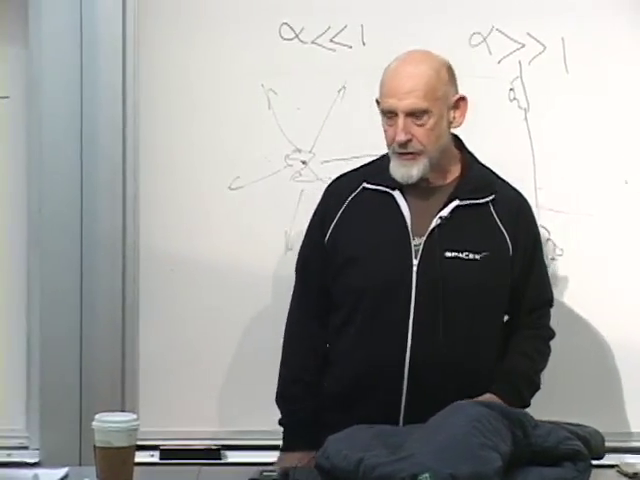
\includegraphics[width=0.72\textwidth]{lecture_01_figure_02.png}
\lectureframe{00:38:22.500}

\vspace{1em}

\begin{tikzpicture}[scale=0.95]
\draw (-5.3,-2.4) rectangle (-1.0,2.1);
\draw (0.3,-2.4) rectangle (4.6,2.1);

\node at (-3.15,2.55) {$\alpha \ll 1$};
\node at (2.45,2.55) {$\alpha \gg 1$};

\draw[line width=0.9pt] (-3.15,-0.15) circle (0.22);
\draw[->,line width=0.8pt] (-3.15,0.07) -- (-3.15,1.35);
\draw[->,line width=0.8pt] (-2.98,-0.01) -- (-1.95,1.00);
\draw[->,line width=0.8pt] (-3.32,-0.01) -- (-4.35,1.00);
\draw[->,line width=0.8pt] (-2.95,-0.23) -- (-1.80,-0.95);
\draw[->,line width=0.8pt] (-3.35,-0.23) -- (-4.50,-0.95);

\draw[line width=1.0pt] (2.15,-1.8) .. controls (1.95,-0.6) and (1.95,0.8) .. (2.15,1.55);
\draw[line width=1.0pt] (2.75,-1.8) .. controls (2.95,-0.6) and (2.95,0.8) .. (2.75,1.55);
\draw[line width=0.8pt] (2.15,-0.85) -- (2.75,-0.85);
\draw[line width=0.8pt] (2.45,1.55) -- (2.45,1.95);
\end{tikzpicture}
\caption{상호작용 에너지 논의에서 다룬 QED의 약결합--강결합 비교. 이 그림은 서스킨드가 설명하는 두 영역, 즉 희박한 약결합 구름과 증식하는 강결합 구름을 따로 보여준다.}
\end{figure}

약결합--강결합 비교가 앞서 도입되었는데도 이 그림이 여기에 놓인 이유는, 강의에서 서스킨드가 상호작용 에너지와 구조의 증식을 논하는 이 질문 중심의 대목에서 대조를 다시 그리기 때문이다.

\section{짝수 차원 브레인 이론과 창발하는 추가 차원}

여기까지 강의는 페르미온과 보손, 전자와 단극자, F-끈과 D-끈 사이의 교환을 강조해 왔다. 다음 단계는 더 놀랍다. 서스킨드는 홀수 차원 브레인 대신 짝수 차원 D-브레인을 갖는 다른 끈 이론으로 전환한다. 이 구분이 중요한 까닭은 이 이론에는 F-끈과 교환할 D-끈이 없기 때문이다. 여기에는 D0-브레인, D2-브레인, D4-브레인 등이 있다.

따라서 강결합 극한은 한 끈을 다른 끈으로 이름만 바꿔 부르는 것일 수 없다. 강의에 따르면 더 기묘한 일이 벌어진다. 추가 공간 차원이 뚜렷하게 드러난다. 서스킨드는 먼저 이를 가장 극적인 표현으로 말한다 --- ``새 차원이 모습을 드러낸다'' ---. 그리고 곧바로 더 신중한 진술로 바꿔 설명한다. 아주 작은 콤팩트 방향이 무시할 수 없을 때까지 커진다는 것이다.

장부를 맞추는 일도 논점의 일부이므로, 서스킨드는 여기서 잠시 멈춘다.
\begin{equation}
\begin{aligned}
10\text{-dimensional string theory} &= 9\text{ space}+1\text{ time},\\
11\text{-dimensional theory} &= 10\text{ space}+1\text{ time}.
\end{aligned}
\end{equation}
강의의 주장은 짝수 차원 브레인 이론의 강결합 극한이 사실상 11차원이라는 것이다.

\editorialnote{짝수 차원 브레인 이론은 IIA형 끈 이론이며, 그 강결합 완성은 M-이론이다. 표준 단위계에서 창발하는 원의 반지름과 11차원 플랑크 길이는 각각 \(R_{11}=g_s\ell_s\), \(\ell_{11}=g_s^{1/3}\ell_s\)로 주어진다. 이 명칭과 공식은 강의의 기하학적 설명 뒤에 있는 현대적 대응 관계를 명시적으로 보여준다.}

\subsection{땅콩버터 샌드위치}

콤팩트 방향을 그려 보기 위해 서스킨드는 ``땅콩버터 샌드위치'' 모형을 사용한다. 두 장의 무한히 얇은 빵 사이에 실제 공간이 있다고 생각하면 된다. 특별한 규칙은 한쪽으로 나가면 다른 쪽으로 돌아온다는 것이다. 강의에서는 형식적으로 쓰기보다 그림으로 설명하지만, 통상적인 표기로는 다음과 같이 쓸 수 있다.
\begin{equation}
y \sim y + 2\pi R.
\end{equation}
샌드위치 안에 사는 관측자가 보기에 \(R\)가 매우 작으면, 그들의 세계는 유효적으로 더 낮은 차원으로 기술된다. 그러면 강결합에서 핵심적인 변화는 다음과 같다.
\begin{equation}
g\uparrow
\qquad \Longrightarrow \qquad
R_{\mathrm{compact}}\uparrow.
\end{equation}
서스킨드가 새로운 공간 차원이 나타난다고 말하는 뜻은 이렇다. 공간이 무에서 생겨난다는 것이 아니라, 이전에는 아주 작았던 콤팩트 방향이 커져 유효 이론에서 보이게 된다는 것이다.

\begin{figure}[htbp]
\centering
\resizebox{\linewidth}{!}{%
\begin{tikzpicture}[scale=0.95]
\draw[line width=0.9pt] (-5,1.7) -- (5,1.7);
\draw[line width=0.9pt] (-5,-1.7) -- (5,-1.7);

\node[left] at (-5,1.7) {ceiling};
\node[left] at (-5,-1.7) {floor};

\draw[->,line width=0.8pt] (5.2,1.45) -- (5.2,-1.45);
\draw[->,line width=0.8pt] (5.5,-1.45) -- (5.5,1.45);
\node[right] at (5.55,0) {periodic};

\draw[line width=1.0pt] (-2.6,0.45) -- (2.2,0.45);
\draw[line width=1.0pt] (-2.6,-0.05) -- (2.2,-0.05);
\draw[line width=1.0pt] (-2.6,0.45) -- (-2.6,-0.05);
\draw[line width=1.0pt] (2.2,0.45) -- (2.2,-0.05);
\node at (-0.2,0.9) {floating D2-brane};

\draw[line width=1.0pt] (3.15,-1.7) -- (3.8,-1.7);
\draw[line width=1.0pt] (3.15,1.7) -- (3.8,1.7);
\draw[line width=1.0pt] (3.15,-1.7) -- (3.15,1.7);
\draw[line width=1.0pt] (3.8,-1.7) -- (3.8,1.7);
\node[right] at (3.95,0) {D2 ribbon};

\fill (-3.8,0) circle (0.07);
\node[below] at (-3.8,-0.05) {D0};
\end{tikzpicture}
}%
\caption{샌드위치 콤팩트화. 위와 아래의 경계는 주기적으로 동일시된다. D2-브레인 하나는 카펫처럼 그 사이에 떠 있고, 또 하나는 바닥에서 천장까지 뻗어 있으며 콤팩트 방향이 작을 때는 끈처럼 보인다.}
\end{figure}

\subsection{D0-브레인과 D2-브레인은 어떻게 되는가?}

이제 강의는 D0-브레인과 끈에 무슨 일이 일어나는지 묻는다. 답은 서로 다르다. \(g\)가 커질수록 D0-브레인은 점점 가벼워진다. 고차원 해석에서는 새롭게 드러난 방향으로 운동량을 지닌 입자들의 탑에 합류한다. 따라서 약결합 그림에서 무겁고 복잡한 대상이 강결합 그림에서는 평범하고 가벼운 여기로 바뀐다.

질량 관계는 이러한 동일시를 보여준다.
\begin{equation}
M_{D0}(n)=\frac{n}{g_s\ell_s}
=\frac{n}{R_{11}}
=M_{\mathrm{KK}}(n).
\end{equation}
\editorialnote{서스킨드는 D0-브레인을 11차원 이론의 ``중력자''라고 부른다. 더 정확히는 이들의 결합 상태가 11차원 초중력 다중항의 칼루차--클라인 운동량 모드이며, 그 질량 없는 부문에 중력자가 포함된다. 이렇게 구분하면 강의에서 제시하는 물리적 동일성을 유지하면서 한 입자에 대한 문자 그대로의 과장된 진술은 피할 수 있다.}

D2-브레인은 끈의 운명을 설명한다. 강의에서 강조하는 배치는 두 가지다.
\begin{enumerate}
\item 땅콩버터 속 카펫처럼 바닥과 천장 사이에 떠 있는 D2-브레인,
\item 보이는 방향을 따라 뻗어 리본처럼 바닥에서 천장까지 이어진 D2-브레인.
\end{enumerate}샌드위치가 얇을 때 이 리본은 유효적으로 1차원처럼 보인다. 저에너지 관측자가 끈이라고 부르는 대상이 바로 이것이다. 콤팩트 방향이 열리면 같은 대상은 분명한 막의 형태를 띤다. 이제 수직 방향으로 더 많은 물질을 포함하므로 무거워지고 끈의 모습에서 멀어진다.

\paragraph{전이의 논리.}
\begin{enumerate}
\item 먼저 아주 작은 콤팩트 방향을 생각하자. 바닥에서 천장까지 이어진 리본은 사실상 끈처럼 거동한다.
\item \(g\)를 키우면 콤팩트 방향이 팽창한다.
\item 0-브레인은 가벼워져 고차원 이론의 칼루자--클라인 운동량 상태로 재해석된다.
\item 끈처럼 보이던 D2 리본은 눈에 띄게 펼쳐진 막이 되어 무거워진다.
\end{enumerate}
이 대목은 이중성에서 창발적 기하로 넘어가는 강의의 전환점이다. 강한 결합은 단순히 한 물체를 다른 물체로 바꾸는 데 그치지 않는다. 어느 기하가 더 효율적인지를 바꾼다.

Susskind는 이 설명이 얼마나 낯설게 들리는지 잠시 짚고 넘어간다. 제안된 여러 식별 관계가 성립하려면 까다로운 수학적 일관성 관계가 필요했으며, 그중 일부는 처음에는 물리학자들의 추측으로 제시되었다가 나중에 수학자들에 의해 증명되었다. 그의 주장은 모든 현실적인 끈 진공을 이해했다는 것이 아니라, 이중성의 연결망 자체가 이례적으로 엄격한 검증을 견뎌 왔다는 것이다.

이 이상화된 설정에서 결합상수가 위치에 따라 달라지면, 그에 따라 효율적인 기하도 달라질 수 있다. 한 영역은 가벼운 끈과 무거운 D0-브레인이 있는 거의 10차원 공간처럼 보일 수 있고, 다른 영역은 무거운 감긴 막과 가벼운 칼루자--클라인 모드가 있는 11차원 기술로 열릴 수 있다. 국소적으로 기술 방식이 달라지는 것도 같은 이중성 연결망의 일부다.

녹취록에는 이 관계의 이름이 ``부등식''으로 잠시 잘못 기록되어 있다. 문맥상 의도된 단어는 \emph{이중성}이다. 이는 매개변수 공간의 서로 반대쪽 끝을 잇는 관계를 뜻한다. 이 정정이 중요한 이유는 강의의 결론이 바로 근본 구성 요소의 유일한 목록은 알려져 있지 않다는 것이기 때문이다. 끈, 브레인, 입자, 고차원 기하는 서로 변환될 수 있다. 이 연결망에서 어느 구성원도 절대적으로 근본적이지 않거나, 아니면 더 깊은 구조가 아직 알려지지 않은 것이다.

\section{D3-브레인, 감긴 막, 그리고 이중성의 기하학적 그림}

휴식 후 Susskind는 이 주제를 서로 연결된 이론과 아이디어의 ``거대한 연결망''이라고 명시적으로 설명한다. 이어지는 예들은 각각 따로 떨어진 새로운 현상이 아니라, 앞서 나온 설명들을 서로 이어 주는 다리다.

\subsection{D3-브레인 월드볼륨}

첫 번째 다리에는 D3-브레인이 등장한다. D3-브레인은 공간 차원이 3개이므로, 그 위에 갇힌 관찰자는 그것을 평범한 공간으로 쉽게 오인할 수 있다. 브레인은 휘고 요동할 수 있으며, 브레인에 끝점을 둔 끈은 결합하거나 갈라지고 산란할 수 있다. 브레인 방향만 보는 관찰자에게 각 끝점은 입자로 보이고, 끝점들 사이의 상호작용은 보통의 양자장론처럼 보인다.

\begin{figure}[htbp]
\centering
\resizebox{\linewidth}{!}{%
\begin{tikzpicture}[scale=1.0]
\draw[fill=gray!15] (-4,-0.35) rectangle (4,0.35);
\node at (0,-0.75) {D3-brane};

\draw[line width=0.9pt] (-1.5,2.1) -- (-1.5,0.35);
\fill (-1.5,0.35) circle (0.07);
\node[left] at (-1.72,1.25) {F-string};
\node[below left] at (-1.5,0.32) {electric charge};

\draw[line width=1.5pt] (1.7,2.1) -- (1.7,0.35);
\fill (1.7,0.35) circle (0.09);
\node[right] at (1.95,1.25) {D-string};
\node[below right] at (1.7,0.32) {magnetic monopole};
\end{tikzpicture}
}%
\caption{D3-브레인 월드볼륨 해석. F-끈의 끝점은 전하로 보이고, D-끈의 끝점은 자기 홀극으로 보인다.}
\end{figure}

이는 강의에서 가장 만족스러운 식별 관계 중 하나다. D3-브레인에 끝점을 둔 F-끈은 월드볼륨 관찰자에게 전하로 보인다. 같은 브레인에 끝점을 둔 D-끈은 자기 홀극으로 보인다. 다시 말해 F-끈과 D-끈 사이의 이중성은 D3-브레인 월드볼륨에서 보통의 장론에 나타나는 전기--자기 이중성이 된다. 앞서 비유였던 것이 이제 명시적인 대응표가 된다.

\editorialnote{D3-브레인 다발의 저에너지 월드볼륨 기술은 4차원 \(\mathcal N=4\) 초대칭 양--밀스 이론이다. 이 이론의 전기--자기 이중성은 IIB형 끈 이론의 S-이중성이 장론에서 구현된 것이다. 브레인 하나의 경우에는 강의에서 그림으로 사용한 아벨 극한에 해당한다.}

\subsection{두 콤팩트 방향과 비대칭 감기}

이어서 Susskind는 고차원 기하로 돌아가 작은 방향을 하나가 아니라 둘 콤팩트화한다. 11차원을 칠판에 그릴 수는 없으므로, 그림에 쓰이지 않는 큰 방향 일곱 개를 눈에 보이는 수평 방향 하나로 압축하고 두 콤팩트 방향은 따로 그린다. 그는 콤팩트화가 비대칭이 되도록 그려야 한다고 강조한다. 유효 끈들의 장력이 서로 다르려면 한 콤팩트 방향이 다른 방향보다 짧아야 하기 때문이다.

\begin{figure}[htbp]
\centering
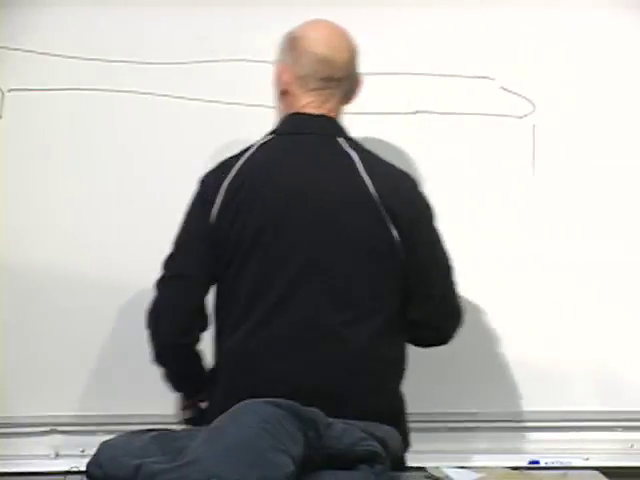
\includegraphics[width=0.78\textwidth]{lecture_01_figure_03.png}
\lectureframe{01:10:25.000}
\caption{두 감긴 막의 완성된 칠판 그림. 짧고 긴 콤팩트 주기가 오른쪽에 그려진 F-끈 및 D-끈 형태의 리본을 만든다.}
\end{figure}

막은 두 콤팩트 방향 중 어느 쪽으로든 감길 수 있으며, 비콤팩트 방향에서 보면 끈처럼 보인다. 두 원의 반지름이 \(R_1\)와 \(R_2\)라면 유효 장력은 다음과 같다.
\begin{equation}
\begin{aligned}
T_{(1)}&=2\pi R_1 T_{\mathrm{M2}},\\
T_{(2)}&=2\pi R_2 T_{\mathrm{M2}},\\
\frac{T_{(1)}}{T_{(2)}}&=\frac{R_1}{R_2}.
\end{aligned}
\end{equation}
따라서 원의 크기가 다르면 끈의 장력도 다르다. 더 짧은 방향으로 감긴 끈을 가벼운 F-끈으로, 더 긴 방향으로 감긴 끈을 무거운 D-끈으로 보면 개략적으로 다음과 같이 쓸 수 있다.
\begin{equation}
g_s\sim \frac{R_{\mathrm{short}}}{R_{\mathrm{long}}},
\qquad
\frac{T_{\mathrm{D1}}}{T_{\mathrm{F1}}}\sim \frac{1}{g_s}.
\end{equation}

\begin{classroomqa}
\audiencequestion{이 그림에서 결합상수를 두 콤팩트 차원의 비로 이해할 수 있습니까? \lecturetimestamp{01:10:13}}
\lecturerresponse{그렇다. 약--강 결합 매개변수는 종횡비로 기하학적으로 표현된다. 한 방향을 짧게 만들면 결합상수가 작아지고, 두 방향을 서로 맞바꾸면 가벼운 끈과 무거운 끈도 서로 바뀐다.}
\end{classroomqa}

\editorialnote{강의에서는 이 비를 잠시 \(\alpha\)라고 부르는데, 이는 앞서 양자전기역학의 미세구조상수를 나타낼 때 쓴 기호를 다시 사용한 것이다. 두 의미를 구별하기 위해 여기서는 \(g_s\)라고 쓴다. 완전한 M-이론 구성에서 IIB형 끈 이론의 결합상수는 콤팩트한 2차원 토러스의 복소구조에 담긴다. 분자의 정확한 형태는 토러스의 주기를 어떻게 이름 붙이느냐에 따라 달라진다.}

감긴 막의 그림은 칠판 그림의 원근 왜곡 없이 다음과 같이 요약할 수 있다.

\begin{figure}[htbp]
\centering
\begin{tikzpicture}[scale=1.0]
\draw[line width=0.9pt] (0,0) rectangle (5.2,2.2);
\node[below] at (2.6,-0.2) {\(R_1\)};
\node[right] at (5.4,1.1) {\(R_2\)};

\draw[->,line width=0.7pt] (5.45,1.9) -- (5.45,0.3);
\draw[->,line width=0.7pt] (5.7,0.3) -- (5.7,1.9);
\draw[->,line width=0.7pt] (0.4,-0.35) -- (4.8,-0.35);
\draw[->,line width=0.7pt] (4.8,-0.6) -- (0.4,-0.6);

\draw[line width=1.0pt] (1.1,0) -- (1.6,0) -- (1.6,2.2) -- (1.1,2.2) -- cycle;
\node at (1.35,2.55) {light};

\draw[line width=1.0pt] (0,1.45) -- (5.2,1.45);
\draw[line width=1.0pt] (0,1.00) -- (5.2,1.00);
\node at (4.55,1.95) {heavy};

\node at (1.35,-0.95) {F-string};
\node at (4.55,0.55) {D-string};
\end{tikzpicture}
\caption{감긴 막의 두 배치는 모두 비콤팩트 방향에서 끈처럼 보이지만, 콤팩트 방향의 크기가 다르면 한 유효 끈이 다른 끈보다 가벼워진다.}
\end{figure}

이는 앞서 살펴본 이중성 이야기의 기하학적 표현이다. 한 방향을 압축하는 동시에 다른 방향을 늘리면 감긴 물체 하나는 무거워지고 다른 하나는 가벼워져 F-끈과 D-끈의 역할이 서로 바뀔 수 있다.

\begin{classroomqa}
\audiencequestion{콤팩트 방향이 주기적이라면 감긴 물체는 폭이 무한합니까? \lecturetimestamp{01:10:41}}
\lecturerresponse{아니다. 콤팩트 원은 끝에 도달하지 않고 계속 돌 수 있지만 둘레는 유한하다. 잘라 펼친 그림의 위쪽과 아래쪽은 같은 점을 나타낸다. 구간의 양 끝점이 원의 한 점을 나타낼 수 있는 것과 같다.}
\end{classroomqa}

\begin{figure}[htbp]
\centering
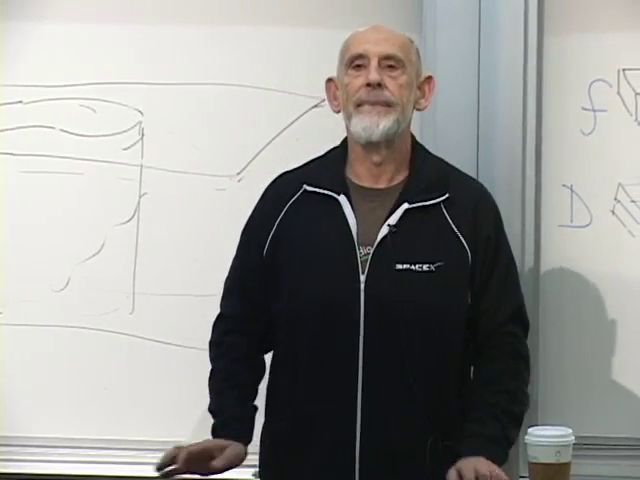
\includegraphics[width=0.78\textwidth]{lecture_01_figure_04.png}
\lectureframe{01:12:25.000}

\vspace{1em}

\begin{tikzpicture}[scale=0.95]
\draw[line width=0.9pt,->] (-3.7,0) arc[start angle=180,end angle=535,radius=0.95];
\node at (-2.75,0) {compact circle};
\draw[line width=0.9pt] (0.0,0) -- (4.8,0);
\fill (0.0,0) circle (0.06);
\fill (4.8,0) circle (0.06);
\draw[<->] (0.0,-0.45) -- (4.8,-0.45);
\node at (2.4,-0.75) {cut-open interval of length \(2\pi R\)};
\node[above] at (0.0,0.1) {same point};
\node[above] at (4.8,0.1) {same point};
\end{tikzpicture}
\caption{콤팩트 원과 그것을 칠판에서 잘라 펼쳐 나타낸 그림. 한쪽 끝점을 지나면 다른 쪽에서 이어진다. 원을 따라 움직이는 동시에 비콤팩트 방향으로도 이동하면 나선이 그려진다.}
\end{figure}

\begin{classroomqa}
\audiencequestion{콤팩트 경로는 왜 나선이 아니라 원입니까? \lecturetimestamp{01:12:23}}
\lecturerresponse{비콤팩트 방향의 각 고정된 점에서 콤팩트 방향은 원이다. 나선은 원을 따라 감기는 동시에 비콤팩트 방향으로 나아갈 때만 나타난다. 칠판의 구간은 단지 원을 잘라 펼친 것으로, 양 끝점은 서로 동일시된다.}
\end{classroomqa}

\begin{classroomqa}
\audiencequestion{이 기하 자체가 D-브레인을 가까이서 관측했을 때 F-끈들의 집합처럼 보이는 이유를 설명합니까? \lecturetimestamp{01:12:49}}
\lecturerresponse{둘 사이의 연결은 있지만, 이 기초적인 그림에서는 분명하게 드러나지 않는다. 이를 보려면 더 많은 기하학적 도구가 필요하다. 이 그림은 이중성을 정리하기 위한 것이지, 모든 미시적 구성 요소의 기술을 유도하기 위한 것은 아니다.}
\end{classroomqa}

\begin{classroomqa}
\audiencequestion{공간을 따라 이동하거나 시간이 흐르면서 긴 콤팩트 방향과 짧은 콤팩트 방향이 서로 바뀔 수 있습니까? \lecturetimestamp{01:13:35}}
\lecturerresponse{이상화된 모형에서는 둘 다 가능하다. 한 주기를 압축하고 다른 주기를 팽창시키면 어느 감긴 끈이 가벼운지가 바뀐다. 이것이 ``근본 끈''이란 명칭일 뿐인 또 하나의 이유다. 선호되는 기술 방식은 영역마다, 또는 시간에 따라 달라질 수 있다.}
\end{classroomqa}

\section{이상화, 특별히 대칭적인 점, 그리고 랜드스케이프}

강의의 마지막 부분에서 Susskind는 우아한 이중성의 예들에서 한 걸음 물러나, 그것들이 현실 세계에 대해 무엇을 말해 주며 무엇을 말해 주지 않는지 묻는다.

먼저 Susskind는 정밀하게 다룰 수 있는 이중성들이 보손과 페르미온의 질량이 정확히 일치하는 고도로 이상화된 초대칭 이론의 특징이라고 경고한다. 그는 뉴턴 역학의 원운동에 비유한다. 원운동은 대칭적이고 수학적으로 다루기 쉬우므로 먼저 연구하는 것이지, 실제 행성 운동이 완전한 원운동만으로 설명되기 때문은 아니다. 마찬가지로 초대칭 끈 이론은 자연보다 대칭성이 높아 분석하기 쉽다.

그렇다고 이상화가 유익하지 않은 것은 아니다. 완벽한 원운동은 현실적인 행성계는 아니지만, 대칭성이 낮은 궤도에서도 남아 있는 특징을 보여 준다. 마찬가지로 초대칭 사례들은 양자역학, 중력, 미시적 구조가 서로 모순 없이 결합할 수 있는 방식을 보여 준다. Susskind는 일부러 단호하게 말한다. 다루기 쉬운 끈 이론들은 문자 그대로 우리 세계의 이론이 아니다. 그 가치는 대칭성이 낮고 다루기 어려운 상황에서도 다시 나타날 가능성이 있는 현상을 드러낸다는 데 있다.

\subsection{여러 결과를 낳는 구성 도구}

D-브레인은 사용할 수 있는 구성 도구의 일부일 뿐이다. 강의에서는 플럭스, 오비폴드, 오리엔티폴드도 언급한다. 먼저 콤팩트 기하를 고른 다음, 어떤 브레인과 플럭스가 그 주기를 차지할지 선택한다. 간단한 샌드위치 모형조차 떠 있는 D2-브레인을 하나, 둘, 셋 넣느냐에 따라 저차원 물리가 달라진다. 이런 요소를 더하거나 빼면 유효 입자와 상호작용, 매개변수가 바뀐다.

강의에서 제시한 개략적인 수를 생각해 보자. 6차원 콤팩트 공간에 대략 \(500\)개의 주기가 있고, 각 주기에서 감긴 브레인이나 플럭스 또는 관련 구조를 고르는 방법이 대략 \(10\)가지라면, 구성의 수는 다음과 같이 증가한다.
\begin{equation}
N_{\mathrm{vacua}} \sim 10^{500}.
\end{equation}
강의의 계산 논리는 간단하다.
\begin{equation}
10 \times 10 \times \cdots \times 10 = 10^{500}
\end{equation}
여기서 인자는 \(500\)개다. DNA 비유를 들면 같은 점을 더 친숙한 방식으로 표현할 수 있다.
\begin{equation}
N_{\mathrm{DNA}}(500)=4^{500}.
\end{equation}
DNA를 비교하는 중에 청중 한 명이 한 가닥을 따라 가능한 선택지가 A, C, G, T 네 가지인지 확인한다. 이 정정은 주장을 바꾸지 않고 오히려 뒷받침한다. 몇 가지 국소적 선택을 여러 번 반복하면 전역적으로는 방대한 수의 배치가 생긴다. 정확한 지수가 핵심은 아니며, Susskind는 \(10^{500}\)이라는 수를 오래된 과소 추정치라고 부른다. 핵심은 조합론적 증식이다.

이로써 도입부에서 제기한 환원주의적 기대가 뒤집힌다. 복잡한 입자물리학이 반드시 복잡한 미시적 법칙에서 나오는 것은 아니다. 복잡한 유기체가 네 가지 염기로 이루어진 서열에 부호화될 수 있듯, 우리의 진공이 단순한 요소들을 복잡하게 배열한 결과일 수 있다.

\begin{classroomqa}
\audiencequestion{이중성으로 연결된 동등한 기술들을 하나로 묶고 나면, 완전한 정보가 가능한 진공들 가운데 우리 세계를 기술하는 하나 또는 몇 개만을 가려낼 수 있을까요? \lecturetimestamp{01:26:11}}
\lecturerresponse{아마도 제한된 집합을 골라낼 것이다. 하지만 서로 다른 여러 진공이 관측 가능한 에너지 범위에서는 매우 비슷해 보일 수 있다. 인용된 랜드스케이프의 수는 이중적인 기술을 하나로 묶은 뒤에도 여전히 크다는 뜻이다. 중요하지 않은 고에너지 세부 사항은 ``쓸모없는 DNA''}처럼 작용할 수도 있다.\end{classroomqa}

\subsection{대칭적인 점과 일반적인 복잡성}

랜드스케이프 안에는 특별히 대칭적인 점들이 있다. 기하학적 그림에서 두 방향의 종횡비가 같은 배치,
\begin{equation}
R_1=R_2,
\end{equation}
에서는 두 감긴 기술이 똑같이 단순해진다. 전기--자기 비유에서는 이를 개략적으로 다음과 같이 나타낸다.
\begin{equation}
m_{\mathrm{monopole}}=m_e.
\end{equation}

\begin{figure}[htbp]
\centering
\begin{tikzpicture}[scale=0.95]
\draw[line width=0.9pt] (-4.5,-1.0) rectangle (-2.5,1.0);
\draw[<->] (-4.5,-1.35) -- (-2.5,-1.35);
\draw[<->] (-2.15,-1.0) -- (-2.15,1.0);
\node at (-3.5,1.45) {symmetric point};
\node at (-3.5,-1.75) {$R_1=R_2$};

\draw[line width=0.9pt] (0.0,-0.55) rectangle (4.8,0.55);
\draw[<->] (0.0,-0.9) -- (4.8,-0.9);
\draw[<->] (5.15,-0.55) -- (5.15,0.55);
\node at (2.4,1.45) {lopsided point};
\node at (2.4,-1.3) {$R_1\ne R_2$};
\end{tikzpicture}
\caption{종횡비가 같은 콤팩트화에서는 두 감긴 끈이 대칭적으로 다뤄진다. 한쪽으로 치우친 콤팩트화에서는 한 기술이 다른 기술보다 훨씬 가벼워진다.}
\end{figure}

\begin{classroomqa}
\audiencequestion{랜드스케이프에서 F-끈과 D-끈의 기술이 일치해 구성이 훨씬 단순해지는 진공도 있습니까? \lecturetimestamp{01:27:21}}
\lecturerresponse{그렇다. 특별히 대칭적인 점들이 있다. 우리 세계는 그중 하나에 있는 것으로 보이지 않는다. 익숙한 전기적 입자와 자기 홀극의 질량은 같지 않다. 자연이 한쪽으로 치우친 점에 놓인 이유는 알려져 있지 않다.}
\end{classroomqa}

\editorialnote{전자--홀극 질량이 같다는 것은 적절히 보호된 자기이중 모형에서 나타나는 개략적 특성이지, 보통의 비초대칭 양자전기역학이 예측하는 바가 아니다. 이는 관측된 전자에 관한 주장이 아니라 강의에서 말하는 대칭점의 개념을 표현한다.}

이어서 Susskind는 통신 이론의 비유를 든다. 무작위 부호는 놀라울 만큼 성능이 좋을 수 있지만, 기술하고 해독하기 쉬운 부호는 수학적 구조를 더 갖추고 있어 역사적으로 성능이 더 낮았다. 이후 부호 이론에서는 구조를 갖추면서도 매우 효과적인 구성이 발견되었지만, 비유의 요지는 여전히 유효하다. 간결한 이름이나 설명으로 나타낼 수 있는 것은 가능성 전체 공간에서 복잡도가 낮은 매우 특별한 부분에 속한다. 마찬가지로 계산하기 가장 쉬운 끈 진공은 전형적이지 않을 수 있다.

따라서 적절한 질문도 달라질 수 있다. 미시적 세부 사항까지 모두 포함한 정확한 콤팩트화를 요구하는 대신, 폭넓은 앙상블에서 어떤 특징이 공통적이거나 일반적인지 물을 수 있다. Susskind는 이를 확정된 결론이 아니라 연구 과제로 제시하며, 계산 대신 이념적 주장을 내세우는 것을 거부한다.

\subsection{우주론적 질문}

\begin{classroomqa}
\audiencequestion{둘레가 엄청나게 큰 콤팩트 방향은 무한한 방향과 관측상 구별됩니까? 우리에게 큰 공간 차원이 3개 있다는 것은 알지만, 그 차원들이 무한하다는 것도 알고 있습니까? \lecturetimestamp{01:30:03}}
\lecturerresponse{그 차원들이 무한하다는 사실은 알지 못한다. 닫힌 3차원 구면은 콤팩트한 채로 팽창할 수 있다. 거의 평평하다는 측정 결과는 곡률 반지름의 하한만 제공한다. 거의 평평한 들판을 측량해 지구의 크기에 상한을 둘 수는 있어도, 지구 표면이 무한하다는 것을 증명할 수는 없는 것과 같다. 유한한 규모를 결정하려면 곡률을 검출하거나 전역적 동일시를 확인해야 한다.}
\end{classroomqa}

\begin{classroomqa}
\audiencequestion{이상화된 모형에서 결합 상수가 공간에 따라 달라질 수 있다면, 현실 세계에서는 그런 변화가 어떻게 일어날 수 있을까요? \lecturetimestamp{01:32:43}}
\lecturerresponse{대칭적인 예에서 사용한 것처럼 제한 없이 연속적으로 변하는 방식으로는 일어나지 않습니다. 뒤에서 논의할 현실적인 가능성은 서로 다른 유효 법칙을 따르는 영역들 사이의 이산적 전이를 통해 변하는 것입니다. 그런 도약이 일어나는지는 우주론의 문제입니다.}
\end{classroomqa}

\editorialnote{이 답변은 모든 스칼라장이 매끄럽게 변할 수 없다는 일반 정리가 아니라, 플럭스 진공과 영역 전이에 대한 강의의 예고로 읽어야 한다. 관측은 무차원 결합상수의 변화를 강하게 제한하며, 주어진 모형에서 연속적인 모듈라이가 남아 있는지는 안정화 메커니즘에 달려 있다.}

녹음에는 마지막 청중 질문이 남아 있지 않다. 보존된 답변에 따르면 제안된 현상은 일부 종류의 블랙홀에서는 일어날 수 있지만, 자유 낙하 관찰자에게 국소적으로 평범한 장소인 보통의 슈바르츠실트 블랙홀 지평선에서는 일어나지 않는다. 질문 내용을 신뢰성 있게 복원할 수 없으므로, 이 대화에 더 구체적인 주장을 덧붙이지 않는다.

\section{벽돌에서 기술의 연결망으로}

물리학의 더 깊은 층위는 반드시 더 단순해야 한다는 기대는 취약한 것으로 드러났다. \(1+1\)차원 보손화에서는 같은 이론을 페르미온 중심으로 구성할 수도 있고 보손 중심으로 구성할 수도 있으며, 이때 페르미온은 킨크로 다시 나타난다. 양자전기역학에서는 약결합과 강결합에 따라 전자와 자기 홀극의 기술상 역할이 서로 바뀐다. 끈 이론에서는 F-끈과 D-끈이 같은 양상을 되풀이한다. 브레인이 짝수 개인 이론에서는 강결합이 한 걸음 더 나아간다. 콤팩트 방향이 팽창하고, D0-브레인은 칼루자--클라인 운동량 상태가 되며, 유효 끈은 고차원 기하에서 감긴 막으로 재해석된다. 따라서 현대 양자장론과 끈 이론은 ``어느 것이 벽돌이고 어느 것이 집인가?''라는 질문에 단번에 고정된 유일한 답을 주지 않는다. 각 기술이 자기 영역에서 효율적인 기술들의 연결망과, 일반적인 결과가 단순함보다 복잡성인 방대한 가능성의 랜드스케이프를 제시한다.

\chapter{기하학, 정보, 블랙홀 면적 법칙}

\lectureoverview{예고된 목적지는 우주론이지만, 그곳으로 가는 가장 짧은 길은 특수 상대론을 다시 살펴보는 데서 시작한다. 계량은 시공간의 기하학을 알려 주고, 고유 시간이 0이라는 조건은 빛이 어떻게 움직이는지 알려 준다. 이 규칙 하나를 슈바르츠실트 기하학에 적용하고, 지평선과 특이점을 구별한 다음, 블랙홀이 복사를 내며 사라질 때 정보가 어떻게 되는지 묻겠다. 답은 보통의 엔트로피에서 시작해 베켄슈타인의 비트 하나 논증으로 끝난다. 블랙홀은 정보를 부피가 아니라 지평선 면적 단위로 저장한다.}

서스킨드는 끈 이론의 성과와 실패를 약속한 대로 따져 보는 일을 잠시 미룬다. 늦은 시간이고, 평가보다 핵심 내용을 다루는 편이 더 유익하다고 말한다. 오늘 밤의 핵심은 블랙홀 정보 문제를 정식화하는 데 필요한 최소한의 기하학과 열역학이다.

\section{빛에 관한 하나의 규칙}

특수 상대론은 공간과 시간을 하나의 기하학적 대상으로 다룬다. 서로 \(dt,dx,dy,dz\)만큼 떨어진 이웃한 사건에 대해 서스킨드는 시간 항의 부호가 양수인 관례를 택해 다음과 같이 쓴다.
\begin{equation}
d\tau^2=dt^2-\frac{1}{c^2}\left(dx^2+dy^2+dz^2\right).
\end{equation}
시간 성분과 공간 성분의 부호가 서로 다르다는 점에서 민코프스키 기하학은 4차원 유클리드 기하학과 구별된다. 인자 \(1/c^2\)는 단위만 맞춰 준다. 시간과 거리를 일관된 단위로 측정하면 \(c=1\)로 둘 수 있다.

시간꼴 간격에서는 \(d\tau^2>0\)이고, \(d\tau\)은 그 궤적을 따라가는 시계가 기록하는 고유 시간이다. 공간꼴 간격에서는 반대로 \(d\tau^2<0\)이다. 오늘 필요한 경우는 그 두 경우의 정확한 경계에 놓인다. 빛은 \emph{널} 궤적을 따른다.
\begin{equation}
d\tau^2=0.
\end{equation}
먼저 \(x\)축 방향의 운동으로 한정하면 다음을 얻는다.
\begin{align}
0&=dt^2-\frac{dx^2}{c^2},\\
c\,dt&=\pm dx,\\
\frac{dx}{dt}&=\pm c.
\end{align}
부호는 오른쪽으로 진행하는 광선과 왼쪽으로 진행하는 광선을 나타낸다. 센티미터를 미터나 킬로미터로 바꾸면 \(c\)에 부여되는 수치가 달라진다. 불변인 진술은 수치가 아니라 널 조건이다.

일반 상대론에서는 이 규칙이 아니라 계량이 복잡해진다. 좌표가 \(x^\mu\)이고 \(\mu=0,1,2,3\)일 때,
\begin{equation}
ds^2=g_{\mu\nu}(x)\,dx^\mu dx^\nu,
\end{equation}
여기서 반복된 지표에 대해서는 합산하며, 계수는 위치에 따라 달라질 수 있다. 빛이 국소적으로 진행할 수 있는 방향을 찾으려면 이 이차 형식을 0으로 놓으면 된다.

\section{구면 좌표와 슈바르츠실트 계량}

회전하지 않는 블랙홀은 구대칭이므로, 데카르트 좌표로는 유용한 구조가 잘 드러나지 않는다. \(r\)를 반지름 방향 거리로, \(\theta,\phi\)를 단위 구면 위의 방향을 나타내는 좌표로 두자. 구면의 선요소는 다음과 같다.
\begin{equation}
d\Omega^2=d\theta^2+\sin^2\theta\,d\phi^2.
\end{equation}
반지름이 \(r\)인 구면에서는 각방향 변위가 따라서 \(r^2d\Omega^2\)만큼 기여한다. 구면 좌표로 쓴 평탄한 시공간은 다음과 같다.
\begin{equation}
d\tau^2=dt^2-\left(dr^2+r^2d\Omega^2\right),
\qquad (c=1).
\end{equation}

서스킨드는 아인슈타인 방정식에서 블랙홀 해를 유도하지 않는다. 식을 적어 놓고 살펴보자고 한다. 칠판에는 비교하려는 대상이 명확히 드러나 있다.

\begin{figure}[htbp]
\centering
\includegraphics[width=0.86\textwidth]{lecture_02_figure_02.png}
\caption{위쪽에는 평탄한 구면 시공간, 아래쪽에는 슈바르츠실트 변형이 그려져 있다. 반복되는 인자 \(1-2GM/(c^2r)=1-R_s/r\)와 반지름 방향 스케치가 함께 보인다.}
\lectureframe{00:19:12.520}
\end{figure}

질량이 \(M\)인 블랙홀에 대해 슈바르츠실트 반지름을 다음과 같이 정의하자.
\begin{equation}
R_s=\frac{2GM}{c^2}.
\end{equation}
외부 영역의 선요소는 다음과 같다.
\begin{equation}
d\tau^2=\left(1-\frac{R_s}{r}\right)dt^2
-\frac{dr^2/c^2}{1-R_s/r}
-\frac{r^2}{c^2}d\Omega^2.
\label{eq:schwarzschild-explicit-c}
\end{equation}
동등하게, \(c=1\)로 두면 다음과 같이 쓸 수 있다.
\begin{equation}
ds^2=\left(1-\frac{2GM}{r}\right)dt^2
-\frac{dr^2}{1-2GM/r}-r^2d\Omega^2.
\label{eq:schwarzschild}
\end{equation}
멀리 떨어진 곳에서는 \(R_s/r\ll1\)이므로 평탄한 구면 계량으로 돌아간다. 이 점근적 검산은 공식을 외우는 것보다 중요하다. 그래도 서스킨드는 칵테일 파티에서 이야기할 거리로 공식을 외워 두라고 권한다.

\editorialnote{칠판에서는 \(d\tau^2\)와 \(ds^2\)를 번갈아 쓰며, 인자 \(c\)를 일관되게 모두 표시하지는 않는다. 식~\eqref{eq:schwarzschild-explicit-c}은 시간 좌표에 관한 강의의 관례를 따르며, 이때 \(t\)의 단위는 시간이다. \(x^0=ct\)를 쓰는 표준형도 대수적으로 동등하다.}

\subsection{지평선은 특이점이 아니다}

좌표상 두 반지름에서 이상한 점이 보인다. 자연 단위계에서 \(r=R_s=2GM\)일 때 \(dt^2\)의 계수는 사라지고 \(dr^2\)의 계수는 발산한다. \(r=0\)에서는 곡률 자체가 특이해진다. 이는 같은 현상의 두 가지 표현이 아니다:
\begin{equation}
\begin{aligned}
r=R_s &:\quad \text{horizon},\\
r=0 &:\quad \text{curvature singularity}.
\end{aligned}
\end{equation}

조석력으로 두 경우의 물리적 차이를 알 수 있다. 중력장은 크기가 있는 물체의 위치에 따라 달라진다. 발이 머리보다 더 큰 힘을 받아 몸이 늘어나고, 가로 방향은 압축될 수 있다. 지평선에서 조석력은 유한하며, 충분히 무거운 블랙홀의 지평선에서는 아주 작을 수도 있다. 그곳에서 국소적으로 재앙적인 일이 반드시 일어나는 것은 아니다. 반면 \(r=0\)에서는 조석력이 발산한다. \(r=R_s\)에서 나타나는 문제의 계수는 슈바르츠실트 좌표의 결함을 나타내지만, \(r=0\)의 특이점은 물리적인 특이점이다.

\editorialnote{곡률이 \(r=R_s\)에서 유한하다는 점은 크레치만 스칼라 \(R_{\mu\nu\rho\sigma}R^{\mu\nu\rho\sigma}=48G^2M^2/(c^4r^6)\)로 확인할 수 있다. 이 값은 지평선에서 유한하고 \(r\to0\)일 때만 발산한다. 이 불변량은 강의 중 칠판에 쓰이지 않았지만, 조석력에 관한 구별을 정확히 해 준다.}

\section{지평선 부근의 방사형 광선}

이제 하나의 규칙으로 돌아가자. 방사형 광선은 각좌표를 고정한 채 진행하므로 \(d\Omega=0\)이고, 빛의 광선은 \(ds^2=0\)이다. \(c=1\) 단위계에서 식~\eqref{eq:schwarzschild}은 다음을 준다.
\begin{equation}
0=\left(1-\frac{2GM}{r}\right)dt^2
-\frac{dr^2}{1-2GM/r}.
\end{equation}
양변에 \(1-2GM/r\)를 곱하고 제곱근을 취하면 두 갈래가 나온다.
\begin{align}
dr&=\pm\left(1-\frac{2GM}{r}\right)dt,\\
\frac{dr}{dt}&=\pm\left(1-\frac{2GM}{r}\right).
\label{eq:radial-null}
\end{align}
양의 부호는 바깥쪽으로 나가는 광선, 음의 부호는 안쪽으로 들어가는 광선을 나타낸다. 멀리 떨어진 곳에서는 이들의 좌표 속도가 \(\pm1\)에 가까워진다. 지평선에서는 두 경우 모두 \(\lvert dr/dt\rvert\to0\)를 만족한다. 슈바르츠실트 좌표 시간으로 보면 바깥쪽 광선은 그곳에서 정지한 것처럼 보이고, 안쪽 광선은 도달하는 데 무한한 좌표 시간이 걸린다.

\begin{figure}[htbp]
\centering
\includegraphics[width=0.82\textwidth]{lecture_02_figure_03.png}
\caption{완성된 \(t\)-\(r\) 칠판 스케치. 점선 지평선에 가까워질수록 방사형 널 광선은 수직에 가까워진다.}
\lectureframe{00:30:25.000}
\end{figure}

\begin{figure}[htbp]
\centering
\begin{tikzpicture}[x=1.0cm,y=0.9cm]
\draw[->] (0,0) -- (6.6,0) node[right] {$r$};
\draw[->] (0,0) -- (0,6.2) node[above] {$t$};
\draw[dashed,thick] (2.0,0) -- (2.0,5.9) node[above] {$r=R_s$};
\draw[thick,->] (2.08,.4) .. controls (2.10,2.2) and (2.55,3.8) .. (5.8,5.7);
\draw[thick,->] (5.8,.5) .. controls (3.2,2.0) and (2.15,4.2) .. (2.03,5.7);
\node[align=center] at (4.7,4.4) {outgoing};
\node[align=center] at (4.5,1.2) {ingoing};
\end{tikzpicture}
\caption{좌표 시간을 기준으로 정리한 칠판 스케치. 느려지는 듯한 현상은 슈바르츠실트 좌표의 \(t\)에 관한 진술이지, 빛이 국소적으로 \(c\)로 움직이지 않는다는 뜻은 아니다.}
\end{figure}

지평선 안쪽에서는 미래 방향 광선뿔이 안쪽으로 크게 기울어져, 미래 방향의 방사형 광선 두 갈래 모두 \(r\)가 감소하는 방향으로 향한다. 그곳에서 시작된 신호는 외부로 탈출할 수 없으며, 미래 방향의 모든 인과적 경로는 특이점에 도달한다.

\begin{classroomqa}\audiencequestion{빛의 속도가 불변이라면, 지평선 부근에서 빛이 느려진다고 말하는 것은 정확히 무슨 뜻인가요?\lecturetimestamp{00:31:44}}\lecturerresponse{표시된 양은 특정 좌표계에서의 \(dr/dt\)이다. 미터를 센티미터로 바꾸기만 해도 수치상의 속도는 달라진다. 여기서는 위치에 따라 유효한 반지름 방향 눈금과 시간 눈금이 달라진다. 보편적으로 성립하는 진술은 모든 빛의 광선이 널 궤적 \(ds^2=0\)을 따른다는 것이다.}\end{classroomqa}\editorialnote{자유 낙하하는 국소 관측자는 진공에서 빛의 속도를 \(c\)로 측정한다. 지평선에서 슈바르츠실트 좌표 속도가 사라지는 현상은 국소 관측량이 아니다.}

\begin{classroomqa}\audiencequestion{빛이 통과하는 물질 매질과 관계없이 같은 널 속도 진술이 성립하나요?\lecturetimestamp{00:33:24}}\lecturerresponse{아니요. 남아 있는 기록으로는 이 답변에 관해 더 긴 설명을 확인할 수 없다.}\end{classroomqa}\editorialnote{널 속도에 관한 주장은 진공 시공간에서의 전파를 다룬다. 물질과의 상호작용으로 파동 묶음의 유효 속도가 더 작아질 수 있다. 이것은 매질의 특성이지, 국소적인 인과 속도 \(c\)가 바뀌는 것은 아니다.}

\begin{classroomqa}\audiencequestion{같은 \(t\)-\(r\) 도표에서 안쪽으로 들어오는 광선은 어떻게 보이나요?\lecturetimestamp{00:33:32}}\lecturerresponse{반대 방향으로 보이는 갈래다. 큰 \(r\)에서 출발해 지평선 쪽으로 휘어지며 점근적으로 가까워진다. 도달하는 데 좌표 시간 \(t\)이 무한히 걸린다.}\end{classroomqa}\editorialnote{낙하하는 관측자는 유한한 고유 시간 안에 지평선에 도달해 통과한다. 발산하는 것은 슈바르츠실트 좌표의 \(t\)뿐이다.}

\section{증발이 문제를 일으키는 이유}

지평선은 훨씬 더 깊이 살펴볼 만한 주제다. 어떻게 형성되는지, 낙하하는 관측자가 무엇을 보는지, 그곳에서 국소적으로 특이한 일이 일어나는지 등을 알아야 한다. 서스킨드는 그런 질문은 미뤄 두고 양자역학으로 넘어간다. 외부에서 보면 물질과 그 물질을 구별해 주는 모든 정보가 지평선에 점점 더 가까이 압축되어 접근할 수 없게 된다. 그렇다고 해서 정보가 파괴되는 것은 아니다. 단지 숨겨졌을 수 있다.

호킹의 결과는 이 문제를 첨예하게 만든다. 안정된 고전적 블랙홀은 상상할 수 있는 가장 무미건조한 물체처럼 보인다. 구형이고 어두우며 메시지를 보낼 수 없다. 하지만 ``검다''는 두 가지 뜻을 갖는다. 아무것도 방출하지 않는다는 뜻일 수도 있고, 열적 흑체 복사를 방출한다는 뜻일 수도 있다. 양자 블랙홀은 두 번째 의미에서 검다. 온도가 있고 빛을 내며 에너지를 잃는다. 다음 관계에 따라
\begin{equation}
E=Mc^2,
\qquad
R_s=\frac{2GM}{c^2},
\end{equation}
복사는 질량과 지평선 반지름을 모두 감소시킨다. 증발이 결국 블랙홀을 없애 버린다면, 지평선에 남아 있는 듯했던 정보는 어떻게 될까? 정보가 파괴될 수도 있고, 작은 잔해에 갇힐 수도 있으며, 바깥으로 나가는 복사에 부호화될 수도 있다. 이런 가능성 사이의 긴장이 바로 정보 문제이며, 뒤에서 끈 이론이 그 해법을 더 분명히 하는 데 도움을 줄 것이다.

오늘 밤에는 곡률 시공간에서의 양자장 계산을 시도하지 않는다. 대신 서스킨드는 베켄슈타인의 더 간단한 접근을 따른다. 먼저 엔트로피를 정보로 이해하고, 이어서 블랙홀이 얼마나 많은 정보를 숨길 수 있는지 계산한다.

\section{존재하지만 숨겨진 정보}

상자를 칸으로 나눈다고 하자. 각 칸은 충분히 작아서 비어 있거나 차 있는 둘 중 하나다. 이진 문자열------은 각 칸에 대해 하나씩 답을 주며, 그 배치가 허용된 다른 모든 배치와 구별되도록 한다. 더 현실적인 물질에서는 입자 종류와 다른 자유도에 관한 질문도 필요하지만, 원리는 같다. 정보는 상태를 지정하는 데 필요한 최소한의 예--아니요 질문의 수로 측정한다.

\begin{classroomqa}\audiencequestion{이것은 정적인 계를 설명하는 것에 불과한가요?\lecturetimestamp{00:45:49}}\lecturerresponse{한 순간의 상태를 기술하는 순간적인 설명이다. 그다음 동역학이 그 상태를 다른 상태로 변환한다.}\end{classroomqa}

다음 원리는 더 근본적이다. 닫힌 계의 시간 진화는 서로 다른 두 미시 상태를 하나로 합치지 않는다. 지금 서로 다른 두 배치는 시간에 따라 변한 뒤에도 원칙상 구별할 수 있다. 고전적인 해밀턴 시간 진화는 가역적이고, 양자 시간 진화는 유니터리다.\editorialnote{소산적인 유효 방정식이 구별을 지울 수 있는 것은 관측하지 않은 환경의 자유도를 생략했기 때문이다. 완전한 닫힌 계의 상태에는 그 구별이 남아 있다.}

욕조의 예를 보면 정보의 소실과 접근 불가능성의 차이가 구체적으로 드러난다. 물방울이 흐르는 두 가지 방식에 서로 다른 모스 부호 메시지를 담을 수 있다. 물이 잔잔해지고 나면 두 욕조는 똑같아 보인다. 눈에 보이는 잔물결은 사라졌지만, 미시 상태를 완전히 측정하면 분자 배치가 서로 다르다는 것을 여전히 알아낼 수 있다. 메시지는 추적하기에는 너무 작고 수가 많은 자유도로 퍼져 나갔다.

엔트로피는 이렇게 숨겨진 정보다. 우리가 던질 수 있는 거시적 질문---온도, 총에너지, 조성, 물 높이---을 기준으로 보면, 가능한 미시적 차이는 많이 남아 있지만 접근할 수 없다. 강의에서 사용한 비트 세기 표현으로는 다음과 같다.
\begin{equation}
S=\hbox{number of hidden bits}.
\end{equation}
정확한 통계역학 공식은 \(S=k_B\ln\Omega\)이지만, 블랙홀 논증에는 정성적인 정의만으로 충분하다.

\section{비트를 숨기는 비용으로서의 온도}

온도는 측정하기에는 익숙하지만, 정의는 놀라울 만큼 간접적이다. 서스킨드는 엔트로피와 에너지를 기본 개념으로 삼는다. 컴퓨터 비트를 표준값으로 재설정한다고 하자. 물리적 장치는 그대로 있지만, 컴퓨터 안에서는 이전의 0 상태와 1 상태의 구별이 사라진다. 그 구별이 완전한 세계에서 사라질 수는 없다. 환경의 미시적 자유도로 옮겨 가며, 환경은 조금 가열된다. 이것이 란다우어 원리다.

엔트로피 단위를 비트 하나로 삼고 온도를 에너지 단위로 측정하면, 강의에서는 다음과 같이 쓴다.
\begin{align}
\Delta S&=1,\\
\Delta E&=T\,\Delta S,\\
dE&=T\,dS.
\label{eq:first-law}
\end{align}

\begin{figure}[htbp]
\centering
\includegraphics[width=0.84\textwidth]{lecture_02_figure_04.png}
\caption{칠판에 적힌 정보 이론적 열역학. \(S\)는 엔트로피이고, 숨겨진 비트 하나는 \(\Delta S=1\)를 가지며, 그 최소 에너지 비용은 \(\Delta E=T\Delta S\)로 쓴다.}
\lectureframe{00:58:40.000}
\end{figure}

\editorialnote{통상적인 단위계에서 이진 비트 하나를 가역적으로 지우는 데 드는 비용은 \(k_BT\ln2\)이다. 식~\eqref{eq:first-law}에서는 \(k_B=1\)로 두고, 강의의 엔트로피 단위를 비트 하나로 취하면서 이에 따르는 \(\ln2\)를 생략한다. 이러한 관례는 이어지는 스케일링 논증에 영향을 주지 않는다.}

청중의 한 추산에 따르면, 대략 \(100\) 기가바이트를 지울 때 물 한 잔의 온도 상승은 최저 \(10^{-15}\)도 정도다. 서스킨드는 정확한 수치보다 요점을 받아들인다. 실온에서 비트 하나가 갖는 최소 에너지는 극도로 작으며, 실제 컴퓨터는 소거를 가역적으로 하지 않기 때문에 훨씬 더 많은 에너지를 열로 방출한다.

\begin{classroomqa}\audiencequestion{하드 드라이브의 예는 비유에 불과한가요, 아니면 소거에 따른 가열도 실제 법칙인가요?\lecturetimestamp{01:00:02}}\lecturerresponse{실제 물리적 제약이며, 란다우어 법칙이다. 메모리 셀을 재설정하면 컴퓨터에서 기존의 구별이 없어지므로, 그 정보는 환경으로 전달되어야 한다. 일반적인 연산은 회로를 구동하고 전하를 이동시키며 무관한 열도 발생시키므로, 이상적인 최소 비용보다 훨씬 비효율적이다.}\end{classroomqa}

\begin{classroomqa}\audiencequestion{더 높은 온도에서는 비트 하나를 숨기는 데 더 많은 에너지가 드나요?\lecturetimestamp{01:02:07}}\lecturerresponse{그렇다. 관계식 \(dE=T\,dS\)가 바로 이를 말한다. 같은 엔트로피를 전달하더라도 더 뜨거운 열저장고에서는 더 많은 에너지가 전달되어야 한다. 에너지와 숨겨진 비트 사이의 이 관계를 온도의 정의로 보아도 된다.}\end{classroomqa}

\begin{classroomqa}\audiencequestion{이미 저장된 비트 위에 새 정보를 덮어쓰면 기존 정보는 사라진 건가요?\lecturetimestamp{01:02:43}}\lecturerresponse{컴퓨터에서는 사라졌지만, 닫힌 물리계에서는 사라지지 않았다. 덮어쓴 구별은 환경으로 퍼져 나갔으며, 그곳에서 접근 불가능한 정보에 기여하므로 엔트로피를 증가시킨다.}\end{classroomqa}

열역학적 엔트로피를 누락된 미시 정보와 동일시하는 생각은 볼츠만까지 거슬러 올라간다. 섀넌은 20세기에 이에 대응하는 정보 이론의 언어를 제시했다. 서스킨드는 자신과 청중 일부가 들었던 1950년대의 열역학 강의에서는 이런 설명이 이상할 만큼 빠져 있었다고 말한다. 컴퓨터 과학은 이 연결을 지나치기 어렵게 만들었지만, 그 물리적 내용을 처음 제시한 것은 아니다.

\section{블랙홀에 비트 하나 넣기}

욕조를 물방울 하나씩 채우듯, 블랙홀도 개념적으로 비트 하나씩 만들어 볼 수 있다. 질문은 미분적이다. 정보를 하나 더 숨기면 지평선은 얼마나 커지는가? 질량이 \(M\)이고 반지름이 \(R_s\)인 블랙홀에서 시작해, 흡수되었는지 여부만 복원 가능한 구별로 갖는 가장 단순한 물체를 안으로 보낸다.

\begin{classroomqa}\audiencequestion{정보가 블랙홀 안으로 들어가는 데 좌표 시간이 무한히 걸리지 않나요?\lecturetimestamp{01:08:07}}\lecturerresponse{정보는 지평선 부근에서 지수적으로 압축되어 짧은 실용적 시간 안에 외부에서 접근할 수 없게 된다. 실제로 지평선을 통과하는 데 슈바르츠실트 좌표 시간으로 무한대가 주어지더라도 그렇다. 따라서 외부에서 하는 셈에서는 그 정보가 지평선에 저장되었다고 볼 수 있다.}\end{classroomqa}

광자는 자연스러운 후보지만, 일반적인 광자는 비트 하나보다 많은 정보를 갖는다. 편광은 이진 선택을 부호화할 수 있다. 도착 위치를 정밀하게 국소화하면 위쪽 반구인지 아래쪽 반구인지, 왼쪽 절반인지 오른쪽 절반인지 등 많은 예--아니요 질문이 추가된다. 양자역학은 국소화 정도를 대략 파장으로 제한하므로, 위치 정보를 억제하려면 블랙홀이 흡수할 수 있는 가장 긴 파장을 사용해야 한다.

\begin{classroomqa}\audiencequestion{광자가 그보다 더 긴 파장을 가지면 블랙홀에 들어갈 수 없는 상한이 정말 있나요?\lecturetimestamp{01:12:15}}\lecturerresponse{그렇다. 블랙홀보다 훨씬 큰 파동은 주로 흡수되지 않고 산란된다. 경계에 가까운 유용한 선택은 지평선 반지름에 맞먹는 파장이다. 입사 지점을 흐릿하게 할 만큼 길면서도 흡수 확률이 상당할 만큼 짧다.}\end{classroomqa}

\begin{classroomqa}\audiencequestion{광자가 어느 방향에서 오는지도 그 자체로 정보를 더하지 않나요?\lecturetimestamp{01:13:28}}\lecturerresponse{파장이 지평선 전체 크기 정도라면 장은 블랙홀을 가로질러 아주 천천히 변하므로, 입사 방향을 정밀하게 구분할 수 없다. 이 때문에 장파장 극한에서는 정밀하게 위치가 정해진 충돌이 아니라 하나의 예--아니요 정보만 근사적으로 다루게 된다.}\end{classroomqa}

따라서 크기 차수로 다음과 같이 택하자.
\begin{equation}
\lambda\sim R_s=\frac{2GM}{c^2}.
\label{eq:one-bit-wave}
\end{equation}
광자의 운동학으로부터 다음을 얻는다.
\begin{equation}
E=cp,
\qquad
p=\hbar k=\frac{h}{\lambda},
\qquad
\Delta E\sim\frac{\hbar c}{R_s}.
\label{eq:one-bit-energy}
\end{equation}
여기서는 \(k=2\pi/\lambda\)이고 \(h=2\pi\hbar\)이다. 강의에서는 \(2\pi\)를 의도적으로 무시하며, 흡수에 따르는 1 정도의 인자도 생략한다.

\begin{classroomqa}\audiencequestion{운동량을 \(\hbar/\lambda\)로 써야 하나요, 아니면 \(h/\lambda\)로 써야 하나요?\lecturetimestamp{01:16:00}}\lecturerresponse{보통 파장을 뜻하는 \(\lambda\)를 쓰면 정확한 관계는 \(p=h/\lambda=2\pi\hbar/\lambda\)이고, 파수를 뜻하는 \(k=2\pi/\lambda\)를 쓰면 \(p=\hbar k\)이다. 여기서의 추산은 스케일만 남기므로 인자 \(2\pi\)는 의도적으로 버린다.}\end{classroomqa}

비트 하나를 숨기는 데 드는 에너지가 온도의 스케일이다. 따라서 식~\eqref{eq:one-bit-wave}과 식~\eqref{eq:one-bit-energy}에서 다음을 얻는다.
\begin{equation}
k_BT_H\sim\frac{\hbar c}{R_s}
\sim\frac{\hbar c^3}{GM}.
\end{equation}
정확한 호킹 결과는 다음과 같다.
\begin{equation}
k_BT_H=\frac{\hbar c^3}{8\pi GM}.
\end{equation}
기초적인 논증은 \(M,G,c,\hbar\)에 대한 의존성은 구하지만 계수는 구하지 못한다.

\section{비트 하나는 플랑크 스케일 패치 하나를 차지한다}

같은 광자로 지평선이 얼마나 커지는지도 알 수 있다. 광자의 에너지는 질량을 다음만큼 변화시킨다.
\begin{equation}
\Delta M=\frac{\Delta E}{c^2}
\sim\frac{\hbar}{cR_s}.
\end{equation}
\(R_s=2GM/c^2\)이므로,
\begin{equation}
\Delta R_s=\frac{2G}{c^2}\Delta M
\sim\frac{G\hbar}{c^3R_s},
\end{equation}
여기서도 1 정도인 인자는 모두 생략했다. \(R_s\)를 곱하면,
\begin{equation}
R_s\Delta R_s\sim\frac{G\hbar}{c^3}.
\end{equation}
\(A=4\pi R_s^2\)이므로 그 미분은 \(dA=8\pi R_s\,dR_s\)이다. 따라서
\begin{equation}
\Delta A\sim\frac{G\hbar}{c^3}=\ell_P^2,
\qquad
\ell_P=\sqrt{\frac{G\hbar}{c^3}}.
\label{eq:planck-patch}
\end{equation}

\begin{figure}[htbp]
\centering
\includegraphics[width=0.84\textwidth]{lecture_02_figure_05.png}
\caption{칠판에서 스케일링 논증이 완성되었다. 1비트의 에너지 \(\Delta E\sim\hbar c/R_s\)는 반지름의 제곱, 따라서 면적이 \(G\hbar/c^3\) 정도 증가함을 뜻한다.}
\lectureframe{01:22:40.000}
\end{figure}

칠판에서 계산을 진행하는 동안 인자 \(c\)를 계산 중간에 복원하자, 청중 한 명이 슈바르츠실트 반지름에서 빠진 \(c^{-2}\)를 지적한다. 바로 그 수정으로 식~\eqref{eq:planck-patch}의 \(c^{-3}\)가 나온다.

\begin{classroomqa}\audiencequestion{계산의 일부에서만 \(c\)를 복원하면서 그 인자의 제곱이 누락된 건가요?\lecturetimestamp{01:21:18}}\lecturerresponse{그렇다. 차원 관계는 \(R_s=2GM/c^2\)이지 단순히 \(2GM\)가 아니다. 이 인자를 복원하면 면적의 스케일은 \(G\hbar/c^3\)가 된다.}\end{classroomqa}

\(G\simeq6.7\times10^{-11}\,\mathrm{m^3\,kg^{-1}\,s^{-2}}\), \(\hbar\simeq1.05\times10^{-34}\,\mathrm{J\,s}\), \(c^3\simeq2.7\times10^{25}\,\mathrm{m^3\,s^{-3}}\)를 사용하면,
\begin{equation}
\ell_P^2\simeq2.6\times10^{-70}\,\mathrm{m^2},
\qquad
\ell_P\simeq1.6\times10^{-35}\,\mathrm{m}.
\end{equation}
칠판에서 추산하는 동안 강의에서 말로 언급한 지수는 오락가락하지만 물리적 결론은 변하지 않는다. 이 스케일은 직접 측정으로 분해할 수 있는 한계보다 훨씬 작다.

기억에 남는 비유는 뾰족한 팔꿈치를 가진 꿰뚫을 수 없는 비트들이 지평선에 쌓이며 서로를 밀어내는 모습이다. 새 비트 하나가 대략 플랑크 면적 패치 하나를 차지한다. 이것은 면적을 셈하는 방식을 설명하는 비유이지, 지평선이 문자 그대로 정사각형 타일로 이루어져 있다는 주장이 아니다.

\begin{classroomqa}\audiencequestion{첫 광자가 아직 다가오는 중에 다른 광자가 지평선을 키우면, 앞서 온 광자는 새 지평선 안에 있게 되는 것 아닌가요?\lecturetimestamp{01:26:39}}\lecturerresponse{단순한 정적 그림만으로는 이 질문에 정확히 답할 수 없다. 동적 시공간의 사건 지평선은 전역적으로 정의해야 하며, 물질이 들어오면서 그 위치도 바뀐다. 여기서 사용한 외부 관점에서는 정보가 커지는 지평선과 계속 연관되어 있다. 지평선을 신중히 정의하는 일은 뒤로 미룬다.}\end{classroomqa}

\begin{classroomqa}\audiencequestion{예를 들어 두 블랙홀이 충돌할 때처럼 큰 질량을 더해도 같은 문제가 생기나요?\lecturetimestamp{01:27:03}}\lecturerresponse{그렇다. 이때는 동역학적 성격을 무시할 수 없다. 강의에서는 지평선을 더 신중히 정의할 때까지 병합의 전체 기하학을 다루지 않는다.}\end{classroomqa}

\begin{classroomqa}\audiencequestion{플랑크 면적은 구면 지평선 위가 아니라 평평한 패치에만 정의되나요?\lecturetimestamp{01:27:30}}\lecturerresponse{플랑크 면적은 구면의 곡면 위에 놓인 면적 스케일이며, 지평선이 평평해야 한다는 뜻은 아니다. 이 셈에서는 평면과 구면의 차이가 중요하지 않다.}\end{classroomqa}\editorialnote{지평선의 곡률 반지름이 \(\ell_P\)보다 훨씬 크면 플랑크 크기의 각 영역은 국소적으로 거의 평평하다.}

지름이 8킬로미터인 블랙홀이라면, 경계에 해당하는 광자는 그 정도 길이의 긴 전파가 된다. 청중은 물체의 크기와 무관한 면적 증가량을 설명하려고, 농구공이나 지구를 감은 끈에 같은 길이의 둘레를 더하는 비유를 든다. 어느 경우든 고정된 둘레 증가로 생기는 반지름 방향 간격은 같다. 두 예의 정확한 기하학은 다르지만, 각각 물체의 원래 크기와 무관한 변화를 보여 준다.

\section{면적 법칙}

비트를 하나씩 더할 때마다 지평선 면적은 보편적인 미시적 양만큼 변한다. 따라서 숨길 수 있는 비트의 수는 부피가 아니라 \(A/\ell_P^2\)에 비례해야 한다. 베켄슈타인은 비례 관계를 추론했고, 호킹의 계산으로 그 계수가 정해졌다.
\begin{equation}
S_{\mathrm{BH}}=\frac{k_B A c^3}{4G\hbar}
=\frac{k_B A}{4\ell_P^2}.
\label{eq:bh-entropy}
\end{equation}
엔트로피를 열역학적 단위가 아니라 이진 비트로 세려면 \(S_{\mathrm{BH}}/k_B\)을 \(\ln2\)로 나누면 된다.

\begin{figure}[htbp]
\centering
\includegraphics[width=0.84\textwidth]{lecture_02_figure_06.png}
\caption{호킹의 계수 \(1/4\)를 포함한 칠판의 최종 공식이다. 강의에서 사용하는 엔트로피 단위로는 \(S\propto Ac^3/(4G\hbar)\)이다.}
\lectureframe{01:31:02.000}
\end{figure}

따라서 블랙홀은 크기가 비슷한 보통의 계보다 엔트로피가 훨씬 크다. 그래도 그 값은 순진하게 부피를 기준으로 셈했을 때 예상할 수 있는 것보다는 작다. 서로 독립적인 정보의 양은 표면량으로 제한된다. 이 역전---정보가 2차원 경계의 스케일을 따라 변하는 양으로 3차원 중력 영역을 기술한다는 점---이 홀로그래피 원리의 씨앗이다.

\begin{classroomqa}\audiencequestion{엔트로피 공식의 인자 \(1/4\)는 어디서 나오나요?\lecturetimestamp{01:30:30}}\lecturerresponse{베켄슈타인의 논증은 면적과 기본 상수에 대한 의존성을 정했지만 계수는 미지수로 남겼다. 그의 추산에서는 2의 로그 같은 값도 후보로 나왔다. 호킹의 양자장 계산으로 계수는 정확히 \(1/4\)로 정해졌다.}\end{classroomqa}

\(\hbar\)의 위치에 마지막 놀라움이 담겨 있다. 양자 엔트로피는 \(\hbar\)에 비례해 고전적 극한에서 사라질 것으로 예상할 수 있다. 하지만 실제로는 \(\hbar\)가 분모에 놓인다. \(\hbar\to0\)일 때 파동은 임의로 작은 에너지 비용으로 임의로 세밀한 정보를 담을 수 있으므로, 엔트로피 용량은 발산한다. 양자화는 본질적으로 고전적인 블랙홀에 작은 엔트로피를 더하는 것이 아니라, 정보 용량이 무한대가 되는 것을 막는다.

\begin{classroomqa}\audiencequestion{각운동량의 단위인 \(\hbar\)가 보통의 운동량과 파장 사이의 관계도 정하는 이유는 무엇인가요?\lecturetimestamp{01:33:23}}\lecturerresponse{\(\hbar\)는 작용의 단위를 가지며, 이는 운동량과 거리의 곱과 같다. \(p\lambda\)도 같은 단위이므로, 양자 관계는 \(2\pi\) 관례를 제외하면 \(p\sim\hbar/\lambda\)로 쓸 수 있다. 각운동량 \(\mathbf r\times\mathbf p\)도 같은 이유로 같은 차원을 갖는다.}\end{classroomqa}

강의는 여기서 멈춘다. 주제가 끝났기 때문이 아니라, 지금이 적절한 경계이기 때문이다. 기하학은 지평선이 왜 정보를 숨기는지 알려 주었고, 열역학은 숨겨진 정보를 어떻게 셀지 알려 주었으며, 양자역학은 비트 하나당 유한한 면적을 제시했다. 이제 다음 질문은 블랙홀에 미시 상태가 있는지가 아니라, 그 상태가 낙하한 정보를 어떻게 부호화하고 결국 되돌려 주는지다.
\chapter{평탄 좌표계에서 본 지평선과 증발의 열역학}

\lectureoverview{슈바르츠실트 계량은 지평선에서 특이해지는 듯 보이지만, 자유 낙하하는 관측자는 그곳에서 아무런 특별한 점도 알아차리지 못해야 한다. 이 긴장은 지평선 근처의 계량을 쌍곡 극좌표로 표현한 평탄한 민코프스키 공간으로 바꾸어 해소한다. 그러면 같은 기하가 낙하하는 앨리스의 서술과 가속하는 외부 관측자 밥의 서술을 구분해 준다. 강의 후반부에서는 엔트로피와 온도를 다루고, 호킹 온도가 질량에 반비례함을 유도한 뒤 \(M^3\) 증발 법칙을 도출하며, 중력의 미시 이론이 정보 보존을 위해 어떤 조건을 만족해야 하는지 묻는 것으로 마무리한다.}

\section{\texorpdfstring{\(r=2GM\)}{r=2GM}에서의 수수께끼}

아주 큰 블랙홀에서 시작하자. 그 지평선의 곡률은 너무 작아서, 그곳을 통과하는 관측자는 실험실 크기 정도의 어느 작은 영역에서도 거의 텅 빈 평탄한 시공간을 보게 된다. 벽에 부딪히지도 않고, 통과 사실을 알리는 국소적인 경보도 울리지 않는다. 그런데 슈바르츠실트 계량은 바로 그 반지름에서 무언가 특이한 일이 일어나는 듯 말한다. 강의 전반부의 목적은 이 두 진술이 양립할 수 있음을 보이는 것이다.

부호 규약은 시간 성분에 음의 부호를 두는 규약을 사용한다. 평탄한 시공간에서는
\begin{equation}
ds^2=-dt^2+dx^2+dy^2+dz^2,
\end{equation}
따라서 시간꼴 세계선은 \(ds^2<0\)를 만족하고, 고유시간은 \(d\tau^2=-ds^2\)을 만족한다. 이는 앞 강의에서 사용한 규약의 전체 부호를 뒤집은 것이며, 어떤 관측 가능량도 이 선택에 의존하지 않는다.

\(c=1\)일 때 슈바르츠실트 선요소는 다음과 같다.
\begin{equation}
\begin{aligned}
ds^2={}&-\left(1-\frac{2GM}{r}\right)dt^2
+\frac{dr^2}{1-\frac{2GM}{r}}
+r^2d\Omega_2^2,\\
d\Omega_2^2={}&d\theta^2+\sin^2\theta\,d\phi^2 .
\end{aligned}
\label{eq:l03-schwarzschild}
\end{equation}
슈바르츠실트 반지름은 \(R_s=2GM\) 또는 \(R_s=2GM/c^2\)이며, 후자는 \(c\)를 복원했을 때의 값이다. 멀리 떨어진 곳에서는 \(r\gg R_s\)이므로 두 방사 방향 계수는 모두 평탄한 공간에서의 값에 가까워진다. 그러나 \(r=R_s\)에서는 \(dt^2\)의 계수가 0이 되고 \(dr^2\)의 계수는 발산한다. 이는 극적인 변화처럼 보인다. 문제는 기하 자체가 극적인 것인지, 아니면 좌표만 그런 것인지이다.

\section{두 가지 좌표에 관한 교훈}

\subsection{극좌표의 무해한 원점}

보통의 유클리드 평면에서는
\begin{equation}
ds^2=dx^2+dy^2.
\end{equation}
극좌표를 도입하면
\begin{equation}
x=\rho\cos\theta,
\qquad
y=\rho\sin\theta .
\end{equation}
미소 변위의 방사 방향 길이는 \(d\rho\)이고 횡방향 길이는 \(\rho\,d\theta\)이므로,
\begin{equation}
ds^2=d\rho^2+\rho^2d\theta^2.
\label{eq:l03-polar}
\end{equation}
\(\rho=0\)에서는 각도 항의 계수가 0이 된다. 그렇다고 평면의 중심에 특이점이 생기는 것은 아니다. 그곳에서는 \(\theta\)의 모든 값이 같은 점을 나타낼 뿐이다. 따라서 기묘한 계량 계수는 기묘한 물리 현상이 아니라 기묘한 좌표계를 나타낼 수 있다.

\subsection{쌍곡 극좌표}

이제 유클리드 평면을 \(1+1\)차원 민코프스키 시공간으로 바꾸자.
\begin{equation}
ds^2=-dT^2+dX^2.
\end{equation}
오른쪽 쐐기 영역 \(X>|T|\)에서 다음과 같이 정의한다.
\begin{equation}
X=\rho\cosh\omega,
\qquad
T=\rho\sinh\omega,
\qquad \rho>0 .
\label{eq:l03-rindler-transform}
\end{equation}
보통의 항등식 \(\cos^2\theta+\sin^2\theta=1\)은 다음 식으로 대체된다.
\begin{equation}
\cosh^2\omega-\sinh^2\omega=1.
\end{equation}
따라서 \(\rho\)가 일정한 선은 다음 쌍곡선이다.
\begin{equation}
X^2-T^2=\rho^2.
\end{equation}
주기적인 각도 \(\theta\)와 달리, 급속도와 비슷한 좌표 \(\omega\)는 \(-\infty\)에서 \(+\infty\)까지 이어진다. \(\omega\)가 큰 양수일 때 \(\cosh\omega\)와 \(\sinh\omega\)는 거의 같아지며, 쌍곡선은 미래 방향의 빛꼴 광선 \(X=T\)에 가까워진다.

식~\eqref{eq:l03-rindler-transform}을 미분하면 다음을 얻는다.
\begin{align}
dX&=\cosh\omega\,d\rho+\rho\sinh\omega\,d\omega,\\
dT&=\sinh\omega\,d\rho+\rho\cosh\omega\,d\omega .
\end{align}
교차항이 상쇄되어 다음 식이 남는다.
\begin{equation}
ds^2=-\rho^2d\omega^2+d\rho^2.
\label{eq:l03-rindler-metric}
\end{equation}

\begin{figure}[htbp]\centering
\includegraphics[width=0.72\textwidth]{lecture_03_figure_02.png}\caption{쌍곡좌표 구성을 완성한 그림: \(X=\rho\cosh\omega\), \(T=\rho\sinh\omega\), 단위 쌍곡선을 이용한 구성, 그리고 \(ds^2=-\rho^2d\omega^2+d\rho^2\) 형태로 쓴 평탄 계량.}\lectureframe{00:16:55.000}\end{figure}

식~\eqref{eq:l03-rindler-metric}은 여전히 완전히 평탄한 시공간을 나타낸다. 시간 항의 계수는 \(\rho=0\)에서 사라지는데, 이는 식~\eqref{eq:l03-polar}의 각도 항 계수가 원점에서 사라지는 것과 같다. 그곳에서 퇴화하는 것은 좌표도표이지 시공간이 아니다.

\section{슈바르츠실트 지평선 확대해 보기}

식~\eqref{eq:l03-schwarzschild}의 방사 방향과 시간 방향 부분으로 돌아가 보자.
\begin{align}
ds^2
&=-\frac{r-2GM}{r}\,dt^2
+\frac{r}{r-2GM}\,dr^2 .
\label{eq:l03-rewritten-schwarzschild}
\end{align}
이제 \(r=2GM\)의 아주 좁은 근방만 살펴본다. 천천히 변하는 인자에서는 \(r\)를 \(2GM\)로 근사해도 된다. \(r-2GM\)는 지평선에서 0이 되고 부호가 바뀌므로 그대로 두어야 한다. 따라서
\begin{equation}
ds^2\approx
-\frac{r-2GM}{2GM}\,dt^2
+\frac{2GM}{r-2GM}\,dr^2 .
\label{eq:l03-near-horizon-r}
\end{equation}

두 번째 항이 단순히 \(d\rho^2\)가 되도록 새 방사 좌표 \(\rho\)를 선택하자.
\begin{equation}
d\rho^2=\frac{2GM}{r-2GM}\,dr^2.
\end{equation}
지평선 바깥에서 양의 제곱근을 취하고 \(r=2GM\)부터 적분하면 다음을 얻는다.
\begin{align}
d\rho&=\sqrt{\frac{2GM}{r-2GM}}\,dr,\\
\rho&=2\sqrt{2GM}\sqrt{r-2GM},\\
\rho^2&=8GM(r-2GM),
\qquad
r-2GM=\frac{\rho^2}{8GM}.
\label{eq:l03-rho-r}
\end{align}
이를 식~\eqref{eq:l03-near-horizon-r}에 대입하면 다음과 같다.
\begin{equation}
ds^2\approx
-\frac{\rho^2}{16G^2M^2}\,dt^2+d\rho^2.
\end{equation}
마지막으로 슈바르츠실트 시간을 다음과 같이 재조정하면,
\begin{equation}
\omega=\frac{t}{4GM},
\qquad
d\omega^2=\frac{dt^2}{16G^2M^2},
\label{eq:l03-omega}
\end{equation}
다음 식을 얻는다.
\begin{equation}
\boxed{ds^2\approx-\rho^2d\omega^2+d\rho^2.}
\label{eq:l03-near-horizon-rindler}
\end{equation}

\begin{figure}[htbp]
\centering
\includegraphics[width=0.70\textwidth]{lecture_03_figure_03.png}
시간 재조정 후의 판서: 지평선 근처의 슈바르츠실트 계량이 평탄한 민코프스키 시공간의 쌍곡 극좌표 계량과 같은 형태가 되었다.\caption{}
\lectureframe{00:31:35.000}
\end{figure}

살펴보는 영역을 지평선 쪽으로 좁혀 갈수록 근사는 한없이 정확해진다. 이로써 원했던 국소적 진술이 증명된다. 질량이 충분히 큰 블랙홀의 지평선은 특이한 좌표 도표로 표현된 보통의 시공간이다. 질량이 유한한 슈바르츠실트 블랙홀에서 곡률이 문자 그대로 0인 것은 아니지만, 지평선에서 유한하며 \(M\)를 늘리면 그곳의 곡률을 임의로 작게 만들 수 있다.\editorialnote{국소 곡률의 규모는 대략 \(R_s^{-2}\)이다. 린들러 계량은 지평선 근처 국소 전개의 선도항이지, 슈바르츠실트 기하 전체가 전역적으로 평탄하다는 주장이 아니다.}

\begin{classroomqa}\audiencequestion{\(r<2GM\)일 때, 식~\eqref{eq:l03-rho-r}에 따르면 이 외부 영역의 \(\rho\)는 허수가 됩니다. 이것은 물리적 문제가 있다는 신호인가요?\lecturetimestamp{00:32:30}}\lecturerresponse{다른 방식으로 같은 좌표상의 실패를 나타낼 뿐입니다. 현재 좌표계는 외부 쐐기 영역에 맞게 구성되었으므로, 지평선을 통과해 확장하려면 다른 좌표계가 필요합니다. 이 특정한 \(\rho\)가 실패한다고 해서 지평선에서 물리적 사건이 일어나는 것은 아닙니다.}\end{classroomqa}

\begin{classroomqa}\audiencequestion{지평선 근처에서 다시 쓴 식의 근사식은 앞의 정확한 식에서 어떻게 나오는 건가요?\lecturetimestamp{00:39:21}}\lecturerresponse{천천히 변하는 항에서만 \(r\)를 \(2GM\)로 놓았습니다. 작은 차이인 \(r-2GM\)는 그대로 둡니다. 이것이 근사이며, \(r\)가 \(2GM\)에 가까워질수록 점점 더 정확해집니다.}\end{classroomqa}

\section{좌표가 뜻하는 것}

이 좌표 변환은 다음 관계를 준다.
\begin{equation}
\rho=0\quad\Longleftrightarrow\quad r=2GM.
\end{equation}
외부 영역 \(r>2GM\)는 오른쪽 린들러 쐐기 영역 \(X>|T|\)이다. \(\rho\)가 일정한 쌍곡선은 슈바르츠실트 반지름을 일정하게 유지하는 관측자를 나타낸다. 그 쐐기 안 어디서든 방출된 바깥쪽 진행 빛은 더 큰 \(\rho\)의 세계선을 모두 가로지르므로, 외부 관측자는 바깥쪽으로 신호를 보낼 수 있다. 미래의 빛꼴 경계 너머의 점에서는 오른쪽 쐐기 영역으로 신호를 되돌려 보낼 수 없다. 그 빛꼴 경계가 지평선이다.

\begin{classroomqa}\audiencequestion{여기에 표시된 쌍곡 좌표 패치는 항상 지평선 바깥 영역을 나타내나요?\lecturetimestamp{00:35:22}}\lecturerresponse{그렇습니다. 이 구성에서는 \(r>2GM\)가 \(\rho^2>0\)을 뜻하므로 사건은 오른쪽 외부 쐐기 영역에 놓입니다. 빛꼴 경계 \(\rho=0\)가 지평선이며, 현재 좌표는 그 너머에서 실수인 외부 좌표로 이어지지 않습니다.}\end{classroomqa}

\begin{classroomqa}\audiencequestion{\(\rho\)가 일정한 쌍곡선은 한 시각을 나타내나요, 한 거리를 나타내나요?\lecturetimestamp{00:37:21}}\lecturerresponse{지평선 근처 근사에서 지평선까지의 고유거리가 일정한 것을 나타내며, 따라서 슈바르츠실트 반지름도 일정합니다. 쌍곡선을 따라 움직이는 것은 그곳에 머무는 관측자에게 시간의 경과를 뜻합니다.}\end{classroomqa}

\(\rho\)가 일정한 궤적을 따라 식~\eqref{eq:l03-rindler-metric}은 다음을 준다.
\begin{equation}
d\tau=\rho\,d\omega.
\label{eq:l03-proper-time-rindler}
\end{equation}
따라서 \(\omega\) 자체가 관측자의 고유시간은 아니다. 이는 쌍곡선들의 무리 전체에 공통인 각도형 시간이며, 각 관측자는 보통 각도에 원의 반지름을 곱해 호의 길이를 구하듯 자신의 \(\rho\)를 곱한다.

\begin{classroomqa}\audiencequestion{\(\omega\)가 가속 관측자의 고유시간인가요?\lecturetimestamp{00:51:45}}\lecturerresponse{거의 그렇습니다. \(\rho\)가 일정할 때 고유시간 증분은 \(\rho\,d\omega\)입니다. \(\rho\)라는 인자는 꼭 필요합니다.}\end{classroomqa}

\begin{figure}[htbp]\centering
\includegraphics[width=0.72\textwidth]{lecture_03_figure_04.png}\caption{지평선 근처의 인과관계 판서: 교차하는 빛꼴 경계, 외부 쐐기 영역의 일정 반지름 쌍곡선, 그리고 \(\rho\)와 \(r-2GM\) 사이의 좌표 관계.}\lectureframe{00:34:35.000}\end{figure}

\begin{figure}[htbp]\centering
\begin{tikzpicture}[scale=1.04,>=Latex]
  \draw[->] (-0.3,0) -- (4.6,0) node[right] {\(X\)};
  \draw[->] (0,-3.2) -- (0,3.2) node[above] {\(T\)};
  \draw[very thick,blue!55!black] (0,0) -- (3,3);
  \draw[very thick,blue!55!black] (0,0) -- (3,-3);
  \node[blue!55!black,rotate=45] at (0.72,1.02) {future horizon};
  \draw[thick,domain=-1.45:1.45,samples=80] plot ({0.75*cosh(\x)},{0.75*sinh(\x)});
  \draw[thick,domain=-1.25:1.25,samples=80] plot ({1.25*cosh(\x)},{1.25*sinh(\x)});
  \draw[very thick,domain=-1.05:1.05,samples=80] plot ({2.0*cosh(\x)},{2.0*sinh(\x)});
  \node at (3.64,2.18) {Bob: \(\rho=\mathrm{const.}\)};
  \draw[very thick,red!65!black,->] (1.2,-2.9) -- (1.2,2.9);
  \node[red!65!black] at (1.58,-1.75) {Alice};
  \fill[red!65!black] (1.2,1.2) circle (1.7pt);
  \draw[dashed,->] (1.2,0) -- (2.27,1.07);
  \node[align=left] at (3.18,0.80) {\small pre-crossing\\[-0.2em]\small light signal};
\end{tikzpicture}\caption{판서와 함께 보는 조판 그림. 밥은 가속하는 \(\rho\) 일정 쌍곡선을 따르고, 앨리스는 미래 지평선을 통과하는 국소 관성 직선을 따른다. 빛꼴 경계는 앨리스에게 국소적인 장애물이 되지 않으면서 밥의 인과적 접근을 제한한다.}\end{figure}

\section{앨리스는 낙하하고 밥은 제자리에 머문다}

밥이 지평선에서 일정한 거리를 유지하는 동안 앨리스가 그의 손을 놓고 낙하한다고 하자. 밥의 세계선은 쌍곡선이므로 가속 운동이다. 앨리스의 국소 세계선은 거의 직선이다. 그녀는 유한한 고유시간 안에 빛꼴 경계를 통과하며, 그때 국소적인 불연속을 겪지 않는다.

두 관측자의 인과적 서술은 비대칭적이다. 앨리스가 경계를 통과한 뒤에는 그녀의 빛이 밥에게 도달할 수 없지만, 밥이 보낸 빛은 한동안 앨리스에게 계속 도달할 수 있다. 밥은 앨리스가 유한한 낙하 과정에서 점점 더 이른 시점에 보낸 신호를 받는다. 신호의 도착 간격은 점점 더 벌어지고, 주파수는 적색편이되며, 세기는 약해진다. 슈바르츠실트 시간으로 보면 밥은 앨리스가 경계를 통과하는 모습을 결코 보지 못한다. 앨리스는 점근적으로 지평선에 다가가며 납작해지는 듯 보인다. 그렇다고 머리 뒤쪽은 멀쩡한데 코만 납작해지는 것은 아니다. 몸의 모든 부분에서 온 신호가 같은 극한층 안에 압축된다.

\begin{classroomqa}\audiencequestion{앨리스가 지평선을 통과한 뒤에도 밥이 보낸 광자가 그녀 쪽으로 안쪽을 향해 이동하므로, 그녀는 밥을 볼 수 있나요?\lecturetimestamp{00:42:48}}\lecturerresponse{그렇습니다. 일방향 인과관계가 핵심입니다. 밥이 안쪽으로 보낸 신호는 안으로 들어갈 수 있지만, 앨리스가 그 뒤에 바깥쪽으로 보낸 신호는 밥에게 빠져나가지 못합니다.}\end{classroomqa}

\begin{classroomqa}\audiencequestion{앨리스의 발이 먼저 지평선을 통과하고 눈은 아직 바깥에 있다면, 잠시 자기 발을 보지 못하게 되나요?\lecturetimestamp{00:43:03}}\lecturerresponse{보통의 낙하 중에는 시야가 순간적으로 번쩍 끊기는 일이 없습니다. 빛이 발에서 눈까지 이동하는 데는 언제나 시간이 걸리며, 관련 신호가 도착할 때쯤이면 눈도 이미 지평선을 통과한 뒤입니다. 발은 계속 안쪽으로 가게 두면서 머리만 바깥에 붙들어 두려는 폭력적인 상황이라면 전혀 다른 파괴적인 일이 벌어질 것입니다.}\end{classroomqa}

제자리에 머무르는 것은 비관성적인 선택이다. 밥에게는 로켓이 필요하다. 자유 낙하를 피하려고 바닥이 위쪽으로 힘을 가해야 하는 사람과 마찬가지다. 밥이 지평선에 더 가까이 머물수록 필요한 고유가속도는 커진다. 국소 린들러 근사에서 그 크기는 \(a=1/\rho\)이며, 단위는 \(c=1\)이다.\editorialnote{단위를 복원하면 국소 린들러 관측자에 대해 \(a=c^2/\rho\)이다. 정지한 슈바르츠실트 관측자의 고유가속도는 지평선에 다가갈수록 발산한다.}

\begin{classroomqa}\audiencequestion{강의실에 서 있는 우리도 가속하고 있나요?\lecturetimestamp{00:45:40}}\lecturerresponse{자유 낙하하는 기준계에 대해서는 그렇습니다. 바닥이 우리를 받쳐 주고 있습니다. 바닥이나 제트팩이 없다면 우리는 떨어질 것입니다.}\end{classroomqa}

\begin{classroomqa}\audiencequestion{밥은 결국 지평선에서 플랑크 길이만큼 떨어진 곳에 있는 앨리스를 보게 되나요? 그 뒤에는 어떻게 되나요?\lecturetimestamp{00:49:24}}\lecturerresponse{그 지점에서는 고전적인 기하학적 서술만으로는 충분하지 않습니다. 플랑크 길이에는 \(\hbar\)가 들어 있으므로, 밥이 그곳에서 무엇을 분해해 볼 수 있는지 답하려면 양자역학이 필요합니다.}\end{classroomqa}

\begin{classroomqa}\audiencequestion{일정 반지름 곡선들이 지평선에서 직각처럼 보이는 좌표 모서리로 만나는 듯합니다. 그곳에서 미분할 수 있나요?\lecturetimestamp{00:51:12}}\lecturerresponse{그 지점에서 이 좌표 도표에는 무언가 특이한 일이 생기지만, 국소 물리에는 그렇지 않습니다. 다른 쐐기 영역까지 덮는 좌표계를 쓰면 그 인위적인 모서리가 사라집니다. 지금 다루는 외부 영역에서는 린들러 그림만으로도 필요한 인과관계의 사실을 충분히 알 수 있습니다.}\end{classroomqa}

그러므로 관측자를 밝히지 않은 채 앨리스가 \emph{정말로} 지평선을 통과하는지 묻는 것은 유익하지 않다. 앨리스의 시계로는 유한한 고유시간 안에 지평선에 도달한다. 밥이 받는 신호의 연속에는 통과 사건이 나타나지 않는다. 물리학은 각 관측자가 무엇을 측정하는지, 그리고 그들의 기록을 어떻게 비교할 수 있는지 묻는다.

\begin{classroomqa}\audiencequestion{밥의 관측 시간은 한없이 길어지는데도 앨리스의 미래 중 유한한 부분만 볼 수 있다는 것이 정확한 진술인가요?\lecturetimestamp{00:53:33}}\lecturerresponse{그렇습니다. 앨리스는 밥에게 보이는 낙하 구간에 유한한 고유시간을 부여합니다. 이상화된 영원한 기하에서는 밥이 점점 더 지연되고 적색편이된 신호를 영원히 받지만, 앨리스가 지평선을 통과한 뒤에도 나이를 먹어 가는 모습은 보지 못합니다.}\end{classroomqa}

\section{가속 지평선만으로도 충분하다}

이 인과 구조에 블랙홀은 필요하지 않다. 영원히 균일 가속하는 로켓은 평탄한 시공간에서 린들러 쌍곡선을 따라 움직이며, 그 너머에서는 어떤 신호도 따라잡을 수 없는 빛꼴 경계를 가진다. 관성 관측자에게 같은 영역은 평범한 민코프스키 시공간이지만, 그 관측자에게는 가속 지평선이 있다.

\begin{classroomqa}\audiencequestion{이 현상은 블랙홀에만 해당하나요, 아니면 어떤 지평선에서나 일어나나요?\lecturetimestamp{00:55:25}}\lecturerresponse{균일 가속 관측자에게도 같은 현상이 일어납니다. 그런 관측자에게는 가속 지평선이 있어 그 너머의 사건을 볼 수 없습니다. 국소적으로 블랙홀 지평선은 그 경우와 물리적으로 다르지 않습니다.}\end{classroomqa}

여기서 작용하는 것이 등가 원리다. 먼저 균일 가속을 이해한 다음, 중력장에서도 같은 국소 구조를 알아보면 된다. 돌이켜 보면 블랙홀의 존재가 받아들여지기 전에도 가속 지평선으로부터 중력 지평선을 예상할 수 있었다. 아인슈타인은 블랙홀의 기하를 이끌어 내는 이론을 제시했지만, 블랙홀이 물리적으로 형성된다는 사실은 받아들이지 않았다. 자유 낙하 관측자에게 지평선은 별일 없는 곳이지만, 바깥에 계속 머물려는 관측자에게는 중대한 의미를 갖는다. 이는 서로 타당한 두 서술 사이의 긴장이지, 아직 역설은 아니다.

\section{열과 엔트로피로 돌아가기}

휴식 후에는 열역학의 관점에서 보자. 앞서 살펴본 구성에서는 블랙홀을 욕조에 한 방울씩 채웠는데, 각 방울은 대략 한 비트를 운반하는 광자였다. 비트 하나가 더해질 때마다 지평선 면적은 플랑크 면적 정도만큼 증가했다. 정확한 엔트로피는 다음과 같다.
\begin{equation}
S_{\mathrm{BH}}=\frac{k_B A}{4\ell_P^2}.
\end{equation}
강의에서는 플랑크 길이를 다르게 정의했다면 \(1/4\) 인자를 피할 수 있었을 것이라고 농담한다. 핵심은 차원 분석으로 척도는 정할 수 있지만 수치 계수는 정할 수 없으며, 그 계수를 정하는 것은 호킹의 계산이라는 점이다.\editorialnote{플랑크 길이는 표준적으로 \(\ell_P=\sqrt{G\hbar/c^3}\)로 정의한다. 이 규약과 통상적인 열역학적 엔트로피를 정하면 \(1/4\) 인자는 물리적인 값이다. 이를 다르게 정의할 수 있다는 말은 규약에 관한 강의실 농담이다.}

손가락과 온도계로 온도를 직접 감지할 수 있으므로 온도는 기초적인 개념처럼 느껴진다. 엔트로피는 더 신비롭게 느껴질 때가 많다. 강의에서는 이 위계를 뒤집어 엔트로피와 에너지를 기본 변수로 놓고, 엔트로피가 변할 때 에너지가 얼마나 변해야 하는지로 온도를 유도한다.
\begin{equation}
dE=T\,dS.
\end{equation}
강의의 비트 단위에서는 \(\Delta S=1\)이므로, 비트 하나를 더하거나 지우는 데 수반되는 최소 에너지를 \(T\)라고 부른다. 부주의하게 지우면---논리적으로 큰 망치로 내리치는 것과 마찬가지로---임의로 더 많은 에너지를 소산시킬 수 있다. 이 정의는 사라진 정보를 환경의 미시적 자유도로 옮길 때 가능한 최소 소산량에 관한 것이다. 통상적인 단위에서는 이진 비트 하나가 \(\Delta S=k_B\ln2\)를 가지며, 가역적으로 지울 때도 최소 \(k_BT\ln2\)가 소산된다.\editorialnote{이는 엔트로피와 온도를 에너지 기반 자연 단위로 재는 강의의 선택에서 생략된 란다우어 정규화이다.}

\subsection{광자 하나를 이용한 추정}

파장이 슈바르츠실트 반지름과 비슷한 광자를 택하자.
\begin{equation}
\lambda\sim R_s=\frac{2GM}{c^2}.
\end{equation}
그 에너지는 \(2\pi\)를 써서 \(h\)와 \(\hbar\)를 구분하는 규약에 따라 다음 정도다.
\begin{equation}
\Delta E\sim \frac{\hbar c}{\lambda}.
\end{equation}
이것이 비트 하나를 더하는 데 드는 에너지이므로,
\begin{equation}
k_BT_H\sim\frac{\hbar c}{R_s}
\sim\frac{\hbar c^3}{GM}.
\label{eq:l03-hawking-scale}
\end{equation}
이 휴리스틱한 논증으로는 \(2\)나 \(\pi\) 같은 인자를 결정할 수 없다. 호킹의 정확한 결과는 다음과 같다.
\begin{equation}
\boxed{k_BT_H=\frac{\hbar c^3}{8\pi GM}.}
\label{eq:l03-hawking-exact}
\end{equation}

\begin{figure}[htbp]\centering
\includegraphics[width=0.72\textwidth]{lecture_03_figure_05.png}\caption{온도 판서 완성: \(R_s=2GM/c^2\), 1비트의 에너지 척도 \(\hbar c/R_s\), 그리고 정확한 \(8\pi\) 호킹 정규화.}\lectureframe{01:07:48.000}\end{figure}

두 가지 사실은 즉시 알 수 있다. 첫째, 온도는 \(\hbar\)에 비례하므로 사라지며, 따라서 양자 효과이다. 둘째,
\begin{equation}
T_H\propto\frac{1}{M}.
\end{equation}
큰 블랙홀은 차갑다. 태양 질량에 해당하는 블랙홀의 경우,
\begin{equation}
T_H\approx6\times10^{-8}\ {\rm K},
\end{equation}
이는 강의에서 제시한 \(10^{-8}\,\mathrm{K}\) 추정치와 같은 정도이며, 약 \(2.7\,\mathrm{K}\)인 우주 마이크로파 배경 복사 온도보다 훨씬 낮다.

\subsection{음의 열용량}

그런 블랙홀을 더 따뜻한 환경에 놓아 보자. 에너지를 흡수해 질량이 늘고, 식~\eqref{eq:l03-hawking-exact}에 따르면 온도는 낮아진다. 그러면 에너지를 더 쉽게 흡수한다. 더 차가운 환경에 놓으면 반대 방향의 폭주가 시작된다. 복사하고 질량을 잃으며 온도가 올라가고, 복사는 더 빨라진다. 형식적으로는
\begin{equation}
C_{\mathrm{BH}}
=\frac{dE}{dT_H}
=c^2\frac{dM}{dT_H}
<0.
\end{equation}

\begin{classroomqa}\audiencequestion{이것을 비열이 음수라고 하는 건가요?\lecturetimestamp{01:14:08}}\lecturerresponse{맞습니다. 자체 중력을 가진 계는 에너지를 잃으면서 가열될 수 있습니다. 별에서도 비슷한 일이 일어납니다. 복사하면서 압력이 감소하면 별은 수축하고, 중력에 의한 압축으로 온도가 올라갑니다.}\end{classroomqa}

고립된 블랙홀이 그렇다고 해서 비물리적인 것은 아니다. 오늘날 우주에서 항성 질량 블랙홀은 주변보다 차가우므로 주로 에너지를 흡수한다. 우주가 팽창하고 배경 온도가 내려가면, 언젠가는 균형이 뒤집혀 증발이 우세해질 수 있다. 유효 열용량이 무한대인 열저장고와 이루는 단순한 평형은 불안정하다.\editorialnote{경계 조건이 중요하다. 유한한 반사 공동 안의 블랙홀은 안정화할 수 있고, 적절히 큰 블랙홀은 반더시터 시공간에서도 안정화할 수 있다. 여기서 설명한 불안정성은 점근적으로 평탄한 시공간의 보통 열저장고에 해당한다.}

\section{증발 법칙}

척도 관계를 유도하기 위해 참고 서적이 없다고 상상하고, 기억하는 방정식이 가장 간단해지는 단위를 택하자.
\begin{equation}
c=\hbar=G=k_B=1.
\end{equation}
이것이 플랑크 단위다. 강의에서 인용한 대표적인 척도는 다음과 같다.
\begin{equation}
\ell_P\sim10^{-35}\ {\rm m},
\qquad
t_P\sim10^{-43}\ {\rm s},
\qquad
m_P\sim10^{-8}\ {\rm kg}.
\end{equation}
플랑크 질량은 눈에 보이는 먼지 알갱이 정도지만, 플랑크 길이와 시간은 상상하기 어려울 만큼 작다. \(c=1\)이므로 \(t_P\)는 단순히 \(\ell_P\)를 빛이 가로지르는 데 걸리는 시간이다.

블랙홀을 흑체로 취급하자. 즉 완벽하게 어두워야 하는 물체가 아니라 열복사체로 본다. 블랙홀은 전자기 복사를 방출할 수 있고, 원리상 중력자를 비롯해 방출 가능한 다른 입자종도 방출할 수 있다. 복사는 표면을 통해 빠져나가므로 방출 전력은 방출 면적에 비례한다. 스테판--볼츠만 법칙의 척도 관계는 다음과 같다.
\begin{equation}
L=-\frac{dE}{dt}\sim A T^4.
\end{equation}
플랑크 단위에서는 \(E=M\), \(R_s\sim M\), \(A\sim R_s^2\sim M^2\), \(T\sim R_s^{-1}\sim M^{-1}\)이다. 따라서
\begin{align}
-\frac{dM}{dt}
&\sim R_s^2\left(\frac{1}{R_s}\right)^4
\sim\frac{1}{R_s^2}
\sim\frac{1}{M^2},\\
-M^2\frac{dM}{dt}&\sim1,\\
-\frac{d(M^3)}{dt}&\sim1.
\label{eq:l03-evap-scaling}
\end{align}
1 정도의 계수는 무시하면 수명은 다음과 같다.
\begin{equation}
\boxed{t_{\mathrm{evap}}\sim M^3.}
\label{eq:l03-lifetime}
\end{equation}

\begin{figure}[htbp]\centering
\includegraphics[width=0.72\textwidth]{lecture_03_figure_06.png}\caption{방해 요소 없이 증발하는 블랙홀의 판서: 광도에서 \(-dM/dt\sim1/M^2\)가 나오므로 \(M^3\)가 일정한 비율로 감소하며, 수명은 초기 질량의 세제곱에 비례한다.}\lectureframe{01:23:20.000}\end{figure}

도식적인 스테판--볼츠만 계산에서는 회색체 인자와 입자종의 수를 생략한다. 질량이 없는 입자 방출만 고려하는 가장 단순한 근사에서, 전하도 회전도 없는 블랙홀의 상수를 복원하면 다음을 얻는다.
\begin{equation}
t_{\mathrm{evap}}
=\frac{5120\pi G^2M_0^3}{\hbar c^4}.
\label{eq:l03-exact-lifetime}
\end{equation}
이 계수는 편집 과정에서 보완한 것이다. 강의에서 유도하는 것은 견고한 \(M_0^3\) 의존성뿐이다.

\subsection{태양·산·킬로그램의 척도}

태양의 질량은 \(M_\odot\sim10^{30}\,\mathrm{kg}\sim10^{38}m_P\)이다. 이를 세제곱하고 플랑크 시간 하나를 곱하면 강의의 의도적으로 거친 계산은 다음과 같다.
\begin{equation}
t_{\mathrm{evap}}\sim10^{114}t_P
\sim10^{71}\ {\rm s}
\sim10^{64}\ {\rm yr}.
\end{equation}
어느 추산값이든 우주의 나이인 약 \(10^{10}\)년보다 엄청나게 길다. 식~\eqref{eq:l03-exact-lifetime}의 계수를 복원하면 태양 질량 블랙홀의 표준 수명 추산값은 약 \(2\times10^{67}\)년이 된다.\editorialnote{예상되는 차이다. 칠판 계산에서는 모든 수치 상수를 버리고 플랑크 척도를 10의 거듭제곱으로 반올림했다. 목적은 질량 세제곱에 따른 척도 관계를 보이는 것이지, 정밀한 천체 수명을 계산하는 것이 아니다.}

다음으로 수강생들은 산 질량 정도의 블랙홀을 생각한다.\emph{수강생들은}대략적인 강의실 추산값 \(M\sim10^{10}\,\mathrm{kg}\)에 합의하고, 따라서 \(M\sim10^{18}m_P\)로 놓아 다음을 얻는다.
\begin{equation}
t_{\mathrm{evap}}\sim10^{54}t_P
\sim10^{11}\ {\rm s}
\sim10^4\ {\rm yr}.
\end{equation}
이는 칠판에서 실제로 진행한 계산을 그대로 보존한 것이다. 그 질량을 설명할 때 말로 제시한 지형 규모---대략 \(100\,\mathrm{km}^3\)의 암석---라면 실제로는 훨씬 더 무거울 것이며, 정확한 수명 계수를 적용해도 결과가 크게 달라진다.\editorialnote{일반적인 암석 밀도에서 \(100\,\mathrm{km}^3\)의 규모는 \(10^{14}\,\mathrm{kg}\)이지 \(10^{10}\,\mathrm{kg}\)가 아니다. \(10^{10}\,\mathrm{kg}\)일 때 식~\eqref{eq:l03-exact-lifetime}에 따르면 수명은 \(10^6\)년 정도다. 이러한 수정은 수명이 질량의 세제곱에 따라 감소한다는 강의의 요점을 바꾸지 않는다.}

\begin{classroomqa}\audiencequestion{질량이 겨우 킬로그램인 블랙홀은 아주 작을까요?\lecturetimestamp{01:29:14}}\lecturerresponse{그렇습니다. 반지름은 질량에 비례하고 태양 질량은 몇 킬로미터에 해당하므로, 킬로그램 하나인 블랙홀의 슈바르츠실트 반지름은 약 \(10^{-27}\,\mathrm{m}\)입니다. 그런 블랙홀은 또한 매우 뜨겁고 수명이 짧을 것입니다.}\end{classroomqa}

\begin{classroomqa}\audiencequestion{이 증발 추산은 주변 온도가 0이라고 가정하나요?\lecturetimestamp{01:29:53}}\lecturerresponse{주변이 블랙홀보다 차가워 순에너지가 바깥으로 흐르는 경우에 적용됩니다. 주변이 더 뜨거우면 오히려 블랙홀에 에너지를 공급합니다. 호킹 온도가 현재의 배경 온도와 같아지는 질량은 연습문제로 남겨 둡니다.}\end{classroomqa}

감으로 파악하기 위해 \(T_H=2.7\,\mathrm{K}\)로 두면 \(M\)는 \(10^{22}\,\mathrm{kg}\) 정도이고, 슈바르츠실트 반지름은 \(10^{-4}\,\mathrm{m}\) 정도다.\editorialnote{이는 강의에서 제시한 연습문제의 답을 계산한 것이며, 강의 중 유도 과정에는 포함되지 않는다.}

\section{계량 아래에는 무엇이 있어야 하는가?}

\begin{classroomqa}\audiencequestion{광자가 블랙홀에서 빠져나오게 하는 메커니즘은 무엇인가요?\lecturetimestamp{01:30:53}}\lecturerresponse{복사의 미시적 메커니즘을 제시하기 전에, 엔트로피를 담당하는 자유도가 무엇인지 밝혀야 합니다. 열역학적 논증은 그 변수를 아직 명시적으로 드러내지 않은 채 무엇이 존재해야 하는지를 제약합니다.}\end{classroomqa}

비유하자면 유체역학이다. 유체역학은 모든 분자를 하나씩 추적하지 않고도 매끄러운 밀도장과 속도장을 기술한다. 그런데도 엔트로피는 같은 매끄러운 상태의 밑바탕에 많은 미시적 배치가 있음을 드러낸다. 마찬가지로 고전 일반상대성이론은 매끄러운 계량을 기술하지만 블랙홀 엔트로피가 세는 수많은 미시적 자유도는 드러내지 않는다. 면적 법칙과 호킹 복사는 아인슈타인 이론이 유효한 거시적 기술이라는 단서다.

\begin{classroomqa}\audiencequestion{블랙홀이 에너지를 복사한다는 말은 정보를 복사한다는 뜻이며, 블랙홀이 자라는 동안 삼킨 정보가 증발 과정에서 돌아온다는 뜻인가요?\lecturetimestamp{01:33:27}}\lecturerresponse{그것이 요구되는 조건입니다. 전체 시간 전개가 정보를 보존한다면, 방출되는 복사는 결국 블랙홀을 형성한 여러 가능한 상태를 구별할 수 있어야 합니다. 물질이 지평선을 통과하는 인과적 그림과 이 조건을 여전히 조화시켜야 합니다.}\end{classroomqa}

에너지 흐름만으로는 정보를 특정하기에 충분하지 않다. 완전히 열적인 밀도행렬은 에너지를 담으면서도 초기 상태의 세부 정보를 잊을 수 있다. 유니터리한 서술에서 필요한 정보는 방출된 양자들 사이의 미세한 상관관계에 부호화되어 있다.\editorialnote{이 구분은 정보 문제를 현대적인 형태로 명확히 드러낸다. 강의에서 제기한 질문을 바꾸는 것이 아니라 더 정밀하게 다듬는다.}

\section{구조적 원리로서의 정보 보존}

\begin{classroomqa}
\audiencequestion{정보 보존은 정말 근본 원리인가요?\lecturetimestamp{01:34:13}}
\lecturerresponse{정보 보존은 가장 근본적인 원리 가운데 하나입니다. 서로 다른 초기 상태가 시간에 따라 진화해 정확히 같은 최종 상태가 될 수 있다면, 물리 법칙이 스스로 과거를 지워 버리는 셈입니다. 통상적인 보존 법칙은 대칭성뿐 아니라 가역적인 해밀토니안 또는 유니터리 형태의 시간 진화에도 의존합니다.}
\end{classroomqa}

강의에서처럼, 미끄러지는 지우개가 모두 멈추게 하는 가상의 근본 법칙을 생각해 봅시다. 초기 속도가 서로 달라도 모두 같은 상태로 끝납니다. 최종 상태에서는 지우개가 어떤 경로로 그 상태에 이르렀는지 구별할 수 없으므로 정보가 파괴된 것입니다. 운동량과 역학적 에너지도 사라집니다. 실제 마찰은 미시적 수준에서 이런 일을 하지 않습니다. 운동량과 에너지는 책상, 공기, 열적 자유도로 전달됩니다.

완벽하게 균일하고 무한한 탁자에도 병진 대칭성이 있지만, 가상의 감쇠 법칙은 여전히 지우개를 멈추게 할 수 있습니다. 따라서 병진 대칭성만으로는 이런 비해밀토니안 법칙에서 운동량 보존을 도출하기에 충분하지 않습니다. 뇌터 정리는 작용 원리와 그에 수반되는 가역적 동역학을 전제로 합니다. 여기서 사용한 표현으로 말하면, 대칭성과 정보를 보존하는 동역학이 함께 보존 법칙을 낳습니다.

\begin{classroomqa}
\audiencequestion{정보 보존은 인과율보다 더 근본적인가요?\lecturetimestamp{01:37:00}}
\lecturerresponse{두 원리는 서로 다른 원리이며, 기초성의 수준은 비슷합니다. 먼저 인과율을 정확히 진술해야 합니다---예를 들어, 신호는 허용된 인과 구조를 벗어나 과거 방향으로 전파될 수 없다는 식으로 말입니다---그러나 어느 한 원리도 다른 원리를 그대로 대신할 수는 없습니다.}
\end{classroomqa}

\begin{classroomqa}
\audiencequestion{해밀턴 역학에서 논의한 위상 공간의 면적 보존이 이 생각의 고전적 형태인가요?\lecturetimestamp{01:37:38}}
\lecturerresponse{그렇습니다. 리우빌 정리에 따르면 해밀턴 흐름은 위상 공간의 부피를 보존합니다. 가능한 초기 상태들의 집합은 부피가 더 작은 영역으로 수축해 서로의 차이를 지워 버릴 수 없습니다. 양자역학에서 이에 대응하는 진술은 유니터리성입니다. 즉, 내적이 보존되고, 따라서 서로 직교하는 상태 사이의 구별도 보존됩니다.}
\end{classroomqa}

고전역학에서는 해밀턴 흐름에 따라 이동하는 위상 공간 영역에 대해,
\begin{equation}
\frac{d}{dt}\,\mathrm{Vol}_{\Gamma}=0,
\end{equation}
양자역학에서는,
\begin{equation}
\begin{aligned}
\ket{\psi(t)}&=U(t)\ket{\psi(0)},\\
U^\dagger U&=I,\\
\braket{\psi(t)}{\phi(t)}
&=\braket{\psi(0)}{\phi(0)}.
\end{aligned}
\end{equation}
이 식들은 미시적인 차이가 시간 진화 뒤에도 보존된다는 주장을 정확히 나타냅니다.

\section{엔트로피는 무엇에 의존하는가}

마지막 문답은 정보 이론적 엔트로피로 돌아갑니다. 미시적 가능성들의 확률 \(p_i\)가 주어지면,
\begin{equation}
S=-k_B\sum_i p_i\ln p_i
\label{eq:l03-shannon}
\end{equation}
열역학적 단위로 표현할 때는, 무차원 샤논 엔트로피로 표현할 때는 \(k_B\)를 사용합니다.

\begin{figure}[htbp]
\centering
\includegraphics[width=0.72\textwidth]{lecture_03_figure_07.png}
\caption{칠판에 마지막으로 적힌 식 \(S=-\sum_i p_i\log p_i\)은 확률분포와 그 분포에서 계산되는 하나의 엔트로피 값을 구별하면서 쓰였습니다.}
\lectureframe{01:40:32.000}
\end{figure}

\begin{classroomqa}
\audiencequestion{확률이 엔트로피를 정하는 것이 아니라, 엔트로피를 최대화해 확률분포를 정하나요?\lecturetimestamp{01:38:33}}
\lecturerresponse{확률분포가 주어지면 식~\eqref{eq:l03-shannon}으로 엔트로피 값 하나가 정해집니다. 숫자 하나만으로 모든 \(p_i\)를 복원할 수는 없습니다. 엔트로피 최대화로 확률분포를 선택하려면 정규화 조건과 평균 에너지 고정 같은 다른 제약 조건도 함께 주어져야 합니다.}
\end{classroomqa}

이 구별과 함께 강의는 적절한 경계에서 끝납니다. 매끄러운 기하학에서 지평선으로, 지평선에서 열역학으로 나아갔고, 열역학은 숨겨진 자유도를 드러냈습니다. 이제 정보 보존 원리에 따르면 그 자유도는 블랙홀 안으로 들어간 차이를 지워 버리지 않도록 시간에 따라 진화해야 합니다. 그 구체적인 메커니즘은 아직 제시되지 않았습니다. 대신 기하학과 정보의 장부 정리는 성공적인 미시 이론이라면 무엇을 설명해야 하는지를 분명히 보여 주었습니다.

\chapter{블랙홀, 화이트홀, 그리고 전역 인과도}

\lectureoverview{지평선은 국소적으로는 평범하지만 전역적으로는 결정적이다. 지평선 근처의 슈바르츠실트 계량에서 출발해 유클리드 시가 비유를 이용해 바깥쪽으로 살펴본 다음, 앨리스와 밥이 실제로 무엇을 볼 수 있는지 묻는다. 특이점과 시간 반전된 화이트홀 영역은 이 국소적 그림을 영원한 슈바르츠실트 시공간으로 확장한다. 펜로즈 압축을 적용하면 인과 구조가 유한한 영역에 들어와 읽기 쉬워진다. 마지막으로 영원한 해에서 붕괴로 형성된 블랙홀로 논의를 옮긴다. 이때 뉴턴의 껍질 정리와 버코프 정리가 이어 붙일 부분들을 제공한다.}

\section{지평선에서 무한대까지}

충분히 큰 슈바르츠실트 블랙홀의 지평선 근처에서는 작은 실험실 영역의 곡률이 약하므로, 반지름과 시간으로 이루어진 기하학은 거의 평탄하다. 편리한 반지름 변수는 슈바르츠실트 좌표 \(r\)가 아니라, 시간 일정한 공간 절편을 따라 지평선에서 바깥쪽으로 잰 고유거리 \(\rho\)이다:
\begin{equation}
\rho=0 \quad\Longleftrightarrow\quad r=2GM .
\label{eq:l04-rho-horizon}
\end{equation}
편리한 시간 좌표는 무차원량
\begin{equation}
\omega=\frac{t}{4GM},
\label{eq:l04-omega}
\end{equation}
이다. 여기서 \(c=1\)이다. 따라서 \(\omega\)는 슈바르츠실트 시간을 슈바르츠실트 반지름의 2배를 단위로 나타낸 것이다.

부호 규약을 대부분 양수로 두면 지평선 근처의 반지름-시간 계량은
\begin{equation}
ds^2\approx-\rho^2d\omega^2+d\rho^2.
\label{eq:l04-rindler}
\end{equation}
이다. 현재 논의는 시간과 반지름 거리에만 관련되므로 각방향의 2차원 구면은 생략했다.

\begin{figure}[htbp]
\centering
\includegraphics[width=0.72\textwidth]{lecture_04_figure_02.png}
\caption{지평선 근처의 계량과 재척도화한 슈바르츠실트 시간.}
\lectureframe{00:05:46.800}
\end{figure}

식~\eqref{eq:l04-rindler}은 민코프스키 시공간과 극좌표계의 유클리드 평면 사이의 관계와 같다. 다음과 같이 두면
\begin{equation}
T=\rho\sinh\omega,
\qquad
X=\rho\cosh\omega,
\end{equation}
다음 식을 얻는다.
\begin{equation}
-dT^2+dX^2=-\rho^2d\omega^2+d\rho^2.
\end{equation}
\(\rho\)가 일정한 선은 쌍곡선 \(X^2-T^2=\rho^2\)이고, \(\omega\)는 먼 과거에서 먼 미래까지 이어진다. 두 영선 \(X=\pm T\)는 축약한 도표에서 쌍극점에서 만난다. 4차원에서 이 점은 2차원 구면을 나타내며, 미래와 과거의 두 영시트는 분기 킬링 지평선을 이룬다.\editorialnote{반지름 도표에서는 교차점만을 분기 지평선이라고 부르는 것이 유용한 약칭이다. 더 정확히 말하면 두 지평선 가지는 분기 2차원 구면에서 교차한다.}

\subsection{먼 영역}

슈바르츠실트 계량의 반지름-시간 부분은
\begin{equation}
ds^2
=-\left(1-\frac{2GM}{r}\right)dt^2
+\frac{dr^2}{1-\frac{2GM}{r}}.
\label{eq:l04-schwarzschild}
\end{equation}
이다. 블랙홀에서 멀리 떨어진 곳, 즉 \(r\gg2GM\)에서는 계량이 다음에 가까워진다.
\begin{equation}
ds^2\approx-dt^2+dr^2.
\end{equation}
이 영역에서는 \(r\)와 \(\rho\)가 본질적이지 않은 덧셈 보정만큼만 다르므로, \(dt=4GM\,d\omega\)를 사용하면
\begin{equation}
ds^2\approx-(4GM)^2d\omega^2+d\rho^2.
\label{eq:l04-far}
\end{equation}
반지름 계수는 두 극한에서 모두 단순하다. 달라지는 것은 시간 계수다.
\begin{equation}
ds^2\approx
\begin{cases}
-\rho^2d\omega^2+d\rho^2, & \rho\ll GM,\\[3pt]
-(4GM)^2d\omega^2+d\rho^2, & \rho\gg GM.
\end{cases}
\label{eq:l04-two-limits}
\end{equation}
정지 궤적을 따라서는 \(d\rho=0\)이다. 지평선 가까이에서는
\begin{equation}
d\tau=\rho\,d\omega,
\end{equation}
인 반면, 멀리서는 \(d\tau\approx4GM\,d\omega=dt\)이다. 외부 시간 좌표가 같은 만큼 변해도 지평선에 가까운 곳에 둔 시계에서는 점점 더 짧은 고유시간이 흐른다.

\subsection{시가}

시공간은 머릿속에 그리기 어려우므로, 시간꼴 방향을 보통의 각방향으로 바꿔 보자. 다음과 같이 쓴다.
\begin{equation}
\begin{aligned}
d\ell^2&=F(\rho)^2d\theta^2+d\rho^2,\\
F(\rho)&\sim
\begin{cases}
\rho, & \rho\to0,\\
4GM, & \rho\to\infty.
\end{cases}
\end{aligned}
\label{eq:l04-cigar}
\end{equation}
\(\rho=0\) 근처에서는 극좌표로 나타낸 평면이다. 멀리서는 원둘레가 더 이상 반지름에 따라 커지지 않는다.
\begin{equation}
C_\infty=\int_0^{2\pi}4GM\,d\theta=8\pi GM.
\label{eq:l04-cigar-circumference}
\end{equation}
따라서 이 곡면은 한쪽 끝에서 둥글게 닫히고, 다른 쪽에서는 원통에 가까워진다. 시가처럼 보인다.

\begin{figure}[htbp]
\centering
\includegraphics[width=0.74\textwidth]{lecture_04_figure_03.png}
\caption{유클리드 기하의 비유: 극좌표의 끝점과 점근 원통을 잇는 곡면. 원통의 원둘레는 \(8\pi GM\)이다.}
\lectureframe{00:14:05.000}
\end{figure}

질량이 클수록 점근 영역의 둘레가 크고 끝점 근처의 굴곡은 완만하다. 작은 블랙홀은 굴곡이 심한 시가에 해당하고, 큰 블랙홀은 폭이 넓고 곡률이 약한 끝점을 갖는다. 이는 식~\eqref{eq:l04-two-limits}에서 보간되는 양을 나타낸 그림이지, 로런츠 블랙홀 자체를 매장한 그림은 아니다.\editorialnote{정확한 기하학적 대상은 슈바르츠실트 시간을 허수 시간으로 해석 연장해 얻는다. 그러면 끝점에서의 매끄러움이 유클리드 시간의 주기를 \(8\pi GM\)로 정하는데, 이는 뒤에 호킹 온도를 결정하는 것과 같은 척도다. 여기서는 시각적 비유로만 사용한다.}

\section{인과적으로 보는 지평선}

블랙홀 바깥 \(\rho>0\)에서 정지 관측자는 \(\rho\)가 일정한 쌍곡선을 따른다. 멀리서는 중력에 저항하는 데 필요한 가속도가 크지 않지만, 지평선 가까이에서는 필요한 고유가속도가 무한히 커진다. 세계선이 미래 영경계를 지나면, 그 세계선에서 나온 미래지향 인과 신호는 어느 것도 외부에 도달할 수 없다.

\begin{classroomqa}
\audiencequestion{이 도표에서 광선은 직선인가요?\lecturetimestamp{00:20:21}}
\lecturerresponse{다른 규약을 명시하지 않는 한, 반지름 방향 광선은 \(45^\circ\)로 그린다. 안쪽으로 향하는 광선은 지평선을 통과하지만, 이미 내부에 있는 바깥쪽 방향 광선은 외부로 되돌아갈 수 없다.}
\end{classroomqa}

\begin{classroomqa}
\audiencequestion{안쪽으로 들어가는 광선은 지평선에 계속 머무르나요?\lecturetimestamp{00:21:12}}
\lecturerresponse{아니다. 안쪽을 향하는 광선은 미래 지평선을 통과해 블랙홀 내부로 계속 나아간다. 영 경계에 머무르는 것은 지평선 생성선 자체뿐이다.}
\end{classroomqa}

\subsection{밥은 앨리스를 어떻게 볼까}

밥은 일정한 반지름에서 블랙홀 바깥에 머물고, 앨리스는 안쪽으로 떨어진다고 하자. 밥은 앨리스에게서 바깥쪽으로 오는 빛을 받아야만 그녀를 볼 수 있다. 앨리스가 자신의 시계에 따라 주기적으로 손을 흔든다고 하자. 그녀가 낙하하는 동안 나중에 방출한 신호일수록 밥에게 도달하는 데 슈바르츠실트 시간이 점점 더 오래 걸리고, 밥은 단위 시간당 더 적은 수의 파동을 받는다. 지평선을 지난 뒤 방출된 신호는 밥에게 돌아올 수 없다.

린들러 좌표를 이용하면 이 극한 거동을 드러낼 수 있다. 바깥쪽 영좌표를 다음과 같이 정의한다.
\begin{equation}
U=T-X=-\rho e^{-\omega}.
\end{equation}
미래 지평선에 다가간다는 것은 \(U\to0^{-}\)을 뜻하며, 외부의 \(\rho\)가 고정되어 있으려면 \(\omega\to+\infty\)이어야 한다. 따라서 앨리스가 유한한 시간에 지평선을 통과하는 사건은 외부 시간으로 무한대에 밀려난다. 연이어 도착하는 파동 마루 사이의 간격은 지수적으로 늘어나므로 주파수는 지수적으로 적색편이된다.\editorialnote{이 영좌표 계산은 강의에서 정성적으로 설명한 적색편이 현상을 수학적으로 나타낸다. 여기서는 국소 린들러 근사만 사용한다.}

처음에 밥은 가시광선을 받다가 적외선, 그리고 파장이 엄청나게 긴 전파를 받는다. 앨리스가 지평선 위에 영원히 보이는 사진처럼 남는다고 말하는 것은 적절하지 않다. 그녀는 점점 희미해지고 붉게 보이다가 결국 감지할 수 없게 된다.

\begin{classroomqa}
\audiencequestion{밥은 앨리스가 지평선 바깥의 한 정확한 위치에 멈춰 있는 모습을 보나요?\lecturetimestamp{00:26:31}}
\lecturerresponse{고전적인 외부 좌표로 기술하면, 점점 더 늦은 시각에 관측되는 영상은 지평선에 점점 더 가까운 사건에서 온다. 극한에서 영상은 그곳에 멈춰 있는 것처럼 보이지만, 복사는 적색편이되어 사실상 사라진다. 이 설명에는 아직 블랙홀의 양자물리가 포함되지 않는다.}
\end{classroomqa}

\begin{classroomqa}
\audiencequestion{앨리스가 희미해지는 동안, 몸이 압축되어 보이기도 하나요?\lecturetimestamp{00:28:34}}
\lecturerresponse{그렇다. 외부에서 기술할 때 상대운동으로 인해 길이 방향 로런츠 수축이 생긴다. 여기서 관측상 중요한 효과는 여전히 적색편이다. 앨리스의 내부 진동은 더 느려 보이고, 수신되는 파장은 길어진다.}
\end{classroomqa}

\subsection{앨리스는 밥을 어떻게 볼까}

앨리스의 고유시간은 지평선에서 규칙적으로 흐른다. 밥이 보내는 신호는 앨리스와 같은 인과 방향을 따라오므로, 앨리스는 지평선을 통과한 뒤에도 안쪽으로 오는 신호를 계속 받는다. 내부로 들어간 앨리스는 외부로 답신을 보낼 수 없다. 지평선은 한쪽 방향으로만 통과할 수 있는 경계이지, 양쪽에서 대칭적으로 마주치는 벽이 아니다.

\begin{classroomqa}
\audiencequestion{앨리스는 낙하하며 밥의 빛이 청색편이된 것을 보나요?\lecturetimestamp{00:30:29}}
\lecturerresponse{여기서 사용한 그림에서는 앨리스에게서 멀어지는 밥이 보이고, 밥의 신호는 적색 쪽으로 이동한다. 앨리스가 지평선을 통과할 때 특이한 일은 일어나지 않는다. 정확한 주파수 변화는 두 세계선과 밥이 신호를 방출하는 시점 모두에 달려 있다. 따라서 불변적으로 말할 수 있는 것은 규칙적인 지평선에서 앨리스가 측정하는 주파수가 유한하다는 점이다.}
\end{classroomqa}

\begin{classroomqa}
\audiencequestion{같은 인과적 제한이 중력자에도 적용되나요?\lecturetimestamp{00:31:15}}
\lecturerresponse{실제 중력 복사에도 광자와 똑같이 적용된다. 미래 지평선 뒤에서 방출된 복사 교란은 밥에게 도달할 수 없다.}
\end{classroomqa}

\begin{classroomqa}
\audiencequestion{앨리스가 블랙홀로 떨어지면 그녀의 에너지가 블랙홀의 질량과 반지름을 늘리나요?\lecturetimestamp{00:31:43}}
\lecturerresponse{그렇다. 앨리스의 에너지가 블랙홀에 포함되면 그 질량이 커지고 슈바르츠실트 반지름 \(R_s=2GM\)도 함께 커진다. 블랙홀의 동역학적 형성을 다루면 이 진술을 기하학적으로 설명할 수 있다.}
\end{classroomqa}

\subsection{외부에도 중력이 있는 이유}

블랙홀은 어둡지만 중력이 없는 것은 아니다. 정적인 중력장은 내부에서 끊임없이 빠져나오는 온셸 중력자의 흐름이 아니다. 이미 형성되어 있는 외부 기하학이다. 원천이 변하면 그에 따른 장의 변화는 인과적으로 전파되므로, 멀리 있는 관측자는 빛 신호가 도달할 수 있는 시점보다 먼저 그 변화를 감지할 수 없다.

\begin{classroomqa}
\audiencequestion{중력자가 빠져나올 수 없다면 블랙홀은 어떻게 중력을 작용시키나요?\lecturetimestamp{00:32:04}}
\lecturerresponse{정적 장은 이미 외부에 존재한다. 이를 가상 중력자를 이용해 느슨하게 설명할 수는 있지만, 가상 중력자는 내부에서 새로운 메시지를 전달하는 검출 가능한 입자가 아니다. 빛의 속도로 제한되는 것은 중력 복사를 비롯해 장에서 일어나는 변화다.}
\end{classroomqa}

\begin{classroomqa}
\audiencequestion{가상 중력자가 빛보다 빠를 수 있다는 말은 장의 변화가 빛의 속도로 전파된다는 진술과 어떻게 양립하나요?\lecturetimestamp{00:34:02}}
\lecturerresponse{가상 양자는 섭동 계산에서 쓰이는 계산상의 요소이지, 측정 가능한 궤적을 따라 신호를 전달하는 입자가 아니다. 게이지 불변인 교란과 정보는 인과적으로 전파된다. 정전기장과 전자기 복사의 차이에도 같은 구분이 적용된다.}
\end{classroomqa}

따라서 강의에서 가상 중력자가 빛보다 빠를 수 있다고 한 말은 초광속 통신을 뜻하는 것으로 이해해서는 안 된다.\editorialnote{오프셸 가상 입자는 온셸 분산 관계를 만족할 필요가 없지만, 관측량이 아니며 정보를 전달하는 데 사용할 수도 없다. 일반상대론에서는 더 간명하게 설명할 수 있다. 정적인 외부 계량은 이미 존재하고, 중력장의 변화는 인과적으로 전파된다.}

\section{앨리스는 여전히 자기 발을 볼 수 있을까}

앨리스가 발부터 떨어진다고 하자. 발이 머리보다 먼저 지평선을 통과한다. 앨리스가 아래를 볼 때 발 세계선 위의 동시 사건을 보는 일은 없다. 빛이 이동하는 데 시간이 걸리므로, 발의 약간 이전 사건을 보게 된다. 머리가 지평선을 통과하기 전과 후 모두 이런 과거 사건이 연속해서 이어진다. 몸의 한 부분이 \(r=2GM\)를 통과했다는 이유만으로 국소적으로 불연속적인 일이 일어나는 것은 아니다.

발이 지평선 안으로 들어간 뒤 방향을 바꾸려는 것이 위험한 상황이다. 머리를 외부에 남겨 두려면 앨리스는 바깥쪽으로 가속해야 한다. 이미 미래 지평선 너머에 있는 발은 외부에서 정지한 궤적을 따라갈 수 없다. 가속하는 기준계에서 두 부분 사이의 간격은 한없이 커지며, 물질로 이루어진 물체는 그 인과 경계를 가로질러 강체로 있을 수 없다. 발과 함께 자유낙하하거나, 나머지 몸을 외부에 붙들어 두려다 찢어질 수밖에 없다.

이 늘어남은 큰 지평선에서 발산하는 조석력이 원인이 아니다. 이는 확장된 물체의 각 부분에 서로 양립할 수 없는 세계선을 요구한 결과다.\editorialnote{충분히 큰 슈바르츠실트 지평선에서는 조석 곡률이 작다. 이 사고실험에서 문제가 되는 것은 가속과 강체성 조건을 동시에 요구하는 데서 비롯되며, 지평선에서 국소 곡률 특이점이 생기기 때문이 아니다.}

\section{특이점은 미래에 있다}

식~\eqref{eq:l04-schwarzschild}으로 돌아가자. 블랙홀 바깥에서는
\begin{equation}
1-\frac{2GM}{r}>0,
\end{equation}
이므로 슈바르츠실트 좌표에서 \(t\)는 시간꼴이고 \(r\)는 공간꼴이다. 내부에서는
\begin{equation}
1-\frac{2GM}{r}<0,
\end{equation}
이 되어 좌표의 역할이 뒤바뀐다. \(r\)가 감소하는 방향이 시간꼴 방향이다. 그렇다고 지평선에서 공간이 물리적으로 시간으로 바뀐다는 뜻은 아니다. 슈바르츠실트 좌표계가 그곳에서 퇴화하며, 그 내부에서는 좌표 표지의 인과적 성격이 달라진다는 뜻이다.

실제 특이점은 다음 위치에 있다.
\begin{equation}
r=0.
\end{equation}
특이점은 피할 수 있는 장소를 나타내는 수직 세계선이 아니다. 미래 방향의 공간꼴 경계다. 앨리스가 블랙홀 영역에 들어가면 미래지향 시간꼴 또는 영 경로는 모두 그곳에서 끝난다. 곡률 불변량
\begin{equation}
R_{\mu\nu\rho\sigma}R^{\mu\nu\rho\sigma}
=\frac{48G^2M^2}{r^6}
\label{eq:l04-kretschmann}
\end{equation}
은 \(r\to0\)일 때 발산하지만, \(r=2GM\)에서는 유한하다.\editorialnote{식~\eqref{eq:l04-kretschmann}은 슈바르츠실트 계량의 표준 크레치만 스칼라다. 강의에서 기하학적으로 설명한 규칙적인 지평선과 곡률 특이점의 구분을 불변량으로 나타낸다.}

\section{시간 반전과 화이트홀}

슈바르츠실트 계량은 \(t\)에 무관하며, \(dt^2\)는 \(t\mapsto-t\) 변환에도 변하지 않는다. 따라서 이 계량의 최대 연장은 시간 반전에 대해 대칭이다. 이 수학적 해에는 미래 특이점과 미래 지평선뿐 아니라 과거 특이점과 과거 지평선도 들어 있다.

앨리스의 낙하를 시간 반전해 보자. 이제 앨리스는 과거 특이점에서 나와 과거 지평선을 바깥쪽으로 통과한 뒤 밥의 외부에 나타난다. 이 영역을 화이트홀이라고 한다. 이는 미래 블랙홀 내부에서 탈출하는 통로가 아니다. 미래 지평선과 과거 지평선은 서로 다른 영경계다.

\begin{classroomqa}
\audiencequestion{앨리스가 블랙홀 지평선을 바깥쪽으로 통과할 수 없다면, 시간 반전된 앨리스는 어떻게 밖으로 나올 수 있나요?\lecturetimestamp{00:50:24}}
\lecturerresponse{그녀는 미래 지평선을 바깥쪽으로 통과하는 것이 아니다. 보통의 낙하를 정확히 시간 반전한 것처럼 과거 지평선을 바깥쪽으로 통과한다. 미래 블랙홀 영역에는 여전히 바깥으로 향하는 인과 경로가 없다.}
\end{classroomqa}

\begin{classroomqa}
\audiencequestion{화이트홀 그림에서는 밥의 이력도 전부 시간 반전해야 하나요?\lecturetimestamp{00:52:15}}
\lecturerresponse{아니다. 최대 연장된 기하학에는 밥이 외부에 머무는 동안 앨리스가 과거 지평선에서 나오는 이력이 허용된다. 문제는 수학적 일관성이 아니라 과거 특이점이 나타내는 극히 비범한 초기 조건이다.}
\end{classroomqa}

\begin{figure}[htbp]
\centering
\includegraphics[width=0.72\textwidth]{lecture_04_figure_04.png}
\caption{강의 중에 덧그린 인과 구조의 개략도: 교차하는 지평선, 미래와 과거의 특이점 곡선, 그리고 관찰자 궤적.}
\lectureframe{01:00:19.818}
\end{figure}

\begin{figure}[htbp]
\centering
\begin{tikzpicture}[scale=0.92]
\draw[blue!75!black,thick] (-3,-3) -- (3,3);
\draw[blue!75!black,thick] (-3,3) -- (3,-3);
\draw[very thick,decorate,decoration={snake,amplitude=1.4pt,segment length=7pt}]
  (-2.55,2.75) .. controls (-1.45,1.35) and (1.45,1.35) .. (2.55,2.75);
\draw[very thick,decorate,decoration={snake,amplitude=1.4pt,segment length=7pt}]
  (-2.55,-2.75) .. controls (-1.45,-1.35) and (1.45,-1.35) .. (2.55,-2.75);
\draw (0.75,-2.75) .. controls (1.55,-1.15) and (1.55,1.15) .. (0.75,2.75);
\draw (1.55,-2.75) .. controls (2.35,-1.15) and (2.35,1.15) .. (1.55,2.75);
\draw[red!75!black,very thick] (2.6,-2.0) .. controls (1.65,-0.9) and (0.75,0.2) .. (0.2,1.55);
\fill (0,0) circle (1.5pt);
\node[above,font=\small] at (0,1.95) {future singularity};
\node[below,font=\small] at (0,-1.95) {past singularity};
\node[right] at (2.10,0.65) {exterior};
\node[left] at (-2.10,0.65) {second exterior};
\node[font=\scriptsize] at (-0.35,1.15) {black hole};
\node[font=\scriptsize] at (-0.35,-1.15) {white hole};
\node[font=\small,anchor=east] (bifurcation-label) at (-0.35,-0.15) {bifurcation};
\draw[->,thin] (bifurcation-label.east) -- (0,0);
\end{tikzpicture}
\caption{압축하기 전의 인과 그림을 정돈해 나타냈다. 영 지평선은 분기면에서 교차하며, 공간꼴 특이점은 미래 쐐기와 과거 쐐기에 놓인다.}
\end{figure}

\subsection{가능한 일과 전형적인 일}

미시적 역학은 매우 높은 정확도로 시간 반전 대칭이지만, 거시적 이력에는 선호되는 방향이 있다. 폭탄은 쉽게 폭발하지만, 흩어진 파편이 다시 모여 폭탄을 재구성하는 일은 거의 없다. 공은 불안정한 꼭대기에서 쉽게 굴러 떨어지지만, 무작위로 던진 공이 정확히 그곳에 멈추는 일은 거의 없다. 당구공을 삼각형으로 모아 두면 쉽게 흩어지지만, 흩어진 공들이 저절로 삼각형으로 모이는 일은 없다. 뜨거운 물에서는 얼음이 녹지만, 물이 새 얼음 덩어리를 만들어 내보내는 일은 거의 없다.

이 차이를 만드는 것은 엔트로피다. 낮은 엔트로피의 거시상태는 위상공간에서 아주 작은 영역만 차지하지만, 높은 엔트로피의 거시상태에는 어마어마하게 많은 미시적 배열이 들어 있다. 방정식은 시간 반전된 궤적도 허용하지만, 그 궤적의 초기 미시상태를 준비하려면 믿기 어려울 만큼 정밀한 상관관계를 갖춰야 한다.

\begin{classroomqa}
\audiencequestion{흩어진 각각의 정확한 배열도 그에 대응하는 정확한 시간 반전 배열만큼이나 가능성이 낮지 않나요?\lecturetimestamp{00:56:55}}
\lecturerresponse{개별적으로 지정된 미시상태끼리 비교한다면 그렇다. 비대칭성은 거시상태끼리 비교할 때 나타난다. 흩어진 배열에 해당하는 미시상태는 정확히 모아 놓은 당구공 삼각형에 해당하는 미시상태보다 훨씬 많으므로, 전자의 설명에 부합하는 미시상태 대부분은 거시적으로 무질서한 상태에 머문다.}
\end{classroomqa}

완전히 질서 있게 배열된 앨리스를 방출하는 화이트홀은 엔트로피가 감소하는 이력의 중력적 사례다. 가역 방정식이 허용하기는 하지만, 극도로 특별한 과거를 필요로 한다. 지평선에는 엔트로피와 감춰진 미시 정보가 있으므로 앨리스 크기의 요동이 논리적으로 금지되는 것은 아니다. 다만 그 가능성은 압도적으로 억제된다.

\begin{classroomqa}
\audiencequestion{그런 요동은 양자적일까요, 열적일까요?\lecturetimestamp{00:59:48}}
\lecturerresponse{두 종류 모두 기여할 수 있다. 보통의 뜨거운 계에서는 열적 요동이라는 표현이 주된 설명이지만, 블랙홀에서는 양자 효과와 열 효과가 서로 얽혀 있다. 어느 경우든 핵심은 엔트로피에 따른 억제다.}
\end{classroomqa}

\section{고유거리와 펜로즈 압축}

전역 시공간을 그리기 전에 반지름과 관련된 용어를 정확히 하자. 고유시간은 시간꼴 세계선을 따라 시계가 측정하는 시간이다. 고유거리는 선택한 공간꼴 곡선을 따라 국소적인 자를 이어 재는 거리다. 슈바르츠실트 시간 일정 절편 \(t\)에서는
\begin{equation}
d\rho=\frac{dr}{\sqrt{1-2GM/r}}.
\label{eq:l04-proper-distance}
\end{equation}
이다. 따라서 \(r\)는 면적반지름 좌표이지, 지평선에서 잰 직접적인 자의 거리와는 다르다.

이제 반지름 방향의 평탄한 시공간에서 시작하자. \(t\)와 \(\rho\ge0\)만 남긴다. 선 \(\rho=0\)은 공간적 원점이다. 원점으로 들어오는 반지름 방향 광선은 반대편의 물리적 공간으로 계속 나아가며, 축약된 반평면에서는 반사되어 나오는 것처럼 보인다.

펜로즈 도표는 \(t\)와 \(\rho\)의 모든 유한값과 무한값을 유한한 영역에 대응시키면서 영 방향을 보존한다. 두 가지 규칙은 다음과 같다.
\begin{enumerate}
\item 시공간 전체를 유한한 영역으로 압축한다.
\item 반지름 방향 광선을 \(45^\circ\)로 유지한다.
\end{enumerate}
길이와 일반적인 각도는 왜곡되지만 인과 관계는 보존된다.

\begin{figure}[htbp]
\centering
\includegraphics[width=0.70\textwidth]{lecture_04_figure_06.png}
\caption{반지름 방향 민코프스키 시공간을 압축한 격자. 무한한 과거와 미래는 왼쪽 위아래 끝점에 놓이며, 무한한 반지름은 오른쪽 꼭짓점으로 압축된다.}
\lectureframe{01:14:44.040}
\end{figure}

\begin{figure}[htbp]
\centering
\begin{tikzpicture}[scale=0.92]
\coordinate (im) at (0,-3);
\coordinate (ip) at (0,3);
\coordinate (iz) at (3,0);
\draw[very thick] (im) -- (ip) -- (iz) -- cycle;
\draw[gray] (0,-2.1) .. controls (0.8,-1.15) and (1.8,-0.35) .. (2.65,0);
\draw[gray] (0,-1.05) .. controls (0.9,-0.6) and (1.9,-0.15) .. (2.65,0);
\draw[gray] (0,0) -- (2.65,0);
\draw[gray] (0,1.05) .. controls (0.9,0.6) and (1.9,0.15) .. (2.65,0);
\draw[gray] (0,2.1) .. controls (0.8,1.15) and (1.8,0.35) .. (2.65,0);
\draw[gray] (0.65,-2.55) .. controls (1.0,-0.9) and (1.0,0.9) .. (0.65,2.55);
\draw[gray] (1.25,-1.75) .. controls (1.7,-0.7) and (1.7,0.7) .. (1.25,1.75);
\draw[gray] (1.95,-1.05) .. controls (2.25,-0.4) and (2.25,0.4) .. (1.95,1.05);
\draw[red!75!black,thick] (1.5,-1.5) -- (0,0) -- (1.5,1.5);
\node[left] at (ip) {\(i^+\)};
\node[left] at (im) {\(i^-\)};
\node[right] at (iz) {\(i^0\)};
\node[above right] at (1.35,1.65) {\(\mathcal{I}^+\)};
\node[below right] at (1.35,-1.65) {\(\mathcal{I}^-\)};
\node[left] at (0,0) {\(\rho=0\)};
\end{tikzpicture}
\caption{유한한 삼각형 안에 나타낸 반지름 방향 민코프스키 시공간. 빨간 영선은 \(\mathcal{I}^-\)에서 들어와 원점에 도달한 뒤 \(\mathcal{I}^+\)를 통해 나간다.}
\label{fig:l04-flat-penrose}
\end{figure}

각 끝점은 서로 다른 인과적 의미를 갖는다.
\begin{equation}
\begin{aligned}
i^-&:\ \text{past timelike infinity},\\
i^+&:\ \text{future timelike infinity},\\
i^0&:\ \text{spatial infinity},\\
\mathcal{I}^-&:\ \text{past null infinity},\\
\mathcal{I}^+&:\ \text{future null infinity}.
\end{aligned}
\end{equation}
기호 \(\mathcal{I}^{-}\)와 \(\mathcal{I}^{+}\)는 각각 스크라이 마이너스와 스크라이 플러스로 읽는다.

\begin{classroomqa}
\audiencequestion{왜곡된 격자 칸의 모서리들을 통과하려면 영선이 모든 칸의 꼭짓점을 지나며 조금 휘어야 하나요?\lecturetimestamp{01:11:08}}
\lecturerresponse{좌표 격자 전체를 정확히 그리면 그 교점들은 영곡선과 일관되게 놓인다. 핵심 구성은 등각적이다. 고정 \(t\)선과 고정 \(\rho\)선이 휘고 빽빽해져도 반지름 방향의 영방향은 \(45^\circ\)를 유지한다.}
\end{classroomqa}

\begin{classroomqa}
\audiencequestion{원점을 비껴 가는 광선은 어떻게 그려지나요?\lecturetimestamp{01:11:45}}
\lecturerresponse{최단 접근 거리는 0이 아니며, 광선은 다시 바깥쪽으로 나아갑니다. 각운동을 고려하면 방사 방향으로 투영한 경로가 단일한 \(45^\circ\) 직선일 필요는 없습니다.}
\end{classroomqa}

\begin{classroomqa}
\audiencequestion{그렇다면 그 광선은 왜 \(45^\circ\)가 아닌가요?\lecturetimestamp{01:12:49}}
\lecturerresponse{\(45^\circ\) 규칙은 반지름 방향 광선에 대해 말한 것이다. 각운동량을 가진 영선은 운동의 일부를 각방향에 사용하므로, \(t\)-\(\rho\) 평면에 투영한 경로는 반지름 방향이 아니다.}
\end{classroomqa}

\section{영원한 슈바르츠실트 도표}

압축된 도표에는 네 영역이 있다. 양쪽의 마름모 영역은 점근적으로 평탄한 외부 영역이다. 위쪽 삼각형은 블랙홀 내부이며 미래의 공간꼴 특이점에서 끝난다. 아래쪽 삼각형은 화이트홀 영역이며 과거의 공간꼴 특이점에서 시작한다. 이 영역들을 합치면 최대 연장된 슈바르츠실트 기하학이 된다.

\begin{figure}[htbp]
\centering
\includegraphics[width=0.74\textwidth]{lecture_04_figure_07.png}
\caption{특이점, 지평선, 영 궤적, 그리고 한쪽 점근 경계를 표시한 영원한 슈바르츠실트 펜로즈 도표.}
\lectureframe{01:21:30.000}
\end{figure}

\begin{figure}[htbp]
\centering
\begin{tikzpicture}[scale=0.90]
\coordinate (C) at (0,0);
\coordinate (TL) at (-2,2);
\coordinate (TR) at (2,2);
\coordinate (BL) at (-2,-2);
\coordinate (BR) at (2,-2);
\coordinate (L) at (-4.0,0);
\coordinate (R) at (4.0,0);
\draw[very thick] (TL) -- (TR);
\draw[very thick] (BL) -- (BR);
\draw[thick] (C) -- (TL) (C) -- (TR) (C) -- (BL) (C) -- (BR);
\draw[thick] (TL) -- (L) -- (BL);
\draw[thick] (TR) -- (R) -- (BR);
\draw[red!75!black,very thick] (3,-1) -- (1,1) -- (0,2);
\node[above] at (0,2) {\(r=0\), future singularity};
\node[below] at (0,-2) {\(r=0\), past singularity};
\node[font=\small] at (0,1.15) {black hole};
\node[font=\small] at (0,-1.15) {white hole};
\node at (2.4,0.45) {Bob's exterior};
\node at (-2.4,0.45) {second exterior};
\node[right] at (R) {\(i^0_R\)};
\node[left] at (L) {\(i^0_L\)};
\fill (C) circle (1.5pt);
\end{tikzpicture}
\caption{영원한 슈바르츠실트 시공간의 네 영역. 안쪽으로 향하는 반지름 방향 광선은 미래 지평선을 통과해 \(r=0\)에서 끝난다.}
\label{fig:l04-eternal}
\end{figure}

\(\mathcal{I}^-\)에서 시작한 안쪽 방향 반지름 광선은 미래 지평선을 통과해 특이점에서 끝난다. 위쪽 삼각형의 인과곡선은 모두 같은 종말을 맞는다. 두 번째 외부 영역은 흔히 아인슈타인--로젠 다리의 반대쪽 입구라고 설명하지만, 통과할 수는 없다. 한 외부 영역에서 다른 영역으로 인과적으로 이동하려 하면 블랙홀 영역에 들어가 특이점에 이른다.

\begin{classroomqa}
\audiencequestion{두 외부 세계는 웜홀로 연결되어 있나요? 그 웜홀을 통해 신호를 보낼 수 있나요?\lecturetimestamp{01:22:21}}
\lecturerresponse{적절한 공간 절편에서 보면 영원한 기하학에는 아인슈타인--로젠 다리가 있지만, 어느 인과 신호도 한 외부 영역에서 다른 영역으로 건너가지 못한다. 다리가 너무 빨리 오므라들기 때문이다. 지평선에 들어간 빛조차 미래 특이점에서 끝난다.}
\end{classroomqa}

이 도표는 태초부터 존재해 온 블랙홀을 나타낸다. 실제 천체물리학적 블랙홀은 물질의 붕괴로 형성된다. 그 인과도에는 과거 화이트홀 특이점도 두 번째 점근 외부 영역도 없다. 이 기하학을 구성하려면 구형 껍질을 이해해야 한다.

\section{붕괴로 블랙홀 만들기}

안쪽으로 들어오는 입자들이 이루는 확산된 구형 껍질을 생각해 보자. 입자는 광자일 수도 있다. 에너지도 중력을 작용시키므로, 충분히 집중된 복사 펄스는 블랙홀을 만들 수 있다. 붕괴 전에는 중심 영역이 빈 평탄 시공간과 비슷하고, 에너지가 충분히 압축된 뒤에는 외부가 슈바르츠실트 시공간과 비슷해진다. 문제는 움직이는 껍질을 경계로 두 영역을 이어 붙이는 것이다.

\subsection{뉴턴의 껍질 정리}

총질량이 \(M\)인 구대칭 뉴턴 껍질의 경우, 중력에 대한 가우스 법칙은 다음과 같습니다.
\begin{equation}
\oint \mathbf{g}\cdot d\mathbf{A}=-4\pi G M_{\mathrm{enc}}.
\label{eq:l04-gauss-gravity}
\end{equation}
구대칭이므로 \(\mathbf{g}=g(r)\hat{\mathbf r}\),
\begin{equation}
g(r)=
\begin{cases}
0, & r<R_{\mathrm{shell}},\\[4pt]
-\dfrac{GM}{r^2}, & r>R_{\mathrm{shell}}.
\end{cases}
\label{eq:l04-shell-field}
\end{equation}
껍질 내부에는 포함된 질량이 없으므로 중력장은 사라집니다. 껍질 외부에서는 중심에 점질량 \(M\)이 있는 경우와 중력장이 정확히 같습니다. 내부 퍼텐셜은 0이 아니라 일정하지만, 국소적인 뉴턴 힘은 남지 않습니다.\editorialnote{강의실에서 제시한 장선 논증은 가우스 법칙으로 정확히 표현됩니다. 장이 0인 것과 퍼텐셜이 일정한 것은 상대론에서 시계의 정규화를 비교할 때 중요합니다.}

총질량이 보존되는 한 완벽한 구형 껍질이 수축하는 동안에도 이 결론은 성립한다. 변하는 것은 내부 해와 외부 해 사이 경계의 위치뿐이다.

\subsection{버코프 정리}

이에 대응하는 상대론적 결과는 버코프 정리다. 모든 구대칭 진공 영역은 국소적으로 슈바르츠실트 해족의 한 부분이다. 중심에 질량이 없는 껍질의 경우,
\begin{align}
ds^2_{\mathrm{inside}}&=-dT^2+dR^2+R^2d\Omega_2^2,\\
ds^2_{\mathrm{outside}}&=
-\left(1-\frac{2GM}{r}\right)dt^2
\nonumber\\
&\quad+\frac{dr^2}{1-2GM/r}
+r^2d\Omega_2^2.
\label{eq:l04-birkhoff-pieces}
\end{align}

\begin{figure}[htbp]
\centering
\includegraphics[width=0.74\textwidth]{lecture_04_figure_08.png}
\caption{껍질 경계에서 해를 이어 붙이는 칠판 그림: 원 안쪽은 평탄한 시공간이고 바깥쪽은 슈바르츠실트 해다.}
\lectureframe{01:34:15.000}
\end{figure}

\begin{classroomqa}
\audiencequestion{일반상대론에서 구형 껍질 바깥에는 어떤 계량이 나타나나요?\lecturetimestamp{01:33:17}}
\lecturerresponse{껍질의 보존된 총질량과 같은 질량 매개변수를 갖는 슈바르츠실트 계량이다. 비어 있는 중심 영역은 국소적으로 민코프스키 시공간이다.}
\end{classroomqa}

\begin{classroomqa}
\audiencequestion{껍질이 수축해도 질량 매개변수가 변하지 않는 이유는 무엇인가요?\lecturetimestamp{01:34:33}}
\lecturerresponse{총에너지가 보존되기 때문이다. 껍질의 반지름과 운동에너지 또는 결합에너지에 따른 기여는 변할 수 있지만, 고립된 구대칭 계의 보존되는 외부 질량은 고정되어 있다. 움직이는 껍질은 평탄 영역과 슈바르츠실트 영역이 만나는 위치를 바꾼다.}
\end{classroomqa}

내부가 평탄하다고 해서 내부 시계의 시간 정규화가 무한대에서의 시계와 반드시 같다는 뜻은 아니다. 껍질을 가로질러 접합하면 내부 시간 좌표에 상수가 곱해질 수 있으며, 껍질이 움직이는 경우에는 그에 맞는 접합 조건이 필요하다.\editorialnote{비르코프 정리는 각 진공 영역을 국소적으로 결정한다. 두 영역 좌표 사이의 전역적 관계는 껍질을 가로질러 유도 계량과 외재 곡률을 접합함으로써 정해진다. 이러한 세부 사항은 다음 강의에서 다룰 붕괴 구성과 마찬가지로 여기서는 미룬다.}

이제 블랙홀 형성에 필요한 두 부분, 즉 수축하는 껍질 안쪽의 민코프스키 시공간과 바깥쪽의 슈바르츠실트 시공간을 갖추었다. 껍질이 안쪽으로 움직이면 두 영역의 경계가 세계관을 이룬다. 이 경계를 슈바르츠실트 반지름을 통과해 따라가면 그림~\ref{fig:l04-eternal}의 비물리적인 과거 부분은 규칙적인 붕괴 전 영역으로 대체되고, 실제 블랙홀의 사건의 지평선이 어디서 시작되는지도 드러난다.

\chapter{블랙홀 만들기와 지평선 근처의 수수께끼}

\lectureoverview{평탄 시공간의 인과도, 슈바르츠실트 도표, 구형 껍질에 대한 버코프 정리, 이렇게 세 가지를 이용해 블랙홀을 만들어 보겠습니다. 이 구성은 사건의 지평선이 전역적인 경계이며, 국소적으로는 여전히 평탄한 영역에서 시작될 수 있음을 보여 줍니다. 그런 다음 인과 기하학에서 엔트로피와 호킹 온도로 넘어갑니다. 지평선 가까이에 둔 온도계는 한없이 뜨거워지지만, 자유 낙하하는 관측자는 국소적으로 아무런 재앙도 없으리라 예상합니다. 마지막 논의에서는 외부 관측자가 자신이 감지하려는 교란을 일으키지 않고 실제로 무엇을 알아낼 수 있는지 묻습니다.}

\section{빈 공간의 온도를 지닌 블랙홀}

과제로 블랙홀을 만들어 수업에 가져와 발표하기로 했습니다. 보여 줄 블랙홀을 가진 사람은 없었지만, Wolfram에서 찾은 계산을 바탕으로 좀 더 부담 없는 도입 문제를 풀어 보았습니다. 호킹 온도가 우주 마이크로파 배경의 \(3\,\mathrm{K}\) 온도에 가까운 블랙홀의 반지름과 질량은 얼마일까요?

\begin{classroomqa}
\audiencequestion{웹사이트에서 계산한 것은 무엇이었나요?\lecturetimestamp{00:00:39}}
\lecturerresponse{온도가 대략 \(3\,\mathrm{K}\)인 블랙홀의 반지름입니다. 여기서 중요한 것은 정밀한 계산이 아니라 물리적 규모를 추정하는 것입니다.}
\end{classroomqa}

그런 블랙홀은 잠시 주변과 같은 온도를 갖겠지만, 그 평형은 불안정합니다. 슈바르츠실트 블랙홀은 열용량이 음수입니다. 열저장고보다 조금 더 뜨거워지면 복사를 방출하고 질량을 잃어 더욱 뜨거워집니다. 조금 더 차가워지면 복사 에너지를 흡수하고 질량이 늘어 더욱 차가워집니다.\editorialnote{일부러 느슨하게 표현한 수업 내용의 배경에는 바로 이 안정성 논증이 있습니다. 정준 열저장고는 고립된 슈바르츠실트 블랙홀에 안정적인 평형을 제공할 수 없습니다.}

추정은 \(3\,\mathrm{K}\) 복사의 대표 파장에서 시작합니다.

\begin{classroomqa}
\audiencequestion{약 3켈빈의 복사에는 어떤 파장이 해당하나요?\lecturetimestamp{00:02:03}}
\lecturerresponse{강의실에서는 센티미터, \(21\) 센티미터, 심지어 \(10\) 미터까지 여러 규모가 거론되다가 마이크로파 영역으로 정리되었습니다. 논의에 유용한 대략적인 규모의 답은 약 한 센티미터였습니다. 전자레인지와 빵 보관함을 두고 농담하기에 충분히 작은 크기였지요.}
\end{classroomqa}

전형적인 호킹 양자의 파장은 수치 계수를 제외하면 슈바르츠실트 반지름과 비슷합니다:
\begin{equation}
\lambda_{\mathrm{H}}\sim R_s,
\qquad
R_s=\frac{2GM}{c^2}.
\label{eq:l05-scale}
\end{equation}
수업에서 사용한 값 \(\lambda_{\mathrm H}\sim1\,\mathrm{cm}\)을 대입하면 \(R_s\sim1\,\mathrm{cm}\)을 얻습니다. 태양 질량 블랙홀의 반지름은 수 킬로미터이고 \(R_s\)는 \(M\)에 비례하므로, 이에 해당하는 질량은 대략
\begin{equation}
M\sim10^{-5}M_\odot,
\label{eq:l05-rough-mass}
\end{equation}
행성 규모입니다. 그래서 강의에서는 지구와 비슷한 규모의 추정값이 나옵니다.

\begin{classroomqa}
\audiencequestion{Wolfram의 수치 결과와 일치하나요?\lecturetimestamp{00:05:53}}
\lecturerresponse{보고된 결과는 달의 질량에 더 가까웠습니다. 대략적인 추정과 비교하면 작아 보이지만, 어느 쪽이든 요점은 같습니다. 주머니에 넣고 다닐 수 있는 물체가 아니라는 것입니다.}
\end{classroomqa}

상수들을 포함하면 차이가 설명됩니다. 다음 식에서
\begin{equation}
T_H=\frac{\hbar c}{4\pi k_B R_s},
\end{equation}
\(T_H=3\,\mathrm{K}\)일 때
\begin{equation}
R_s\simeq6.1\times10^{-5}\,\mathrm{m},
\qquad
M\simeq4.1\times10^{22}\,\mathrm{kg}.
\label{eq:l05-three-kelvin}
\end{equation}을 얻습니다.
이는 지구 질량이 아니라 달 질량에 해당합니다. 마이크로파 파장, 계수 \(4\pi\), 그리고 어떤 흑체 파장을 대표값으로 삼는지에 따라 간단한 추정과 수치값 사이에 차이가 생깁니다.\editorialnote{~\eqref{eq:l05-three-kelvin}식은 강의의 차원 분석 추정에서 생략한 수치 계수를 복원합니다. 수업에서 사용한 전개를 보여 주기 위해 추정 자체도 그대로 두었습니다.}

계산은 제 역할을 다했습니다. 이제 수학적으로, 그리고 상상 속에서 블랙홀을 만들어 보겠습니다. 지금 목적에 필요한 전체 장방정식은 다루기 너무 어렵습니다. 기본적인 사실은 그림으로 살펴보겠습니다.

\section{첫 번째 구성 요소: 평탄 시공간}

관측자를 중심으로 한 극좌표를 쓰고 각도 좌표는 생략합니다. 축약한 좌표는 \((t,r)\)이며, \(r\geq0\)입니다. 이 축약 도표의 한 점은 4차원 시공간의 한 점이 아닙니다. \(r=0\)인 경우를 제외하면, 점 하나가 구면 \(S^2\) 전체를 나타냅니다.

방사형 빛살은 \(45^\circ\) 방향으로 움직입니다. 안쪽으로 향하는 빛살은 원점에 도달하고, 바깥쪽으로 향하는 빛살은 다른 영방향을 따라 원점에서 멀어집니다. 무한한 반평면은 등각변환으로 유한한 펜로즈 쐐기에 압축할 수 있습니다. 변환은 유일하지 않습니다. 핵심은 무한대를 유한한 경계로 옮기고 방사형 영방향을 \(45^\circ\)로 유지하는 것입니다. 칠판에서 쓴 표현대로, 도표를 뭉개서 줄입니다.

\begin{figure}[htbp]
\centering
\includegraphics[width=0.68\textwidth]{lecture_05_figure_02.png}
\caption{콤팩트화한 방사형 민코프스키 시공간의 위쪽 절반. 수직 경계는 \(r=0\)이고, 곡선들의 모임은 콤팩트화된 무한대 쪽으로 몰립니다.}
\lectureframe{00:11:41.560}
\end{figure}

\begin{figure}[htbp]
\centering
\begin{tikzpicture}[scale=0.94]
\coordinate (O) at (0,0);
\coordinate (P) at (0,3.8);
\coordinate (I) at (6.2,1.9);
\draw[very thick] (O)--(P)--(I)--cycle;
\foreach \y in {0.45,0.90,1.35,1.80,2.25,2.70,3.15} {
  \draw[gray!75] (0,\y) .. controls (2.0,\y-0.18) and (4.4,1.9) .. (I);
}
\draw[gray!75] (0.65,0.37) .. controls (1.55,1.20) and (1.55,2.60) .. (0.65,3.43);
\draw[gray!75] (1.30,0.74) .. controls (2.25,1.30) and (2.25,2.50) .. (1.30,3.06);
\draw[gray!75] (2.05,1.08) .. controls (3.00,1.46) and (3.00,2.34) .. (2.05,2.72);
\draw[gray!75] (3.00,1.36) .. controls (3.85,1.62) and (3.85,2.18) .. (3.00,2.44);
\node[left] at (0,1.9) {\(r=0\)};
\node[above] at (P) {\(i^+\)};
\node[right] at (I) {\(i^0\)};
\end{tikzpicture}
\caption{정돈된 위쪽 쐐기. 곡선들은 정성적인 상수 \(r\) 및 상수 \(t\) 곡선군이며, 정확한 좌표 격자는 아닙니다.}
\label{fig:l05-flat-wedge}
\end{figure}

고정된 \(r\)에서의 세계선은 콤팩트화 전에는 수직이지만, 휘어지며 미래 시간꼴 무한대 근처에 모입니다. 상수 \(t\) 단면도 마찬가지로 공간꼴 무한대 쪽으로 몰립니다. 이렇게 몰리는 것은 좌표 효과이지, 물질이 물리적으로 압축되는 현상이 아닙니다.

\(45^\circ\) 법칙은 방사 방향으로 진행하는 빛에 직접 적용됩니다. 각운동량이 있는 광선은 원점을 빗겨 가며, 영이 아닌 최근접 거리에 도달한 뒤 다시 바깥쪽으로 나아갈 수 있습니다. 원점에서 멀리 떨어진 곳에서는 그 투영된 운동이 거의 방사형으로 보입니다. 축약된 \((t,r)\) 궤적이 눈에 띄게 휘는 곳은 최근접 지점 부근뿐입니다. 이것으로 첫 번째 실질적 논의 부분을 마칩니다.

\section{두 번째 구성 요소: 영원한 슈바르츠실트}

최대 연장 슈바르츠실트 해에는 두 개의 외부 다이아몬드, 미래 블랙홀 영역, 과거 화이트홀 영역이 있습니다. 위아래의 물결 모양 경계는 각각 미래 특이점과 과거 특이점입니다. 붕괴로 만들어진 블랙홀을 다룰 때는 이 구조 대부분을 곧 버리겠지만, 오른쪽의 보통 외부 영역은 정확히 필요한 부분입니다.

\begin{figure}[htbp]
\centering
\includegraphics[width=0.72\textwidth]{lecture_05_figure_03.png}
\caption{오른쪽에 보통의 외부 영역과 그 안의 개략적인 좌표 격자를 표시한 영원한 슈바르츠실트 도표.}
\lectureframe{00:16:55.975}
\end{figure}

\begin{figure}[htbp]
\centering
\begin{tikzpicture}[scale=0.88]
\coordinate (C) at (0,0);
\coordinate (TL) at (-2.0,2.0);
\coordinate (L) at (-4.0,0);
\coordinate (BL) at (-2.0,-2.0);
\coordinate (TR) at (2.0,2.0);
\coordinate (R) at (4.0,0);
\coordinate (BR) at (2.0,-2.0);
\draw[thick] (C)--(TL)--(L)--(BL)--(C);
\draw[thick] (C)--(TR)--(R)--(BR)--(C);
\draw[very thick,decorate,decoration={snake,amplitude=1.2pt,segment length=7pt}] (TL)--(TR);
\draw[very thick,decorate,decoration={snake,amplitude=1.2pt,segment length=7pt}] (BL)--(BR);
\draw[gray!75] (TR) .. controls (2.15,0.8) and (2.15,-0.8) .. (BR);
\draw[gray!75] (TR) .. controls (2.65,0.9) and (2.65,-0.9) .. (BR);
\draw[gray!75] (TR) .. controls (3.20,0.7) and (3.20,-0.7) .. (BR);
\draw[gray!75] (0.15,0.95) .. controls (1.5,0.82) and (2.9,0.40) .. (R);
\draw[gray!75] (0.10,0.35) .. controls (1.5,0.34) and (2.9,0.18) .. (R);
\draw[gray!75] (0.10,-0.35) .. controls (1.5,-0.34) and (2.9,-0.18) .. (R);
\fill (C) circle (1.6pt);
\node[above] at (TR) {\(i^+\)};
\node[below] at (BR) {\(i^-\)};
\node[right] at (R) {\(i^0,\ r=\infty\)};
\node[above] at (0,2.25) {\(r=0\), future singularity};
\node[below] at (0,-2.25) {\(r=0\), past singularity};
\node[rotate=45,above,font=\small] at (1.0,1.0) {\(r=2GM\)};
\node[font=\small] at (2.70,0.75) {\(r=6GM\)};
\node[font=\small] at (3.15,-0.75) {\(r=100GM\)};
\end{tikzpicture}
\caption{오른쪽 외부 영역은 큰 반지름에서 평탄 쐐기와 닮았습니다. 안쪽의 영방향 경계는 \(r=2GM\)이며 \(c=1\)일 때 그렇습니다. 다른 반지름 표시는 예시를 위한 개략값입니다.}
\label{fig:l05-eternal-schwarzschild}
\end{figure}

블랙홀에서 멀리 떨어진 외부 영역은 콤팩트화된 평탄 공간에 점점 가까워집니다. \(r=6GM\) 및 \(r=100GM\) 같은 선은 보통의 일정한 반지름 세계선의 거동에 가까워집니다. 외부 영역의 안쪽 경계는
\begin{equation}
r=2GM
\end{equation}
단위계 \(c=1\)에서 주어집니다.

중심 근처에서는 평탄 공간과의 비교가 성립하지 않습니다. 민코프스키 시공간의 방사형 빛살은 \(r=0\)에 도달한 뒤 반대쪽 물리적 방향으로 다시 나옵니다. 슈바르츠실트 영역 안의 미래지향 빛살은 튕겨 나오지 않습니다. \(r=0\)의 공간꼴 특이점에서 끝납니다. 붕괴 시공간을 구성할 때 보존해야 하는 인과 구조의 차이가 바로 이것입니다.

\section{구성 요소들을 이어 붙이게 해 주는 정리}

빠진 요소는 뉴턴 중력에서 처음 나타납니다. 구대칭 질량 분포에 대해 가우스 법칙은
\begin{equation}
\oint\mathbf g\cdot d\mathbf A=-4\pi G M_{\mathrm{enc}},
\end{equation}
을 주며, 따라서
\begin{equation}
\mathbf g(r)=-\frac{G M_{\mathrm{enc}}(r)}{r^2}\,\hat{\mathbf r}.
\label{eq:l05-shell-theorem}
\end{equation}
입니다.
반지름 \(r\)인 구 바깥의 물질은 그 구에서 알짜장을 만들지 않습니다. 총질량 \(M\)인 속 빈 껍질의 경우,
\begin{equation}
\mathbf g=
\begin{cases}
0, & r<R_{\mathrm{shell}},\\[3pt]
-\dfrac{GM}{r^2}\hat{\mathbf r}, & r>R_{\mathrm{shell}}.
\end{cases}
\end{equation}

버코프 정리는 이를 상대론적으로 대체합니다. 구대칭 진공 영역은 모두 일정한 질량 매개변수를 갖는 슈바르츠실트 영역과 국소적으로 같습니다. 구형 껍질의 빈 내부는 질량 매개변수가 0이므로 국소적으로 민코프스키 공간이고, 외부는 질량 매개변수 \(M\)를 가지므로 슈바르츠실트 공간입니다:
\begin{equation}
\begin{aligned}
M_{\mathrm{enc}}&=0 && \text{inside the shell},\\
M_{\mathrm{enc}}&=M && \text{outside the shell}.
\end{aligned}
\label{eq:l05-birkhoff}
\end{equation}
껍질 양쪽의 진공 영역은 구대칭을 유지하므로, 껍질이 움직이는 동안에도 이 정리를 유용하게 쓸 수 있습니다.

\editorialnote{내부가 평탄하다는 것은 국소적인 진술입니다. 정적인 껍질은 내부 곡률이 사라져 있어도 내부 시간 좌표의 정규화를 바꿀 수 있습니다. 움직이는 껍질이나 영 껍질의 경우에는 껍질을 가로질러 두 진공 계량을 접합해야 합니다. 이 이상화된 구성은 얇은 껍질 접합이며, 유입 바이다야 기하와 밀접하게 관련됩니다. 이러한 단서들 가운데 어느 것도 여기서 사용하는 인과적 절단과 접합 논증을 바꾸지는 않습니다.}

실험실에서 떠올릴 만한 그림으로, 대형 관성 밀폐 시설에서처럼 구면을 동기화된 레이저로 빽빽이 덮고 한꺼번에 안쪽으로 발사한다고 생각해 보십시오. 이상화에서는 장치 없이 완벽한 구형 빛 껍질만 있습니다. 껍질은 에너지 \(E\)를 가지므로 외부 질량 매개변수는
\begin{equation}
M=\frac{E}{c^2},
\end{equation}
이거나 자연단위계에서는 간단히 \(E=M\)입니다. 껍질은 빛의 속도로 움직이므로 축약 도표에서는 안쪽을 향하는 영선입니다. 그 선 위의 각 점은 광자 하나의 궤적이 아니라 구형 파면 전체를 나타냅니다.

\section{붕괴 시공간 접합하기}

평탄 시공간에서 시작해 안쪽으로 향하는 영 껍질을 그립니다. 껍질 안쪽 영역은 올바릅니다. 버코프 정리에 따르면 그곳은 평탄합니다. 바깥쪽 영역은 잘못되었습니다. 외부는 슈바르츠실트 기하를 통해 껍질의 총질량을 이미 반영해야 하기 때문입니다.

이제 영 껍질을 영원한 슈바르츠실트 도표에 그립니다. 그 도표에서는 껍질 바깥 영역이 올바릅니다. 보통의 빈 공간에서 시작되는 붕괴에는 화이트홀, 두 번째 외부 영역, 블랙홀 내부 중 부적절한 부분이 필요 없으므로 지웁니다.

\begin{figure}[htbp]
\centering
\includegraphics[width=0.72\textwidth]{lecture_05_figure_05.png}
\caption{슈바르츠실트 도표 위에 빨간색 영 껍질을 그려 올바른 외부 영역을 골라내는 과정.}
\lectureframe{00:32:00.000}
\end{figure}

껍질은 평탄 영역에서 \(r=0\)에 도달합니다. 슈바르츠실트 영역에서는 미래 특이점의 시작점에 도달합니다. 두 점은 같은 끝점입니다. 껍질을 따라 평탄한 내부와 슈바르츠실트 외부를 접합하면 블랙홀 형성의 가장 단순한 시공간이 됩니다.

\begin{classroomqa}
\audiencequestion{왼쪽 위의 접합점에서, 평탄 공간 쪽의 끝점과 슈바르츠실트 쪽의 점은 정말 같은 점인가요?\lecturetimestamp{00:34:50}}
\lecturerresponse{그렇습니다. 평탄 공간의 껍질은 \(r=0\)까지 수축하고, 슈바르츠실트 특이점도 \(r=0\)에 있습니다. 서로 동일시하는 두 점은 구면의 크기가 0으로 줄었다는 같은 기하학적 의미를 갖습니다.}
\end{classroomqa}

\begin{figure}[htbp]
\centering
\begin{tikzpicture}[scale=0.96]
\coordinate (A) at (0,-2.8);
\coordinate (B) at (0,1.65);
\coordinate (C) at (2.05,1.65);
\coordinate (D) at (5.4,-0.15);
\coordinate (E) at (3.75,3.10);
\coordinate (H0) at (0,-0.45);
\draw[very thick] (A)--(B);
\draw[very thick] (A)--(D)--(E);
\draw[very thick,red!75!black] (D)--(B);
\draw[very thick,decorate,decoration={snake,amplitude=1.2pt,segment length=7pt}] (B)--(C);
\draw[very thick,green!45!black] (H0)--(C);
\draw[thick] (C)--(E);
\node[left] at (0,0.45) {\(r=0\)};
\node[below right] at (3.95,-0.05) {ingoing null shell};
\node[font=\small] at (1.25,-1.35) {flat interior};
\node[font=\small,anchor=west] at (2.55,2.38) {Schwarzschild exterior};
\node[above,font=\small] at (1.0,2.02) {\(r=0\) singularity};
\node[above left,font=\small] at (0.98,0.62) {event horizon};
\node[right] at (E) {\(i^+\)};
\end{tikzpicture}
\caption{붕괴 기하. 빨간 껍질이 평탄한 내부와 슈바르츠실트 외부를 잇습니다. 초록색 사건의 지평선은 평탄 영역에서 더 이른 시점에 시작해 블랙홀 영역의 미래 경계에서 끝납니다.}
\label{fig:l05-collapse}
\end{figure}

이 구성은 영원한 해에서 남았던 질문에 답합니다. 붕괴로 만들어진 블랙홀에는 과거 화이트홀도 두 번째 점근 우주도 없습니다. 하지만 미래 특이점은 여전히 있습니다.

\section{지평선은 전역적 경계다}

정지 슈바르츠실트 기하에서 지평선을 나타내던 옛 표기 \(r=2GM\)는 동역학적 시공간에서 필요한 정의가 아닙니다.

\begin{definition}
미래 사건의 지평선은 미래지향 인과 신호를 미래 영무한대까지 보낼 수 있는 사건들의 집합을 둘러싼 경계입니다.
\end{definition}

붕괴 도표에서 탈출에 간신히 실패하는 바깥쪽 영선을 따라가 보십시오. 그 바로 바깥쪽의 빛살은 무한대에 도달하고, 바로 안쪽의 빛살은 특이점에서 끝납니다. 그 둘을 가르는 선이 실제 지평선입니다.

\begin{figure}[htbp]
\centering
\includegraphics[width=0.72\textwidth]{lecture_05_figure_06.png}
\caption{칠판의 구성이 완성된 모습. 유입 껍질은 빨간색이고 사건의 지평선은 초록색입니다. 초록색 선의 일부는 껍질 아래쪽의 아직 평탄한 영역에 놓여 있습니다.}
\lectureframe{00:39:10.000}
\end{figure}

이제 놀라운 특징을 피할 수 없습니다. 지평선은 껍질이 아직 도달하지 않은 영역까지 과거 방향으로 뻗어 있습니다. 그곳의 기하는 국소적으로 평탄하며, 그 선을 지나는 관측자는 곡률의 파동이나 벽, 섬광을 감지하지 못합니다. 그런데도 관측자는 이미 무한대에 도달할 수 없습니다. 미래의 껍질이 가능한 모든 탈출 경로를 닫을 것이기 때문입니다. 사건의 지평선은 바로 이런 전역적 의미에서 목적론적입니다. 지평선을 찾으려면 시공간의 미래 전체를 알아야 합니다.\editorialnote{매끄러운 사건의 지평선을 막 통과했는지 국소 실험으로 알아낼 수는 없습니다. 겉보기 지평선이나 포획 지평선처럼 더 국소적인 다른 개념도 있으며, 붕괴 중에는 사건의 지평선과 일치하지 않을 수 있습니다.}

배수구 비유는 인과관계의 핵심을 드러냅니다. 고요한 호수에서 막힌 배수구 근처에 있는 노 젓는 사람을 생각해 보십시오. 마개가 영원히 그대로라면 노 젓는 사람은 떠날 수 있습니다. 누군가 반드시 마개를 뽑으리라는 것을 안다면, 아직 물이 흐르지 않아도 나중에 생길 물살 때문에 탈출이 불가능해질 수 있습니다. 얼어붙은 나이아가라 폭포도 같은 점을 보여 줍니다. 물이 잔잔하다고 해서 앞으로 안전한 경로가 보장되는 것은 아닙니다.

\begin{classroomqa}
\audiencequestion{빛의 구형 껍질이 점점 더 집중되기 때문에 마개가 뽑히는 건가요?\lecturetimestamp{00:43:13}}
\lecturerresponse{집중으로 블랙홀이 만들어지지만, 여기서 배수구 이야기는 더 좁은 목적에 쓰입니다. 국소적으로 극적인 일이 일어나기 전에도 이미 돌아올 수 없는 경계를 넘어섰을 수 있다는 점을 설명합니다.}
\end{classroomqa}

\subsection{커지는 구면으로 이루어진 지평선}

축약된 지평선의 각 점은 \(S^2\)를 나타냅니다. 지평선의 시작점에서 그 구면의 넓이는 0입니다. 지평선을 따라 위쪽으로 가면 구면이 커져 면적 반지름이
\begin{equation}
R_s=\frac{2GM}{c^2}.
\end{equation}
에 도달합니다. 정지한 블랙홀에서는 그 크기를 유지하고, 에너지가 더 유입되면 다시 커집니다.

\editorialnote{이상화한 구형 붕괴 도표에서 지평선의 생성선들은 \(r=0\) 위의 형성점, 즉 주름점에서 만납니다. 넓이가 0인 것은 이 극한의 구면입니다. 이 진술을 유한한 슈바르츠실트 지평선이 갑자기 한 점으로 쪼그라든다는 뜻으로 읽어서는 안 됩니다.}

\subsection{먼 거리 관측자가 재구성할 수 있는 것}

이어지는 긴 논의에서는 전역적 지평선 안에 이미 들어간 관측자와 그 관측자가 그곳에 이르게 된 과정을 구분합니다.

\begin{classroomqa}
\audiencequestion{껍질이 도달하기 전에 갇힌 사람은 어떤 상태인가요? 먼 거리 관측자의 관점에서는 지평선 바깥에 있나요?\lecturetimestamp{00:44:03}}
\lecturerresponse{아닙니다. 세계선이 사건의 지평선 안쪽에 놓이면 그 미래는 특이점에 이르고, 그곳에서 새로운 신호가 먼 거리 관측자에게 도달하지 않습니다. 하지만 그 사람이 그곳에서 존재하기 시작한 것은 아닙니다. 앞서 그 사람을 이루던 입자나 조상, 또는 그 밖의 선행 에너지는 관측 가능한 영역에서 들어왔습니다.}
\end{classroomqa}

따라서 먼 거리 관측자는 선행 물질이 지평선에 접근하는 것을 볼 수 있지만, 지평선 너머에서 오는 신호는 받지 못합니다. 유입 껍질 너머를 보는 데 모순은 없습니다. 껍질은 빛으로 이루어져 있고, 관측자는 껍질 자체를 볼 수 있으며 블랙홀이 형성되었다고 추론할 수도 있습니다.

\begin{classroomqa}
\audiencequestion{시선이 붕괴하는 껍질을 통과하나요? 외부 관측자는 블랙홀이 형성된 사실을 여전히 알 수 있나요?\lecturetimestamp{00:46:51}}
\lecturerresponse{그렇습니다. 관측자는 유입 껍질을 볼 수 있고, 아직 탈출할 수 있는 빛이 껍질을 가로지르는 경로를 따라 올 때 그 빛을 받을 수도 있습니다. 이상하게 보이는 점은 껍질이 중심에 도달하기도 전에 선행 물질이 새로 정해진 지평선에 접근한다는 것입니다.}
\end{classroomqa}

\begin{classroomqa}
\audiencequestion{이것도 외부에서 보면 물질이 지평선에 압축되어 있는 듯 보인다는 규칙의 연장인가요?\lecturetimestamp{00:47:49}}
\lecturerresponse{그렇습니다. 외부 관점의 기술에서는 물질이 지평선에 계속 붙어 있는 듯 보이고, 적색편이는 점점 커집니다. 이후 블랙홀이 양자 과정으로 증발하면서 상황이 달라집니다.}
\end{classroomqa}

이 외부 관점의 기술은 다음 주제로 이어집니다. 정보가 2차원 표면에 붙어 있는 듯 보인다면, 블랙홀 엔트로피가 그 표면의 넓이에 비례한다는 사실도 덜 놀랍습니다.

\section{엔트로피와 무한대에서 관측되는 온도}

큰 지평선 근처에서는 작은 실험실에서 평면 지구 근사를 쓰듯, 구면을 국소 평면으로 바꿔 생각할 수 있습니다. 그러면 앞서 살펴본 두 가지 사실을 함께 놓을 수 있습니다:
\begin{equation}
\begin{aligned}
S_{\mathrm{BH}}&\propto A_H,\\
\Delta A_H&\sim \ell_P^2
\quad\text{per added bit, schematically}.
\end{aligned}
\end{equation}
플랑크 면적당 1비트라는 기억법은 면적 법칙을 나타낼 뿐, 미시적 유도는 아닙니다.

슈바르츠실트 블랙홀에서 멀리 떨어진 곳에서 측정한 호킹 온도는
\begin{equation}
T_H=\frac{\hbar c^3}{8\pi GMk_B}.
\label{eq:l05-hawking}
\end{equation}
입니다. \(R_s=2GM/c^2\)을 사용하면
\begin{equation}
T_H=\frac{\hbar c}{4\pi k_B R_s}.
\label{eq:l05-hawking-radius}
\end{equation}
을 얻습니다.
따라서 큰 블랙홀일수록 차갑습니다.

\begin{classroomqa}
\audiencequestion{온도는 위치에 따라 달라질 수 있나요?\lecturetimestamp{00:52:43}}
\lecturerresponse{일상 대화에서는 당연히 그럴 수 있습니다. 뉴욕과 스탠퍼드의 온도가 같을 필요는 없습니다. 더 정확한 질문은 중력 열평형 상태에 있는 계에 관한 것입니다. 그런 계에서는 적색편이된 평형 온도는 일정하더라도 국소 온도계의 눈금은 높이에 따라 달라질 수 있습니다.}
\end{classroomqa}

온도는 국소적인 운동 에너지로 측정합니다. 가열된 지구 위의 희박한 대기에서 분자는 올라가면서 운동 에너지를 잃고 내려오면서 얻습니다. 광자는 위쪽으로 갈 때 적색편이되고 아래쪽으로 갈 때 청색편이됩니다. 따라서 낮은 곳의 온도계와 높은 곳의 온도계가 같은 국소 에너지 척도를 가리킬 필요는 없습니다.

정적인 시공간에서 평형 관계는
\begin{equation}
T_{\mathrm{loc}}(r)\sqrt{-g_{tt}(r)}=T_\infty,
\label{eq:l05-tolman}
\end{equation}
이며, 이를 톨먼 법칙이라고 합니다. 식~\eqref{eq:l05-hawking}의 호킹 온도는 \(T_\infty\), 즉 무한대에서 정규화한 온도계 눈금입니다.

\section{지평선 근처의 뜨거운 정지 대기}

\(\rho\)를 지평선에서 바깥쪽으로 잰 고유 거리라고 합시다. 큰 슈바르츠실트 지평선 가까이에서는 식~\eqref{eq:l05-tolman}가
\begin{equation}
k_B T_{\mathrm{loc}}(\rho)
\simeq\frac{\hbar c}{2\pi\rho},
\label{eq:l05-local-temperature-si}
\end{equation}
가 되며, 단위계 \(c=\hbar=k_B=1\)에서는
\begin{equation}
T_{\mathrm{loc}}(\rho)=\frac{1}{2\pi\rho}.
\label{eq:l05-local-temperature}
\end{equation}

\begin{figure}[htbp]
\centering
\includegraphics[width=0.72\textwidth]{lecture_05_figure_07.png}
\caption{칠판에 표시한 무한대의 호킹 온도와 지평선 근처의 국소 온도 \(T(\rho)=1/(2\pi\rho)\).}
\lectureframe{01:02:40.000}
\end{figure}

케이블에 고정해 매단 작은 온도계는 고정된 \(\rho\)에서 아래로 내릴수록 온도가 올라간다고 측정합니다. 정지한 그 열적 대기에 놓인 원자는 들뜬 다음 이온화되고, 이어서 해리됩니다. 국소 에너지가 더 커지면 원자핵과 강입자마저 온전한 상태를 유지하지 못합니다. 사람을 발부터 내리면 기억에 남을 만한 진단이 나옵니다. 발이 뜨겁습니다.

\emph{매달아} 두었다는 표현이 중요합니다. 이 발산은 가속으로 정지 상태를 유지하는 검출기에 해당합니다. 이는 외부 시간에 대해 적색편이된 열적 대기를 설명합니다. 자유 낙하 검출기는 다른 궤적을 따르며, 충분히 큰 블랙홀의 규칙적인 양자 상태에서는 지평선에서 발산하는 열적 대기를 겪지 않을 수 있습니다.\editorialnote{이 구분은 정지 관측자가 보는 톨먼 온도와 가속 온도를 자유 낙하 관측자의 규칙적인 국소 경험과 구별합니다. 강의에서는 용어만으로 이 대조를 해소하지 않고, 의도적으로 조작 가능한 수수께끼로 제시합니다.}

이온화 문턱은 이 충돌을 구체적으로 보여 줍니다.

\begin{classroomqa}
\audiencequestion{수소를 이온화하는 데 필요한 에너지는 얼마인가요?\lecturetimestamp{01:06:53}}
\lecturerresponse{수업에서는 \(13\)전자볼트라고 답해 \(13.6\,\mathrm{eV}\) 바닥상태 이온화 에너지를 정확히 짚었습니다. 이에 덧붙인 수천 켈빈이라는 추정값은 너무 낮지만, 이 논증에는 유한한 문턱값이 있다는 사실만 필요합니다.}
\end{classroomqa}

실제로,
\begin{equation}
\frac{13.6\,\mathrm{eV}}{k_B}\simeq1.58\times10^5\,\mathrm{K}.
\end{equation}
정지 온도가 이온화 규모에 도달하는 작은 고유 거리 \(\rho_{\mathrm{ion}}\)가 존재합니다. 정지 관측자 관점의 외삽에 따르면 원자는 지평선 바깥인 그 지점에서 이미 이온화되어 있어야 합니다. 반면 자유 낙하하는 원자는 국소적인 벽을 겪지 않으며 유한한 고유 시간 안에 지평선을 통과할 수 있다고 예상합니다. 외부 관측자는 이 두 기술 가운데 어느 쪽이 맞는지 판별하는 실험을 할 수 있을까요?

\section{하이젠베르크 현미경}

블랙홀에 이 질문을 적용하기에 앞서 광자 현미경을 떠올려 봅시다. 입자의 위치를 \(\Delta x\)의 분해능으로 알아내려면 탐침의 파장은
\begin{equation}
\lambda\lesssim\Delta x.
\end{equation}
을 만족해야 합니다.
그러면 광자 하나는 적어도 다음 운동량을 갖습니다.
\begin{equation}
p_\gamma\gtrsim\frac{\hbar}{\Delta x}.
\label{eq:l05-microscope}
\end{equation}
그 광자를 산란시키면 같은 규모의 반동이 생깁니다. 먼저 위치를 측정하고 곧바로 속도를 확인하면, 두 번째 측정은 첫 번째 측정으로 바뀐 상태를 봅니다. 실험이 바로 배제하려던 조건을 만들어 내는 셈입니다.

\begin{figure}[htbp]
\centering
\includegraphics[width=0.70\textwidth]{lecture_05_figure_08.png}
\caption{현미경으로 \(\Delta x\gtrsim\lambda\)과 \(p_\gamma\gtrsim\hbar/\Delta x\)을 추정합니다.}
\lectureframe{01:11:50.000}
\end{figure}

이것은 단순히 고전 광학의 한계가 아닙니다. 고전파의 세기는 얼마든지 약하게 만들 수 있지만, 양자역학에서는 검출이 성공하려면 적어도 양자 하나가 필요합니다. 따라서 공간 분해능을 높이려면 유한한 운동량 전달이 불가피합니다.

\section{지평선 근처 실험}

이제 \(\rho_{\mathrm{ion}}\)에서 시작되는 층을 원자가 낙하한다고 합시다. 정지 좌표계에 대해서 원자는 안쪽으로 거의 \(c\)의 속도로 움직이므로, 지평선을 통과하기 전까지 남은 시간 간격은 대략
\begin{equation}
\Delta\tau\sim\frac{\rho_{\mathrm{ion}}}{c}.
\label{eq:l05-fall-time}
\end{equation}
입니다.
지평선을 통과한 뒤에는 어떤 결과도 외부로 보낼 수 없습니다. 이 짧은 시간 동안 원자가 온전한 상태인지 이온화되었는지 판별해야 합니다.

그 층 안에서 원자를 분해해 보려면
\begin{equation}
\lambda\lesssim\rho_{\mathrm{ion}}.
\end{equation}
이어야 합니다.
따라서 탐침 에너지에는 다음 조건이 따릅니다.
\begin{equation}
E_\gamma=cp_\gamma
\gtrsim\frac{\hbar c}{\rho_{\mathrm{ion}}}.
\label{eq:l05-probe-energy}
\end{equation}
계수 \(2\pi\)를 제외하면 이는 식~\eqref{eq:l05-local-temperature-si}와 같은 규모입니다:
\begin{equation}
E_\gamma\gtrsim2\pi k_B T_{\mathrm{loc}}(\rho_{\mathrm{ion}}).
\label{eq:l05-probe-temperature}
\end{equation}
사건을 분해해 볼 만큼 에너지가 큰 광자는 원자를 이온화할 만큼도 에너지가 큽니다.

\begin{figure}[htbp]
\centering
\includegraphics[width=0.72\textwidth]{lecture_05_figure_09.png}
\caption{칠판의 지평선 근처 추정: \(\lambda<\rho\)이면 국소 탐침 에너지가 \(\hbar c/\rho\) 규모여야 합니다.}
\lectureframe{01:18:30.000}
\end{figure}

\begin{classroomqa}
\audiencequestion{그 고에너지 광자는 자유 낙하 좌표계에서도 원자를 이온화하나요?\lecturetimestamp{01:19:07}}
\lecturerresponse{그렇습니다. 실제로 에너지가 큰 양자가 원자에 부딪히며, 원자의 국소 좌표계에서도 반동이나 이온화가 일어납니다. 이 측정은 방해받지 않은 낙하를 알아내지 않습니다. 방해받은 낙하로 바꿉니다.}
\end{classroomqa}

\begin{classroomqa}
\audiencequestion{원자가 실험 없이 그저 낙하하면 어떻게 되나요?\lecturetimestamp{01:19:39}}
\lecturerresponse{그렇다면 이 특정한 교란은 없습니다. 외부 관측자가 고분해능 실험을 수행한다면 원자는 곤란한 상황에 처합니다. 이 논증은 측정하지 않은 낙하자가 타버린다는 증명이 아니라, 외부에서 무엇을 검증할 수 있는지에 관한 것입니다.}
\end{classroomqa}

\subsection{온도계나 송신기로는 더 잘 측정할 수 없나요?}

장치를 옮겨도 정보 문제는 사라지지 않습니다.

\begin{classroomqa}
\audiencequestion{더 멀리서 측정해 기울기를 추론하거나, 자유 낙하 온도계가 온도를 기록하게 한 다음 나중에 그 기록을 회수할 수는 없나요?\lecturetimestamp{01:19:51}}
\lecturerresponse{지평선 근처의 기록을 알아내려면 무언가가 온도계와 상호작용하고 양자를 통해 정보를 되돌려 보내야 합니다. 온도계의 방향을 돌리려면 격렬한 가속이 필요하고, 원격으로 읽으려면 방출이나 산란이 필요합니다. 어느 방법이든 방해받지 않은 이력을 확인하려던 물리적 계를 변화시킵니다.}
\end{classroomqa}

\begin{classroomqa}
\audiencequestion{작은 공간 분해능에 필요한 높은 탐침 에너지와, 반사된 관측 신호를 지평선 근처 영역 밖으로 가져오는 문제는 같은 어려움인가요?\lecturetimestamp{01:21:51}}
\lecturerresponse{둘은 적색편이로 연결된 같은 에너지 규모의 양면입니다. 광자가 밖으로 올라오면서 에너지를 잃으므로 무한대에 도달할 때는 에너지가 낮을 수 있지만, 원자를 분해해 볼 때는 국소 진동수가 높아야 합니다.}
\end{classroomqa}

\editorialnote{지평선 바로 바깥에서 방출된 광자도 탈출하려면 반드시 높은 에너지를 가져야 하는 것은 아닙니다. 여기서 결정적인 조건은 고유 시간과 거리가 \(\rho\) 규모인 동안 일어난 사건을 광자가 담아야 한다는 점입니다. 중력 적색편이는 이 높은 국소 진동수를 훨씬 낮은 점근 진동수와 연결합니다.}

\begin{classroomqa}
\audiencequestion{외부 광자에 맞지 않고 물체가 스스로 정보를 방출할 수는 없나요?\lecturetimestamp{01:22:51}}
\lecturerresponse{가능합니다. 하지만 국소 방출도 짧은 시간 동안 무슨 일이 일어났는지 식별하는 데 필요한 대역폭을 가져야 합니다. 방출은 물체에 반동도 줍니다. 반사광을 송신기로 바꾸어도 아무런 대가 없이 기록을 얻을 수는 없습니다.}
\end{classroomqa}

\begin{classroomqa}
\audiencequestion{낙하하는 원자는 선호되는 방향을 갖습니다. 그 방향성을 가진 운동 에너지를 온도라고 부르는 건가요?\lecturetimestamp{01:23:10}}
\lecturerresponse{아닙니다. 야구공을 던진다고 해서 공이 뜨거워지는 것은 아닙니다. 물체의 집단적 낙하 에너지와 열적 요동은 서로 다릅니다. 이 논증에서 말하는 온도는 주위의 정적 복사 대기에 해당하며, 원자의 질량중심 운동에 해당하는 것이 아닙니다.}
\end{classroomqa}

\begin{classroomqa}
\audiencequestion{함께 낙하하는 실험실에서 자기장을 이용해 원자가 이온화되었는지 확인할 수 있나요?\lecturetimestamp{01:23:50}}
\lecturerresponse{실험실 안에서 국소적인 측정을 할 수는 있습니다. 문제는 지평선을 넘기 전에 그 결과를 바깥으로 전달하는 일입니다. 그러려면 다시 상호작용이 필요하고, 필요한 국소 분해능을 갖춘 출사 양자도 필요합니다.}
\end{classroomqa}

\begin{classroomqa}
\audiencequestion{온도계에 송신기를 내장하면 장치를 망가뜨릴 정도로 큰 국소 에너지가 필요할까요?\lecturetimestamp{01:24:57}}
\lecturerresponse{그것은 같은 장애물을 공학적 관점에서 표현한 것입니다. 지평선에 충분히 가까워지면, 관련된 국소 규모에서 신호에 필요한 에너지는 측정하려는 열적 규모와 비슷해집니다.}
\end{classroomqa}

\begin{classroomqa}
\audiencequestion{고온 영역이 너무 얇아서 여유 있게 측정할 시간이 없나요?\lecturetimestamp{01:25:15}}
\lecturerresponse{그렇습니다. 그 고유 두께는 \(\rho\) 정도이고, 통과 시간은 \(\rho/c\) 정도입니다. 이 한계를 공간 분해능으로 표현할 수도 있고 시간 대역폭으로 표현할 수도 있습니다. 어느 쪽으로 표현하든 큰 국소 운동량이나 에너지가 필요합니다.}
\end{classroomqa}

이에 대응하는 시간·대역폭 추정은 다음과 같습니다.
\begin{equation}
\Delta E\,\Delta\tau\gtrsim\hbar.
\end{equation}
여기서는 이를 \(\Delta x\,\Delta p\geq\hbar/2\)와 지위가 같은 연산자 불확정성 관계가 아니라, 푸리에 분석에 따른 분해능 또는 조작적 분해능의 한계로 읽어야 합니다. 강의에서는 시간·에너지 불확정성 관계를 휴리스틱하게 사용합니다. 공간 분해능에서 유도한 식~\eqref{eq:l05-probe-energy}이 논증에서 더 확고한 부분입니다.

\begin{classroomqa}
\audiencequestion{에너지가 낮고 분해능이 낮은 탐침을 많은 원자에 사용한 뒤 통계적으로 답을 알아낼 수는 없나요?\lecturetimestamp{01:26:26}}
\lecturerresponse{타당한 질문이며, 강의실에서는 답을 열어 둡니다. 원자 하나는 단 한 번만 통과하고, 신호를 알아내더라도 지평선 부근에서 짧게 일어난 사건을 식별할 만큼 충분한 정보를 담아야 합니다. 강의에서는 불확정성 원리를 근거로 들지만, 통계적 방법이 불가능하다는 완전한 증명은 제시하지 않습니다.}
\end{classroomqa}

\enlargethispage{2\baselineskip}
\section{확립된 것과 확립되지 않은 것}

이 논증은 자유 낙하하는 사람이 발산하는 정적 온도를 반드시 느낀다고 예측하지 않습니다.

\begin{classroomqa}
\audiencequestion{낙하하는 사람이 그 온도를 느끼지 않을 것이라고 예측할 수 있다는 말인가요?\lecturetimestamp{01:27:38}}
\lecturerresponse{아닙니다. 결론은 더 제한적입니다. 원자가 고온 교란을 겪지 않았음을 확인하려고 설계한 외부 실험은 그와 같은 규모의 교란을 일으킵니다. 이 조작적 분석으로 확립되는 것은 그뿐입니다.}
\end{classroomqa}

따라서 이 결론은 방화벽 정리가 아니며, 낙하자가 화상을 입는다는 증명도, 아무 일도 일어나지 않는다는 증명도 아닙니다. 이는 외부에서 확인할 수 있는 범위의 한계입니다. \emph{교란되지 않은 지평선 부근 사건을 분해하려면 그 사건을 교란하는 탐침이 필요합니다}.
실험을 수행하면 그 양자들이 실험이 검증하려 했던 효과를 일으킵니다. 실험을 수행하지 않는다면, 이 논증만으로는 실험적으로 접근 가능한 사실이 더해지지 않습니다. 이중 슬릿 실험과의 비교는 의도적입니다. 경로를 측정하지 않고 어느 슬릿을 통과했는지 묻는 것과 상호작용 없이 외부 장치가 무엇을 확인해 주는지 묻는 것은 모두, 제안된 증거로는 얻을 수 없는 조작적 답을 붙이려는 시도입니다.

\chapter{긴 끈과 블랙홀의 대응}

\lectureoverview{블랙홀에는 엔트로피가 있으므로 미시적 자유도를 가져야 한다. 여기서는 그 자유도를 끈 이론으로 설명하는 가장 단순한 방법을 구성한다. 먼저 들뜬 긴 끈의 상태 수를 세고, 이어서 끈과 블랙홀의 기술이 만나는 지점까지 끈 결합을 바꾼다. 마지막 등식은 다음 강의에서 완성할 문제로 일부러 남겨 둔다.}

\section{엔트로피가 요구하는 미시적 구성 요소}

어떤 계의 엔트로피가 크다는 것은 그 계가 많은 양의 미시적 정보를 감출 수 있다는 뜻이다. 뜨거운 물이 담긴 욕조의 엔트로피는 \(10^{30}\) 정도일 수 있다. 물 분자를 하나씩 살펴보든 그렇지 않든, 이 사실만으로도 미시적 자유도가 어마어마하게 많다는 것을 알 수 있다. 열역학은 에너지와 온도를 측정해 엔트로피를 결정할 수 있지만, 그 엔트로피를 지닌 대상이 무엇인지는 밝혀 주지 않는다.

유체역학을 보면 이 구분이 익숙하게 다가온다. 유체역학은 원자를 언급하지 않고 밀도, 속도, 압력, 거시적 흐름을 기술한다. 여기에 열역학을 더하면 유체에 엔트로피가 있다는 사실을 알게 된다. 엔트로피는 거친 눈금으로 기술한 방정식에는 드러나지 않는 미시적 구조가 있음을 알린다. 이는 답을 주기보다 새로운 질문을 던진다.

블랙홀은 같은 문제를 더 선명하게 제기한다. 베켄슈타인의 제안에 호킹의 계산이 더해져, 블랙홀의 엔트로피는 사건의 지평선 면적에 비례한다고 알려져 있다. 일반 상대성 이론은 기하와 열역학을 결정하지만 미시적 상태의 목록을 제공하지는 않는다. 면적 법칙을 설명하는 수많은 작은 대상은 무엇이며, 그 배치는 어떠한가? 끈 이론에는 구체적인 후보가 있다. 여기서 전개할 논증은 의도적으로 정성적이다. 수치 상수와 완전한 상태 수 계산의 형식적 도구는 생략하면서도 매개변수 의존성은 올바르게 구한다.

\section{세 가지 척도와 표기상의 주의점}

중력에는 특별한 길이 척도인 플랑크 길이가 있다.
\begin{equation}
\ell_p=\sqrt{\frac{G_N\hbar}{c^3}}.
\label{eq:l06-planck-si}
\end{equation}

\begin{classroomqa}
\audiencequestion{\(G_N\), \(\hbar\), \(c\)의 어떤 조합이 플랑크 길이를 주나요?\lecturetimestamp{00:06:08}}
\lecturerresponse{그 값은 \(\sqrt{G_N\hbar/c^3}\)이며, 대략 \(10^{-33}\) 센티미터입니다. 곧바로 \(\hbar=c=1\)로 두면 관계식이 훨씬 간단해집니다.}
\end{classroomqa}

자연 단위계에서는
\begin{equation}
\hbar=c=1,
\qquad
G_N=\ell_p^2.
\label{eq:l06-planck-area}
\end{equation}
따라서 뉴턴 상수의 차원은 면적이다. 그러므로 면적을 \(G_N\)로 나누면 무차원량이 되어 엔트로피가 될 수 있다.

끈 이론에는 두 번째 길이인 \(\ell_s\)가 있다. 끈을 가열하거나 높은 들뜬 상태에 두면 여러 척도에서 진동한다. 이 기본적인 그림에서 특징적인 최소 척도는 끈 길이다. \(\ell_s\)를 끈 진동의 기본 단위 하나에 해당하는 크기로 볼 수 있다.

세 번째 양은 무차원 끈 결합 \(g_s\)이다. 이는 끈의 분리와 결합을 제어한다. 끈이 두 끈으로 갈라지거나 들뜬 끈이 닫힌 끈 양자를 방출할 수 있다.

\begin{classroomqa}
\audiencequestion{끈 결합의 물리적 의미는 무엇인가요?\lecturetimestamp{00:09:20}}
\lecturerresponse{끈이 자기 자신과 교차할 때 갈라지는 경우처럼, 끈 상호작용이 일어날 가능성을 제어합니다. 더 정확히 말하면 \(g_s\)는 상호작용 진폭이고, 이에 대응하는 확률이나 붕괴율은 \(g_s^2\) 차수부터 나타납니다.}
\end{classroomqa}

방출되는 질량 없는 닫힌 끈 들뜸은 중력자일 수 있다. 그런 점에서 \(g_s\)는 전하와 비슷한 역할을 한다. 상호작용 꼭짓점에 붙는 인자이기 때문이다.\editorialnote{강의에서는 \(g_s\)를 확률이라고도 하고 진폭이라고도 한다. 섭동론에서 이는 진폭 수준의 결합이며, 확률과 붕괴율에는 그 제곱이 들어간다.}

\section{중력이 \texorpdfstring{\(g_s^2\)}{결합의 제곱을 아는 이유}}

먼저 전자기학에서 교환 그림을 생각해 보자. 전하를 띤 한 물체가 \(e\)의 인자를 가진 광자를 방출하고, 다른 물체가 \(e\)의 인자를 가지고 그 광자를 흡수한다. 따라서 교환 진폭에는 \(e^2\)가 들어간다. 이 그림은 고전적인 발사체가 실제로 날아가는 상황을 뜻하지는 않지만, 결합이 어떻게 들어가는지는 정확히 보여 준다.

\begin{figure}[htbp]
\centering
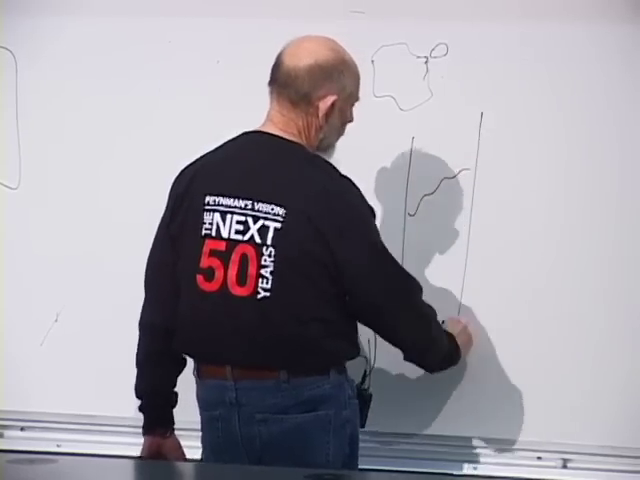
\includegraphics[width=0.72\textwidth]{lecture_06_figure_03.png}
\caption{칠판에 완성된 교환 그림. 방출과 흡수에 각각 결합 인자가 붙어 있다.}
\lectureframe{00:11:30.000}
\end{figure}

끈 이론에서는 광자가 중력자로, 전하가 \(g_s\)로 바뀐다. 방출에 하나, 흡수에 하나씩 인자가 붙으므로 중력의 세기는 \(g_s^2\)에 비례한다.

먼 거리에 있는 같은 상호작용은 뉴턴의 힘 법칙을 재현해야 한다.
\begin{equation}
F_{\mathrm{grav}}\sim G_N\frac{M_1M_2}{r^2}.
\end{equation}
질량과 역제곱 의존성은 원천과 전파를 나타낸다. 여기서 필요한 점은 그 항들에 곱해지는 결합이다.

\begin{figure}[htbp]
\centering
\begin{tikzpicture}[x=1cm,y=1cm]
  \node[font=\small\bfseries] at (1.8,3.55) {electromagnetism};
  \draw[line width=0.8pt] (0,0) -- (0,3);
  \draw[line width=0.8pt] (3.6,0) -- (3.6,3);
  \draw[line width=0.8pt] plot[smooth] coordinates {(0,1.5) (0.45,1.72) (0.9,1.28) (1.35,1.72) (1.8,1.28) (2.25,1.72) (2.7,1.28) (3.15,1.72) (3.6,1.5)};
  \node[below] at (0,1.42) {\(e\)};
  \node[below] at (3.6,1.42) {\(e\)};
  \node[font=\small] at (1.8,0.25) {exchange strength \(\propto e^2\)};
  \node[font=\small\bfseries] at (7.2,3.55) {string gravity};
  \draw[line width=0.8pt,rounded corners=6pt] (5.4,0) -- (5.2,0.7) -- (5.5,1.5) -- (5.25,2.3) -- (5.4,3);
  \draw[line width=0.8pt,rounded corners=6pt] (9,0) -- (9.2,0.7) -- (8.9,1.5) -- (9.15,2.3) -- (9,3);
  \draw[line width=0.8pt] plot[smooth] coordinates {(5.5,1.5) (5.95,1.72) (6.4,1.28) (6.85,1.72) (7.3,1.28) (7.75,1.72) (8.2,1.28) (8.65,1.72) (8.9,1.5)};
  \node[below] at (5.5,1.42) {\(g_s\)};
  \node[below] at (8.9,1.42) {\(g_s\)};
  \node[font=\small] at (7.2,0.25) {exchange strength \(\propto g_s^2\)};
\end{tikzpicture}
\caption{결합을 세는 비유. 교환되는 양자의 양 끝에서 각각 하나의 상호작용 인자가 기여한다.}
\end{figure}

이 관찰로 뉴턴 상수를 거의 결정할 수 있다. 결합 \(g_s\)는 무차원인 반면, 4차원에서 \(G_N\)의 차원은 길이의 제곱이다. 쓸 수 있는 미시적 길이는 \(\ell_s\)이므로,
\begin{equation}
G_N\sim g_s^2\ell_s^2.
\label{eq:l06-newton-string}
\end{equation}
이를 식~\eqref{eq:l06-planck-area}과 결합하면 다음을 얻는다.
\begin{equation}
\ell_p\sim g_s\ell_s.
\label{eq:l06-planck-string}
\end{equation}

\begin{figure}[htbp]
\centering
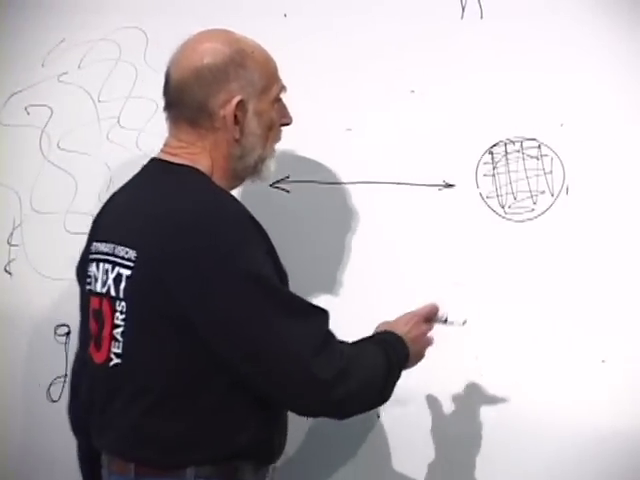
\includegraphics[width=0.72\textwidth]{lecture_06_figure_04.png}
\caption{칠판에 남겨 둔 기본 관계식: \(\ell_p^2=G_N\)와 \(\ell_p\sim g_s\ell_s\).}
\lectureframe{00:15:45.000}
\end{figure}

식~\eqref{eq:l06-newton-string}은 이 강의 전반에서 사용하는 단순화된 관계식이다.\editorialnote{콤팩트화된 끈 이론에서 유효한 4차원 뉴턴 상수는 콤팩트화 부피와 1 정도 크기의 관례에도 의존한다. 강의에서는 대응 관계의 스케일링에 초점을 맞추기 위해 그 정보를 생략한다.}

\begin{classroomqa}
\audiencequestion{\(g_s\)은 1보다 큰가요, 작은가요? 또 어느 길이가 더 큰가요?\lecturetimestamp{00:16:00}}
\lecturerresponse{결합이 약한 영역인 \(g_s<1\)에서 다룹니다. 그러면 \(\ell_p\sim g_s\ell_s\)에 따라 끈 길이가 플랑크 길이보다 큽니다. 강결합에서는 다른 기술이 필요하지만, 여기서는 다루지 않아도 됩니다.}
\end{classroomqa}

\section{블랙홀의 상태 수}

볼츠만 상수와 수치 인자를 생략하면 베켄슈타인--호킹 엔트로피는 다음과 같다.
\begin{equation}
S_{\mathrm{BH}}=\frac{A}{4G_N}sim\frac{A}{G_N}sim\frac{A}{\ell_p^2}.
\label{eq:l06-bh-area}
\end{equation}
반고전적 공식에서 \(1/4\) 인자는 정확한 값이지만, 이 스케일링 논증에서는 아무 역할도 하지 않는다.

\begin{classroomqa}
\audiencequestion{아래 첨자 ``BH''는 블랙홀을 뜻하나요, 베켄슈타인--호킹을 뜻하나요?\lecturetimestamp{00:16:51}}
\lecturerresponse{우리에게는 둘 다 떠올리게 하는 표기로 보면 됩니다. 핵심은 엔트로피가 플랑크 면적 단위로 잰 사건의 지평선 면적이라는 점입니다.}
\end{classroomqa}

4차원 슈바르츠실트 블랙홀의 경우,
\begin{equation}
R_s=2G_NM,
\qquad
A=4\pi R_s^2.
\end{equation}
강의에서처럼 \(2\)와 \(4\pi\)를 생략하면,
\begin{align}
S_{\mathrm{BH}}
&\sim \frac{R_s^2}{G_N}
\sim \frac{(G_NM)^2}{G_N} \\
&\sim M^2G_N
\sim M^2\ell_p^2.
\label{eq:l06-bh-mass}
\end{align}
이 형태를 끈의 상태 수와 비교할 것이다.

\section{랜덤 워크로 보는 긴 끈}

작은 끈에서 시작해 에너지를 주입하자. 일반적인 고도로 들뜬 끈은 단정한 고리 모양으로 남아 있지 않는다. 감긴 낚싯줄을 잘못 풀었을 때처럼 길고 복잡하게 얽힌 물체가 된다. 거시적으로는 서로 구별되지 않는 배치가 매우 많기 때문에 이 얽힌 끈에는 엔트로피가 있다.

상태 수를 세기 위해 공간을 링크의 길이가 \(\ell_s\)인 격자로 바꿔 생각하자. 꼭짓점은 격자점이고 선은 링크이며, 기본 정사각형은 면이다. 끈은 연결된 링크들의 연속으로 나타낸다. 이 모형은 의도적으로 거칠게 단순화했지만, 상태 수의 지수적 증가는 원하는 스케일링을 포착한다.

\begin{figure}[htbp]
\centering
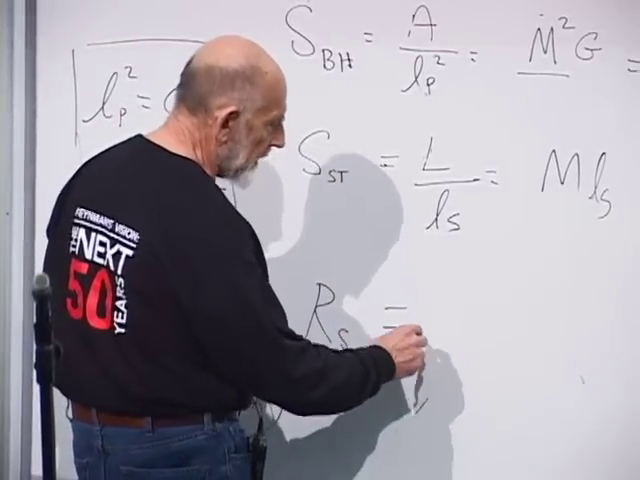
\includegraphics[width=0.72\textwidth]{lecture_06_figure_05.png}
\caption{2차원 격자 모형. 파란 선분은 끈의 한 걸음을 나타내며, 각 격자점에서 가능한 네 가지 다음 경로를 센다.}
\lectureframe{00:23:50.000}
\end{figure}

\begin{classroomqa}
\audiencequestion{이 단순한 워크에서는 매 단계마다 몇 가지 선택지가 있나요?\lecturetimestamp{00:22:43}}
\lecturerresponse{제곱 격자에서는 네 가지입니다. 바로 되돌아가는 경로도 허용하기 때문입니다. 3차원에서는 여섯 가지가 됩니다. 다른 격자를 쓰면 보통의 수는 달라지지만, 링크 수가 늘어남에 따라 워크 수가 지수적으로 증가한다는 점은 변하지 않습니다.}
\end{classroomqa}

끈에 \(n\)개의 링크가 있으면, 2차원 단순 모형에서 상태 수는 다음과 같다.
\begin{equation}
\Omega_n\sim4^n.
\label{eq:l06-walk-count}
\end{equation}
예외적으로 곧게 뻗은 워크 하나가 있지만, 이는 \(4^n\)개 상태 가운데 하나에 불과하다. 전형적인 워크는 여러 차례 접히며 얽힌 덩어리를 이룬다. \(n\)가 크면 무작위로 만든 거의 모든 배치는 질적으로 서로 비슷해 보인다.

거시적으로 구별할 수 없는 배치의 수에 로그를 취하면 엔트로피가 된다.
\begin{equation}
S_{\mathrm{st}}=\log\Omega_n\sim n\log4\sim n.
\label{eq:l06-string-entropy-n}
\end{equation}

\begin{classroomqa}
\audiencequestion{왜 엔트로피는 \(4^n\)이 아니라 \(n\)에 비례하게 되나요?\lecturetimestamp{00:25:39}}
\lecturerresponse{엔트로피는 상태 수의 로그입니다. 따라서 \(\log(4^n)=n\log4\)이고, 인자 \(\log4\)은 1 정도의 상수이므로 생략하겠습니다.}
\end{classroomqa}

끈의 한쪽 끝에서 다른 쪽 끝까지 따라가며 잰 윤곽 길이가 \(L\)라면,
\begin{equation}
n=\frac{L}{\ell_s},
\qquad
S_{\mathrm{st}}\sim\frac{L}{\ell_s}.
\label{eq:l06-string-entropy-length}
\end{equation}
여기서 \(L\)는 얽힌 덩어리의 지름이 아니다. 끈을 따라 잰 훨씬 더 긴 거리다.

이제 윤곽 길이를 질량으로 바꾸자. \(c=\hbar=1\)에서는 질량의 차원이 길이의 역수다. 따라서 끈 길이 하나에 해당하는 링크 하나의 질량은 대략
\begin{equation}
m_{\mathrm{link}}\sim\frac{1}{\ell_s}.
\label{eq:l06-link-mass}
\end{equation}

\begin{classroomqa}
\audiencequestion{링크 하나의 질량이 왜 \(1/\ell_s\)에 비례해야 하나요?\lecturetimestamp{00:29:20}}
\lecturerresponse{이 단위계에서 질량은 길이의 역수이고, 쓸 수 있는 유일한 길이는 \(\ell_s\)입니다. 달리 말해, \(1/\ell_s^2\) 정도의 끈 장력에 링크 길이 \(\ell_s\)를 곱해도 같은 결과를 얻습니다.}
\end{classroomqa}

그러면 끈 전체의 질량은
\begin{equation}
M\sim n m_{\mathrm{link}}
\sim\frac{n}{\ell_s}
\sim\frac{L}{\ell_s^2},
\qquad
L\sim M\ell_s^2.
\label{eq:l06-string-mass}
\end{equation}
식~\eqref{eq:l06-string-entropy-length}에 대입하면 다음을 얻는다.
\begin{equation}
S_{\mathrm{st}}\sim M\ell_s.
\label{eq:l06-string-entropy-mass}
\end{equation}
격자 워크는 월드시트 제약 조건과 수치 계수를 무시하지만, 고도로 들뜬 끈 스펙트럼의 지수적 증가는 이와 같은 선도 스케일링을 준다.\editorialnote{랜덤 워크 구성은 끈 상태의 높은 준위 밀도를 기억하기 위한 도식일 뿐, 기본 끈을 실제로 이산화한 것은 아니다.}

\section{논증의 출발점이 되는 불일치}

이제 두 결과를 나란히 놓으면 다음과 같다.
\begin{equation}
S_{\mathrm{BH}}\sim M^2\ell_p^2,
\qquad
S_{\mathrm{st}}\sim M\ell_s.
\label{eq:l06-two-entropies}
\end{equation}
두 식은 서로 비슷해 보이지만, 질량을 고정하고 결합을 임의로 택하면 같지 않다. 블랙홀 식은 \(M\)의 제곱에 비례하고, 끈 식은 선형으로 비례한다. 뜨거운 끈을 아무 설명 없이 블랙홀이라고 선언할 수는 없다. 두 영역이 어떻게 이어지는지 밝혀야 한다.

\begin{figure}[htbp]
\centering
\includegraphics[width=0.78\textwidth]{lecture_06_figure_06.png}
\caption{가림 없이 칠판에 나란히 적은 비교: 위에는 블랙홀 엔트로피, 아래에는 긴 끈 엔트로피가 있고, 왼쪽에는 플랑크--끈 관계식이 남아 있다.}
\lectureframe{00:33:20.000}
\end{figure}

여기서 강의는 잠시 멈춘다. 긴장감을 남기는 것은 유익하다. 이 불일치는 발상이 틀렸다는 뜻이 아니라, 중력의 세기를 바꾸면서 동일한 상태를 비교해야 한다는 단서다.

\section{결합의 조절 손잡이를 돌리기}

\(\ell_s\)를 고정하고 \(g_s\)를 바꿀 수 있다고 생각해 보자. \(g_s=0\)에서는 끈이 분리되거나 결합하지 않으며, \(G_N\sim g_s^2\ell_s^2\)이므로 중력도 사라진다. 따라서 에너지가 충분히 큰 상태는 길고 상호작용이 약한 끈이다.

\(g_s\)를 천천히 키우자. 끈 상호작용이 가능해지고, 지금 논증에서 더 중요한 것은 중력이 강해진다는 점이다.

\begin{classroomqa}
\audiencequestion{\(g_s\)를 키우면, 가장 먼저 끈이 짧은 끈들로 갈라지기만 하나요?\lecturetimestamp{00:36:29}}
\lecturerresponse{분리와 결합이 가능해지지만, \(\ell_s\)를 고정하고 엔트로피가 높은 상태를 따라가 봅시다. 핵심 효과는 \(G_N\)가 커져 긴 끈의 자기중력이 얽힌 덩어리를 안쪽으로 끌어당기는 것입니다.}
\end{classroomqa}

물체는 수축하며 밀도가 높아진다. 중력 퍼텐셜 에너지는 음수이므로, 수축하면 총에너지가 낮아지고 따라서 질량도 감소한다.

\begin{classroomqa}
\audiencequestion{자기중력이 끈을 끌어당길 때 에너지는 증가하나요, 감소하나요?\lecturetimestamp{00:37:48}}
\lecturerresponse{감소합니다. 결합 에너지는 더 음수가 됩니다. 같은 상태를 계속 따라가더라도 그 경로를 따라 질량이 일정할 필요는 없습니다.}
\end{classroomqa}

결국 물체의 크기는 슈바르츠실트 반지름과 비슷해진다. 그 지점을 지나면 블랙홀로 기술하는 것이 자연스럽다. 초기 들뜸이 클수록 더 작은 결합에서 이 조건에 도달한다. 질량이 큰 물체일수록 사건의 지평선을 만들기 위해 필요한 중력의 세기가 더 약하기 때문이다.

\begin{figure}[htbp]
\centering
\resizebox{0.95\linewidth}{!}{%
\begin{tikzpicture}[x=1cm,y=1cm,>=Latex]
  \draw[->,line width=0.9pt] (0,0) -- (11,0) node[right] {increasing \(g_s\)};
  \node[draw,rounded corners,align=center,minimum width=2.6cm,minimum height=1.15cm] at (1.8,1.5) {long excited string\\weak self-gravity};
  \node[draw,rounded corners,align=center,minimum width=2.6cm,minimum height=1.15cm] at (5.5,1.5) {correspondence point\\\(R_s\sim\ell_s\)};
  \node[draw,circle,align=center,minimum size=1.8cm] at (9.3,1.5) {black\\hole};
  \draw[->,line width=0.8pt] (3.15,1.5) -- (4.1,1.5) node[midway,above,font=\small] {contracts};
  \draw[->,line width=0.8pt] (6.9,1.5) -- (8.25,1.5);
  \node[font=\small,align=center] at (5.5,-0.65) {same family of states followed slowly;\\binding energy and mass may change};
\end{tikzpicture}
}
\caption{\(\ell_s\)를 고정한 대응 경로. 화살표를 거꾸로 따라가면 블랙홀 상태가 긴 끈 상태로 돌아간다.}
\end{figure}

\begin{classroomqa}
\audiencequestion{\(g_s\)가 0과 1 사이에 있다고 생각하면 되나요?\lecturetimestamp{00:40:18}}
\lecturerresponse{그렇습니다. 논증은 약결합 영역에서 이루어집니다. \(g_s\)가 매우 작으면 상태가 블랙홀이 되려면 그에 맞게 질량이 커야 합니다. 제어가 어려운 \(g_s>1\) 영역에 들어갈 필요는 없습니다.}
\end{classroomqa}

이 사고실험에서 느린 변화는 가역적이다.

\begin{classroomqa}
\audiencequestion{중력이 블랙홀을 붙들어 두지 못할 때까지 결합을 다시 낮추면, 블랙홀은 무엇이 되나요?\lecturetimestamp{00:41:37}}
\lecturerresponse{긴 끈이 됩니다. 이 구성에서 중력이 사라지면 모든 것은 끈 상태로 기술되어야 합니다. 조절 손잡이를 한쪽으로 돌리면 끈이 블랙홀이 되고, 반대로 돌리면 블랙홀이 끈이 됩니다.}
\end{classroomqa}

총에너지와 부피를 고정하면, 엔트로피가 가장 큰 배치는 짧은 끈이 엄청나게 많은 상태라기보다 사실상 긴 끈 하나다. 이 명제는 여기서 유도하지 않는다. 하게도 영역에 가까운 끈의 통계역학에서 나오는 결과이며, 뒤에서 다시 다룬다.

\section{외부 관찰자가 보는 것}

물체가 블랙홀로 기술될 때 끈은 어디에 있는가? 외부 관찰자의 기술에서는 끈이 갑자기 사라지지 않는다. 슈바르츠실트 시간으로 보면 겉보기에는 사건의 지평선을 통과하는 시각이 무한히 늦어지므로, 끈의 자유도는 지평선 위나 그 근처에 쌓이는 것으로 나타난다.

\begin{figure}[htbp]
\centering
\includegraphics[width=0.72\textwidth]{lecture_06_figure_07.png}
\caption{거시적 지평선에서는 끈 길이 척도의 구조가 얇은 흐림층처럼 보이는 반면, 반지름이 고리 척도에 가까운 작은 지평선에서는 그 구조가 어떻게 보이는지 칠판에 비교해 그렸다.}
\lectureframe{00:45:30.000}
\end{figure}

\(R_s\gg\ell_s\)일 때 블랙홀은 거시적이며, 지평선 반지름에 비하면 끈 길이 척도의 구조는 얇은 층에 불과하다. 반지름이 \(\ell_s\)에 가까워지면 매끄러운 블랙홀과 늘어난 끈의 구분은 의미를 잃는다. 이것은 외부 관찰자의 늘어난 지평선 기술이다. 낙하하는 물질이 정칙한 지평선을 결코 통과하지 않는다는 좌표 독립적 주장과 혼동해서는 안 된다.\editorialnote{강의에서는 블랙홀 상보성에서 익숙한 외부 영역의 기술을 사용한다. 지평선``위''라는 표현은 외부 관찰자의 기술로 분해해 볼 수 있는 자유도를 가리키며, 그 자유도의 공변적인 위치를 따로 유도했다는 뜻은 아니다.}

전이는 다음 조건에서 일어난다.
\begin{equation}
R_s\sim\ell_s.
\label{eq:l06-correspondence-radius}
\end{equation}
끈 척도보다 작은 영역에서는 슈바르츠실트 기하가 블랙홀을 지탱한다고 여겨지는 구조를 분해해 볼 수 없다. 고리들은 예상되는 지평선에서 벗어나 요동하므로, 그 상태는 끈이라고 부르는 편이 더 적절하다.

\section{대응점}

식~\eqref{eq:l06-correspondence-radius}에 \(R_s\sim G_NM\)를 사용하면,
\begin{equation}
G_NM\sim\ell_s.
\end{equation}
그다음 \(G_N\sim g_s^2\ell_s^2\)를 대입하면,
\begin{equation}
M g_s^2\ell_s^2\sim\ell_s,
\qquad
M g_s^2\ell_s\sim1.
\label{eq:l06-correspondence-condition}
\end{equation}

\begin{figure}[htbp]
\centering
\includegraphics[width=0.72\textwidth]{lecture_06_figure_08.png}
\caption{칠판에 완성한 전이 계산: \(R_s\sim\ell_s\)에서 상자 안의 무차원 조건 \(Mg_s^2\ell_s\sim1\)을 얻는다.}
\lectureframe{00:49:50.000}
\end{figure}

청중 가운데 한 사람이 이 조건이 무엇을 예고하는지 알아차렸다. 대응점에서는
\begin{align}
S_{\mathrm{BH}}
&\sim M^2\ell_p^2
\sim M^2g_s^2\ell_s^2 \\
&=(M\ell_s)(Mg_s^2\ell_s)
\sim M\ell_s
\sim S_{\mathrm{st}}.
\label{eq:l06-entropy-preview}
\end{align}

\begin{classroomqa}
\audiencequestion{이 방정식들은 블랙홀 엔트로피와 끈 엔트로피가 같아짐을 이미 함의하나요?\lecturetimestamp{00:50:18}}
\lecturerresponse{그렇습니다. 계산이 바로 그 결론으로 향하고 있습니다. 필요한 재료는 칠판에 나와 있지만, 대응 관계의 논리를 차근차근 다시 살펴볼 수 있도록 강의에서는 이 재료들을 완전히 결합하는 일을 뒤로 미룹니다.}
\end{classroomqa}

식~\eqref{eq:l06-entropy-preview}은 문답에서 암묵적으로 예고된 한 줄짜리 대수 계산이다. 이는 스케일링을 확립하지만 정확한 계수 \(1/4\)까지 정하지는 않는다. 정확한 미시적 일치를 얻으려면 더 통제 가능한 블랙홀과 더 상세한 끈 구성이 필요하다.\editorialnote{강의는 식~\eqref{eq:l06-entropy-preview}을 완성된 유도로 제시하기 전에 끝난다. 청중이 등식을 분명히 짚었고 필요한 관계식이 모두 앞서 나왔으므로, 여기에는 식을 명시해 두었다.}

\section{엔트로피를 보존할 수 있는 이유}

마지막으로 논리적 요소 하나가 남아 있다. 계가 고립되어 있고 변화가 가역적일 때, 자기장이나 \(g_s\) 같은 제어 매개변수를 충분히 천천히 바꾼다고 하자. 에너지, 크기, 결합 에너지는 달라질 수 있지만 엔트로피는 보존된다.
\begin{equation}
\Delta S=0.
\label{eq:l06-adiabatic-entropy}
\end{equation}
강의에서는 이를 정보 보존과 연결한다. 엔트로피는 거친 눈금의 기술에 가려진 정보를 측정한다. 해밀토니안을 천천히 가역적으로 바꾸면 그 정보는 없어지지 않고 상태들이 재배열된다.

\begin{classroomqa}
\audiencequestion{엔트로피를 일정하게 유지하려면 경로가 상전이를 피해야 하나요?\lecturetimestamp{00:54:01}}
\lecturerresponse{그렇습니다. 상태를 연속적으로 따라갈 수 있어야 합니다. 유한한 계에는 무한 부피계와 같은 의미에서 비해석적인 열역학적 상전이가 엄밀히 존재하지 않습니다. 변화가 충분히 느리면 대응 관계를 매끄러운 교차로 다룰 수 있습니다.}
\end{classroomqa}

여기서 단열은 더 강한 의미인 준정적이고 가역적인 과정으로 사용된다. 단열이더라도 비가역 과정에서는 엔트로피가 생성될 수 있다. 느린 변화와 상태를 추적할 수 있다는 점이 핵심이다.\editorialnote{열역학적 명제 \(\Delta S=0\)에는 가역 단열 경로가 필요하다. 양자역학적으로 이에 대응하는 생각은 매개변수가 변하는 동안 제어되지 않은 준위 전이가 일어나지 않게 하면서 동일한 상태 집합을 따라가는 것이다.}

\begin{classroomqa}
\audiencequestion{같은 총질량을 지닌 짧은 끈 여러 개보다 긴 끈 하나의 엔트로피가 더 큰 이유는 무엇인가요?\lecturetimestamp{00:54:44}}
\lecturerresponse{직관에 어긋나지만, 유한한 부피에서 고에너지 상태 수를 직접 세어 보면 긴 끈 성분이 우세합니다. 증명은 뒤로 미룬다. 지금 논증에 필요한 것은 블랙홀이 매우 많은 짧은 끈으로 이루어진 희박한 기체가 아니라 최대 엔트로피 끈 부문으로 대응한다는 점뿐이다.}
\end{classroomqa}

따라서 실제로 따를 전략은 다음과 같다.
\begin{enumerate}
\item \(M_0\)의 질량과 \(g_{s,0}\)의 결합을 가진 블랙홀에서 시작한다.
\item \(g_s\)를 천천히 낮추면서 엔트로피가 높은 동일한 상태 계열을 따라간다.
\item \(R_s\sim\ell_s\)에서 멈춘다. 이 지점에서는 블랙홀 기술이 긴 끈 기술로 바뀐다.
\item \(S_{\mathrm{st}}\sim M\ell_s\)를 사용해 끈 상태 수를 센다.
\item 그 엔트로피를 가역 경로를 따라 원래 블랙홀까지 보존한다.
\end{enumerate}

\begin{figure}[htbp]
\centering
\includegraphics[width=0.72\textwidth]{lecture_06_figure_09.png}
\caption{전략을 설명하는 동안 칠판에 남겨 둔 원리: \(g_s\)의 단열 변화는 \(S\)를 바꾸지 않는다.}
\lectureframe{00:56:40.000}
\end{figure}

끈 이론은 전하를 띠거나 회전하는 블랙홀, 초대칭 블랙홀, 극한에 가까운 블랙홀, 고차원 블랙홀의 엔트로피를 훨씬 정밀하게 셈해 왔다. 여기서 다룬 중성 슈바르츠실트 블랙홀은 거친 대응 논증으로, 상태 밀도의 매개변수 의존성과 물리적 교차를 밝힐 뿐 보호된 축퇴도의 정확한 값을 구하지는 않는다.\editorialnote{결합이 변해도 상태 수가 보호되는 특별한 블랙홀에서 정확한 일치가 가장 잘 성립한다. 이 강의에서는 의도적으로 가장 단순한 크기 정도의 계산을 제시한다.}

\begin{classroomqa}
\audiencequestion{중력을 끄면 상태가 끈 하나로 정확히 이루어지는 대신 끈 두 개로 이루어질 수도 있나요?\lecturetimestamp{00:58:25}}
\lecturerresponse{긴 끈이 소수만 존재할 확률은 유한하며, 끈 하나 대신 둘을 사용해도 엔트로피의 선도적 스케일링은 달라지지 않습니다. 논증을 바꾸게 될 것은 짧은 끈으로 이루어진 거대한 기체로의 분열이지만, 고에너지 통계적 계수는 그런 결과를 선호하지 않습니다.}
\end{classroomqa}

블랙홀은 한 영역 안에 담을 수 있는 엔트로피가 가장 큰 상태이며, 중력을 제거했을 때 이에 대응하는 고엔트로피 상태는 긴 끈이다. 이제 두 기술은 연결되었지만, 아직 정밀한 계산으로 발전하지는 않았다. 다음 단계에서는 대수 계산을 꼼꼼히 반복하고 이 대응 관계를 어디까지 신뢰할 수 있는지 살펴본다.

\chapter{블랙홀 엔트로피, 홀로그래피, 드시터르 공간}

\lectureoverview{앞선 강의에서 시작한 대응 논증을 마무리한다. 고도로 여기된 끈의 엔트로피는 질량에 비례하는 반면, 슈바르츠실트 블랙홀의 엔트로피는 면적에 비례한다. 두 식은 강한 중력장을 가진 블랙홀을 자유 끈과 동일시해서 연결되는 것이 아니라, 끈 결합상수를 천천히 변화시켜 두 기술 방식이 만나는 지점에 이르러 연결된다. 그러면 면적 법칙은 자연스럽게 홀로그래피 원리로 이어진다. 강의의 마지막 부분에서는 팽창하는 공간과 드시터르 기하를 소개한다. 그 지평선은 다음 강의에서 살펴본다.}

\section{계수 문제로 돌아가기}

긴 끈의 개수를 셀 때 아직 매듭짓지 않은 문제가 하나 있었다. 고정된 총길이를 여러 끈에 나누어 배정하면, 길이가 같은 동일한 끈들은 서로 구별되지 않는다. 하지만 상자 안에서 끈이 차지하는 위치는 상태의 일부이며, 상자의 크기는 해당하는 하나의 긴 끈이 차지하는 영역과 대략 같게 정한다.

\begin{classroomqa}
\audiencequestion{짧은 끈들은 서로 구별되는가? 끈들의 위치도 계산에 포함되는가?\lecturetimestamp{00:00:37}}
\lecturerresponse{성질이 동일한 끈들은 서로 구별되지 않지만, 상자 안에서 끈들이 차지하는 위치는 계산에 포함한다. 부피를 고정한 채 비교하며, 그 부피는 긴 끈이 차지하는 영역과 같게 정한다.}
\end{classroomqa}

이 문제를 정리했으니 이제 목표를 말할 수 있다. 몇 가지 방정식을 모아 블랙홀 엔트로피의 스케일링을 구할 것이다. 적분이나 무한합은 필요하지 않다. 어려움은 대수 계산에 있지 않다. 어떤 양들을 서로 비교할 수 있는지, 논증의 어느 단계에서 비교해야 하는지를 아는 데 있다.

\section{자연 단위계와 플랑크 면적}

다음과 같이 두되
\begin{equation}
c=\hbar=1,
\label{eq:l07-natural-units}
\end{equation}
뉴턴 상수는 명시적으로 남겨 둔다. 우선 시간과 길이의 단위가 같아진다. 광자 관계식
\begin{equation}
E=\frac{\hbar c}{\lambda}
\end{equation}
과 질량-에너지 관계식 \(E=mc^2\)에서 다음을 얻는다.
\begin{equation}
[M]=L^{-1}.
\label{eq:l07-mass-dimension}
\end{equation}
따라서 질량은 역길이 단위로 나타낼 수 있다.

\begin{figure}[htbp]
\centering
\includegraphics[width=0.62\textwidth]{lecture_07_figure_02.png}
\caption{차원 논증을 시작할 때 사용하는 자연 단위계 관례. 에너지 식은 위 방정식들에서 완성된다.}
\lectureframe{00:03:27.900}
\end{figure}

\(G_N\)의 단위를 정하려면 뉴턴 역학의 가속도를 차원 계산에만 사용한다.
\begin{equation}
a\sim\frac{G_NM}{R^2}.
\end{equation}
\(T\)과 \(L\)의 단위가 같으므로 \([a]=L/T^2=L^{-1}\)이다. 이를 식~\eqref{eq:l07-mass-dimension}과 함께 사용하면 다음을 얻는다.
\begin{equation}
[G_N]=L^2.
\end{equation}
이 단위계에서 뉴턴 상수는 면적이다. 플랑크 길이를
\begin{equation}
G_N=\ell_p^2,
\label{eq:l07-planck-area}
\end{equation}
로 정의하면, \(A/G_N=A/\ell_p^2\)가 무차원인 이유를 곧바로 알 수 있다. 이는 플랑크 면적 단위로 면적을 잰 값이다.

\section{끈 결합상수와 중력의 세기}

이제 중력을 끈 이론의 언어로 바꾸어야 한다. 유용한 그림은 교환 과정이다. 끈이 자기 자신과 교차할 때 분열한 뒤 다시 결합할 수 있다. 한 물체가 작은 닫힌 끈 고리를 방출하고 다른 물체가 이를 흡수할 수 있다. 그 들뜸이 중력자라면 이 과정이 중력을 매개한다. 방출 때 한 번, 흡수 때 한 번 상호작용 인자가 나타나므로 교환 세기에는 \(g_s^2\)가 포함된다.

결합상수 \(g_s\)는 무차원이다. 더 정확히 말하면 진폭 수준의 결합상수이며, 확률이나 율은 \(g_s^2\) 차수에서 시작한다.\editorialnote{강의에서는 때때로 \(g_s\)를 확률이라고 부른 뒤 확률의 제곱근이라고 정정한다. 섭동 결합상수는 진폭 수준의 양이다.} \(G_N\)은 면적의 차원을 가지므로 길이 척도가 여전히 필요하다. 기본 끈 길이 \(\ell_s\)는 기본적인 끈 요동 하나의 척도이며, 필요한 길이 척도를 제공한다.
\begin{equation}
G_N\sim g_s^2\ell_s^2,
\qquad
\ell_p\sim g_s\ell_s.
\label{eq:l07-planck-string}
\end{equation}

\begin{figure}[htbp]
\centering
\includegraphics[width=0.72\textwidth]{lecture_07_figure_05.png}
\caption{칠판에 적힌 결합상수 관계: \(G_N=\ell_p^2\)와 \(g_s^2\ell_s^2\sim\ell_p^2\).}
\lectureframe{00:12:15.000}
\end{figure}

약한 결합에서 \(g_s\ll1\)이면 플랑크 길이는 끈 길이보다 훨씬 짧다. \(g_s\)를 낮추면 기본 끈의 척도는 고정한 채 중력이 약해진다.\editorialnote{유효 4차원 이론에서는 압축화 자료와 수치 관례도 \(G_N\)에 들어간다. 이 스케일링 논증에서는 이를 고정하고 생략한다.}

\section{긴 끈의 계수}

엔트로피는 상태를 지정하는 데 필요한 기본 선택의 수를 센다. 고도로 여기된 끈을 정사각 격자 위의 보행으로 바꾸어 생각해 보자. 각 꼭짓점에서 다음 링크는 네 방향 가운데 하나를 향할 수 있다. 기본 선택을 네 가지 중 하나를 고르는 것으로 보든, 두 번의 이진 선택으로 보든 달라지는 것은 1 정도의 상수뿐이다. 중요한 것은 걸음의 수다.

\(L\)가 끈의 윤곽 길이이고 각 걸음의 길이가 \(\ell_s\)라면
\begin{equation}
N=\frac{L}{\ell_s}
\end{equation}
걸음이 필요하다. 보행의 수는 개략적으로 \(\Omega_N\sim q^N\)처럼 지수적으로 증가하며, \(q\)는 1 정도의 값이다. 따라서
\begin{equation}
S_{\mathrm{str}}=\log\Omega_N\sim N\sim\frac{L}{\ell_s}.
\label{eq:l07-string-entropy-length}
\end{equation}

\begin{figure}[htbp]
\centering
\includegraphics[width=0.68\textwidth]{lecture_07_figure_03.png}

\vspace{0.7em}
\begin{tikzpicture}[scale=0.82]
  \draw[step=0.8cm,gray!45,thin] (0,0) grid (6.4,4.0);
  \draw[very thick,blue!60!black]
    (0.8,0.8)--(1.6,0.8)--(1.6,1.6)--(2.4,1.6)--(2.4,2.4)--
    (3.2,2.4)--(3.2,1.6)--(4.0,1.6)--(4.0,2.4)--(4.8,2.4)--
    (4.8,3.2)--(5.6,3.2);
  \draw[<->,thick] (0.8,-0.35)--(1.6,-0.35);
  \node[below] at (1.2,-0.35) {step \(\ell_s\)};
  \node[align=center] at (8.1,2.0) {\(N=L/\ell_s\) steps\\[0.3em]\(S_{\mathrm{str}}\sim N\)};
\end{tikzpicture}
\caption{칠판의 격자 모형과 이를 정리한 무작위 보행 해석. 엉킨 공의 지름이 아니라 윤곽 길이가 선택의 수를 결정한다.}
\lectureframe{00:17:20.000}
\end{figure}

같은 기본 선분들로 질량을 센다. 길이 \(\ell_s\)인 선분의 질량 척도는
\begin{equation}
m_{\mathrm{seg}}\sim\frac{1}{\ell_s}.
\end{equation}

\begin{classroomqa}
\audiencequestion{기본 선분에 길이 \(\ell_s\)를 부여하는 건가요?\lecturetimestamp{00:18:56}}
\lecturerresponse{그렇다. 그 특성 길이는 \(\ell_s\)이므로 자연 단위계에서 특성 질량은 \(1/\ell_s\)이다.}
\end{classroomqa}

\(L/\ell_s\)개의 선분 질량을 더하면 다음과 같다.
\begin{equation}
M\sim\frac{L}{\ell_s}\frac{1}{\ell_s}
=\frac{L}{\ell_s^2},
\qquad
L\sim M\ell_s^2.
\label{eq:l07-string-mass}
\end{equation}
진동하는 끈의 운동에너지와 퍼텐셜 에너지는 이 스케일링 관계에 압축되어 있다. 상세한 통계역학적 처리를 해도 같은 의존성을 얻는다. 식~\eqref{eq:l07-string-entropy-length}에 대입하면 필요한 끈 이론의 식을 얻는다.
\begin{equation}
S_{\mathrm{str}}\sim M\ell_s.
\label{eq:l07-string-entropy-mass}
\end{equation}

\begin{figure}[htbp]
\centering
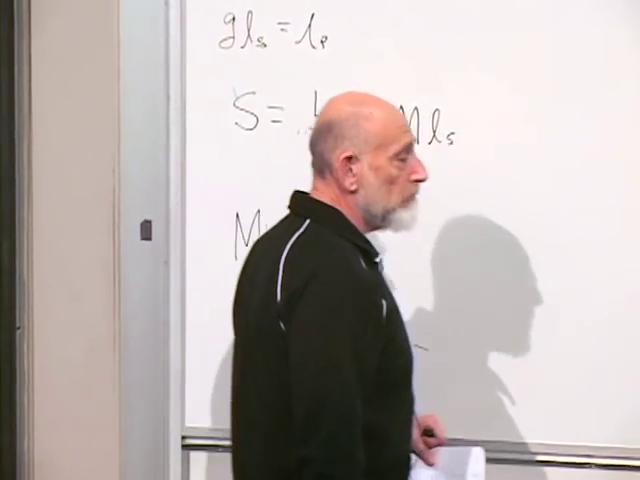
\includegraphics[width=0.66\textwidth]{lecture_07_figure_04.png}
\caption{비교에 앞서 정리한 끈 이론 쪽의 항목: \(\ell_p\sim g_s\ell_s\), \(S_{\mathrm{str}}\sim L/\ell_s\sim M\ell_s\), \(M\sim L/\ell_s^2\).}
\lectureframe{00:21:57.800}
\end{figure}

\section{자유 끈이 아직 블랙홀이 아닌 이유}

중력 쪽의 정확한 반고전적 공식은 다음과 같다.
\begin{equation}
S_{\mathrm{BH}}=\frac{A}{4G_N}.
\label{eq:l07-bh-exact}
\end{equation}

\begin{classroomqa}
\audiencequestion{분모에 들어가는 수치 계수는 얼마인가요?\lecturetimestamp{00:23:28}}
\lecturerresponse{4이다. 대응 논증으로 스케일링은 얻을 수 있지만, 이 논증은 너무 거칠어서 정확한 계수를 결정할 수 없다.}
\end{classroomqa}

4차원 슈바르츠실트 블랙홀에서는
\begin{equation}
R_s=2G_NM,
\qquad
A=4\pi R_s^2.
\end{equation}
강의에서처럼 수치 상수를 생략하면
\begin{align}
S_{\mathrm{BH}}
&\sim\frac{A}{G_N}
\sim\frac{(G_NM)^2}{G_N} \\
&\sim M^2G_N
\sim M^2\ell_p^2.
\label{eq:l07-bh-scaling}
\end{align}

\begin{figure}[htbp]
\centering
\includegraphics[width=0.72\textwidth]{lecture_07_figure_06.png}
\caption{칠판에서 완성한 비교: 끈 엔트로피는 끈 단위의 길이인 반면, 블랙홀 엔트로피는 플랑크 단위의 면적이다.}
\lectureframe{00:25:35.000}
\end{figure}

식~\eqref{eq:l07-string-entropy-mass}와 \eqref{eq:l07-bh-scaling}의 유사성은 시사하는 바가 있지만, 두 식은 같지 않다. 원래 블랙홀을 자유 끈이라고 부르고 대입하는 것은 잘못이다. 자유 끈의 계수에서는 끈을 이루는 부분들 사이의 인력이 빠져 있다. 바로 그 상호작용이 끈을 블랙홀 크기로 압축하고 음의 결합에너지를 통해 전체 에너지를 낮춘다.

별을 보면 이 오류가 익숙한 형태로 드러난다. 별의 질량을 가진 뜨거운 기체를 지나치게 큰 상자에 넣어 두는 것은 온도가 같더라도 별의 모형이 아니다. 자체 중력은 평형 크기와 에너지-엔트로피 관계를 바꾼다. 긴 끈의 모든 자체 상호작용을 따라가는 일은 어려우므로 그렇게 하지 않을 것이다.

\begin{classroomqa}
\audiencequestion{긴 끈에서 작은 고리가 떨어져 나가면 엔트로피가 감소합니다. 그렇다면 중력자 교환은 중력계의 엔트로피를 낮추나요?\lecturetimestamp{00:28:48}}
\lecturerresponse{여기서 다루는 평형 교환 과정에서는 그렇지 않다. 가상 들뜸은 양방향으로 방출되고 흡수된다. 이 그림은 끈 조각이 영구적으로 떨어져 나가는 실제 상황을 나타내지 않는다. 지금 이 그림의 목적은 결합상수 인자가 두 개 나타난다는 점과 그에 따라 \(g_s^2\) 의존성이 생긴다는 점만 보이는 것이다.}
\end{classroomqa}

\section{단열 대응 논증}

중력이 무시되는 조건에서 시작하자. \(g_s\to0\)일 때 끈들은 서로 지나쳐 가며 분열하거나 결합하지 않고, 자체 중력에 의한 인력도 사라진다. \(g_s\)를 높이면서 \(\ell_s\)는 고정하면 중력이 강해지고, 고도로 여기된 끈은 수축하다가 결국 블랙홀이 된다. 조절 변수를 천천히 되돌리면 블랙홀은 끈 상태로 돌아와야 한다. 긴 끈 몇 개가 될 수도 있지만, 앞선 강의의 고에너지 상태 수 계산에 따르면 지배적인 부문에는 짧은 끈으로 이루어진 엄청난 기체가 아니라 긴 끈 하나가 들어 있다.

\begin{classroomqa}
\audiencequestion{결합상수를 바꾸는 동안 무엇을 고정하나요?\lecturetimestamp{00:32:19}}
\lecturerresponse{끈 길이 \(\ell_s\), 따라서 기본 끈의 질량 척도 \(1/\ell_s\)를 고정한다. 조절 변수는 \(g_s\)를 바꾸고, 그에 따라 \(G_N\sim g_s^2\ell_s^2\)도 바뀐다.}
\end{classroomqa}

변화는 느리고 고립된 가역 과정이어야 한다. 이 조건에서는 엔트로피가 단열 불변량이다.
\begin{equation}
\Delta S=0.
\label{eq:l07-adiabatic}
\end{equation}
소산이나 통제되지 않은 천이가 일어난다면 느리게 변화시키는 것만으로는 충분하지 않다. 여기서 ``단열''이란 같은 상태들의 계열을 연속적으로 따라갈 수 있다는 뜻이다.\editorialnote{이는 가역적인 열역학 과정에서 말하는 단열의 의미다. 비가역 과정은 열의 출입이 없다는 의미에서는 단열이어도 엔트로피를 생성할 수 있다.}

목표 블랙홀의 질량을 \(M_0\), 결합상수를 \(g_{s,0}\)라고 하자. 설명하려는 면적 공식을 쓰기 전에 차원 분석으로 말할 수 있는 것은 중성 비회전 블랙홀의 엔트로피가 무차원 조합의 어떤 함수라는 점뿐이다.
\begin{equation}
S_{\mathrm{BH}}=f(M\ell_p)
=f(Mg_s\ell_s).
\label{eq:l07-entropy-function}
\end{equation}
\(\ell_s\)를 고정하면 등엔트로피 경로에서는 따라서 다음 양이 일정하게 유지된다.
\begin{equation}
Mg_s=M_0g_{s,0}
\label{eq:l07-adiabat}
\end{equation}
단, 같은 상태 가지를 따라간다고 가정한다.

\(g_s\)가 감소하면 음의 결합에너지가 제거되므로 이 경로를 따라 질량 \(M\)는 증가한다. 바탕이 되는 끈 구성도 결합이 느슨해져 퍼진다. 그러나 형식적인 슈바르츠실트 반지름은 단열 경로에서 \(R_s\sim Mg_s^2\ell_s^2\sim g_s\ell_s\)처럼 변하므로 감소한다.\editorialnote{구어 설명에서는 중력에 의한 결합에서 풀려난 물체에 대해 ``커진다''고 말한다. 이를 유도된 단열 경로를 따라 슈바르츠실트 반지름이 커진다는 뜻으로 받아들여서는 안 된다.}

\begin{classroomqa}
\audiencequestion{중력이 약해지면 물체는 커지나요, 작아지나요?\lecturetimestamp{00:36:28}}
\lecturerresponse{끈 구조는 결합에서 풀려나 팽창하고, 음의 결합에너지가 제거되므로 질량은 증가한다. 블랙홀 공식으로 정하는 반지름은 끈 척도에 이를 때까지 감소하며, 그 지점에서는 블랙홀 기술 방식이 더 이상 유용하지 않다.}
\end{classroomqa}

\section{두 곡선과 교점}

세로축에 질량, 가로축에 끈 결합상수를 놓고 그린다. 식~\eqref{eq:l07-adiabat}은 쌍곡선 \(M\propto g_s^{-1}\)이다.

\begin{classroomqa}
\audiencequestion{곱 \(Mg_s\)이 일정한 곡선은 어떤 모양인가요?\lecturetimestamp{00:44:08}}
\lecturerresponse{쌍곡선이다. 목표점 \((g_{s,0},M_0)\)을 지나는 단열 곡선이다.}
\end{classroomqa}

두 번째 곡선은 기술 방식이 바뀌는 교차 구간을 나타낸다. 블랙홀의 반지름이 기본 끈 요동의 크기보다 작아지면 이를 통상적인 슈바르츠실트 기하로 분해해 볼 수 없다. 따라서 대응점을 다음과 같이 추정한다.
\begin{equation}
R_s\sim\ell_s.
\label{eq:l07-correspondence-radius}
\end{equation}
\(R_s\sim MG_N\)와 식~\eqref{eq:l07-planck-string}을 사용하면 다음과 같다.
\begin{equation}
Mg_s^2\ell_s^2\sim\ell_s,
\qquad
Mg_s^2\sim\frac{1}{\ell_s}.
\label{eq:l07-transition-curve}
\end{equation}
따라서 전이 곡선은 \(M\propto g_s^{-2}\)에 따라 감소하며, 단열 곡선보다 더 가파르다.

\begin{figure}[htbp]
\centering
\includegraphics[width=0.70\textwidth]{lecture_07_figure_07.png}

\vspace{0.6em}
\begin{tikzpicture}[x=1cm,y=0.78cm]
  \draw[->] (0.4,0.4)--(7.0,0.4) node[right] {\(g_s\)};
  \draw[->] (0.4,0.4)--(0.4,6.5) node[above] {\(M\)};
  \draw[thick,black] plot[smooth] coordinates {(1.0,5.6) (1.5,4.0) (2.2,2.9) (3.2,2.1) (4.6,1.55) (6.3,1.2)};
  \draw[very thick,red!70!black] plot[smooth] coordinates {(1.25,6.0) (1.55,4.55) (2.0,3.15) (2.7,2.0) (3.8,1.25) (5.8,0.78)};
  \fill (2.05,3.1) circle (2pt) node[above right] {\((g_{s,*},M_*)\)};
  \node[black,rotate=-17] at (4.75,1.9) {\(Mg_s=M_0g_{s,0}\)};
  \node[red!70!black,rotate=-25] at (4.45,0.95) {\(Mg_s^2=1/\ell_s\)};
  \node at (5.75,3.5) {black hole};
  \node at (1.15,1.25) {string};
\end{tikzpicture}
\caption{칠판의 그래프와 이를 정리한 해석. 검은색 단열 곡선은 더 가파른 빨간색 대응 곡선과 교차한다. 그 교점에서 물체는 끈과 같은 성질을 띠게 된다.}
\lectureframe{00:49:35.000}
\end{figure}

교점 \((M_*,g_{s,*})\)에서는 두 방정식이 다음과 같다.
\begin{align}
M_*g_{s,*} &= M_0g_{s,0}, \\
M_*g_{s,*}^2 &\sim \frac{1}{\ell_s}.
\end{align}
첫 번째 방정식을 제곱하고 두 번째 방정식으로 나누면
\begin{equation}
M_*
\sim M_0^2g_{s,0}^2\ell_s.
\end{equation}
\(\ell_s\)를 곱하면
\begin{equation}
M_*\ell_s
\sim M_0^2g_{s,0}^2\ell_s^2
\sim M_0^2G_{N,0}.
\label{eq:l07-crossover-result}
\end{equation}

\begin{figure}[htbp]
\centering
\includegraphics[width=0.68\textwidth]{lecture_07_figure_08.png}
\caption{\(M_*\ell_s=M_0^2g_{s,0}^2\ell_s^2=M_0^2G_{N,0}\)를 포함해 완성한 교차 구간의 대수 계산.}
\lectureframe{00:54:40.000}
\end{figure}

\begin{classroomqa}
\audiencequestion{두 곡선의 방정식을 나눌 때 \(\ell_s\)는 분자의 위쪽에 오나요, 분모의 아래쪽에 오나요?\lecturetimestamp{00:52:41}}
\lecturerresponse{위쪽에 온다. \(1/\ell_s\)로 나누는 것은 \(\ell_s\)를 곱하는 것이므로 \(M_*\sim M_0^2g_{s,0}^2\ell_s\)가 된다.}
\end{classroomqa}

교차점에서는 끈 이론의 식이 유효하므로
\begin{equation}
S_*\sim M_*\ell_s.
\end{equation}
경로를 따라 엔트로피는 변하지 않았다. 이 사실을 식~\eqref{eq:l07-crossover-result}과 결합하면 원래 목표 블랙홀의 엔트로피를 얻는다.
\begin{equation}
S_{\mathrm{BH}}(M_0)
\sim M_0^2G_{N,0}
\sim M_0^2\ell_{p,0}^2.
\label{eq:l07-final-correspondence}
\end{equation}
이것이 원하는 면적 법칙의 스케일링이다.

\section{대응 논증이 증명하는 것과 증명하지 않는 것}

이 구성은 처음의 강한 중력장을 가진 블랙홀이 자유 끈이라고 말하지 않는다. 물체를 끈의 개수를 신뢰할 수 있는 영역으로 옮겨 그곳에서 엔트로피를 구한 다음, 그 엔트로피를 가역 경로를 따라 원래 상태로 되가져온다. 전이는 뚜렷한 상 경계가 아니라 크로스오버이므로, 이 추정으로는 계수 \(1/4\)를 식~\eqref{eq:l07-bh-exact}에서 정할 수 없다.

같은 논리는 전하를 띤 블랙홀, 다른 차원의 블랙 물체, 확장된 블랙 브레인에도 매개변수 의존성을 따지는 수준에서 성립한다. 대칭성이 더 크고 초대칭인 경우에는 결합상수가 변해도 보호되는 상태 계수를 통해 정확한 정보를 유지할 수 있다. 이런 방법은 수치 계수까지 얻지만, 여기서의 개념적 논증에는 필요하지 않은 수학적 장치를 더한다.

무엇보다 이 계산은 미시적 해석을 제공한다. 엔트로피는 숨겨진 구조의 증거다. 유체역학은 분자를 다루지 않고 밀도, 압력, 흐름을 기술하지만, 유체의 엔트로피는 그런 미시적 자유도가 있음을 드러낸다. 일반상대성이론도 마찬가지로 지평선을 기술하면서 그 미시상태를 보여 주지는 않는다. 끈 이론의 계수는 일관된 양자 중력 이론에 블랙홀 엔트로피를 설명할 만큼 충분한 상태가 들어 있을 수 있음을 보여 준다.

\begin{classroomqa}
\audiencequestion{\(S\sim M^3\ell_p^3\)대신 이런 세제곱 결과가 나왔다면 무엇을 뜻했을까요?\lecturetimestamp{00:59:41}}
\lecturerresponse{부피 법칙과 같은 형태였을 것이다. 방 안의 보통 물질이나 커피 한 잔의 엔트로피는 부피에 비례한다. 이차식의 답이 특별한 까닭은 \(R_s\sim M\ell_p^2\)을 통해 지평선 면적에 비례하기 때문이다.}
\end{classroomqa}

이 결과는 베켄슈타인--호킹 엔트로피가 단지 형식적인 열역학적 비유에 그치지 않는다는 증거다. 기본적인 유도 과정에서 중력의 자유도가 하나씩 눈에 보이게 드러나지는 않지만, 이 결과는 미시적인 중력 자유도가 있음을 가리킨다.

\section{최대 엔트로피에서 홀로그래피까지}

이제 질문을 바꾸자. 주어진 상태의 엔트로피를 묻는 대신, 어떤 영역에서 가능한 엔트로피의 최댓값을 묻는다.

방의 보통 격자 모형에서 시작하자. 부피를 크기 \(V_{\mathrm{cell}}\)의 셀들로 나누고, 각 셀에 점유 또는 비점유라는 예-아니요 선택 하나를 부여한다. Susskind는 실제 원자의 세부 사항이 계수에서 주의를 흐리지 않도록 가상의 원자에 일부러 우스꽝스러운 이름인 ``미토늄''을 붙인다. 만약
\begin{equation}
N=\frac{V}{V_{\mathrm{cell}}},
\end{equation}
이라면 구성의 수와 최대 엔트로피는 다음과 같다.
\begin{equation}
\Omega=2^N,
\qquad
S_{\max}=\log\Omega=N\log2
\sim\frac{V}{V_{\mathrm{cell}}}.
\label{eq:l07-volume-count}
\end{equation}

\begin{figure}[htbp]
\centering
\includegraphics[width=0.68\textwidth]{lecture_07_figure_09.png}
\caption{각 셀에 두 상태가 있는 셀 단위의 방. 이는 최대 엔트로피를 세는 것이지, 수업 중 학생들이 있는 질서 잡힌 방의 엔트로피를 세는 것이 아니다.}
\lectureframe{01:05:20.000}
\end{figure}

실제 방의 엔트로피는 이 최댓값보다 훨씬 낮다. 모든 셀의 선택지를 무질서하게 탐색하는 상태라면 온도가 매우 높을 것이다. 이 장난감 모형에서 남는 점은 독립 자유도의 수, 따라서 최대 엔트로피가 부피에 비례한다는 보통의 예상이다.

중력은 그 예상을 뒤집는다. 경계 면적이 \(A\)이고 초기 엔트로피가 \(S_{\mathrm{i}}\)이며 질량이 구를 딱 채울 블랙홀의 질량 \(M_{\mathrm{BH}}\)보다 작은 구형 영역을 생각하자. 여기서 질량은 \(M\)다. \(M\)이 더 크다면 지평선은 이미 선택한 경계를 넘어 뻗어 있을 것이다.

이제 질량 \(M_{\mathrm{BH}}-M\)인 껍질을 안으로 들여보내자. 껍질의 구성은 중요하지 않다. 강의에서는 빛이나 보통 물질, 심지어 스위스 치즈도 가능하다고 한다. 껍질이 붕괴하도록 한다. 최종 상태는 지평선이 영역을 딱 채우는 블랙홀이며, 그 엔트로피는
\begin{equation}
S_{\mathrm{f}}=\frac{A}{4G_N}.
\end{equation}
제2법칙에 따라
\begin{equation}
S_{\mathrm{i}}\le S_{\mathrm{f}}
=\frac{A}{4G_N}.
\label{eq:l07-holographic-bound}
\end{equation}

\begin{figure}[htbp]
\centering
\includegraphics[width=0.70\textwidth]{lecture_07_figure_10.png}

\vspace{0.5em}
\begin{tikzpicture}[scale=0.88]
  \draw[thick] (0,0) circle (1.35);
  \draw[very thick,red!70!black] (0,0) circle (2.05);
  \fill[gray!25] (0,0) circle (1.32);
  \node at (0,0) {\(M,S_{\mathrm{i}}\)};
  \draw[-{Latex[length=3mm]},thick,red!70!black] (3.5,0)--(2.15,0);
  \node[align=center,right] at (3.5,0) {incoming shell\\\(M_{\mathrm{BH}}-M\)};
  \node[below] at (0,-2.2) {final horizon area \(A\)};
\end{tikzpicture}
\caption{껍질을 이용한 구성. 선택한 영역을 지평선이 딱 채우는 블랙홀을 만들기에 충분한 질량을 안쪽으로 보낸다.}
\lectureframe{01:13:30.000}
\end{figure}

그 크기의 블랙홀이 허용된 상태이며 부등식의 포화 상태이므로 최대 엔트로피는
\begin{equation}
S_{\max}=\frac{A}{4G_N}.
\label{eq:l07-holographic-maximum}
\end{equation}
계수 형태로 표현한 홀로그래피 원리는 다음과 같다. 중력을 받는 영역에서 독립 자유도가 가질 수 있는 최대 개수는 경계 면적에 비례한다. 대략 플랑크 면적당 1 정도의 자유도가 있는 셈이며, 내부의 플랑크 부피 개수에 비례하지 않는다.\editorialnote{껍질 논증은 해당 영역을 둘러싸고 그 안에서 진술한 방식으로 붕괴시킬 수 있다고 가정한다. 더 일반적인 시공간에는 공변 엔트로피 경계가 필요하지만, 구형 영역을 이용한 이 논증은 강의에서 다루는 원리를 잘 담고 있다.}

이 차이는 엄청나다. 국소 장론의 직관에 따르면 서로 다른 내부 지점에서 이루어진 선택은 독립적으로 결합해 부피 법칙을 만들어야 한다. 중력은 그런 선택이 충분히 많으면 그 자체로 붕괴할 것이라고 말하며, 블랙홀은 허용 가능한 엔트로피 중 더 큰 값을 제공한다. 따라서 경계에서 세는 방식은 부피에서 세는 방식에 작은 보정을 더한 것이 아니라 힐베르트 공간을 다르게 구성하는 방식이다.

\begin{classroomqa}
\audiencequestion{밀도가 대략 균일한 매우 큰 우주라면 어떻게 되나요?\lecturetimestamp{01:15:48}}
\lecturerresponse{이 질문에는 정적인 구형 구성 대신 우주론이 필요하다. 이것이 아인슈타인 방정식의 팽창 해로 바로 넘어가는 계기가 된다.}
\end{classroomqa}

\begin{classroomqa}
\audiencequestion{면적 경계는 불확정성 원리와 관련이 있나요?\lecturetimestamp{01:16:03}}
\lecturerresponse{강의에서는 이 질문을 미해결로 남겨 두고 다음 주제인 우주론으로 넘어간다.}
\end{classroomqa}

\section{팽창하는 공간}

여기서는 아인슈타인 방정식으로부터 우주론적 해를 유도하지 않고, 해를 적은 뒤 읽는 법을 살펴본다. 공간 단면은 양의 곡률을 가진 닫힌 공간일 수도, 음의 곡률을 가진 쌍곡 공간일 수도, 평평할 수도 있다. 지금 논의에서는 시간에 따라 변하는 시공간에서 공간 단면이 평탄한 유클리드 공간인 경우를 택한다.

\begin{classroomqa}
\audiencequestion{보통의 유클리드 공간에 대응하는 시공간은 무엇인가요?\lecturetimestamp{01:19:37}}
\lecturerresponse{민코프스키 공간이다. 여기서 다루는 우주론은 공간 단면이 평탄하지만 민코프스키 시공간은 아니다. 공간 계량이 시간에 따라 변하기 때문이다.}
\end{classroomqa}

익숙한 풍선 비유는 한 차원 낮은 닫힌 곡면의 팽창을 나타낸다. Susskind는 표식을 그린 큰 풍선으로 시연을 해 보려 했던 일을 회상한다. 표식 때문에 고무가 약해져 풍선이 실제로 터졌다. 이 사고는 비유의 개념적 결함도 드러낸다. 보통 풍선이 팽창하면 고무 분자들이 서로 멀어지고 재료는 얇아지다가 끊어진다. 우주 공간에서는 국소 물리 법칙이 희석되지 않는다. 비유를 유지하려면 작은 영역마다 같은 국소 성질을 유지하도록 고무 분자를 계속 집어넣는다고 상상해야 한다. 평탄한 모형에서는 풍선을 큰 평면으로 바꾸고, 평면을 고르게 바깥쪽으로 당기면서 같은 방식으로 계속 보충한다고 생각하면 된다.

수학적으로 팽창은 계량에 들어간다.
\begin{equation}
\begin{aligned}
ds^2&=-dt^2+a(t)^2d\mathbf{x}^2,\\
d\mathbf{x}^2&=\delta_{ij}\,dx^i dx^j
=dx^2+dy^2+dz^2.
\end{aligned}
\label{eq:l07-frw-metric}
\end{equation}

\begin{figure}[htbp]
\centering
\includegraphics[width=0.72\textwidth]{lecture_07_figure_11.png}
\caption{칠판에 적힌 공간적으로 평탄한 팽창 계량.}
\lectureframe{01:25:10.000}
\end{figure}

공간 좌표가 고정된 채 유지되는 점들을 공변점이라고 한다. 그런 두 점의 좌표 간격이 \(\Delta x\)라면, 시각 \(t\)에서 두 점 사이의 고유 거리는 다음과 같다.
\begin{equation}
D(t)=a(t)\Delta x.
\label{eq:l07-proper-distance}
\end{equation}
좌표는 움직이지 않지만 두 점 사이의 계량 거리는 변한다. \(\Delta x\)을 고정한 채 미분하면
\begin{equation}
V=\dot D=\dot a\,\Delta x
=\frac{\dot a}{a}D.
\end{equation}
허블 매개변수를 다음과 같이 정의한다.
\begin{equation}
H(t)=\frac{\dot a(t)}{a(t)}.
\label{eq:l07-hubble-parameter}
\end{equation}
그러면
\begin{equation}
V=H(t)D,
\label{eq:l07-hubble-law}
\end{equation}
이것이 우주 시간의 한 순간에서 성립하는 허블 법칙이다.

\begin{figure}[htbp]
\centering
\includegraphics[width=0.68\textwidth]{lecture_07_figure_12.png}
\caption{칠판의 동일 시각 후퇴 법칙: \(V=D\,\dot a/a\).}
\lectureframe{01:29:10.000}
\end{figure}

``허블 상수''라는 이름은 오해를 부를 수 있다. 일반적으로 \(H(t)\)는 시간에 따라 변한다. 공간적으로 일정한 것은 같은 시간 단면의 모든 공변점 쌍에 대해 비율 \(V/D\)이 같다는 점이다.

\begin{classroomqa}
\audiencequestion{이 관계식에서 먼 은하에는 어느 시각이 적용되나요? 우리는 더 이른 시대의 은하를 관측합니다.\lecturetimestamp{01:31:10}}
\lecturerresponse{식~\eqref{eq:l07-hubble-law}은 동일 시각에 관한 진술이다. 관측은 과거 방향으로 진행하는 빛을 따라가므로 먼 은하를 더 이른 시각에 관측한다. 따라서 측정한 적색편이와 거리의 관계를 구하려면 \(H\)의 한순간 값이 아니라 광원뿔을 따라간 전체 이력이 필요하다.}
\end{classroomqa}

\begin{figure}[htbp]
\centering
\includegraphics[width=0.66\textwidth]{lecture_07_figure_13.png}
\caption{동일 시각의 거리와 관측자가 과거 빛을 따라 보는 것을 구분하는 데 사용한 시공간 그림.}
\lectureframe{01:33:20.000}
\end{figure}

\section{허블 척도와 드시터르 팽창}

단위 \(c=1\)에서 식~\eqref{eq:l07-hubble-law}은 다음 거리에서 후퇴 속도가 1이라고 말한다.
\begin{equation}
D_H=\frac{1}{H}.
\label{eq:l07-hubble-radius}
\end{equation}
더 멀리 있는 공변점들은 특수상대성이론에 어긋나지 않으면서 \(V>1\), 심지어 \(V\gg1\)일 수도 있다. 이 점들이 국소 관측자를 빛보다 빠르게 지나가는 것은 아니다. 사이에 있는 기하가 팽창하기 때문에 고유 거리가 늘어나는 것이다.\editorialnote{일반적인 시간 의존 우주론에서 \(1/H\)는 허블 반지름이며, 자동으로 사건 지평선이 되는 것은 아니다. 다음에 다룰 드시터르 경우에만 이것이 일정한 지평선 척도가 된다.}

과거의 감속 팽창 우주 모형 중 상당수에서는 \(H(t)\)가 감소하고 \(1/H(t)\)은 증가한다. 이에 따라 한때 초광속으로 멀어지던 영역도 나중에는 인과적으로 접촉할 수 있다. 강의에서 다루는 후기 우주의 모습은 대신 양의 상수 \(H\)에 접근한다. 그러면 \(1/H\)은 고정된 채 유지되고 팽창 방정식은 다음과 같이 된다.
\begin{equation}
\frac{\dot a}{a}=H,
\qquad
\dot a=Ha.
\label{eq:l07-constant-h}
\end{equation}

\begin{classroomqa}
\audiencequestion{허블 상수의 단위는 무엇인가요?\lecturetimestamp{01:38:24}}
\lecturerresponse{시간의 역수입니다. \(c=1\)일 때는 길이의 역수와 같습니다. \(H^{-1}\)은 팽창 시간과 거리 척도를 모두 제공하며, 강의에서는 약 백오십억 년이라는 규모의 예를 듭니다.}
\end{classroomqa}

식~\eqref{eq:l07-constant-h}의 해는 다음과 같다.
\begin{equation}
a(t)=a_0e^{Ht}.
\label{eq:l07-desitter-scale-factor}
\end{equation}

\begin{classroomqa}
\audiencequestion{변화율이 자기 자신에 비례하는 함수는 무엇인가요?\lecturetimestamp{01:39:04}}
\lecturerresponse{지수함수다. 따라서 척도 인자는 \(a_0e^{Ht}\)이고, 계량의 공간 계수 \(a(t)^2\)는 \(e^{2Ht}\)처럼 증가한다.}
\end{classroomqa}

\begin{figure}[htbp]
\centering
\includegraphics[width=0.70\textwidth]{lecture_07_figure_14.png}
\caption{상수 \(H\)의 방정식과 그 지수해를 칠판에 적은 모습.}
\lectureframe{01:39:30.000}
\end{figure}

이처럼 지수적으로 팽창하는 시공간이 드시터르 공간이다. 일정한 허블 척도에 따라 유한한 고유 거리에서 사건 지평선이 생긴다. 이 기하는 어떤 의미에서 블랙홀 그림의 반대다. 관측자는 우주론적 지평선 안에 머무는 동안 충분히 먼 천체들은 멀어져 관측자에게 도달할 신호를 영원히 보낼 수 없다. 블랙홀 지평선은 외부 관측자로부터 내부를 감춘다. 드시터르 지평선은 관측자가 접근할 수 있는 영역의 바깥을 가린다. 보통의 증발하는 블랙홀과 달리, 여기서는 이상적인 드시터르 기하가 지속된다고 본다. 여기서는 비교를 시작하는 데 그친다. 다음 강의에서는 지평선과 그 열역학, 그리고 그것이 우주론에 제기하는 문제들을 다룬다.

\chapter{진공 에너지와 드시터 지평선}

\lectureoverview{진공 에너지는 보통 물질과 다르다. 진공 에너지는 특별한 관성계를 선택하지 않으며, 우주가 팽창해도 희석되지 않는다. 중력을 포함하면, 겉보기에는 무해한 이 에너지의 영점이 시공간의 기하를 바꾼다. 물질 지배 법칙 \(a(t)\propto t^{2/3}\)을 유도하고, 이를 진공 지배 법칙 \(a(t)\propto e^{Ht}\)과 비교한 다음, 드시터 시공간을 등각 좌표로 다시 표현하겠다. 이렇게 얻은 인과 도표에는 고유 거리가 일정한, 관측자에 따라 달라지는 사건 지평선이 드러난다.}

\section{진공의 양자 요동}

강의 전체의 출발점이 되는 질문부터 살펴보자. 양자장론은 빈 공간에도 에너지가 있다고 말한다. 그렇다면 실제 전자--양전자 쌍이 무에서 끊임없이 생겨난다는 뜻일까?

\begin{classroomqa}
\audiencequestion{전자--양전자 쌍의 생성과 소멸은 진공에서 실제로 일어나는가, 아니면 단지 계산을 위한 장치인가?\lecturetimestamp{00:00:06}}
\lecturerresponse{가상 쌍은 진공 에너지에 기여하지만, 빈 공간에서 나타나는 모습을 관찰할 수 있는 보통 입자는 아니다. 이들은 양자 바닥 상태의 요동이며, 가상 과정에 적용되는 한계 안에서만 지속된다.}
\end{classroomqa}

조화 진동자는 가장 간명한 모형이다. 고전적으로 진동자는 퍼텐셜의 최솟값에서 정지해 있을 수 있다. 양자역학적으로는 그 최솟값에서 위치가 정확히 정해지는 것과 운동량이 정확히 0인 것이 양립할 수 없다. 바닥 상태는 두 조건 사이에서 타협하며 영점 에너지를 가진다.
\begin{equation}
E_0=\frac{1}{2}\hbar\omega.
\label{eq:l08-zero-point}
\end{equation}
이것은 진동자가 가질 수 있는 최소 에너지다. 들뜬 상태가 아니며, 관측 가능한 입자들이 흘러나오는 것을 뜻하지도 않는다.

자유장은 정상 모드들로 분해되며, 각 모드는 진동자처럼 거동한다. 공동 안의 전자기장이 익숙한 예다. 각 모드는 식~\eqref{eq:l08-zero-point}에 나오는 형태의 항을 보탠다. 전자장, 쿼크장 및 다른 양자장도 저마다 바닥 상태 요동에 기여한다. 이 기여들을 합한 것이 진공 에너지다. 순진한 미시적 추정값과 관측된 우주론적 척도 사이의 악명 높은 불일치는 실제 문제지만, 이 강의의 주제는 아니다.

\begin{classroomqa}
\audiencequestion{대략 \(120\)자릿수에 이르는 이 차이를 다시 논의하나요?\lecturetimestamp{00:02:59}}
\lecturerresponse{여기서는 다루지 않습니다. 지금의 목표는 우주 지평선을 이해하는 것입니다. 우주론 방정식이 어떻게 가속 팽창을 낳는지, 그리고 가속 팽창이 왜 사건 지평선을 만드는지를 살펴보겠습니다.}
\end{classroomqa}

\begin{classroomqa}
\audiencequestion{지난 강의에서 다룬 자외선--적외선 관계도 오늘 밤 논의하나요?\lecturetimestamp{00:03:59}}
\lecturerresponse{나중에 다시 다룰 수도 있지만, 예정된 논의에는 포함되지 않습니다. 우선 진공 에너지에서 우주론으로, 이어서 지평선으로 나아가겠습니다.}
\end{classroomqa}

\section{진공 에너지는 왜 로런츠 불변인가}

다음 질문은 단순해 보이지만 진공 에너지의 정의적 성질을 드러낸다. 빈 공간에 양의 에너지 밀도가 있다면, 왜 광학 매질처럼 빛의 속도를 바꾸지 않을까?

\begin{classroomqa}
\audiencequestion{양의 진공 에너지 밀도는 굴절 효과를 일으켜 빛을 조금 느리게 이동하게 해야 하지 않나요?\lecturetimestamp{00:04:35}}
\lecturerresponse{보통 물질에서는 그럴 수 있습니다. 물질이 특별한 정지계를 정하기 때문입니다. 진공 에너지는 다릅니다. 그런 계를 선택하지 않으므로, 모든 관성 관측자는 같은 진공 에너지 밀도를 측정합니다. 따라서 빛의 국소 측정값은 불변 속도 \(c\)를 유지합니다.}
\end{classroomqa}

법칙의 대칭성과 특정 상태의 대칭성을 구별해야 한다. 물리 법칙의 방정식은 병진 불변일 수 있지만, 스탠퍼드가 버클리와 같지 않고 지구가 성간 공간과 같지 않듯이 특정한 물질 배치는 그렇지 않을 수 있다. 물리적 배치 \emph{전체}를 병진 이동해도 법칙은 변하지 않는다. 그러나 실제 물질 배치가 모든 위치에서 똑같아 보일 필요는 없다. 마찬가지로, 방정식이 회전 불변이라고 해서 이 강의실이 회전 대칭인 것은 아니다.

로런츠 변환에도 같은 구별이 적용된다. 기체에는 정지계가 있다. 그 안을 움직이는 관측자는 분자들이 움직이는 것으로 보고, 다른 에너지 밀도를 측정한다. 따라서 기체의 지배 방정식은 로런츠 불변이어도 기체의 상태는 로런츠 불변이 아니다. 보통 물질, 복사 열욕, 실험 장치는 모두 특별한 운동이나 방향을 정해 대칭성을 깨뜨린다.

진공 에너지는 이런 일을 하지 않는 예외적인 형태의 물질이다. 진공 에너지 밀도를 측정하는 검출기를 생각해 보자. 검출기가 정지해 있을 때 어떤 값 \(\rho_{\rm vac}\)을 측정한다. 검출기를 가속한 다음 다시 측정해도 결과는 변하지 않는다. 상대론 표기에서는 이 성질을 계량 텐서에 비례하는 응력 텐서로 나타낸다.
\begin{equation}
T_{\mu\nu}^{\rm vac}=-\rho_{\rm vac}g_{\mu\nu},
\qquad
p_{\rm vac}=-\rho_{\rm vac}.
\label{eq:l08-vacuum-stress}
\end{equation}
\editorialnote{압력 관계는 판서에서 유도하지 않는다. 이 식은 로런츠 불변성과 팽창 중 일정한 밀도라는 강의의 두 정의적 성질을 뒷받침하는 공변적 진술이다.}

국소적이라는 단서가 중요하다. 관측자를 스쳐 지나가는 빛은 가까운 시계와 자로 측정할 때 \(c\)의 속도로 움직인다. 팽창하는 기하에서 멀리 떨어진 빛의 속도를 우리에 대해 묻는다면, 좌표계를 선택하고 멀리 떨어진 사건들을 비교하는 방법을 정해야 한다. 그 좌표 속도는 \(c\)와 같지 않을 수 있지만, 모든 국소 관측자는 \(c\)를 측정한다.

\begin{classroomqa}
\audiencequestion{이 논의에서 진공 에너지와 우주 상수는 같은 뜻인가요?\lecturetimestamp{00:11:57}}
\lecturerresponse{그렇습니다. 아인슈타인 방정식에서 같은 항을 놓는 방식이 다를 뿐입니다. 기하 쪽에서는 우주 상수로, 원천 쪽에서는 로런츠 불변 진공 응력 에너지로 표현할 수 있습니다.}
\end{classroomqa}

\section{희석되는 것과 그렇지 않은 것}

질량 \(m\)을 가진 비상대론적 입자들로 큰 영역을 채우자. 은하와 은하단을 평균 낼 만큼 큰 척도에서는 분포가 균일하다고 가정하자. 공변 부피 안에 입자 \(N\)개가 들어 있다면 물질 밀도는 다음과 같다.
\begin{equation}
\rho_m=\frac{Nm}{V}.
\end{equation}
모든 선형 치수가 두 배가 되면 부피는 \(2^3=8\)배 커지는 한편, \(N\)와 \(m\)는 변하지 않는다. 따라서 밀도는 이전 값의 8분의 1로 떨어진다. 같은 입자들이 더 큰 물리적 부피를 차지하므로 보통 물질은 희석된다.

복사도 희석되며, 그 속도는 더 빠르다. 광자 수 밀도는 부피가 커짐에 따라 낮아지고, 각 광자의 파장은 늘어나며 에너지는 적색편이된다. 뒤에서 결과 \(\rho_r\propto a^{-4}\)를 적겠지만, 오늘 밤 복사 지배 우주론을 풀지는 않겠다.

진공 에너지는 예외다.
\begin{equation}
\rho_{\rm vac}(t)=\text{constant}.
\label{eq:l08-rho-vac-constant}
\end{equation}
진공 에너지는 뭉치지 않고, 방향이나 관성계를 선택하지 않으며, 공간이 팽창해도 밀도가 낮아지지 않는다. 공변 상자가 커지면 그 안에 포함된 진공 에너지는 부피에 비례해 증가한다.

\editorialnote{일정한 밀도라고 해서 팽창하는 공변 상자 안의 진공 에너지 총량이 일정하다는 뜻은 아니다. 공변 응력 에너지 보존 법칙,
\(\dot\rho+3H(\rho+p)=0\)은 진공 에너지가 음의 압력 \(p_{\rm vac}=-\rho_{\rm vac}\)을 가지므로 성립한다. 일 항이 상자 안 진공 에너지 총량의 변화를 정확히 공급한다.}

\section{중력은 에너지의 영점을 본다}

중력을 고려하지 않는 실험실 물리에서는 모든 에너지에 같은 상수를 더해도 대개 아무것도 달라지지 않는다. 스펙트럼은 차이에 따라 정해진다. 들뜬 원자와 들뜨지 않은 원자 사이, 또는 입자가 있는 상태와 없는 상태 사이의 에너지가 그 예다. 빈 공간에는 절대 에너지를 잴 기준이 없어 보인다.

중력이 문제를 바꾼다. 질량은 에너지이고, 에너지는 중력의 원천이므로 진공 에너지도 중력을 만든다. 원자 전이에서는 보이지 않던 상수가 시공간을 휘게 할 수 있다.

아인슈타인 방정식은 기하와 원천을 구분한다.
\begin{equation}
G_{\mu\nu}=8\pi G_N T_{\mu\nu},
\label{eq:l08-einstein}
\end{equation}
\(c=1\)인 단위계에서 아인슈타인 텐서 \(G_{\mu\nu}\)는 계량 \(g_{\mu\nu}(x)\)과 그 도함수로 이루어진다. 응력 텐서 \(T_{\mu\nu}\)에는 물질과 비중력장의 에너지 밀도, 운동량 밀도, 압력 및 응력이 들어 있다. 진공 에너지도 보통 물질과 마찬가지로 이 원천 쪽에 놓인다.\editorialnote{강의의 구두 도입에서는 \(8\pi/3\)을 텐서 방정식과 잠시 연결해 말한다. 계수 \(1/3\)는 아래의 공간적으로 평탄한 프리드만 방정식에 들어가며, 식~\eqref{eq:l08-einstein}에는 들어가지 않는다.}

\begin{figure}[htbp]
\centering
\includegraphics[width=0.62\textwidth]{lecture_08_figure_02.png}
\caption{시공간 계량 \(g_{\mu\nu}(x)\)으로 이루어진 아인슈타인 방정식의 기하 쪽.}
\lectureframe{00:21:58.820}
\end{figure}

\section{척도 인자로 줄인 기하}

이제 공간 단면이 평탄한 가장 단순한 균일 팽창 기하를 택하자.
\begin{equation}
ds^2=-dt^2+a(t)^2\,d\mathbf{x}^2,
\qquad
d\mathbf{x}^2=dx^2+dy^2+dz^2.
\label{eq:l08-frw-metric}
\end{equation}
좌표 표식 \(\mathbf{x}\)는 무한한 고무판에 그려져 있다. 표식은 움직이지 않아도 되지만, 표식 사이의 물리적 거리는 달라진다. \(t\)가 일정할 때 \(\Delta\mathbf{x}\)만큼 떨어진 두 공변 점 사이의 고유 거리는 다음과 같다.
\begin{equation}
D(t)=a(t)\lvert\Delta\mathbf{x}\rvert.
\label{eq:l08-proper-distance}
\end{equation}
따라서 이처럼 대칭성이 높은 기하의 시간 의존성은 하나의 함수, 즉 척도 인자 \(a(t)\)에 모두 담긴다. \(a\)가 일정하면 공간을 재조정한 뒤 평탄한 민코프스키 시공간을 얻는다. \(a\)가 시간에 따라 변하면 각 공간 단면은 평탄한 채로 전체 시공간은 휘어질 수 있다.

\begin{classroomqa}
\audiencequestion{좌표 표식 \(x=7\)과 \(x=13\) 사이의 좌표 간격은 \(4\)인가요?\lecturetimestamp{00:27:40}}
\lecturerresponse{아닙니다. 간격은 \(13-7=6\)이므로 물리적 거리는 \(6a(t)\)입니다. 이 정정은 유용합니다. \(x\)는 공변 위치를 나타내고, 여기에 \(a(t)\)를 곱해야 물리적 거리가 됩니다.}
\end{classroomqa}

이 계량에서 에너지 밀도가 공간적으로 균일하면 아인슈타인 방정식의 한 성분은 공간적으로 평탄한 프리드만 방정식이 된다.
\begin{equation}
\left(\frac{\dot a}{a}\right)^2
=\frac{8\pi G_N}{3}\rho(t).
\label{eq:l08-friedmann}
\end{equation}
비율
\begin{equation}
H(t)\equiv\frac{\dot a(t)}{a(t)}
\label{eq:l08-hubble-definition}
\end{equation}을 허블 매개변수라고 한다. 이 단계에서는 정의일 뿐이며, 시간에 따라 달라질 수 있다.

\begin{figure}[htbp]
\centering
\includegraphics[width=0.90\textwidth]{lecture_08_figure_03.png}
\caption{판서에서 누락된 인자 \(1/a^2\)를 복원한 뒤의 평탄 팽창 계량과 프리드만 방정식.}
\lectureframe{00:30:30.000}
\end{figure}

\paragraph{에너지 균형 그림.}
이 에너지 균형 그림에서는 식~\eqref{eq:l08-friedmann}을 개략적으로 다음과 같이 쓴다.
\begin{equation}
-\frac{3}{8\pi G_N}H^2+\rho=0.
\label{eq:l08-energy-heuristic}
\end{equation}
물질 에너지는 양수인 반면, 팽창하는 척도 인자로 나타낸 중력 자유도는 음의 운동 에너지 항을 가진다. 이 축약된 문제에서는 음의 중력 에너지와 양의 물질 에너지의 합이 0이라는 것이 유용한 기억법이다.

\editorialnote{식~\eqref{eq:l08-energy-heuristic}은 대칭성이 매우 높은 미니초공간 모형의 해밀턴 제약식이다. 임의의 모든 우주에 좌표와 무관한, 전역적으로 보존되는 총에너지가 존재하며 그 값이 0이라는 정리는 아니다. 강의에서는 프리드만 제약식의 직관적 해석으로 이를 사용한다.}

\section{물질 지배 팽창}

한 변의 좌표 길이가 \(\Delta x=1\)인 공변 수학적 상자로 돌아가자. 물리적 한 변의 길이는 \(a(t)\)이므로 물리적 부피는 \(a(t)^3\)다. 상자에 질량 \(m\)인 비상대론적 입자 \(N\)개가 들어 있다면,
\begin{equation}
\rho_m(t)=\frac{Nm}{a(t)^3}
=\frac{\rho_0}{a(t)^3}.
\label{eq:l08-matter-density}
\end{equation}
입자 자체가 팽창하는 것은 아니다. 평균 간격이 팽창한다.

\begin{figure}[htbp]
\centering
\includegraphics[width=0.84\textwidth]{lecture_08_figure_04.png}
\caption{공변 상자 논증을 구성하며 제시한 계량과 프리드만 방정식.}
\lectureframe{00:36:07.940}
\end{figure}

식~\eqref{eq:l08-friedmann}에 대입하면 다음을 얻는다.
\begin{equation}
\left(\frac{\dot a}{a}\right)^2
=\frac{8\pi G_N\rho_0}{3a^3}.
\end{equation}
\(K=8\pi G_N\rho_0/3\)로 놓고 팽창하는 해를 택하자.
\begin{align}
\dot a^2&=\frac{K}{a},\\
\dot a&=\sqrt{K}\,a^{-1/2},\\
a^{1/2}\,da&=\sqrt{K}\,dt.
\label{eq:l08-matter-separated}
\end{align}

\begin{classroomqa}
\audiencequestion{변수를 분리한 방정식은 어떻게 풀어야 하나요?\lecturetimestamp{00:38:15}}
\lecturerresponse{양변을 적분하면 됩니다. \(a^{1/2}\,da\)의 적분은 \(\frac{2}{3}a^{3/2}\)이지 \(\frac{3}{2}a^{3/2}\)가 아닙니다. \(\frac{3}{2}\)은 새로운 지수이고, \(\frac{2}{3}\)는 계수입니다.}
\end{classroomqa}

따라서
\begin{equation}
\frac{2}{3}a^{3/2}
=\sqrt{K}\,(t-t_B),
\end{equation}
여기서 \(t_B\)는 선택한 시간 원점을 정하는 적분 상수다. 정규화와 시간 이동을 제외하면,
\begin{equation}
a(t)\propto (t-t_B)^{2/3}.
\label{eq:l08-matter-solution}
\end{equation}

\begin{figure}[htbp]
\centering
\includegraphics[width=0.86\textwidth]{lecture_08_figure_05.png}
\caption{물질 밀도를 대입하고 변수를 분리해 \(a^{1/2}da\propto dt\)에 이르는 과정.}
\lectureframe{00:38:30.000}
\end{figure}

곡선 \(t^{2/3}\)은 직선보다 느리게 증가한다. 기울기가 감소하므로 물질 지배 우주는 감속한다. 강의에서 사용한 뉴턴 역학의 표현으로 말하면, 입자들은 처음에 서로 멀어지고 있었고, 입자 사이의 중력이 그 분리 속도를 계속 낮춘다.

\begin{figure}[htbp]
\centering
\includegraphics[width=0.86\textwidth]{lecture_08_figure_06.png}
\caption{직선 팽창과 아래로 오목한 물질 지배 법칙 \(a(t)\propto t^{2/3}\)의 판서상 비교.}
\lectureframe{00:40:00.000}
\end{figure}

비교를 위해 복사 열욕의 경우는 다음과 같다.
\begin{equation}
\rho_r\propto a^{-4},
\end{equation}
\(a^{-3}\)와 달리, 부피 희석으로 세제곱 인자가 생기고 우주론적 적색편이로 인자가 하나 더 생긴다. 이에 해당하는 척도 인자도 풀 수 있지만, 강의에서는 그 계산을 일부러 다루지 않는다.

\section{진공 지배 팽창}

이제 프리드만 방정식의 우변에 진공 에너지만 놓자. \(\rho_{\rm vac}\)가 일정하므로,
\begin{equation}
\left(\frac{\dot a}{a}\right)^2
=\frac{8\pi G_N}{3}\rho_{\rm vac}
\equiv H^2.
\label{eq:l08-de-sitter-friedmann}
\end{equation}
구별해야 할 \(H\)의 용법이 두 가지 있다. 식~\eqref{eq:l08-hubble-definition}은 시간에 따라 달라질 수 있는 양 \(\dot a/a\)을 정의한다. 식~\eqref{eq:l08-de-sitter-friedmann}은 순수한 진공 에너지 우주에서 그 값이 다음 상수임을 말한다.
\begin{equation}
H=\sqrt{\frac{8\pi G_N\rho_{\rm vac}}{3}}.
\end{equation}
팽창하는 해를 택하면
\begin{equation}
\dot a=Ha,
\end{equation}
따라서
\begin{equation}
a(t)=C e^{Ht}.
\label{eq:l08-exponential-solution}
\end{equation}
적분 상수 \(C\)는 공변 좌표의 임의적 정규화를 정한다. 현재 \(a\)의 값에 비례하는 증가는 지수적 증가다.

\begin{figure}[htbp]
\centering
\includegraphics[width=0.88\textwidth]{lecture_08_figure_07.png}
\caption{진공 지배 방정식 \((\dot a/a)^2=H^2\), 그 1계 형태 \(\dot a=Ha\), 그리고 지수 해.}
\lectureframe{00:47:45.000}
\end{figure}

공변 물체에 대한 허블 법칙은 다음과 같다.
\begin{equation}
v_{\rm rec}=HD.
\label{eq:l08-hubble-law}
\end{equation}
이 순수한 드시터 사례에서 후퇴 속도가 \(c\)와 같아지는 고유 거리는 일정하다.
\begin{equation}
D_H=\frac{c}{H},
\label{eq:l08-hubble-radius}
\end{equation}
또는 판서에서 사용한 \(c=1\) 단위계에서는 \(D_H=H^{-1}\)이다. 이 고정된 척도는 기하학적으로 드시터 사건 지평선의 반지름으로 다시 나타난다.\editorialnote{허블 반지름이 임의의 시간 의존 우주론에서 자동으로 사건 지평선이 되는 것은 아니다. 정확한 드시터 공간에서 \(H\)가 일정하기 때문에 여기서는 두 개념이 일치한다.}

강의에서는 진공 에너지 검출기를 생각해 보는 사고 실험을 제시한다. 다른 원천에서 멀리 떨어진 곳에 매우 가벼운 시험 물체 두 개를 두고, 처음에는 공변 흐름에 대해 정지시킨 다음, 둘 사이의 중력은 무시할 수 있다고 하자. 두 물체의 간격은 지수적으로 팽창한다. 이 효과는 지상 장치로 측정하기에는 너무 작지만, 우주적 거리를 두고 과거를 되돌아보면 같은 물리를 관측할 수 있다.

\section{물질 지배에서 진공 지배로}

강의에서 다루는 실제 우주론 모형에는 두 항이 모두 들어 있다.
\begin{equation}
H(t)^2
=\frac{8\pi G_N}{3}
\left(\frac{\rho_0}{a(t)^3}+\rho_{\rm vac}\right).
\label{eq:l08-mixed-friedmann}
\end{equation}
\(a\)가 작을 때는 \(a^{-3}\)이 크므로 물질 항이 지배적이고, 해는 \(t^{2/3}\)와 비슷하다. 우주가 커지면 물질은 희석되는 반면 진공 에너지는 일정하게 유지된다. 결국 상수항이 우세해지고 척도 인자는 위쪽으로 휘며 \(e^{Ht}\)에 가까워진다.

\begin{figure}[htbp]
\centering
\includegraphics[width=0.87\textwidth]{lecture_08_figure_08.png}
\caption{강의에서 그린 정성적 전이: 초기의 물질 지배 감속에서 후기의 진공 지배 지수 증가로 이어진다.}
\lectureframe{00:53:30.000}
\end{figure}

\begin{classroomqa}
\audiencequestion{지수 해에는 적분 상수가 들어갑니다. 그 값이 극도로 작지 않다는 것을 어떻게 알 수 있나요?\lecturetimestamp{00:52:41}}
\lecturerresponse{측정합니다. 우주를 더 멀리 본다는 것은 더 과거를 보는 것이므로, 서로 다른 거리에 대한 관측을 통해 오늘의 값만 보는 데 그치지 않고 팽창 곡선의 과거 부분을 재구성할 수 있습니다.}
\end{classroomqa}

강의에서는 당시 이용할 수 있었던 후기 우주 관측이 대략 5퍼센트 수준에서 지수적 해와 일치했다고 보고하며, 전자 성질처럼 정밀 측정된 수준은 아니지만 증거는 설득력 있다고 설명한다. 이는 현재의 정밀도에 관한 진술이 아니라 강의 당시의 역사적 평가로 읽어야 한다.

\begin{classroomqa}
\audiencequestion{위쪽으로 휘는 팽창 곡선 때문에 결국 빅뱅이나 우주 마이크로파 배경까지 거슬러 올라가는 관측이 불가능해지나요?\lecturetimestamp{00:55:05}}
\lecturerresponse{그래프를 외삽하는 문제로는 다루지 않습니다. 여기서 중요한 불변적 문제는 사건 지평선의 존재 여부이며, 이제 살펴볼 인과적 질문이 바로 이것입니다.}
\end{classroomqa}

\section{결합계와 먼 미래}

지수 팽창이 계속되면 희석되는 모든 성분은 \(\rho_{\rm vac}\)에 비해 무시할 만큼 작아진다. 그렇다고 원자, 태양계, 은하 자체가 서로 늘어나 멀어진다는 뜻은 아니다. 서로 묶여 있을 만큼 강하게 결합된 계는 허블 흐름을 따르지 않는다.

\begin{classroomqa}
\audiencequestion{오늘날 팽창하지 않는 은하도 진공 에너지가 지배적이 되면 결국 팽창하나요?\lecturetimestamp{00:57:44}}
\lecturerresponse{결합된 계는 계속 결합된 상태로 남는다. 우리은하와 안드로메다은하는 함께 남을 근방 구조에 속한다. 반면 팽창에 이미 실려 움직이는 충분히 먼 은하들은 계속 멀어지다가 결국 우리 지평선 너머로 넘어간다.}
\end{classroomqa}

\emph{중력으로 끌리는} 것과 \emph{결합된} 것은 구별해야 한다. 탈출 속도보다 빠르게 발사된 로켓은 지구의 인력 아래에 있지만 되돌아오지는 않는다. 마찬가지로 두 은하 사이에서 보통 중력이 국소적으로 가장 큰 힘이라 해도, 두 은하의 상대 궤도가 결합되어 있다는 뜻은 아니다.

\begin{classroomqa}
\audiencequestion{우리은하는 은하군과 중력적으로 연결되어 있습니다. 가속 팽창이 결국 그 인력을 이기나요?\lecturetimestamp{00:59:17}}
\lecturerresponse{국소 구조 중 실제로 결합된 부분만 함께 남습니다. 은하단이라는 명칭만으로는 충분하지 않습니다. 결합이란 상대 운동이 탈출 속도보다 낮다는 뜻입니다. 더 먼 은하들은 서로 끌어당기면서도 탈출 속도보다 빠르게 후퇴할 수 있습니다.}
\end{classroomqa}

직관을 위해 강의에서는 상대적 방사 가속도를 인력에 해당하는 역제곱 항과 거리에 선형인 진공 항의 합으로 개략적으로 나타낸다.
\begin{equation}
\ddot r\sim-\frac{G_NM}{r^2}+H^2r.
\label{eq:l08-newtonian-vacuum}
\end{equation}
이상화된 드시터 극한에서는 계수들이 시간에 따라 변하지 않는다. 두 번째 항은 \(r\)가 커지기 때문에만 커지며, \(G_N\)가 점차 약해져서 생기는 것이 아니다.

\editorialnote{식~\eqref{eq:l08-newtonian-vacuum}은 뉴턴 역학에 따른 상대 가속도의 직관적 모형이지, 일반 상대론의 근본적인 추가 힘 법칙은 아니다. 정확한 드시터 공간에서 이웃한 자유 낙하 세계선의 상대 가속도는 \(H^2r\)에 비례한다.}

\begin{figure}[htbp]
\centering
\includegraphics[width=0.88\textwidth]{lecture_08_figure_09.png}
\caption{역제곱 인력과 거리에 선형으로 증가하는 유효 진공 반발력의 판서상 비교.}
\lectureframe{01:04:10.000}
\end{figure}

\begin{classroomqa}
\audiencequestion{바깥쪽 효과 자체가 시간에 따라 커지나요?\lecturetimestamp{01:01:18}}
\lecturerresponse{거리가 고정되어 있으면 그렇지 않습니다. 계수는 일정합니다. 자유롭게 후퇴하는 물체들은 서로 더 멀어지고, 그 거리가 커지므로 \(r\)에 비례하는 항이 더 커집니다.}
\end{classroomqa}

\begin{classroomqa}
\audiencequestion{순 효과를 뉴턴 상수가 점차 작아지는 것으로 설명할 수 있나요?\lecturetimestamp{01:02:30}}
\lecturerresponse{아닙니다. \(G_N\)는 일정합니다. 지정한 거리에서 두 계수는 모두 변하지 않으며, 거리에 따라 \(1/r^2\) 인력과 \(r\)에 비례하는 항의 상대적 중요성만 달라집니다.}
\end{classroomqa}

\begin{classroomqa}
\audiencequestion{진공 에너지가 중요해지기 전인 초기 우주에서도 같은 은하들이 중력적으로 결합되어 있었나요?\lecturetimestamp{01:05:03}}
\lecturerresponse{보통 인력이 우세했다는 사실만으로 결합을 뜻하지는 않습니다. 많은 은하가 이미 탈출 속도 정도 또는 그보다 빠른 속도로 서로 멀어지고 있었습니다. 이후 진공 에너지는 큰 규모의 팽창이 감속해 다시 수축할지, 가속해 계속 멀어질지를 결정하지만, 가장 큰 힘이 무엇인지와 궤도가 결합되어 있는지는 서로 다른 진술이다.}
\end{classroomqa}

따라서 먼 미래의 관측자는 국소 구조가 합쳐진 곳에 살면서 결합되지 않은 모든 은하를 관측할 수 없게 될 수 있다. 역사적 기록이 없다면 그 관측자는 우주가 거의 텅 비었다고 합리적으로 추론할 수 있다. 국소 천체의 파괴가 아니라 이런 인과적 고립이 지평선으로 이어지는 물리적 배경이다.

\section{사건 지평선의 의미}

휴식 시간 뒤에 다음과 같이 두고,
\begin{equation}
a(t)=e^{Ht}
\end{equation}
계량을 다음처럼 쓰자.
\begin{equation}
ds^2=-dt^2+e^{2Ht}d\mathbf{x}^2.
\label{eq:l08-de-sitter-metric}
\end{equation}

\begin{classroomqa}
\audiencequestion{이 계량이 나타내는 시공간은 무엇이라고 부르나요?\lecturetimestamp{01:08:13}}
\lecturerresponse{드시터 시공간이며, 흔히 드시터 공간이라고 줄여 부릅니다. 진공 지배 우주가 후기에는 이 기하에 가까워지므로 그 지평선이 중요합니다.}
\end{classroomqa}

인과 구조를 그리기 전에 펜로즈 도표의 역할을 떠올려 보자. 영원히 뻗는 구간을 유한한 그림 안에 압축하면서도 빛꼴 광선은 \(45^\circ\)를 유지한다. 평탄한 시공간에서 질량을 가진 물체는 미래 시간꼴 무한대에, 빛꼴 광선은 빛꼴 무한대에 도달한다. 임의로 오래 기다릴 수 있는 관성 관측자에게는 시공간의 어떤 영구적인 영역도 배제하는 사건 지평선이 없다.

\begin{figure}[htbp]
\centering
\includegraphics[width=0.80\textwidth]{lecture_08_figure_10.png}
\caption{지평선을 도입하기 전에 시간꼴 종착점과 빛꼴 종착점을 구별하기 위한 평탄 시공간의 펜로즈 도표.}
\lectureframe{01:10:35.000}
\end{figure}

블랙홀 도표를 비교 대상으로 삼아 보자. 외부 관측자는 자신의 미래 세계선의 인과적 과거에 있는 사건에서만 신호를 받을 수 있다. 관측 시간이 무한대로 가더라도 내부 영역은 여전히 배제된다. 그 관측자와 통신할 수 있는 사건과 끝내 통신할 수 없는 사건을 가르는 경계가 사건 지평선이다.

\begin{definition}
관측자의 미래 사건 지평선은 미래 방향의 인과적 신호가 언젠가 그 관측자의 세계선에 도달할 수 있는 사건들의 집합을 경계 짓는다.
\label{def:l08-event-horizon}
\end{definition}

\begin{figure}[htbp]
\centering
\includegraphics[width=0.80\textwidth]{lecture_08_figure_11.png}
\caption{블랙홀의 비교 도표: 아무리 늦은 외부 관측 시점에서 거꾸로 그은 빛원뿔도 사건 지평선 너머의 영역을 포함하지 않는다.}
\lectureframe{01:13:50.000}
\end{figure}

따라서 사건 지평선은 전역적인 인과 경계이지, 어떤 물체가 오늘 희미하게 보이는 거리만을 뜻하지 않는다. 지평선을 찾으려면 아무리 오래 기다린 뒤에도 도달할 수 있는 신호가 무엇인지 알아야 한다.

\section{무한한 미래를 압축하기}

식~\eqref{eq:l08-de-sitter-metric}의 공간 좌표는 이미 무한한 평탄 단면 전체에 걸쳐 있다. 공간 좌표는 그대로 두고 시간만 압축하자. 다음 조건을 만족하도록 등각 시간 \(T\)를 도입한다.
\begin{equation}
dt^2=e^{2Ht}dT^2.
\label{eq:l08-conformal-definition}
\end{equation}
미래 방향의 제곱근을 취하고 정리하면 다음을 얻는다.
\begin{equation}
dT=e^{-Ht}dt.
\end{equation}

\begin{classroomqa}
\audiencequestion{적분값은 부호까지 포함해 얼마인가요?\lecturetimestamp{01:17:25}}
\lecturerresponse{값은 \(-H^{-1}e^{-Ht}\)입니다. 적분 상수를 더해도 \(T\)의 원점만 이동하므로, 무한한 미래가 \(T=0\)에 놓이도록 정하면 됩니다.}
\end{classroomqa}

따라서
\begin{equation}
T=-\frac{1}{H}e^{-Ht},
\qquad -\infty<T<0.
\label{eq:l08-conformal-time}
\end{equation}
\(t\to-\infty\)일 때 \(T\to-\infty\)이다. 고유 시간 \(t\to+\infty\)일 때는 \(T\to0^{-}\)이다. 무한한 미래를 유한한 수평선 \(T=0\)에 놓았다. 어떤 관측자도 유한한 고유 시간 안에 그곳에 도달하지 않는다.

\begin{figure}[htbp]
\centering
\includegraphics[width=0.86\textwidth]{lecture_08_figure_12.png}
\caption{등각 시간 적분과 무한한 미래 \(t\to+\infty\)를 \(T=0^{-}\)에 대응시키는 관계.}
\lectureframe{01:19:10.000}
\end{figure}

식~\eqref{eq:l08-conformal-time}에서,
\begin{equation}
HT=-e^{-Ht},
\qquad
e^{2Ht}=\frac{1}{H^2T^2}.
\label{eq:l08-conformal-factor}
\end{equation}
식~\eqref{eq:l08-de-sitter-metric}에 \(dt=e^{Ht}dT\)를 사용하면 다음을 얻는다.
\begin{equation}
ds^2=\frac{1}{H^2T^2}
\left(-dT^2+d\mathbf{x}^2\right).
\label{eq:l08-conformal-metric}
\end{equation}
괄호 안의 식은 민코프스키 계량이다. 이제 드시터 기하 전체는 \(T\to0^{-}\)에서 발산하는 공통 등각 인자에 담긴다.

\begin{figure}[htbp]
\centering
\includegraphics[width=0.87\textwidth]{lecture_08_figure_13.png}
\caption{\(e^{2Ht}\)와 \(1/(H^2T^2)\)의 관계를 계산해 계량을 등각 형태로 나타내는 과정.}
\lectureframe{01:22:50.000}
\end{figure}

\begin{classroomqa}
\audiencequestion{이 계량에서 빛의 경로를 결정하는 조건은 무엇인가요?\lecturetimestamp{01:23:49}}
\lecturerresponse{빛은 영 경로 \(ds^2=0\)를 따른다. 따라서 공통 등각 인자는 소거되어, 선택한 공간 방향을 따라 \(dT=\pm dx\)가 남는다.}
\end{classroomqa}

빛은 \((T,x)\) 도표에서 직선 \(45^\circ\)으로 뻗는다.
\begin{equation}
\frac{dx}{dT}=\pm1.
\label{eq:l08-null-lines}
\end{equation}
\(T=0\)에 가까워지면 좌표 그림이 크게 압축되지만, 통신할 수 있는 사건이 무엇인지를 보여 주는 데 필요한 정보는 그대로 보존한다.

\begin{figure}[htbp]
\centering
\includegraphics[width=0.86\textwidth]{lecture_08_figure_14.png}
\caption{영 조건 \(ds^2=0\)을 적용해 \(45^\circ\) 빛살을 구하는 순간의 등각 계량.}
\lectureframe{01:24:05.000}
\end{figure}

\section{드 시터 공간의 앨리스와 밥}

앨리스를 고정된 공변 위치 \(x=0\)에 둔다. 앨리스의 세계선은 수직으로 뻗어 도표의 \(T=0\)에서 끝나지만, 앨리스의 손목시계로 잰 고유시간으로는 그곳에 도달하는 데 무한한 시간이 걸린다. 그 끝점에서 과거 방향으로 향하는 영측지선을 그리면, 앨리스가 신호를 받을 수 있는 최대 영역의 경계가 된다. 그 바깥의 사건들은 영원히 접근할 수 없다.

\begin{figure}[htbp]
\centering
\includegraphics[width=0.88\textwidth]{lecture_08_figure_15.png}
\caption{앨리스의 과거 광원뿔의 극한. 그 영측지선 경계는 관측자에 따라 달라지는 드 시터 사건지평선이다.}
\lectureframe{01:28:50.000}
\end{figure}

이 지평선은 관측자마다 다르다. 다른 관측자는 미래 끝점이 다르므로 극한 과거 광원뿔도 다르다. 한때 밥이 앨리스의 인과 영역 안에 있어 두 사람이 메시지를 주고받았다고 하자. 밥이 나중에 허블 흐름을 따라 앨리스의 지평선을 넘어가면, 그 경계를 넘은 뒤 방출된 신호는 앨리스가 아무리 오래 기다려도 도달할 수 없다. 밥에게도 자신의 지평선이 있으며, 결국 앨리스가 나중에 보내는 신호를 받을 수 있는 능력을 잃는다.

\begin{figure}[htbp]
\centering
\includegraphics[width=0.88\textwidth]{lecture_08_figure_16.png}
\caption{서로 다른 인과 경계를 가진 앨리스와 밥. 공변 관측자인 밥은 앞서 서로 신호를 주고받았더라도 앨리스의 과거 인과 영역에서 벗어날 수 있다.}
\lectureframe{01:30:20.000}
\end{figure}

앨리스와 밥이 손을 잡고 있거나, 더 현실적으로는 고유 거리를 일정하게 유지하며 서로 묶여 있다면, 두 사람 사이의 동행좌표상 간격은 \(a^{-1}\)에 따라 줄어든다. 등각도표에서는 두 사람의 세계선이 서로 가까워지지만, 그렇다고 고유 거리가 사라지는 것은 아니다. 커지는 등각인자가 줄어드는 좌표 간격을 보상하므로, 두 사람은 끝없이 통신할 수 있다.

\begin{classroomqa}
\audiencequestion{지평선이 두 사람을 갈라놓은 뒤에도 밥은 앨리스를 같은 시각에 볼 수 있나요?\lecturetimestamp{01:31:43}}
\lecturerresponse{어떤 관측자도 먼 사건을 문자 그대로 같은 시각에 보는 것은 아니다. 관측은 언제나 과거 광원뿔 안의 사건을 보는 일이다. 더 정확히 말하면, 지평선을 넘은 뒤에는 다른 세계선에서 새로 방출된 신호가 도달할 수 없다.}
\end{classroomqa}

먼 미래의 우주론적 상황에서 앨리스는 우리와 중력적으로 묶인 국소 잔해를, 밥은 각각의 중력적으로 묶이지 않은 먼 은하를 나타낸다. 은하들이 앨리스의 시계로 유한한 순간에 갑자기 사라지는 것은 아니다. 은하에서 오는 나중의 신호는 더 긴 시간 간격으로 퍼지고 더 긴 파장 쪽으로 이동하다가, 물리적으로 검출할 수 없게 된다.

\begin{classroomqa}
\audiencequestion{먼 미래에는 정말로 먼 은하들이 하나도 보이지 않는다고 이론이 말하나요?\lecturetimestamp{01:33:38}}
\lecturerresponse{중력적으로 묶이지 않은 은하들은 국소 관측자의 사건지평선 너머로 지나간다. 마지막으로 보이는 신호는 점점 더 늦게 도달하고 적색편이되어, 실용적인 의미에서는 중력적으로 묶인 국소 구조만 관측할 수 있게 된다.}
\end{classroomqa}

\section{지평선에서의 적색편이}

아주 늦은 등각시간에 밥에게서 출발한 오래된 빛 신호가 앨리스에게 도달하는 모습을 여전히 그릴 수 있으며, 그러면 앨리스가 계속 밥을 보는 듯 보일 수 있다. 물리적인 내용은 그러한 신호들의 간격과 에너지에 있다. 밥의 시계로 같은 시간 간격을 두고 출발한 신호들은 앨리스의 고유시간으로는 점점 더 큰 간격을 두고 도착한다. 진동수와 광자 에너지는 낮아진다:
\begin{equation}
\nu_{\rm received}\longrightarrow0,
\qquad
E_{\rm received}=h\nu_{\rm received}\longrightarrow0.
\end{equation}
밥의 모습은 느려지고, 붉어지며, 희미해진다. 극한에서 신호가 전달하는 유용한 정보량은 한없이 작아진다.

\begin{figure}[htbp]
\centering
\includegraphics[width=0.89\textwidth]{lecture_08_figure_17.png}
\caption{드 시터 지평선의 적색편이와 블랙홀 지평선의 익숙한 외부 관측 모습을 비교한, 판서의 마지막 상태.}
\lectureframe{01:36:20.000}
\end{figure}

\begin{classroomqa}
\audiencequestion{바깥에 있는 관측자가 블랙홀에 떨어지는 물체가 지평선을 넘는 모습을 끝내 보지 못하는 것과 비슷한가요?\lecturetimestamp{01:36:09}}
\lecturerresponse{그렇다. 두 경우 모두 관측자에게 신호는 점점 더 적색편이되어 도달하므로, 관측자는 지평선을 넘는 일이 완료되는 모습을 직접 보지 못한다. 인과 도표는 나중에 방출된 신호 중 어떤 것이 결코 도달할 수 없는지를 보여 주고, 적색편이는 마지막으로 관측 가능한 정보가 어떻게 희미해지는지를 설명한다.}
\end{classroomqa}

이 비유는 온도에 관한 질문으로 이어진다.

\begin{classroomqa}
\audiencequestion{앨리스는 지평선 바로 바깥의 온도를 어떻게 측정할 수 있을까요?\lecturetimestamp{01:39:34}}
\lecturerresponse{실제로는 온도계를 케이블에 매달아 내려 지평선을 넘지 않도록 한 뒤 다시 끌어올릴 수 있다. 드 시터 관측자도 우주론적 지평선 근처에서 이와 비슷한 실험을 생각해 볼 수 있다. 양자 이론에서 지평선은 뜨겁지만, 이번 강의는 고전적 기하학에서 멈추고 그 계산은 뒤로 미룬다.}
\end{classroomqa}

여기서는 드 시터 온도 공식을 유도하지 않는다. 호킹 복사는 이 고전적 그림에 대한 양자 보정의 예고로만 등장한다.

\section{고정된 지평선 반지름}

등각 도표를 원래 시간 좌표로 다시 표현할 수 있다. 고정된 좌표 간격에 놓인 두 공변 점의 경우
\begin{equation}
D(t)=e^{Ht}\lvert\Delta x\rvert,
\end{equation}
따라서 두 점 사이의 고유거리는 지수적으로 증가한다.

\begin{classroomqa}
\audiencequestion{원래의 변환되지 않은 시간 좌표에서는 같은 운동이 어떻게 보이나요?\lecturetimestamp{01:41:14}}
\lecturerresponse{공변 좌표가 고정되어 있으면, 공간 계량 전체가 \(e^{2Ht}\)에 따라 커진다. 따라서 고유 간격은 \(e^{Ht}\)처럼 증가한다. 좌표 변환을 되돌리면 팽창이 명시적으로 드러난다.}
\end{classroomqa}

지평선은 앨리스로부터의 공변 좌표 거리가 고정되어 있지 않으므로 다르게 움직인다. \(45^\circ\) 영측지선이 \(T=0\)에서 끝나는 것으로부터, 일정한 \(T<0\) 단면에서 지평선까지의 거리는
\begin{equation}
\Delta x_H=-T=\frac{1}{H}e^{-Ht}.
\label{eq:l08-coordinate-horizon}
\end{equation}
이다. 여기에 척도인자를 곱하면
\begin{equation}
D_H(t)=a(t)\Delta x_H
=e^{Ht}\frac{e^{-Ht}}{H}
=\frac{1}{H}.
\label{eq:l08-fixed-horizon}
\end{equation}
을 얻는다. 단위를 복원하면 \(D_H=c/H\)이다. 좌표 간격은 줄고 계량의 척도는 커지지만, 두 값의 곱은 일정하게 유지된다.

\begin{classroomqa}
\audiencequestion{시간이 지나면서 앨리스와 지평선 사이의 거리는 커지나요, 줄어드나요, 아니면 그대로인가요?\lecturetimestamp{01:42:42}}
\lecturerresponse{그대로다. 좌표 거리는 줄어들고 등각 인자는 커져서, 고유 지평선 반지름은 단위계 \(c=1\)에서 \(H^{-1}\)로 고정된다.}
\end{classroomqa}

\begin{figure}[H]
\centering
\includegraphics[width=0.90\textwidth]{lecture_08_figure_18.png}
\caption{판서의 마지막 상태: 연속된 수평 단면에서 지평선까지의 좌표 거리는 줄어들지만 고유거리는 같다.}
\lectureframe{01:43:20.000}
\end{figure}

\begin{classroomqa}
\audiencequestion{오래된 상들이 완전히 사라지지는 않으니, 앨리스는 지평선에 투영된 과거를 계속 보게 되나요?\lecturetimestamp{01:43:45}}
\lecturerresponse{고전적으로 상이 지속된다는 말은, 적색편이가 끝없이 커져 검출하기가 갈수록 어려워진다는 극한의 의미에서만 성립한다. 이 설명은 지평선과 관련된 호킹 복사를 다루지 않으며, 그 복사는 양자적 기술을 바꾸게 된다.}
\end{classroomqa}

따라서 강의는 정확한 경계에서 끝난다. 진공 에너지는 지수 팽창을 일으켰고, 지수 팽창은 관찰자에 따라 달라지는 고정된 사건의 지평선을 만들었으며, 그 지평선 부근의 신호는 주파수가 한없이 낮아졌다. 지평선의 온도와 호킹 복사는 다음에 다룰 내용이다. Susskind의 말처럼 우리가 서로의 지평선을 넘지 않는다고 가정하면, 다음 강의에서 다시 만나게 된다.
\chapter{드지터 지평선과 우주론적 확률}

\lectureoverview{지평선은 단순한 인과적 경계가 아니다. 정지 관측자에게 지평선은 열적 계다. 지평선에서 고유거리 \(\rho\)만큼 떨어진 곳에 둔 온도계는 대략 \(1/(2\pi\rho)\)의 온도를 가리키지만, 중력 적색편이 때문에 멀리서 관측되는 복사는 훨씬 더 차갑다. 블랙홀에서 얻은 이 교훈을 드지터 공간에 적용해 고정된 지평선 반지름 \(H^{-1}\)을 유도하고 관측자의 정적 패치 계량을 써 보겠다. 강의 후반부에서는 열역학이 이끄는 불편한 결과들, 즉 유한한 드지터 엔트로피, 푸앵카레 재귀, 볼츠만 브레인, 영원한 급팽창, 측도 문제를 살펴본다. 마지막으로 끈 이론의 정확한 초대칭 구조와 우리 우주를 기술할지도 모르지만 아직 알려지지 않은 틀을 구분해 논의한다.}

\section{지평선이 뜨겁다는 말의 의미}

강의를 본격적으로 시작하기 전에, 오늘 저녁의 논의 방향을 정하는 질문부터 살펴보자.

\begin{classroomqa}
\audiencequestion{우주 지평선에는 블랙홀이 없다. 그런데도 어떤 메커니즘으로 뜨거워질 수 있을까?\lecturetimestamp{00:00:17}}
\lecturerresponse{메커니즘은 블랙홀 지평선의 경우와 같다. 유용한 질문은 조작적이다. 지평선 가까이에 둔 온도계는 무엇을 기록하며, 지평선에서 멀리 떨어진 관측자에게는 어떤 복사가 도달하는가?}
\end{classroomqa}

첫 번째 실험은 국소적이다. 매끄럽고 비극한인 지평선에서 고유거리 \(\rho\)만큼 떨어진 곳에 온도계를 고정해 둔다. 지평선에 충분히 가까우면 기하학은 보편적인 린들러 형태를 띠며, 온도계는 다음 온도를 가리킨다.
\begin{equation}
T_{\rm local}(\rho)\simeq \frac{1}{2\pi\rho}
\label{eq:l09-local-temperature}
\end{equation}
\(\hbar=c=k_B=1\) 단위계에서 그렇다. 상수를 복원하면 다음과 같다.
\begin{equation}
k_B T_{\rm local}(\rho)\simeq \frac{\hbar c}{2\pi\rho}.
\end{equation}
\(\rho\to0\)일 때 발산한다고 해서 자유 낙하 관측자가 보통의 물질로 된 용광로를 만난다는 뜻은 아니다. 이 온도는 지평선 바로 바깥에 정지한 채 남아 있으려면 점점 더 큰 가속을 해야 하는 관측자가 부여하는 값이다.

도입부의 대화에서는 쉽게 혼동되는 세 가지 개념, 즉 에너지, 온도, 엔트로피도 구분한다.

\begin{classroomqa}
\audiencequestion{광자를 블랙홀 안으로 보내면 엔트로피는 여전히 같은 값으로 측정될까요, 아니면 에너지만 달라질까요?\lecturetimestamp{00:01:22}}
\lecturerresponse{광자가 지평선 너머로 들어가 더는 접근할 수 없게 되면 정보가 추가로 가려진다. 여기서 사용하는 단순화된 비트 표현으로는 광자 하나가 비트 하나를 더 숨겨 엔트로피를 증가시킬 수 있다. 에너지, 온도, 엔트로피는 서로 관련되어 있지만 서로 바꾸어 쓸 수 있는 개념은 아니다.}
\end{classroomqa}

\editorialnote{실제 블랙홀의 엔트로피 변화는 열역학적으로 \(dS=dE/T_H\)에 따라 정해지며, 에너지와 무관하게 모든 광자가 언제나 비트 하나에 해당하는 것은 아니다. 비트 하나라는 설명은 이 강의에서 사용한 정보이론적 이상화다.}

지평선 근처 영역에서는 고주파 양자 요동이 끊임없이 방출되고 다시 흡수된다. 지평선은 정지 관측자에게 이 요동을 열복사로 보이게 한다. 하지만 여기서 곧바로 의문이 생긴다. 그 영역이 임의로 뜨겁다면, 멀리 있는 관측자는 왜 임의로 에너지가 큰 광자 때문에 눈이 멀지 않을까?

\section{적색편이와 호킹 온도}

보통의 뜨거운 벽은 멀리 떨어져 있어도 고주파 복사의 근원으로 남는다. 지평선의 복사는 중력 적색편이를 거슬러 올라와야 한다는 점에서 다르다. 광자의 속력은 여전히 \(c\)이지만, 감소하는 것은 에너지다.
\begin{equation}
E=\hbar\omega,
\qquad
\omega_{\rm received}<\omega_{\rm emitted}.
\end{equation}
강의에서 든 분필 조각의 비유는 여기까지만 유효하다. 던진 돌은 올라가면서 느려지지만, 광자는 빛의 속력으로 계속 이동하는 동안 진동수와 에너지가 감소한다.

슈바르츠실트 블랙홀에서 무한대에 있는 관측자가 측정하는 온도는 다음과 같다.
\begin{equation}
T_H=\frac{1}{8\pi M}
\label{eq:l09-hawking-natural}
\end{equation}
\(G_N=\hbar=c=k_B=1\) 단위계에서 그렇다. 보통의 단위로 쓰면 다음과 같다.
\begin{equation}
T_H=\frac{\hbar c^3}{8\pi G_N M k_B}.
\label{eq:l09-hawking-full}
\end{equation}

\begin{figure}[htbp]
\centering
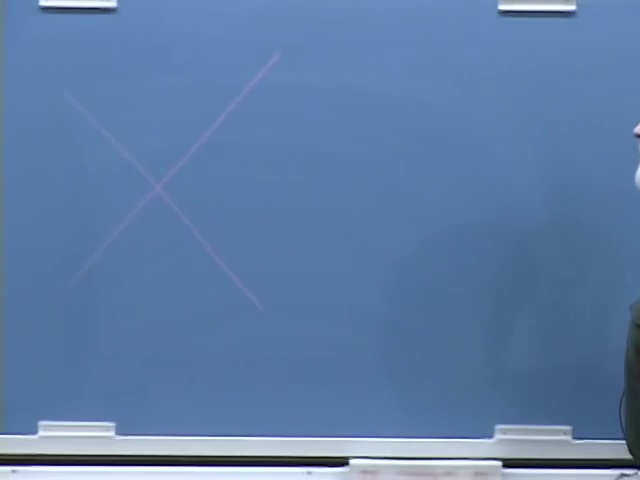
\includegraphics[width=0.68\textwidth]{lecture_09_figure_02.png}
\caption{자연 단위계에서의 호킹 온도 \(T_H=1/(8\pi M)\)}
\lectureframe{00:08:12}
\end{figure}

큰 블랙홀일수록 온도는 낮다. 강의에서는 대표적인 광자를 거슬러 추적해 이를 설명한다. 열복사의 광자는 특성 에너지 \(E_\gamma\sim T_H\)를 가진다. 무한대에 도달했을 때 에너지가 대략 \(M^{-1}\)인 광자는 지평선 가까이에서 출발할 때 훨씬 큰 국소 에너지를 지녔다. 지평선 근처 층에서 무한대까지의 적색편이는 블랙홀이 클수록 더 심해져, 점근 영역에서 측정되는 온도는 더 낮아진다.

\begin{classroomqa}
\audiencequestion{슈바르츠실트 시간이 지평선에서 멈춘다면, 처음에 안으로 떨어져 블랙홀을 만든 광자를 따라가야 할까요?\lecturetimestamp{00:04:19}}
\lecturerresponse{온도 문제를 살피려면 바깥쪽으로 방출된 광자를 따라가면 된다. 광자는 국소적으로 매우 높은 진동수에서 출발해 밖으로 올라오면서 에너지를 잃고 호킹 복사로 도달한다. 처음에 안으로 떨어진 광자의 운명은 별개의 정보 문제다.}
\end{classroomqa}

\section{플랑크 층과 늘어난 지평선}

식~\eqref{eq:l09-local-temperature}의 국소 관계는 어디까지 신뢰할 수 있을까? 강의에서는 반고전적 기술에서 플랑크 길이를 의미를 부여할 수 있는 최단 거리로 본다. 그러면 수학적 지평선에서 바깥쪽으로 대략 플랑크 길이만큼 떨어진 얇은 층에 플랑크 규모의 요동이 차 있는 그림이 떠오른다. 이 층에서는 방출과 흡수가 끊임없이 일어난다.

방출된 양자 가운데 대부분은 탈출하지 못한다. 아주 좁은 바깥쪽 원뿔 방향으로 나아가는 양자만 다시 떨어지지 않는다. 일반적인 각도로 방출된 양자는 지평선으로 되돌아온다. 바깥쪽으로 나가는 들뜸과 안쪽으로 들어오는 들뜸이 충돌해 쌍입자와 다른 입자들을 만들어 낸다. 이런 의미에서 정지 기술에는 극도로 뜨거운 물질로 된 얇은 껍질이 들어 있다.

\begin{figure}[htbp]
\centering
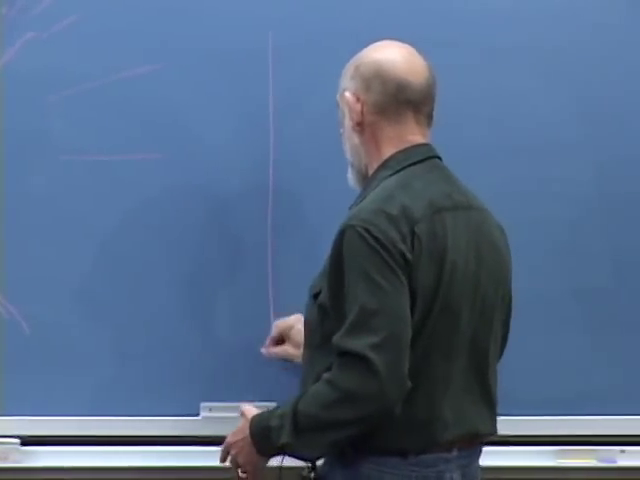
\includegraphics[width=0.74\textwidth]{lecture_09_figure_03.png}
\caption{지평선 근처 복사가 탈출할 수 있는 좁은 원뿔. 국소적으로 방출된 양자의 대부분은 지평선으로 되돌아온다.}
\lectureframe{00:11:38}
\end{figure}

이에 대응하는 시공간 그림도 있다. 지평선에서 멀리 떨어진 곳에서는 가상 요동을 짧은 닫힌 고리로 개략적으로 나타낼 수 있다. 입자와 반입자의 들뜸이 나타났다가 점근 상태가 되기 전에 사라진다는 뜻이다. 지평선 근처에서는 요동이 인과적 경계를 가로지를 수 있다. 외부 관측자에게는 바깥쪽 부분이 지평선에서 방출되었다가 나중에 다시 흡수되는 입자처럼 보인다. 그중 아주 작은 일부가 탈출해 호킹 복사가 된다.

\begin{classroomqa}
\audiencequestion{외부 영역의 그림에서 이런 요동은 \(t=-\infty\)에서 \(t=+\infty\)까지 이어지나요?\lecturetimestamp{00:15:00}}
\lecturerresponse{정확한 고전적 지평선을 사용하면 그런 특이해 보이는 기술이 나온다. 실제로는 지평선에서 플랑크 길이 정도 바깥에 있는 시간꼴 곡면인 늘어난 지평선으로 바꾸어 기술한다. 그러면 방출과 재흡수는 유한한 외부 시간에 일어난다.}
\end{classroomqa}

\begin{figure}[htbp]
\centering
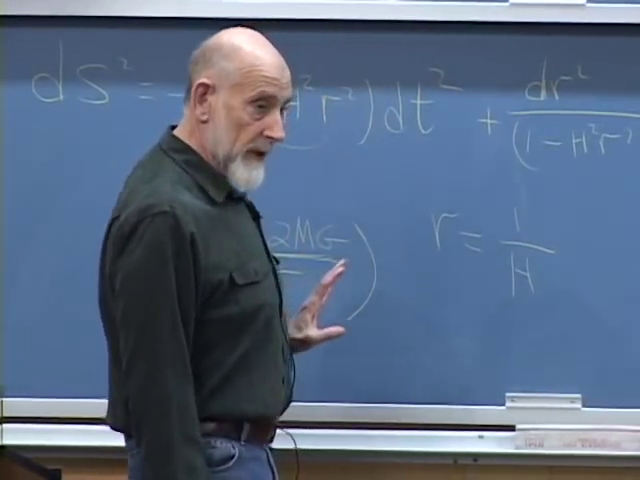
\includegraphics[width=0.72\textwidth]{lecture_09_figure_04.png}
\caption{외부 기술에서 사용하는 고전적 지평선과 그 가까이에 놓인 늘어난 지평선.}
\lectureframe{00:15:52}
\end{figure}

늘어난 지평선은 새로운 불변 경계가 아니다. 반고전적 기하학을 더는 신뢰할 수 없는 위치에 놓은 유효 곡면이다. 물질과 기하학 자체의 양자 요동은 지평선의 정확한 위치를 플랑크 규모로 흐릿하게 만든다. 이 구성에서는 그 불확실성을 하나의 곡면으로 나타내며, 그 위에서는 외부 기술이 유한한 값을 유지한다.

이 국소적 논의만으로는 지평선이 블랙홀에 속하는지 가속하는 우주에 속하는지 알 수 없다. 여기서 드지터 공간으로 넘어간다.

\section{팽창 좌표에서의 드지터 공간}

본 강의는 드지터 시공간의 공간적으로 평탄한 엽절단에서 시작한다.
\begin{equation}
ds^2=-dt^2+e^{2Ht}d\mathbf{x}^2,
\qquad
d\mathbf{x}^2=dx^2+dy^2+dz^2.
\label{eq:l09-flat-slicing}
\end{equation}
상수 \(H\)는 드지터 팽창률이다. 계량은 거리의 제곱을 재므로 인자는 \(e^{2Ht}\)로 나타난다. 좌표 간격이 고정되어 있을 때 물리적 길이는 다음과 같다.
\begin{equation}
D(t)=e^{Ht}\lvert\Delta\mathbf{x}\rvert.
\end{equation}

\begin{figure}[htbp]
\centering
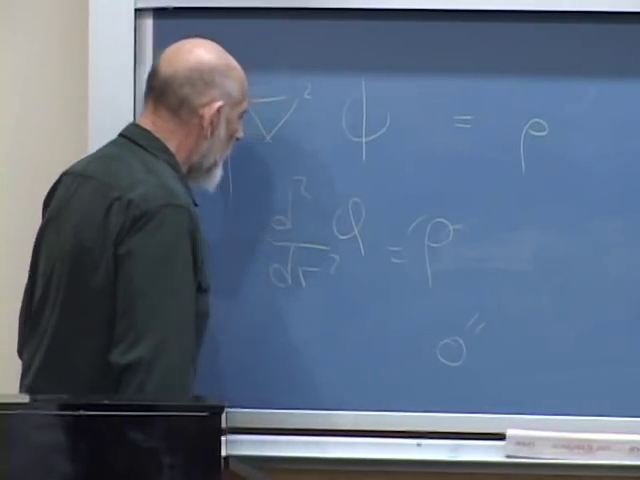
\includegraphics[width=0.78\textwidth]{lecture_09_figure_05.png}
\caption{평탄 좌표로 쓴 지수 팽창 드지터 계량.}
\lectureframe{00:18:50}
\end{figure}

이 좌표에서는 팽창이 명확히 드러나지만, 미래 무한대는 그림 위쪽으로 무한히 멀리 놓인다. 이를 칠판 안으로 가져오려면 등각 시간을 도입한다.
\begin{equation}
\eta=-\frac{1}{H}e^{-Ht},
\qquad
-\infty<\eta<0.
\label{eq:l09-conformal-time}
\end{equation}
그러면
\begin{equation}
dt=\frac{d\eta}{-H\eta},
\qquad
e^{Ht}=-\frac{1}{H\eta},
\end{equation}
이 되고, 식~\eqref{eq:l09-flat-slicing}은 다음과 같이 된다.
\begin{equation}
ds^2=\frac{1}{H^2\eta^2}
\left(-d\eta^2+d\mathbf{x}^2\right).
\label{eq:l09-conformal-metric}
\end{equation}
\(t\to+\infty\)일 때 \(\eta\to0^{-}\)이다. 무한한 고유시간이 유한한 수평선 \(\eta=0\)으로 압축되었다.

\editorialnote{칠판에 적는 동안 시간 변환식을 여러 번 고쳐 쓴다. 일관된 형태는 식~\eqref{eq:l09-conformal-time}이며, 초기 우주 시간은 \(\eta\to-\infty\)에 대응하고 미래 무한대는 \(\eta\to0^{-}\)에 대응한다.}

\begin{figure}[htbp]
\centering
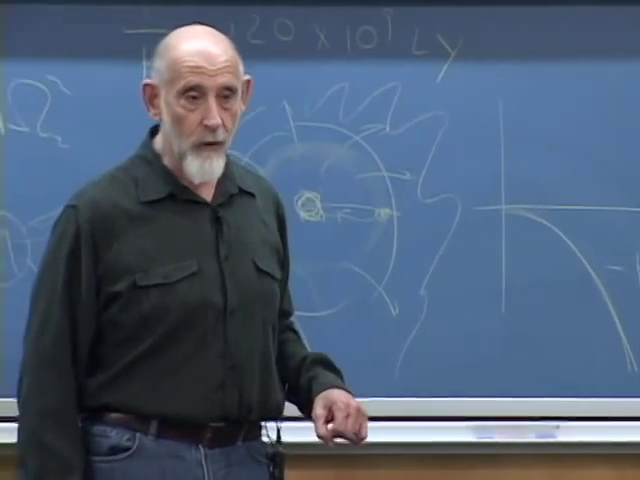
\includegraphics[width=0.82\textwidth]{lecture_09_figure_06.png}
\caption{등각 시간 변환과 등각 평탄 계량.}
\lectureframe{00:21:24}
\end{figure}

등각 인자는 시간 성분과 공간 성분 모두에 곱해지므로 영방향은 바뀌지 않는다. 방사형 광선에 대해서는
\begin{equation}
ds^2=0
\quad\Longrightarrow\quad
-d\eta^2+dx^2=0
\quad\Longrightarrow\quad
\frac{dx}{d\eta}=\pm1.
\label{eq:l09-null-rays}
\end{equation}
따라서 등각 도표에서 빛은 \(45^\circ\) 방향으로 이동한다. 좌표 변환이 유용한 이유가 여기에 있다. 인과적으로 도달할 수 있는 영역을 눈으로 확인할 수 있다.

\section{한 관측자의 인과 패치}

고유시간이 무한히 이어지는 관측자를 생각해 보자. 압축 도표에서 관측자의 세계선은 \(\eta=0\) 위의 한 점에서 끝난다. 관측자가 받을 수 있는 모든 신호는 그 끝점의 과거 광원뿔 안에 놓인다. 광원뿔 바깥의 사건은 관측자가 아무리 오래 기다려도 관측자와 정보를 주고받을 수 없다.

\begin{figure}[htbp]
\centering
\includegraphics[width=0.78\textwidth]{lecture_09_figure_07.png}
\caption{등각 드지터 좌표에서 관측자의 극한 과거 광원뿔.}
\lectureframe{00:24:38}
\end{figure}

다른 관측자에게는 다른 광원뿔이 있다. 두 관측자가 접근할 수 있는 영역은 겹치지만, 어느 쪽도 시공간 전체가 아니다. 이제부터는 첫 번째 관측자의 관점을 택하고, 그 과거 광원뿔을 관측자의 인과 패치라고 부르겠다.

그림만 보면 패치가 미래로 갈수록 줄어드는 듯하지만, 좌표상 폭은 고유거리가 아니다. 일정한 \(\eta\) 단면에서 관측자 \(x=0\)와 지평선 \(x=\Delta x\) 사이의 물리적 거리 제곱은 다음과 같다.
\begin{equation}
D^2=\frac{(\Delta x)^2}{H^2\eta^2}.
\label{eq:l09-horizon-distance-start}
\end{equation}
지평선은 \(45^\circ\) 영선이며 \(\eta=0\)에서 끝나므로
\begin{equation}
\Delta x=\lvert\eta\rvert.
\end{equation}
이를 대입하면
\begin{equation}
D_{\rm hor}^2=\frac{1}{H^2},
\qquad
D_{\rm hor}=\frac{1}{H}.
\label{eq:l09-horizon-radius}
\end{equation}
좌표상 간격은 줄어들지만 등각 인자는 그 감소를 정확히 상쇄할 만큼 커진다. 고유 지평선 반지름은 일정하다.

\begin{figure}[htbp]
\centering
\includegraphics[width=0.80\textwidth]{lecture_09_figure_08.png}
\caption{줄어드는 좌표 간격을 고정된 고유거리 \(H^{-1}\)로 바꾸는 칠판 유도.}
\lectureframe{00:28:42}
\end{figure}

\section{정적 패치}

고정된 지평선 반지름을 보면 중심 관측자에 맞춘 좌표를 도입할 수 있다. 좌표 변환을 유도하지 않고 강의에서는 결과를 바로 쓴다.
\begin{equation}
ds^2=
-\left(1-H^2r^2\right)d\tau^2
+\frac{dr^2}{1-H^2r^2}
+r^2d\Omega_2^2.
\label{eq:l09-static-patch}
\end{equation}
계수는 \(r\)에 의존하며 \(\tau\)에는 의존하지 않는다. 이 좌표계는 다음 범위의 관측자 정적 패치를 덮는다.
\begin{equation}
0\le r<\frac{1}{H}.
\end{equation}

\begin{figure}[htbp]
\centering
\includegraphics[width=0.88\textwidth]{lecture_09_figure_09.png}
\caption{드지터 정적 패치 계량과 슈바르츠실트 인자와의 비교.}
\lectureframe{00:34:22}
\end{figure}

슈바르츠실트 계량과의 유사성은 바로 드러난다.
\begin{equation}
f_{\rm dS}(r)=1-H^2r^2,
\qquad
f_{\rm Schw}(r)=1-\frac{2G_NM}{r}.
\end{equation}
두 경우 모두 정적 좌표에서 지평선은 \(f(r)=0\)인 곳에 생긴다. 드지터 공간에서는
\begin{equation}
1-H^2r^2=0
\quad\Longrightarrow\quad
r_H=H^{-1}.
\end{equation}
그곳에서 좌표계가 특이해지는데, 슈바르츠실트 좌표가 블랙홀 지평선에서 특이해지는 것과 같다. 그러나 전역적인 기하학은 중요한 점에서 다르다. 블랙홀 관측자는 바깥에 서서 안을 바라보지만, 드지터 관측자는 안에 서서 바깥을 바라본다.

\begin{classroomqa}
\audiencequestion{자유롭게 놓아둔 입자들이 지수적으로 팽창하는 우주에서 서로 멀어지는데, 기하학은 어떻게 정적일 수 있나요?\lecturetimestamp{00:36:06}}
\lecturerresponse{정적이라는 말은 모든 입자가 고정된 채 있다는 뜻이 아니다. 계량 계수와 반복 실험의 결과가 시작 시각에 의존하지 않는다는 뜻이다. 입자 두 개를 지금 놓아두면 서로 가속하며 멀어지고, 나중에 같은 실험을 반복해도 똑같은 운동이 일어난다.}
\end{classroomqa}

\begin{classroomqa}
\audiencequestion{서로 멀어지는 두 입자는 상대방의 빛이 적색편이되는 것을 보나요?\lecturetimestamp{00:38:34}}
\lecturerresponse{그렇다. 두 입자 사이의 거리가 늘어나므로 상대적 적색편이가 생긴다. 관측자에 맞춘 계량이 시간에 무관하더라도 그렇다.}
\end{classroomqa}

\section{내부에서 관측되는 온도}

슈바르츠실트 공간과 드지터 공간의 지평선 근처 구조는 국소적으로 동등하다. 따라서 드지터 지평선도 열적 양자를 방출하고 다시 흡수한다. 드물게 방출된 광자는 중심 관측자 쪽으로 안쪽을 향해 이동하면서 정적 패치의 중력 퍼텐셜을 거슬러 올라갈 때 에너지를 잃는다. 중심에서 측정되는 긴스버그--호킹 온도는 자연 단위계에서 다음과 같다.
\begin{equation}
T_{\rm dS}=\frac{H}{2\pi}
\label{eq:l09-de-sitter-temperature}
\end{equation}
반지름 \(r\)에 정지한 온도계는 톨먼 적색편이를 반영한 다음 온도를 읽는다.
\begin{equation}
T_{\rm local}(r)=
\frac{T_{\rm dS}}{\sqrt{1-H^2r^2}},
\label{eq:l09-tolman}
\end{equation}
이는 \(r\to H^{-1}\)일 때 발산하며, 지평선 근처에서는 식~\eqref{eq:l09-local-temperature}으로 돌아간다.

\editorialnote{강의에서는 식~\eqref{eq:l09-de-sitter-temperature}과 \eqref{eq:l09-tolman}을 명시적으로 쓰지 않고 지평선 거리와 적색편이로부터 온도 규모를 구한다. 이 식들은 그 논증의 표준적인 정규화를 나타낸다.}

현재 관측되는 후기 우주의 가속을 설명하기 위해 강의에서는 다음 주기 추정값을 사용한다.
\begin{equation}
H^{-1}\sim 20\times10^9\ {\rm light\ years}.
\label{eq:l09-lecture-horizon-estimate}
\end{equation}
그러면 전형적인 지평선 광자의 파장은 수십억 광년과 비슷한 규모가 된다. 이는 우주 마이크로파 배경 복사가 아니라, 그보다 훨씬 더 차가운 복사다.

조작적 사고실험은 우주론적 규모의 낚싯대와 같다. 앨리스는 \(r=0\)에 머물면서 데이터를 전송할 수 있는 매우 긴 줄에 온도계를 달고, 우주의 척력이 기기를 바깥으로 끌고 가게 둔다. 지평선 바로 앞에서 기기를 멈춘 뒤 신호가 돌아오기를 기다려 국소 온도가 높다는 것을 확인한다. 중심에 놓인 앨리스 곁의 온도계는 작은 값 \(H/(2\pi)\)을 가리킨다. 서로 다른 중력 퍼텐셜에서 측정했기 때문에 하나의 지평선에서 두 값이 모두 나타난다.

\section{지평선 통과}

고전적인 외부 관측 기술은 익숙한 블랙홀 이야기와 비슷하다. 중심에 있는 밥은 앨리스가 멀어지는 모습을 지켜본다. 앨리스의 신호는 점점 더 적색편이되고 도달 간격도 점점 길어진다. 앨리스는 지평선에 납작하게 달라붙은 듯 보이다가 결국 희미해진다. 나중에 여행을 떠난 제인은 경계 근처에 퇴적층처럼 쌓이는 또 하나의 더 얇은 층으로 보인다.

\begin{classroomqa}
\audiencequestion{우리의 관점에서 보면 물체는 우주 지평선을 실제로 통과하나요?\lecturetimestamp{00:45:30}}
\lecturerresponse{정적 관측자의 고전적 기술에서는 그렇지 않다. 물체의 겉보기 위치가 지평선에 다가가는 동안 신호는 적색편이되고 희미해진다. 그러나 물체와 함께 자유 낙하하는 관측자의 기술에서는 국소적으로 특이한 표면을 만나지 않고 지평선을 통과한다.}
\end{classroomqa}

\begin{classroomqa}
\audiencequestion{지평선은 통과하지 않은 채 가까이에 머무는 관측자에게만 뜨거운 건가요? 낙하 관측자는 지평선을 통과한다고 해서 타지는 않는 거죠?\lecturetimestamp{00:48:27}}
\lecturerresponse{앨리스는 자신의 기준계에서 지평선을 매끄럽게 통과한다. 극단적인 온도는 정지 관측자의 기술에서 나타난다. 밥이 지평선에 가까워지는 앨리스를 점점 더 자세히 관측하려면 점점 더 짧은 파장의 빛을 비춰야 한다. 하이젠베르크 현미경을 이용해 그렇게 관측하려 하면, 관측 대상이 탈 만큼의 에너지가 전달된다.}
\end{classroomqa}

이는 두 국소 사건 사이의 모순이 아니다. 정지 관측자와 낙하 관측자는 근본적으로 다른 측정을 한다. 지평선 상보성은 한 관측자가 중복된 정보를 직접 대조할 수 없으면서도 두 기술이 모두 타당할 수 있는 방법을 묻는다.

\section{진공 척력을 설명하는 뉴턴 모형}

이때 한 학생이 블랙홀의 중력 우물에 해당하는 것이 무엇인지 묻는다. 서스킨드는 뉴턴 모형을 구성해 답한다. 중력 퍼텐셜을 \(\phi\)라 하면 시험 입자의 가속도는 다음과 같다.
\begin{equation}
\mathbf{a}=-\boldsymbol{\nabla}\phi.
\end{equation}
보통의 비상대론적 물질에 대해서는 푸아송 방정식이 다음과 같다.
\begin{equation}
\nabla^2\phi=4\pi G_N\rho.
\label{eq:l09-poisson}
\end{equation}

\begin{classroomqa}
\audiencequestion{블랙홀 효과가 중력 우물에서 생긴다면, 드지터 공간에서는 무엇이 이에 대응하는 원천인가요?\lecturetimestamp{00:49:36}}
\lecturerresponse{진공 에너지 자체가 공간적으로 균일한 중력 원천을 제공한다. 뉴턴 기술에서는 이것이 \(1/r\) 우물이 아니라 이차 퍼텐셜을 만든다.}
\end{classroomqa}

\begin{figure}[htbp]
\centering
\includegraphics[width=0.78\textwidth]{lecture_09_figure_10.png}
\caption{푸아송 방정식과 강의에서 개략적으로 쓴 방사형 이계도함수 형태.}
\lectureframe{00:51:38}
\end{figure}

칠판의 유도에서는 정규화와 구면 좌표의 측도 항, 압력을 생략하고 처음에는 전체 부호까지도 생략해 문제를 다음과 같이 단순화한다.
\begin{equation}
\frac{d^2\phi}{dr^2}\sim H^2.
\end{equation}
핵심적인 추론은 원천이 일정하면 이차함수가 된다는 것이다. 드지터 척력에 맞는 부호를 택하면
\begin{equation}
\phi_{\rm dS}(r)=-\frac{1}{2}H^2r^2,
\qquad
a_r=-\frac{d\phi_{\rm dS}}{dr}=H^2r.
\label{eq:l09-de-sitter-potential}
\end{equation}
가속도는 바깥쪽을 향하며 거리에 비례해 커진다. \(\ddot r=H^2r\)을 풀면
\begin{equation}
r(\tau)=A e^{H\tau}+B e^{-H\tau},
\end{equation}
을 얻으므로, 증가하는 해가 지수적 분리를 재현한다.

\begin{figure}[htbp]
\centering
\includegraphics[width=0.76\textwidth]{lecture_09_figure_11.png}
\caption{균일한 원천을 나타내는 방정식과 드지터 이차 퍼텐셜.}
\lectureframe{00:53:32}
\end{figure}

\editorialnote{일반 상대론에서 균일한 유체의 약한 장 근사 가속도는 \(\rho+3p\)에 의존하며 \(\rho\)에만 의존하지 않는다. 진공 에너지는 \(p=-\rho\)이므로 \(\rho+3p=-2\rho\)이고, 이에 따라 가속도는 척력으로 작용한다. 식~\eqref{eq:l09-de-sitter-potential}은 정규화를 올바르게 적용한 드지터 결과다. 칠판의 계산에서는 이차 의존성과 부호만 살펴본다.}

중심에 보통의 질량 \(M\)를 놓아 보자. 그러면 퍼텐셜은 정성적으로 다음과 같이 된다.
\begin{equation}
\phi(r)=-\frac{G_NM}{r}-\frac{1}{2}H^2r^2,
\label{eq:l09-combined-potential}
\end{equation}
방사 방향 가속도는
\begin{equation}
a_r=-\frac{G_NM}{r^2}+H^2r.
\end{equation}
이다. 작은 \(r\)에서는 국소적인 인력이 우세하고, 큰 \(r\)에서는 진공 척력이 우세하다. 두 효과가 균형을 이루는 위치는 다음과 같다.
\begin{equation}
r_\ast=\left(\frac{G_NM}{H^2}\right)^{1/3}.
\label{eq:l09-turnaround}
\end{equation}
이것이 강의에서 그린 퍼텐셜 최대점을 더 명확히 나타낸 결과다. 가까운 중력 결합계는 서로 붙어 있을 수 있지만 충분히 멀리 떨어진 은하들은 가속하며 멀어지는 이유를 정성적으로 설명해 준다.

\begin{figure}[htbp]
\centering
\includegraphics[width=0.78\textwidth]{lecture_09_figure_12.png}
\caption{보통의 \(1/r\) 인력과 위가 아래로 향한 포물선 모양의 드지터 퍼텐셜을 합친 결과.}
\lectureframe{00:58:20}
\end{figure}

\begin{classroomqa}
\audiencequestion{보통의 힘도 여전히 중요한가요, 아니면 진공 척력이 결국 모든 물질의 섬을 찢어 놓나요?\lecturetimestamp{00:57:29}}
\lecturerresponse{모든 힘을 고려해야 한다. 충분히 작은 규모에서는 전자기적 결합과 국소 중력이 우세하다. 진공 척력은 \(H^{-1}\)과 결합 질량에 맞는 균형 규모로 정해지는 엄청나게 큰 거리에 걸쳐서만 중요해진다.}
\end{classroomqa}

\section{하나의 원천, 여러 이름}

이제 논의는 용어를 짚어 보며 잠시 멈춘다. 여기서 사용하는 모형에서 진공 에너지, 우주 상수, 암흑 에너지는 서로 더해지는 세 가지 물질이 아니다. 이들은 같은 \(w=-1\) 원천을 세 가지 방식으로 기술한 것이다. 아인슈타인 방정식의 상수항, 진공의 로런츠 불변 에너지 밀도, 후기 우주 가속을 일으키는 성분이라고 부를 수 있다.

\begin{classroomqa}
\audiencequestion{균일한 뉴턴 원천과 양자 진공 에너지가 별개의 효과로 함께 존재하나요?\lecturetimestamp{00:59:14}}
\lecturerresponse{아니다. 균일한 밀도는 같은 원천을 뉴턴 모형으로 나타낸 것이다. 진공 에너지, 우주 상수, 그리고 이 강의에서 말하는 암흑 에너지는 하나의 물리적 성분을 가리킨다.}
\end{classroomqa}

\begin{classroomqa}
\audiencequestion{그렇다면 같은 현상을 고전적으로도, 양자역학적으로도 기술할 수 있나요?\lecturetimestamp{01:00:32}}
\lecturerresponse{전자 질량의 일부가 양자적 기원을 갖듯이, 그 미시적 기원은 양자역학적일 수 있다. 유효 에너지 밀도를 알게 되면 그것은 고전 중력 방정식에 보통의 원천으로 들어간다. 관측된 값의 궁극적인 기원은 아직 모른다.}
\end{classroomqa}

플랑크 단위계에서 관측된 진공 에너지 밀도는 엄청나게 작다.
\begin{equation}
\rho_\Lambda\sim10^{-123}\rho_{\rm Pl},
\label{eq:l09-planck-smallness}
\end{equation}
정확한 값은 플랑크 밀도에 사용하는 관례에 따라 달라진다. 이 작은 값이 우주 상수 문제다. 지평선이 그토록 큰 이유도 여기에 있다. 4차원에서는
\begin{equation}
H^2=\frac{8\pi G_N}{3}\rho_\Lambda,
\qquad
r_H=H^{-1}.
\end{equation}
\(H\)가 더 크다면 지평선은 더 작아지고 중심의 드지터 온도는 더 높아지며, 척력 가속도 \(H^2r\)도 더 강해질 것이다.

\begin{classroomqa}
\audiencequestion{작은 우주 상수는 플랑크 상수 및 양자 요동과 관련이 있나요?\lecturetimestamp{01:03:27}}
\lecturerresponse{깔끔하게 비교하려면 무차원 플랑크 단위계를 사용하면 된다. 이 단위계에서는 \(G_N=\hbar=c=1\)이다. 그 단위계에서 진공 밀도는 자연스러운 플랑크 밀도보다 약 \(123\) 자릿수만큼 작다. 이 계층을 설명하는 것은 기초 물리학의 핵심 난제 가운데 하나다.}
\end{classroomqa}

\begin{classroomqa}
\audiencequestion{진공 에너지는 반드시 정확히 일정한 우주 상수여야 하나요? 가속을 일으키는 성분이 줄어들다가 결국 0에 이를 수도 있나요?\lecturetimestamp{01:04:52}}
\lecturerresponse{논리적으로 가능한 대안이다. 동역학적 암흑 에너지 장은 시간에 따라 변할 수 있다. 강의에서 상수인 경우를 택한 것은 당시 이용 가능했던 관측이 우주 상수에 가까운 거동을 점점 더 지지했기 때문이지, 모든 대안이 불가능하다고 입증되었기 때문은 아니다.}
\end{classroomqa}

\section{먼 미래의 천문학}

점근적으로 드지터인 우주에서는 중력적으로 묶여 있지 않은 구조들이 결국 관측자의 지평선을 넘어간다. 우주 마이크로파 배경 복사는 검출할 수 없는 수준으로 적색편이된다. 먼 은하들은 시야에서 사라진다. 살아남은 천문학자는 어둠에 잠긴 패치 안에서 하나로 합쳐진 국소 중력 섬만 보게 될 수도 있다.

\begin{classroomqa}
\audiencequestion{망원경이 없다면 먼 은하들이 사라진 사실조차 알아차릴 수 있을까요?\lecturetimestamp{01:06:17}}
\lecturerresponse{아마 알아차리지 못할 것이다. 더 근본적인 문제는 이렇다. 미래 관측자들은 정교한 장비를 갖추더라도 오늘날 우리가 팽창을 추론하는 데 쓰는 먼 천체와 우주 마이크로파 배경을 잃어버릴 수 있다.}
\end{classroomqa}

그렇다면 오래된 섬 우주 모형이 설득력 있어 보일 수 있다. 올베르스의 역설도 다른 결론을 강요하지 않을 것이다. 올베르스의 역설은 광원을 내는 천체들이 무한하고 정적이며 균일하게 분포한다고 가정하지만, 미래 관측자가 보게 되는 것은 국소적인 섬 안에 있는 유한한 수의 별뿐이기 때문이다. 암흑 에너지가 빈 공간에서 대체 은하를 계속 만들어 내는 것은 아니다.

정확한 드지터 공간에서 지평선은 국소 은하를 중심으로 줄어들지 않는다. 물리적 반지름 \(H^{-1}\)은 은하보다 훨씬 크며 일정하게 유지된다. 사라지는 것은 고정된 인과적 경계 너머로 실려 가는 비결합 물질이다.

\begin{classroomqa}
\audiencequestion{은하에서 튕겨 나간 별들을 큰 규모의 기하학을 검출하기 위한 시험체로 쓸 수 있을까요?\lecturetimestamp{01:11:25}}
\lecturerresponse{한동안은 가능하다. 방출된 천체와 긴 기준선에 걸친 빛 신호로 기하학을 탐사할 수 있다. 하지만 효과가 뚜렷해지는 것은 십억 광년의 상당 부분에 해당하는 거리 규모에서뿐이므로, 실험에는 우주론적 시간이 걸릴 것이다.}
\end{classroomqa}

\begin{classroomqa}
\audiencequestion{먼 지평선이 이미 우주의 대부분을 우리에게서 가리고 있지는 않다는 것을 어떻게 알 수 있나요?\lecturetimestamp{01:11:45}}
\lecturerresponse{우리는 팽창을 측정하고 대규모 기하학을 재구성할 만큼 충분한 은하, 적색편이, 배경 복사를 이미 관측하고 있다. 그런 추적 수단을 잃게 될 미래 관측자에게는 추론이 훨씬 더 어려울 것이다.}
\end{classroomqa}

\begin{classroomqa}
\audiencequestion{지평선이 안드로메다 바로 너머에 있다면 그 존재가 분명히 드러날까요?\lecturetimestamp{01:12:19}}
\lecturerresponse{그렇다. 그렇게 작은 지평선이려면 \(H\)가 훨씬 더 커야 하고, 그에 따른 척력이 안드로메다의 운동을 크게 바꿀 것이다. 실제로 측정된 값에 따르면 점근적 지평선의 규모는 그보다 훨씬 크다.}
\end{classroomqa}

\begin{classroomqa}
\audiencequestion{우리 지평선 너머에서 새로운 빅뱅이 일어나고 있을 수도 있나요?\lecturetimestamp{01:13:25}}
\lecturerresponse{지평선 너머의 사건은 우리에게도 후손에게도 보이지 않는다. 이와 관련되면서 더 정확하게 말할 수 있는 가능성인 영원한 급팽창에서의 거품 핵생성은 강의 뒷부분에서 소개한다.}
\end{classroomqa}

로켓과 시계, 그리고 수십억 년의 시간이 있다면 미래 관측자들은 패치의 상당 부분을 가로질러 탐사선을 보내고 계량을 재구성할 수 있다. 그러나 보통의 실험실 시간이나 문명이 존속하는 시간 규모에서는 그 효과에 접근하기가 거의 불가능하다. 이 구분을 통해 팽창을 발견할 수 없다는 지나치게 강한 주장을 바로잡을 수 있다. 원리적으로 금지된 것이 아니라, 실제로 확인하기까지 우주론적 규모의 시간이 걸리는 것이다.

\begin{classroomqa}
\audiencequestion{미래의 탐사자들이 열적 재귀를 기다리는 것보다 훨씬 일찍 기하학을 알아낼 수 있나요?\lecturetimestamp{01:21:40}}
\lecturerresponse{물론이다. 재귀를 측정 방법으로 제안하는 것이 아니다. 십억 광년 규모의 기준선에 걸쳐 빛 신호를 주고받는 탐사자들은 훨씬 짧은 시간 안에 정적 패치를 지도화할 수 있다. 물론 그 시간도 우주론적 규모이기는 하다.}
\end{classroomqa}

\begin{classroomqa}
\audiencequestion{그런 탐사자들이 보내오는 정보가 적색편이 때문에 모두 사라질까?\lecturetimestamp{01:23:24}}
\lecturerresponse{그들이 지평선 안쪽의 충분히 작은 규모를 탐사한다면 그렇지 않다. 십억 광년 정도의 기준선만으로도 팽창에 민감해지면서 적색편이는 중간 정도에 그친다. 이 실험은 주로 엄청나게 긴 시간 때문에 제약을 받는다.}
\end{classroomqa}

\section{유한한 엔트로피와 재귀}

정적 패치는 열역학적 의미에서 비어 있지 않습니다. 그 지평선의 면적은
\begin{equation}
A_H=4\pi H^{-2},
\end{equation}
온도는 \(T_{\rm dS}=H/(2\pi)\)이며, 엔트로피는
\begin{equation}
S_{\rm dS}=\frac{A_H}{4G_N}
=\frac{\pi}{G_NH^2}
\label{eq:l09-de-sitter-entropy}
\end{equation}
단위계 \(\hbar=c=k_B=1\)에서 주어집니다. 엔트로피는 유한합니다. 따라서 적절한 주의를 기울인다면, 정적 패치를 정상적인 기술에서 들뜸이 지평선 부근에 집중된 유한 엔트로피 열적 공동으로 그려 볼 수 있습니다.

평형 상태의 보통 기체 상자는 짧은 시간 척도에서는 아무런 특징도 없어 보이지만, 통계역학은 요동을 금지하지 않습니다. 어떤 거시 상태의 엔트로피가 평형 상태보다 \(\Delta S\)만큼 낮다면, 그 상태의 확률은 대략
\begin{equation}
P\sim e^{-\Delta S}.
\label{eq:l09-fluctuation-probability}
\end{equation}
기다리는 시간은 이에 따라
\begin{equation}
t\sim t_0 e^{\Delta S}.
\end{equation}
만큼 늘어납니다. 유한한 계가 이전 상태와 임의로 가까운 상태를 다시 방문하기까지 걸리는 시간은 푸앵카레 재귀 시간이며,
\begin{equation}
t_{\rm rec}\sim H^{-1}e^{S_{\rm dS}}.
\label{eq:l09-recurrence}
\end{equation}
우리 지평선의 \(S_{\rm dS}\)가 대략 \(10^{120}\) 규모이므로, 강의에서는 그 척도를 \(e^{10^{120}}\)로 요약합니다. 앞의 계수가 연 단위인지, 허블 시간 단위인지, 미시적 단위인지는 이중 지수에 비하면 중요하지 않습니다.

\begin{figure}[htbp]
\centering
\includegraphics[width=0.76\textwidth]{lecture_09_figure_13.png}
\caption{칠판에 엄청난 지수적 대기 시간이 적힌 재귀 논의.}
\lectureframe{01:16:24}
\end{figure}

그러한 재귀가 일어나기 전에도 더 작은 요동은 훨씬 흔합니다. 방 안의 분자들이 모두 한쪽 구석에 모일 수도 있고, 복잡한 소용돌이가 잠시 생길 수도 있습니다. 강의에서 장난스럽게 나열한 예로는 열운동이 코끼리를 조립할 수도 있습니다. 필요한 엔트로피 감소가 작을수록 요동에 드는 비용도 낮습니다.

\begin{classroomqa}
\audiencequestion{푸앵카레 재귀는 양자역학의 고유한 결과인가요?\lecturetimestamp{01:25:44}}
\lecturerresponse{아닙니다. 재귀와 희귀한 요동은 고전 통계역학에서도 이미 나타납니다. 이를 드시터 공간에 적용하는 것은 언젠가 수정될 수도 있는 현재의 물리적 틀에 기반하지만, 열역학과 통계적 추론은 우리가 아는 가장 견고한 체계에 속합니다.}
\end{classroomqa}

확률 자체의 의미는 미래 이론에서 더 깊어질 수도 있습니다. 서스킨드는 그렇지 않다고 주장하지 않습니다. 그가 말하는 더 제한적인 요점은, 장시간에 걸친 함의가 낯설다는 이유만으로 통계역학을 버리면 물리학에서 가장 잘 검증된 구성 원리 중 하나를 포기하게 된다는 것입니다.

\section{볼츠만 두뇌와 전형적인 관측자}

열적 요동이 빅뱅과 비슷한 상태 전체를 만들어 낸다고 가정해 봅시다. 그러려면 엔트로피가 엄청나게 감소해야 합니다. 태양계 하나를 만들어 내는 요동은 비용이 더 적고, 이미 따뜻한 지구를 만들어 내는 요동은 그보다도 비용이 적습니다. 필요한 것이 관측자 하나뿐이라면, 가장 비용이 적은 요동은 겉보기 기억을 온전히 갖춘 기능하는 뇌만 만들어 낼 수도 있습니다. 이런 가상의 관측자를 볼츠만 두뇌라고 부릅니다.

쟁점은 기이한 요동 하나가 논리적으로 가능한지 여부가 아닙니다. 우주론 모형이 거의 모든 관측자를 그런 요동으로 만들어진 관측자라고 예측하는지가 문제입니다. 우리는 자신이 터무니없이 비전형적인 경우가 아니라고 가정하고 관측 결과를 추론합니다. 일관된 우주 역사를 지닌 보통의 관측자보다 고립된 열적 두뇌가 지수적으로 더 많다고 보는 이론은 그런 추론의 근거를 흔듭니다.

따라서 볼츠만 두뇌 문제는 정량적인 일관성 검사를 가리킵니다. 보통의 관측자가 얼마나 있을지와 요동으로 생겨난 관측자가 얼마나 있을지를 비교합니다. 후자가 우세하다면 진공이 그들이 증식하기 전에 붕괴해야 하거나, 측도를 바꾸거나, 우주론의 가정을 재검토해야 합니다.

자외선--적외선 연결에 관한 앞선 질문은 여기서 명시적으로 미뤄 둡니다. 재귀 논증은 그 별개의 문제를 해결하지 않아도 성립합니다.

\section{영원한 인플레이션과 거품 우주}

다음으로 강의는 완전한 유도를 시도하지 않은 채 두 번째 확률 문제를 소개합니다. 준안정 드시터 진공에서는 진공 에너지가 더 낮은 거품이 핵생성될 수 있습니다. 거품 벽은 팽창하고, 내부는 열린 프리드먼--로버트슨--워커 우주로 진화할 수 있습니다. 한편 주위의 인플레이션 영역은 계속 팽창하면서 거품을 더 만들어 냅니다.

\begin{figure}[htbp]
\centering
\includegraphics[width=0.74\textwidth]{lecture_09_figure_14.png}
\caption{인플레이션하는 드시터 배경 안에 그려진, 진공 에너지가 더 낮은 거품.}
\lectureframe{01:29:38}
\end{figure}

핵심은 개체 수가 지수적으로 늘어난다는 점입니다. 새로운 물리적 부피가 거품이 제거하는 부피보다 더 빠르게 생겨나므로, 거품 영역의 수는 한없이 증가합니다. 거품마다 서로 다른 낮은 에너지 상태에 자리 잡을 수 있으므로, 유효한 물리 법칙도 서로 다를 수 있습니다.

통계적 어려움을 드러내기 위해, Susskind는 먼저 우주론을 떠나 자원은 유한하지만 그 양은 알려지지 않은 상황에서 인구가 지수적으로 증가하는 경우를 생각한다. 살았거나 앞으로 살아갈 모든 사람 가운데 관측자가 전형적이라고 가정하자. 인구가 세대마다 두 배로 늘다가 어느 시점에 끝난다면, 전체 인구의 절반은 마지막 세대에 살고, 사분의 삼은 마지막 두 세대에, 팔분의 칠은 마지막 세 세대에 산다.
\begin{equation}
f_n=1-2^{-n}.
\label{eq:l09-last-generations}
\end{equation}
그렇다면 전형성에 따르면 우리는 불편할 만큼 종말에 가까운 시기에 살고 있는 셈이다. 총 자원 공급량에 대해 아무것도 모른다 해도 그렇다. 이는 인류 멸종을 신뢰할 만하게 예측하려는 주장이 아니다. 지수적 성장이 집계 결과를 절단값에 좌우되게 만든다는 경고다.

동전 던지기 예시는 보통의 전형성 가정을 더 명료하게 보여 줍니다. 많은 실험자가 각각 공정한 동전을 \(N\)번 던진다면, 압도적 다수는
\begin{equation}
n_H=\frac{N}{2}+O(\sqrt{N}).
\end{equation}
을 얻습니다. 극단적으로 드문 결과를 얻은 관측자라면, 근거도 없이 자신이 터무니없이 희귀한 꼬리 부분에 있다고 가정하기보다 먼저 모형이나 동전에 문제가 있는지 의심해야 합니다. 우주론에서 확률을 다룰 때도 같은 전형성 직관을 사용하지만, 모집단이 무한하다면 잘 정의된 계수 방법이 필요합니다.

\section{에셔의 경계와 측도 문제}

서스킨드가 든 기하학적 비유는 M.\ C.\ 에셔의 \emph{원형 극한 IV}입니다. 원반을 천사와 악마가 채우고 있으며, 경계에 가까워질수록 도형이 작아 보입니다. 이 그림이 나타내는 쌍곡기하학에서는 도형들이 서로 동등하며, 유클리드적으로 보이는 크기만 투영 때문에 달라집니다.

\begin{figure}[htbp]
\centering
\includegraphics[width=0.76\textwidth]{lecture_09_figure_15.png}
\caption{원형 경계 가까이에서 지수적으로 증식하는 도형을 대신해 칠판에 그린 그림.}
\lectureframe{01:37:54}
\end{figure}

에셔에게 주어진 시간과 잉크, 인내심이 유한하다고 상상해 봅시다. 그는 가장자리 가까이에서 결국 그리기를 멈추고, 몇몇 도형은 미완성으로 남겨 둘 수도 있습니다. 쌍곡 반지름에 따라 도형 수가 지수적으로 늘어나므로, 유한한 바깥층에는 그려진 도형 전체 가운데 일정한 비율이 들어갑니다. 경계가 아무리 바깥으로 옮겨져도 마지막 층에 대략 절반이 놓일 수 있습니다.

이제 천사와 악마의 비율을 물어봅시다. 이상적인 무한 패턴에서는 대칭성 때문에 수가 같으리라고 볼 수 있습니다. 그러나 유한한 계수에서는 경계를 조금 다르게 잡는 것만으로도 한쪽 유형의 도형이 훨씬 더 많이 포함될 수 있습니다. 계수 대부분이 경계 가까이에 몰려 있으므로, 경계를 조금만 변형해도 답이 상당한 정도로 달라집니다.

\begin{figure}[htbp]
\centering
\includegraphics[width=0.76\textwidth]{lecture_09_figure_16.png}
\caption{지수적으로 증가하는 패턴에서는 경계가 계수를 좌우한다.}
\lectureframe{01:43:06}
\end{figure}

영원한 인플레이션에서도 같은 모호성이 나타납니다. 어떤 시간 절단면 아래에 있는 파란색과 분홍색 거품 우주를 센 뒤 절단면을 더 늦은 시점으로 옮겨 봅시다. 두 수 모두 발산하며, 그 비율은 \emph{시간}을 어떻게 정의하고 절단면을 어떻게 그리는지에 민감하게 달라질 수 있습니다. 확률 측도란 무한한 모집단을 조절해 상대적 확률을 추출하는 규정입니다. 서로 그럴듯한 규정들이 같은 결과에 이르지 못하는 문제가 측도 문제입니다.

\begin{classroomqa}
\audiencequestion{이 절단 문제는 재규격화와 관련이 있나요?\lecturetimestamp{01:45:43}}
\lecturerresponse{비유적인 연관성은 있습니다. 양자장론에서는 격자나 자외선 절단을 도입하고, 이를 세분화하면서 조절자의 경계 세부 사항에 좌우되지 않는 양을 찾습니다. 우주론자들도 영원한 인플레이션에서 그만큼 견고한 결과를 추출하기를 바라지만, 여기서 논의하는 틀에는 아직 그에 필적할 만한 결정적 규정이 없습니다.}
\end{classroomqa}

이 비유를 지나치게 밀고 나가서는 안 됩니다. 재규격화는 제어된 흐름이 조절자와 무관한 관측량을 찾아낼 때 성공합니다. 측도 문제에서는 그에 해당하는 불변 질문과 극한 절차가 무엇인지 여전히 불분명합니다. 우리가 잘못된 질문을 하고 있을 수 있다고 말하는 것만으로는 올바른 질문을 제시하기 전까지 해결책이 되지 않습니다.

\begin{classroomqa}
\audiencequestion{이 거품 그림은 초기 우주의 인플레이션과 같은 현상인가요?\lecturetimestamp{01:48:19}}
\lecturerresponse{밀접하게 관련되어 있습니다. 영원한 인플레이션에서는 상위 배경이 계속 인플레이션하는 동안 국소적인 거품 내부는 각자의 우주론적 진화를 겪습니다. 우리가 관측하는 우주는 그런 영역 중 하나의 안에 있을 수 있습니다.}
\end{classroomqa}

\section{거품 충돌을 관측할 수 있을까?}

두 거품이 만날 때 진공 에너지가 단순히 합쳐지는 것은 아닙니다. 서로 다른 진공 상태의 영역은 영역벽으로 나뉘며, 양쪽에서 무엇을 관측할 수 있는지는 영역벽의 기하가 결정합니다. 우리 과거 광원뿔을 기준으로 충돌이 일어난 위치에 따라 그 흔적이 가려질 수도, 보일 수도 있습니다.

\begin{classroomqa}
\audiencequestion{진공 거품 두 개가 충돌하면 어떤 일이 일어나나요?\lecturetimestamp{01:52:07}}
\lecturerresponse{충돌하면 영역벽의 기하가 형성되며, 그 거동은 두 진공 상태와 영역벽의 장력에 따라 달라집니다. 인과적으로 유리한 조건에서는 교란이 우리가 관측할 수 있는 영역에 들어와 비등방적 흔적을 남길 수 있습니다.}
\end{classroomqa}

강의에서는 우주 마이크로파 배경의 차가운 영역을 가능한 후보로 언급하고, 원형 특징 주변의 편광을 판별 기준으로 제시합니다. 이는 의도적으로 가능성으로만 다루며, 검출되었다고 말하지 않습니다. 설득력 있는 충돌 흔적이 발견된다면 이웃한 거품 영역의 직접 증거가 되고 측도 문제를 실험적으로 시급한 문제로 만들 것이므로, 혁명적인 발견이 될 수 있습니다.

\begin{figure}[htbp]
\centering
\includegraphics[width=0.70\textwidth]{lecture_09_figure_17.png}
\caption{거품 충돌 논의에서 다룬 원형 하늘 특징과 가능한 편광 패턴.}
\lectureframe{01:50:22}
\end{figure}

\editorialnote{차가운 점에 관한 논의는 강의 당시의 관측 현황과 제안들을 기록합니다. 온도 이상만으로는 거품 충돌의 증거가 되지 않으며, 세부적인 상관 흔적이 있어야 합니다.}

\begin{classroomqa}
\audiencequestion{거품은 4차원인가요? 그 내부의 공간 곡률은 어떤가요?\lecturetimestamp{01:53:37}}
\lecturerresponse{거품은 외부 시간에 따라 진화하는 3차원 비눗방울이 아니라 시공간 영역입니다. 그 내부는 대체로 공간 곡률이 음수인 열린 프리드먼–로버트슨–워커 우주입니다. 충돌은 그 기하를 교란하지만, 음의 곡률을 단순히 양의 곡률로 바꾸지는 않습니다.}
\end{classroomqa}

\section{끈 이론이 확립하는 것과 확립하지 못하는 것}

마지막 논의는 끈 이론이 옳을 확률을 매겨 보라는 제안으로 시작합니다. 서스킨드는 그 명제가 지나치게 모호하다며 수치를 제시하지 않습니다. 대신 두 가지 주장을 구분합니다.

첫째, 양자역학과 중력을 결합하는 고도로 제약된 수학적 구조가 있습니다. 이 구조는 정밀한 결과와 깊은 수학적 항등식을 낳았으며, 그 내부적 일관성은 광범위한 검토를 견뎌 왔습니다. 강의에서 비공식적으로 부르는 \emph{끈 이론}에서 ‘이론’은 대문자 \(S\)로 시작합니다. 가장 명확하게 이해된 형태들은 초대칭에 크게 의존합니다.

둘째, 관측된 세계는 접근 가능한 에너지에서 초대칭이 아닙니다. 정확한 초대칭 구성과 우리의 비초대칭 우주를 연결하려면 초대칭 깨짐과, 같은 정밀도로 제어되지 않는 더 큰 틀이 필요합니다. 강의의 용어로는 이처럼 기대하는 확장판이 작은 \emph{끈 이론}, 즉 소문자 \(s\)로 시작하는 이론입니다.

\begin{classroomqa}
\audiencequestion{끈 이론이 자연의 올바른 이론일 확률을 매길 수 있나요?\lecturetimestamp{01:54:18}}
\lecturerresponse{어떤 주장을 뜻하는지 명시하지 않고서는 책임 있게 답할 수 없습니다. 정확한 수학적 구조는 존재하며 양자중력을 포함하지만, 엄밀하게 제어된 초대칭 모형은 우리가 관측하는 세계 그 자체가 아닙니다. 더 큰 확장 이론에 우리 세계가 들어 있는지는 물리학자들이 근거 있는 선호 의견을 가질 수 있는 문제이지, 잘 정의된 수치 확률을 매길 수 있는 문제가 아닙니다.}
\end{classroomqa}

이 비유는 완전한 수학적 도구가 갖춰지기 전의 역학과 관련됩니다. \(F=ma\)와 역제곱 힘을 알고 있더라도, 대칭성이 높은 원궤도만 풀 수 있을 수 있습니다. 풀 수 있는 영역은 실제 이론의 일부이지만 이론 전체는 아닙니다. 마찬가지로 정확한 초대칭 끈 구성은 더 큰 구조 안의 특별하고 유난히 다루기 쉬운 영역일 수 있습니다.

\begin{figure}[htbp]
\centering
\includegraphics[width=0.60\textwidth]{lecture_09_figure_18.png}
\caption{강의에서 제시한 중첩 그림: 엄밀하게 제어된 초대칭 끈 구성 안에 추측 단계인 더 큰 틀이 들어 있다.}
\lectureframe{01:57:34}
\end{figure}

\begin{classroomqa}
\audiencequestion{정확한 이론에서 초대칭을 그냥 깨뜨리면 안 되나요?\lecturetimestamp{01:57:02}}
\lecturerresponse{많은 근사적 구성에서 초대칭 깨짐을 연구하지만, 완전히 제어된 비초대칭 기반이 바로 빠져 있는 부분입니다. 표준적인 근사를 도입하면 계산할 수 있지만, 그 근사가 정확히 어떤 대상으로 수렴하는지 항상 아는 것은 아닙니다.}
\end{classroomqa}

\begin{classroomqa}
\audiencequestion{정확한 초대칭 이론은 우리 세계를 포함하는 더 크고 덜 대칭적인 확장 이론이 있을 가능성을 배제하나요?\lecturetimestamp{02:00:33}}
\lecturerresponse{아닙니다. 관측된 세계가 정확한 초대칭 영역만으로 기술되지는 않는다는 점을 확립할 뿐입니다. 이 영역이 현실적인 물리를 포함하는 더 큰 이론과 연결되는지는 증명하지도, 반증하지도 않습니다.}
\end{classroomqa}

\begin{classroomqa}
\audiencequestion{끈 이론의 구성에는 입자물리학의 대칭성 깨짐과 비슷한 대칭성 깨짐이 포함되나요?\lecturetimestamp{02:01:21}}
\lecturerresponse{초대칭 깨짐에 관한 연구는 폭넓게 이루어지고 있으며, 초대칭 수학에 대해서도 많은 것을 알고 있습니다. 해결되지 않은 점은 현실적인 대칭성 깨짐을 근사적으로 제어된 경우에만이 아니라 전체 이론과 결합하는 정밀한 비섭동적 정식화입니다.}
\end{classroomqa}

\begin{classroomqa}
\audiencequestion{특수상대성이론은 끈 이론에서 가정하는 것인가요, 아니면 예측으로부터 나오는 것인가요?\lecturetimestamp{02:03:02}}
\lecturerresponse{기본 규칙은 로런츠 불변입니다. 다만 물질로 가득 찬 특정 배경은 선호되는 정지계를 정할 수 있습니다. 중력은 더 피할 수 없습니다. 끈의 스펙트럼에는 중력자의 상호작용을 하는 질량 없는 스핀 2 들뜸이 포함되어 있기 때문입니다.}
\end{classroomqa}

\begin{classroomqa}
\audiencequestion{끈 이론은 일반상대성이론 및 배경 독립성과 양립하나요?\lecturetimestamp{02:04:11}}
\lecturerresponse{저에너지 중력 동역학은 일반상대성이론과 양립하며, 국소 배경은 동역학적으로 바꿀 수 있습니다. 미묘한 점은 점근적 경계 조건에 있습니다. 경계 조건은 문제 자체를 규정하므로, 일반적으로 해당 시공간 안의 국소적 작용만으로는 바꿀 수 없습니다.}
\end{classroomqa}

강의는 견고한 수학적 핵심과 아직 완성되지 않은 물리적 외삽 사이의 구분을 짚으며 끝납니다. 이는 핵심이 쓸모없다는 판정도 아니고, 외삽이 확립되었다는 주장도 아닙니다. 정확한 지식이 어디까지 이르는지를 밝히는 말입니다.

\end{document}
